\documentclass[twoside]{book}

% Packages required by doxygen
\usepackage{fixltx2e}
\usepackage{calc}
\usepackage{doxygen}
\usepackage[export]{adjustbox} % also loads graphicx
\usepackage{graphicx}
\usepackage[utf8]{inputenc}
\usepackage{makeidx}
\usepackage{multicol}
\usepackage{multirow}
\PassOptionsToPackage{warn}{textcomp}
\usepackage{textcomp}
\usepackage[nointegrals]{wasysym}
\usepackage[table]{xcolor}

% Font selection
\usepackage[T1]{fontenc}
\usepackage[scaled=.90]{helvet}
\usepackage{courier}
\usepackage{amssymb}
\usepackage{sectsty}
\renewcommand{\familydefault}{\sfdefault}
\allsectionsfont{%
  \fontseries{bc}\selectfont%
  \color{darkgray}%
}
\renewcommand{\DoxyLabelFont}{%
  \fontseries{bc}\selectfont%
  \color{darkgray}%
}
\newcommand{\+}{\discretionary{\mbox{\scriptsize$\hookleftarrow$}}{}{}}

% Page & text layout
\usepackage{geometry}
\geometry{%
  a4paper,%
  top=2.5cm,%
  bottom=2.5cm,%
  left=2.5cm,%
  right=2.5cm%
}
\tolerance=750
\hfuzz=15pt
\hbadness=750
\setlength{\emergencystretch}{15pt}
\setlength{\parindent}{0cm}
\setlength{\parskip}{3ex plus 2ex minus 2ex}
\makeatletter
\renewcommand{\paragraph}{%
  \@startsection{paragraph}{4}{0ex}{-1.0ex}{1.0ex}{%
    \normalfont\normalsize\bfseries\SS@parafont%
  }%
}
\renewcommand{\subparagraph}{%
  \@startsection{subparagraph}{5}{0ex}{-1.0ex}{1.0ex}{%
    \normalfont\normalsize\bfseries\SS@subparafont%
  }%
}
\makeatother

% Headers & footers
\usepackage{fancyhdr}
\pagestyle{fancyplain}
\fancyhead[LE]{\fancyplain{}{\bfseries\thepage}}
\fancyhead[CE]{\fancyplain{}{}}
\fancyhead[RE]{\fancyplain{}{\bfseries\leftmark}}
\fancyhead[LO]{\fancyplain{}{\bfseries\rightmark}}
\fancyhead[CO]{\fancyplain{}{}}
\fancyhead[RO]{\fancyplain{}{\bfseries\thepage}}
\fancyfoot[LE]{\fancyplain{}{}}
\fancyfoot[CE]{\fancyplain{}{}}
\fancyfoot[RE]{\fancyplain{}{\bfseries\scriptsize Generated by Doxygen }}
\fancyfoot[LO]{\fancyplain{}{\bfseries\scriptsize Generated by Doxygen }}
\fancyfoot[CO]{\fancyplain{}{}}
\fancyfoot[RO]{\fancyplain{}{}}
\renewcommand{\footrulewidth}{0.4pt}
\renewcommand{\chaptermark}[1]{%
  \markboth{#1}{}%
}
\renewcommand{\sectionmark}[1]{%
  \markright{\thesection\ #1}%
}

% Indices & bibliography
\usepackage{natbib}
\usepackage[titles]{tocloft}
\setcounter{tocdepth}{3}
\setcounter{secnumdepth}{5}
\makeindex

% Hyperlinks (required, but should be loaded last)
\usepackage{ifpdf}
\ifpdf
  \usepackage[pdftex,pagebackref=true]{hyperref}
\else
  \usepackage[ps2pdf,pagebackref=true]{hyperref}
\fi
\hypersetup{%
  colorlinks=true,%
  linkcolor=blue,%
  citecolor=blue,%
  unicode%
}

% Custom commands
\newcommand{\clearemptydoublepage}{%
  \newpage{\pagestyle{empty}\cleardoublepage}%
}

\usepackage{caption}
\captionsetup{labelsep=space,justification=centering,font={bf},singlelinecheck=off,skip=4pt,position=top}

%===== C O N T E N T S =====

\begin{document}

% Titlepage & ToC
\hypersetup{pageanchor=false,
             bookmarksnumbered=true,
             pdfencoding=unicode
            }
\pagenumbering{alph}
\begin{titlepage}
\vspace*{7cm}
\begin{center}%
{\Large Bachelor thesis }\\
\vspace*{1cm}
{\large Generated by Doxygen 1.8.12}\\
\end{center}
\end{titlepage}
\clearemptydoublepage
\pagenumbering{roman}
\tableofcontents
\clearemptydoublepage
\pagenumbering{arabic}
\hypersetup{pageanchor=true}

%--- Begin generated contents ---
\chapter{Namespace Index}
\section{Namespace List}
Here is a list of all namespaces with brief descriptions\+:\begin{DoxyCompactList}
\item\contentsline{section}{\hyperlink{namespacesrc}{src} }{\pageref{namespacesrc}}{}
\item\contentsline{section}{\hyperlink{namespacesrc_1_1clustering}{src.\+clustering} }{\pageref{namespacesrc_1_1clustering}}{}
\item\contentsline{section}{\hyperlink{namespacesrc_1_1clustering_1_1cluster__mappings}{src.\+clustering.\+cluster\+\_\+mappings} }{\pageref{namespacesrc_1_1clustering_1_1cluster__mappings}}{}
\item\contentsline{section}{\hyperlink{namespacesrc_1_1eval}{src.\+eval} }{\pageref{namespacesrc_1_1eval}}{}
\item\contentsline{section}{\hyperlink{namespacesrc_1_1eval_1_1analogy}{src.\+eval.\+analogy} }{\pageref{namespacesrc_1_1eval_1_1analogy}}{}
\item\contentsline{section}{\hyperlink{namespacesrc_1_1eval_1_1concentration}{src.\+eval.\+concentration} }{\pageref{namespacesrc_1_1eval_1_1concentration}}{}
\item\contentsline{section}{\hyperlink{namespacesrc_1_1eval_1_1concept__groups}{src.\+eval.\+concept\+\_\+groups} }{\pageref{namespacesrc_1_1eval_1_1concept__groups}}{}
\item\contentsline{section}{\hyperlink{namespacesrc_1_1eval_1_1eval__vectors}{src.\+eval.\+eval\+\_\+vectors} }{\pageref{namespacesrc_1_1eval_1_1eval__vectors}}{}
\item\contentsline{section}{\hyperlink{namespacesrc_1_1eval_1_1word__similarity}{src.\+eval.\+word\+\_\+similarity} }{\pageref{namespacesrc_1_1eval_1_1word__similarity}}{}
\item\contentsline{section}{\hyperlink{namespacesrc_1_1guesser}{src.\+guesser} }{\pageref{namespacesrc_1_1guesser}}{}
\item\contentsline{section}{\hyperlink{namespacesrc_1_1guesser_1_1svm__guesser}{src.\+guesser.\+svm\+\_\+guesser} }{\pageref{namespacesrc_1_1guesser_1_1svm__guesser}}{}
\item\contentsline{section}{\hyperlink{namespacesrc_1_1mapping}{src.\+mapping} }{\pageref{namespacesrc_1_1mapping}}{}
\item\contentsline{section}{\hyperlink{namespacesrc_1_1mapping_1_1map__vectors}{src.\+mapping.\+map\+\_\+vectors} }{\pageref{namespacesrc_1_1mapping_1_1map__vectors}}{}
\item\contentsline{section}{\hyperlink{namespacesrc_1_1mapping_1_1mapping__operations}{src.\+mapping.\+mapping\+\_\+operations} }{\pageref{namespacesrc_1_1mapping_1_1mapping__operations}}{}
\item\contentsline{section}{\hyperlink{namespacesrc_1_1mapping_1_1mapthreading}{src.\+mapping.\+mapthreading} }{\pageref{namespacesrc_1_1mapping_1_1mapthreading}}{}
\item\contentsline{section}{\hyperlink{namespacesrc_1_1prep}{src.\+prep} }{\pageref{namespacesrc_1_1prep}}{}
\item\contentsline{section}{\hyperlink{namespacesrc_1_1prep_1_1corpus}{src.\+prep.\+corpus} }{\pageref{namespacesrc_1_1prep_1_1corpus}}{}
\item\contentsline{section}{\hyperlink{namespacesrc_1_1prep_1_1corpus_1_1convert__to__plain}{src.\+prep.\+corpus.\+convert\+\_\+to\+\_\+plain} }{\pageref{namespacesrc_1_1prep_1_1corpus_1_1convert__to__plain}}{}
\item\contentsline{section}{\hyperlink{namespacesrc_1_1prep_1_1corpus_1_1extract__conll}{src.\+prep.\+corpus.\+extract\+\_\+conll} }{\pageref{namespacesrc_1_1prep_1_1corpus_1_1extract__conll}}{}
\item\contentsline{section}{\hyperlink{namespacesrc_1_1prep_1_1corpus_1_1mapper}{src.\+prep.\+corpus.\+mapper} }{\pageref{namespacesrc_1_1prep_1_1corpus_1_1mapper}}{}
\item\contentsline{section}{\hyperlink{namespacesrc_1_1prep_1_1corpus_1_1prepare__corpus}{src.\+prep.\+corpus.\+prepare\+\_\+corpus} }{\pageref{namespacesrc_1_1prep_1_1corpus_1_1prepare__corpus}}{}
\item\contentsline{section}{\hyperlink{namespacesrc_1_1prep_1_1corpus_1_1quick__and__dirty}{src.\+prep.\+corpus.\+quick\+\_\+and\+\_\+dirty} }{\pageref{namespacesrc_1_1prep_1_1corpus_1_1quick__and__dirty}}{}
\item\contentsline{section}{\hyperlink{namespacesrc_1_1prep_1_1corpus_1_1reducer}{src.\+prep.\+corpus.\+reducer} }{\pageref{namespacesrc_1_1prep_1_1corpus_1_1reducer}}{}
\item\contentsline{section}{\hyperlink{namespacesrc_1_1prep_1_1dependencies}{src.\+prep.\+dependencies} }{\pageref{namespacesrc_1_1prep_1_1dependencies}}{}
\item\contentsline{section}{\hyperlink{namespacesrc_1_1prep_1_1dependencies_1_1count__mapper}{src.\+prep.\+dependencies.\+count\+\_\+mapper} }{\pageref{namespacesrc_1_1prep_1_1dependencies_1_1count__mapper}}{}
\item\contentsline{section}{\hyperlink{namespacesrc_1_1prep_1_1dependencies_1_1count__reducer}{src.\+prep.\+dependencies.\+count\+\_\+reducer} }{\pageref{namespacesrc_1_1prep_1_1dependencies_1_1count__reducer}}{}
\item\contentsline{section}{\hyperlink{namespacesrc_1_1prep_1_1dependencies_1_1remove__xml}{src.\+prep.\+dependencies.\+remove\+\_\+xml} }{\pageref{namespacesrc_1_1prep_1_1dependencies_1_1remove__xml}}{}
\item\contentsline{section}{\hyperlink{namespacesrc_1_1prep_1_1dependencies_1_1tokenize__file}{src.\+prep.\+dependencies.\+tokenize\+\_\+file} }{\pageref{namespacesrc_1_1prep_1_1dependencies_1_1tokenize__file}}{}
\item\contentsline{section}{\hyperlink{namespacesrc_1_1prep_1_1misc}{src.\+prep.\+misc} }{\pageref{namespacesrc_1_1prep_1_1misc}}{}
\item\contentsline{section}{\hyperlink{namespacesrc_1_1prep_1_1misc_1_1decorators}{src.\+prep.\+misc.\+decorators} }{\pageref{namespacesrc_1_1prep_1_1misc_1_1decorators}}{}
\item\contentsline{section}{\hyperlink{namespacesrc_1_1prep_1_1nes}{src.\+prep.\+nes} }{\pageref{namespacesrc_1_1prep_1_1nes}}{}
\item\contentsline{section}{\hyperlink{namespacesrc_1_1prep_1_1nes_1_1extract_n_e}{src.\+prep.\+nes.\+extract\+NE} }{\pageref{namespacesrc_1_1prep_1_1nes_1_1extract_n_e}}{}
\item\contentsline{section}{\hyperlink{namespacesrc_1_1prep_1_1nes_1_1merge}{src.\+prep.\+nes.\+merge} }{\pageref{namespacesrc_1_1prep_1_1nes_1_1merge}}{}
\item\contentsline{section}{\hyperlink{namespacesrc_1_1prep_1_1nes_1_1mwe}{src.\+prep.\+nes.\+mwe} }{\pageref{namespacesrc_1_1prep_1_1nes_1_1mwe}}{}
\item\contentsline{section}{\hyperlink{namespacesrc_1_1prep_1_1nes_1_1statistics}{src.\+prep.\+nes.\+statistics} }{\pageref{namespacesrc_1_1prep_1_1nes_1_1statistics}}{}
\item\contentsline{section}{\hyperlink{namespacesrc_1_1prep_1_1relations}{src.\+prep.\+relations} }{\pageref{namespacesrc_1_1prep_1_1relations}}{}
\item\contentsline{section}{\hyperlink{namespacesrc_1_1prep_1_1relations_1_1relations}{src.\+prep.\+relations.\+relations} }{\pageref{namespacesrc_1_1prep_1_1relations_1_1relations}}{}
\item\contentsline{section}{\hyperlink{namespacesrc_1_1trans__e}{src.\+trans\+\_\+e} }{\pageref{namespacesrc_1_1trans__e}}{}
\item\contentsline{section}{\hyperlink{namespacesrc_1_1trans__e_1_1add__inverse__relations}{src.\+trans\+\_\+e.\+add\+\_\+inverse\+\_\+relations} }{\pageref{namespacesrc_1_1trans__e_1_1add__inverse__relations}}{}
\item\contentsline{section}{\hyperlink{namespacesrc_1_1trans__e_1_1convert__relations}{src.\+trans\+\_\+e.\+convert\+\_\+relations} }{\pageref{namespacesrc_1_1trans__e_1_1convert__relations}}{}
\item\contentsline{section}{\hyperlink{namespacesrc_1_1trans__e_1_1partition__data}{src.\+trans\+\_\+e.\+partition\+\_\+data} }{\pageref{namespacesrc_1_1trans__e_1_1partition__data}}{}
\end{DoxyCompactList}

\chapter{Hierarchical Index}
\section{Class Hierarchy}
This inheritance list is sorted roughly, but not completely, alphabetically\+:\begin{DoxyCompactList}
\item Exception\begin{DoxyCompactList}
\item \contentsline{section}{src.\+prep.\+relations.\+relations.\+Missing\+Translation\+Exception}{\pageref{classsrc_1_1prep_1_1relations_1_1relations_1_1_missing_translation_exception}}{}
\end{DoxyCompactList}
\item object\begin{DoxyCompactList}
\item \contentsline{section}{src.\+mapping.\+mapthreading.\+Vector\+Dict}{\pageref{classsrc_1_1mapping_1_1mapthreading_1_1_vector_dict}}{}
\end{DoxyCompactList}
\item Thread\begin{DoxyCompactList}
\item \contentsline{section}{src.\+eval.\+analogy.\+Analogy\+Master\+Thread}{\pageref{classsrc_1_1eval_1_1analogy_1_1_analogy_master_thread}}{}
\item \contentsline{section}{src.\+eval.\+analogy.\+Analogy\+Worker\+Thread}{\pageref{classsrc_1_1eval_1_1analogy_1_1_analogy_worker_thread}}{}
\item \contentsline{section}{src.\+eval.\+word\+\_\+similarity.\+Word\+Sim\+Master\+Thread}{\pageref{classsrc_1_1eval_1_1word__similarity_1_1_word_sim_master_thread}}{}
\item \contentsline{section}{src.\+eval.\+word\+\_\+similarity.\+Word\+Sim\+Worker\+Thread}{\pageref{classsrc_1_1eval_1_1word__similarity_1_1_word_sim_worker_thread}}{}
\item \contentsline{section}{src.\+mapping.\+mapthreading.\+Mapping\+Master\+Thread}{\pageref{classsrc_1_1mapping_1_1mapthreading_1_1_mapping_master_thread}}{}
\item \contentsline{section}{src.\+mapping.\+mapthreading.\+Mapping\+Worker\+Thread}{\pageref{classsrc_1_1mapping_1_1mapthreading_1_1_mapping_worker_thread}}{}
\end{DoxyCompactList}
\end{DoxyCompactList}

\chapter{Class Index}
\section{Class List}
Here are the classes, structs, unions and interfaces with brief descriptions\+:\begin{DoxyCompactList}
\item\contentsline{section}{\hyperlink{classsrc_1_1eval_1_1analogy_1_1_analogy_master_thread}{src.\+eval.\+analogy.\+Analogy\+Master\+Thread} }{\pageref{classsrc_1_1eval_1_1analogy_1_1_analogy_master_thread}}{}
\item\contentsline{section}{\hyperlink{classsrc_1_1eval_1_1analogy_1_1_analogy_worker_thread}{src.\+eval.\+analogy.\+Analogy\+Worker\+Thread} }{\pageref{classsrc_1_1eval_1_1analogy_1_1_analogy_worker_thread}}{}
\item\contentsline{section}{\hyperlink{classsrc_1_1mapping_1_1mapthreading_1_1_mapping_master_thread}{src.\+mapping.\+mapthreading.\+Mapping\+Master\+Thread} }{\pageref{classsrc_1_1mapping_1_1mapthreading_1_1_mapping_master_thread}}{}
\item\contentsline{section}{\hyperlink{classsrc_1_1mapping_1_1mapthreading_1_1_mapping_worker_thread}{src.\+mapping.\+mapthreading.\+Mapping\+Worker\+Thread} }{\pageref{classsrc_1_1mapping_1_1mapthreading_1_1_mapping_worker_thread}}{}
\item\contentsline{section}{\hyperlink{classsrc_1_1prep_1_1relations_1_1relations_1_1_missing_translation_exception}{src.\+prep.\+relations.\+relations.\+Missing\+Translation\+Exception} }{\pageref{classsrc_1_1prep_1_1relations_1_1relations_1_1_missing_translation_exception}}{}
\item\contentsline{section}{\hyperlink{classsrc_1_1mapping_1_1mapthreading_1_1_vector_dict}{src.\+mapping.\+mapthreading.\+Vector\+Dict} }{\pageref{classsrc_1_1mapping_1_1mapthreading_1_1_vector_dict}}{}
\item\contentsline{section}{\hyperlink{classsrc_1_1eval_1_1word__similarity_1_1_word_sim_master_thread}{src.\+eval.\+word\+\_\+similarity.\+Word\+Sim\+Master\+Thread} }{\pageref{classsrc_1_1eval_1_1word__similarity_1_1_word_sim_master_thread}}{}
\item\contentsline{section}{\hyperlink{classsrc_1_1eval_1_1word__similarity_1_1_word_sim_worker_thread}{src.\+eval.\+word\+\_\+similarity.\+Word\+Sim\+Worker\+Thread} }{\pageref{classsrc_1_1eval_1_1word__similarity_1_1_word_sim_worker_thread}}{}
\end{DoxyCompactList}

\chapter{File Index}
\section{File List}
Here is a list of all files with brief descriptions\+:\begin{DoxyCompactList}
\item\contentsline{section}{/\+Users/dennisulmer/\+Documents/\+Studium/7. Semester/\+Computerlinguistik/\+Bachelorarbeit/src/\hyperlink{____init_____8py}{\+\_\+\+\_\+init\+\_\+\+\_\+.\+py} }{\pageref{____init_____8py}}{}
\item\contentsline{section}{/\+Users/dennisulmer/\+Documents/\+Studium/7. Semester/\+Computerlinguistik/\+Bachelorarbeit/src/clustering/\hyperlink{clustering_2____init_____8py}{\+\_\+\+\_\+init\+\_\+\+\_\+.\+py} }{\pageref{clustering_2____init_____8py}}{}
\item\contentsline{section}{/\+Users/dennisulmer/\+Documents/\+Studium/7. Semester/\+Computerlinguistik/\+Bachelorarbeit/src/clustering/\hyperlink{cluster__mappings_8py}{cluster\+\_\+mappings.\+py} }{\pageref{cluster__mappings_8py}}{}
\item\contentsline{section}{/\+Users/dennisulmer/\+Documents/\+Studium/7. Semester/\+Computerlinguistik/\+Bachelorarbeit/src/eval/\hyperlink{eval_2____init_____8py}{\+\_\+\+\_\+init\+\_\+\+\_\+.\+py} }{\pageref{eval_2____init_____8py}}{}
\item\contentsline{section}{/\+Users/dennisulmer/\+Documents/\+Studium/7. Semester/\+Computerlinguistik/\+Bachelorarbeit/src/eval/\hyperlink{analogy_8py}{analogy.\+py} }{\pageref{analogy_8py}}{}
\item\contentsline{section}{/\+Users/dennisulmer/\+Documents/\+Studium/7. Semester/\+Computerlinguistik/\+Bachelorarbeit/src/eval/\hyperlink{concentration_8py}{concentration.\+py} }{\pageref{concentration_8py}}{}
\item\contentsline{section}{/\+Users/dennisulmer/\+Documents/\+Studium/7. Semester/\+Computerlinguistik/\+Bachelorarbeit/src/eval/\hyperlink{concept__groups_8py}{concept\+\_\+groups.\+py} }{\pageref{concept__groups_8py}}{}
\item\contentsline{section}{/\+Users/dennisulmer/\+Documents/\+Studium/7. Semester/\+Computerlinguistik/\+Bachelorarbeit/src/eval/\hyperlink{eval__vectors_8py}{eval\+\_\+vectors.\+py} }{\pageref{eval__vectors_8py}}{}
\item\contentsline{section}{/\+Users/dennisulmer/\+Documents/\+Studium/7. Semester/\+Computerlinguistik/\+Bachelorarbeit/src/eval/\hyperlink{word__similarity_8py}{word\+\_\+similarity.\+py} }{\pageref{word__similarity_8py}}{}
\item\contentsline{section}{/\+Users/dennisulmer/\+Documents/\+Studium/7. Semester/\+Computerlinguistik/\+Bachelorarbeit/src/guesser/\hyperlink{guesser_2____init_____8py}{\+\_\+\+\_\+init\+\_\+\+\_\+.\+py} }{\pageref{guesser_2____init_____8py}}{}
\item\contentsline{section}{/\+Users/dennisulmer/\+Documents/\+Studium/7. Semester/\+Computerlinguistik/\+Bachelorarbeit/src/guesser/\hyperlink{svm__guesser_8py}{svm\+\_\+guesser.\+py} }{\pageref{svm__guesser_8py}}{}
\item\contentsline{section}{/\+Users/dennisulmer/\+Documents/\+Studium/7. Semester/\+Computerlinguistik/\+Bachelorarbeit/src/mapping/\hyperlink{mapping_2____init_____8py}{\+\_\+\+\_\+init\+\_\+\+\_\+.\+py} }{\pageref{mapping_2____init_____8py}}{}
\item\contentsline{section}{/\+Users/dennisulmer/\+Documents/\+Studium/7. Semester/\+Computerlinguistik/\+Bachelorarbeit/src/mapping/\hyperlink{map__vectors_8py}{map\+\_\+vectors.\+py} }{\pageref{map__vectors_8py}}{}
\item\contentsline{section}{/\+Users/dennisulmer/\+Documents/\+Studium/7. Semester/\+Computerlinguistik/\+Bachelorarbeit/src/mapping/\hyperlink{mapping__operations_8py}{mapping\+\_\+operations.\+py} }{\pageref{mapping__operations_8py}}{}
\item\contentsline{section}{/\+Users/dennisulmer/\+Documents/\+Studium/7. Semester/\+Computerlinguistik/\+Bachelorarbeit/src/mapping/\hyperlink{mapthreading_8py}{mapthreading.\+py} }{\pageref{mapthreading_8py}}{}
\item\contentsline{section}{/\+Users/dennisulmer/\+Documents/\+Studium/7. Semester/\+Computerlinguistik/\+Bachelorarbeit/src/prep/\hyperlink{prep_2____init_____8py}{\+\_\+\+\_\+init\+\_\+\+\_\+.\+py} }{\pageref{prep_2____init_____8py}}{}
\item\contentsline{section}{/\+Users/dennisulmer/\+Documents/\+Studium/7. Semester/\+Computerlinguistik/\+Bachelorarbeit/src/prep/corpus/\hyperlink{prep_2corpus_2____init_____8py}{\+\_\+\+\_\+init\+\_\+\+\_\+.\+py} }{\pageref{prep_2corpus_2____init_____8py}}{}
\item\contentsline{section}{/\+Users/dennisulmer/\+Documents/\+Studium/7. Semester/\+Computerlinguistik/\+Bachelorarbeit/src/prep/corpus/\hyperlink{convert__to__plain_8py}{convert\+\_\+to\+\_\+plain.\+py} }{\pageref{convert__to__plain_8py}}{}
\item\contentsline{section}{/\+Users/dennisulmer/\+Documents/\+Studium/7. Semester/\+Computerlinguistik/\+Bachelorarbeit/src/prep/corpus/\hyperlink{extract__conll_8py}{extract\+\_\+conll.\+py} }{\pageref{extract__conll_8py}}{}
\item\contentsline{section}{/\+Users/dennisulmer/\+Documents/\+Studium/7. Semester/\+Computerlinguistik/\+Bachelorarbeit/src/prep/corpus/\hyperlink{mapper_8py}{mapper.\+py} }{\pageref{mapper_8py}}{}
\item\contentsline{section}{/\+Users/dennisulmer/\+Documents/\+Studium/7. Semester/\+Computerlinguistik/\+Bachelorarbeit/src/prep/corpus/\hyperlink{prepare__corpus_8py}{prepare\+\_\+corpus.\+py} }{\pageref{prepare__corpus_8py}}{}
\item\contentsline{section}{/\+Users/dennisulmer/\+Documents/\+Studium/7. Semester/\+Computerlinguistik/\+Bachelorarbeit/src/prep/corpus/\hyperlink{quick__and__dirty_8py}{quick\+\_\+and\+\_\+dirty.\+py} }{\pageref{quick__and__dirty_8py}}{}
\item\contentsline{section}{/\+Users/dennisulmer/\+Documents/\+Studium/7. Semester/\+Computerlinguistik/\+Bachelorarbeit/src/prep/corpus/\hyperlink{reducer_8py}{reducer.\+py} }{\pageref{reducer_8py}}{}
\item\contentsline{section}{/\+Users/dennisulmer/\+Documents/\+Studium/7. Semester/\+Computerlinguistik/\+Bachelorarbeit/src/prep/dependencies/\hyperlink{prep_2dependencies_2____init_____8py}{\+\_\+\+\_\+init\+\_\+\+\_\+.\+py} }{\pageref{prep_2dependencies_2____init_____8py}}{}
\item\contentsline{section}{/\+Users/dennisulmer/\+Documents/\+Studium/7. Semester/\+Computerlinguistik/\+Bachelorarbeit/src/prep/dependencies/\hyperlink{count__mapper_8py}{count\+\_\+mapper.\+py} }{\pageref{count__mapper_8py}}{}
\item\contentsline{section}{/\+Users/dennisulmer/\+Documents/\+Studium/7. Semester/\+Computerlinguistik/\+Bachelorarbeit/src/prep/dependencies/\hyperlink{count__reducer_8py}{count\+\_\+reducer.\+py} }{\pageref{count__reducer_8py}}{}
\item\contentsline{section}{/\+Users/dennisulmer/\+Documents/\+Studium/7. Semester/\+Computerlinguistik/\+Bachelorarbeit/src/prep/dependencies/\hyperlink{remove__xml_8py}{remove\+\_\+xml.\+py} }{\pageref{remove__xml_8py}}{}
\item\contentsline{section}{/\+Users/dennisulmer/\+Documents/\+Studium/7. Semester/\+Computerlinguistik/\+Bachelorarbeit/src/prep/dependencies/\hyperlink{tokenize__file_8py}{tokenize\+\_\+file.\+py} }{\pageref{tokenize__file_8py}}{}
\item\contentsline{section}{/\+Users/dennisulmer/\+Documents/\+Studium/7. Semester/\+Computerlinguistik/\+Bachelorarbeit/src/prep/misc/\hyperlink{prep_2misc_2____init_____8py}{\+\_\+\+\_\+init\+\_\+\+\_\+.\+py} }{\pageref{prep_2misc_2____init_____8py}}{}
\item\contentsline{section}{/\+Users/dennisulmer/\+Documents/\+Studium/7. Semester/\+Computerlinguistik/\+Bachelorarbeit/src/prep/misc/\hyperlink{decorators_8py}{decorators.\+py} }{\pageref{decorators_8py}}{}
\item\contentsline{section}{/\+Users/dennisulmer/\+Documents/\+Studium/7. Semester/\+Computerlinguistik/\+Bachelorarbeit/src/prep/nes/\hyperlink{prep_2nes_2____init_____8py}{\+\_\+\+\_\+init\+\_\+\+\_\+.\+py} }{\pageref{prep_2nes_2____init_____8py}}{}
\item\contentsline{section}{/\+Users/dennisulmer/\+Documents/\+Studium/7. Semester/\+Computerlinguistik/\+Bachelorarbeit/src/prep/nes/\hyperlink{extract_n_e_8py}{extract\+N\+E.\+py} }{\pageref{extract_n_e_8py}}{}
\item\contentsline{section}{/\+Users/dennisulmer/\+Documents/\+Studium/7. Semester/\+Computerlinguistik/\+Bachelorarbeit/src/prep/nes/\hyperlink{merge_8py}{merge.\+py} }{\pageref{merge_8py}}{}
\item\contentsline{section}{/\+Users/dennisulmer/\+Documents/\+Studium/7. Semester/\+Computerlinguistik/\+Bachelorarbeit/src/prep/nes/\hyperlink{mwe_8py}{mwe.\+py} }{\pageref{mwe_8py}}{}
\item\contentsline{section}{/\+Users/dennisulmer/\+Documents/\+Studium/7. Semester/\+Computerlinguistik/\+Bachelorarbeit/src/prep/nes/\hyperlink{statistics_8py}{statistics.\+py} }{\pageref{statistics_8py}}{}
\item\contentsline{section}{/\+Users/dennisulmer/\+Documents/\+Studium/7. Semester/\+Computerlinguistik/\+Bachelorarbeit/src/prep/relations/\hyperlink{prep_2relations_2____init_____8py}{\+\_\+\+\_\+init\+\_\+\+\_\+.\+py} }{\pageref{prep_2relations_2____init_____8py}}{}
\item\contentsline{section}{/\+Users/dennisulmer/\+Documents/\+Studium/7. Semester/\+Computerlinguistik/\+Bachelorarbeit/src/prep/relations/\hyperlink{relations_8py}{relations.\+py} }{\pageref{relations_8py}}{}
\item\contentsline{section}{/\+Users/dennisulmer/\+Documents/\+Studium/7. Semester/\+Computerlinguistik/\+Bachelorarbeit/src/trans\+\_\+e/\hyperlink{trans__e_2____init_____8py}{\+\_\+\+\_\+init\+\_\+\+\_\+.\+py} }{\pageref{trans__e_2____init_____8py}}{}
\item\contentsline{section}{/\+Users/dennisulmer/\+Documents/\+Studium/7. Semester/\+Computerlinguistik/\+Bachelorarbeit/src/trans\+\_\+e/\hyperlink{add__inverse__relations_8py}{add\+\_\+inverse\+\_\+relations.\+py} }{\pageref{add__inverse__relations_8py}}{}
\item\contentsline{section}{/\+Users/dennisulmer/\+Documents/\+Studium/7. Semester/\+Computerlinguistik/\+Bachelorarbeit/src/trans\+\_\+e/\hyperlink{convert__relations_8py}{convert\+\_\+relations.\+py} }{\pageref{convert__relations_8py}}{}
\item\contentsline{section}{/\+Users/dennisulmer/\+Documents/\+Studium/7. Semester/\+Computerlinguistik/\+Bachelorarbeit/src/trans\+\_\+e/\hyperlink{partition__data_8py}{partition\+\_\+data.\+py} }{\pageref{partition__data_8py}}{}
\end{DoxyCompactList}

\chapter{Namespace Documentation}
\hypertarget{namespacesrc}{}\section{src Namespace Reference}
\label{namespacesrc}\index{src@{src}}
\subsection*{Namespaces}
\begin{DoxyCompactItemize}
\item 
 \hyperlink{namespacesrc_1_1clustering}{clustering}
\item 
 \hyperlink{namespacesrc_1_1eval}{eval}
\item 
 \hyperlink{namespacesrc_1_1guesser}{guesser}
\item 
 \hyperlink{namespacesrc_1_1mapping}{mapping}
\item 
 \hyperlink{namespacesrc_1_1prep}{prep}
\item 
 \hyperlink{namespacesrc_1_1trans__e}{trans\+\_\+e}
\end{DoxyCompactItemize}

\hypertarget{namespacesrc_1_1clustering}{}\section{src.\+clustering Namespace Reference}
\label{namespacesrc_1_1clustering}\index{src.\+clustering@{src.\+clustering}}
\subsection*{Namespaces}
\begin{DoxyCompactItemize}
\item 
 \hyperlink{namespacesrc_1_1clustering_1_1cluster__mappings}{cluster\+\_\+mappings}
\end{DoxyCompactItemize}

\hypertarget{namespacesrc_1_1clustering_1_1cluster__mappings}{}\section{src.\+clustering.\+cluster\+\_\+mappings Namespace Reference}
\label{namespacesrc_1_1clustering_1_1cluster__mappings}\index{src.\+clustering.\+cluster\+\_\+mappings@{src.\+clustering.\+cluster\+\_\+mappings}}
\subsection*{Functions}
\begin{DoxyCompactItemize}
\item 
def \hyperlink{namespacesrc_1_1clustering_1_1cluster__mappings_a88fac149a2f50ab788d49641e40eff26}{main} ()
\item 
def \hyperlink{namespacesrc_1_1clustering_1_1cluster__mappings_abe09f35ebed7355349cb8e4d4449d352}{train\+\_\+clustering\+\_\+parameters} (vector\+\_\+inpath)
\item 
def \hyperlink{namespacesrc_1_1clustering_1_1cluster__mappings_a20f212f41bf9a610ec0b8582054f0eae}{cluster\+\_\+mappings} (vector\+\_\+inpath, do\+\_\+pca=False, target\+\_\+dim=100, indices\+\_\+inpath=None, epsilon=2.\+5, min\+\_\+s=20)
\item 
def \hyperlink{namespacesrc_1_1clustering_1_1cluster__mappings_aea338d4bf7a937a56ef575d1675c28d7}{resolve\+\_\+indices} (points, labels, indices\+\_\+inpath, model)
\item 
def \hyperlink{namespacesrc_1_1clustering_1_1cluster__mappings_accdc0539121b7bd8d2368cccbfeef4a3}{aggregate\+\_\+cluster} (points, labels)
\item 
def \hyperlink{namespacesrc_1_1clustering_1_1cluster__mappings_a58faafde39604ae8247b4946f8292541}{load\+\_\+indices} (indices\+\_\+inpath)
\item 
def \hyperlink{namespacesrc_1_1clustering_1_1cluster__mappings_afc033e44dfb5c6953c53314f6f86e22e}{get\+\_\+cluster\+\_\+size} (labels)
\item 
def \hyperlink{namespacesrc_1_1clustering_1_1cluster__mappings_a59e6668560bdac9085a9d6ab364a9d0d}{load\+\_\+mappings\+\_\+from\+\_\+model} (mapping\+\_\+inpath)
\item 
def \hyperlink{namespacesrc_1_1clustering_1_1cluster__mappings_a69ce1b3be3ed909458b8f9dfe90d7585}{alt} (func)
\item 
def \hyperlink{namespacesrc_1_1clustering_1_1cluster__mappings_ae22fbf49e267ac9c9640c33c0ee4f1f1}{init\+\_\+argparser} ()
\end{DoxyCompactItemize}


\subsection{Function Documentation}
\index{src\+::clustering\+::cluster\+\_\+mappings@{src\+::clustering\+::cluster\+\_\+mappings}!aggregate\+\_\+cluster@{aggregate\+\_\+cluster}}
\index{aggregate\+\_\+cluster@{aggregate\+\_\+cluster}!src\+::clustering\+::cluster\+\_\+mappings@{src\+::clustering\+::cluster\+\_\+mappings}}
\subsubsection[{\texorpdfstring{aggregate\+\_\+cluster(points, labels)}{aggregate\_cluster(points, labels)}}]{\setlength{\rightskip}{0pt plus 5cm}def src.\+clustering.\+cluster\+\_\+mappings.\+aggregate\+\_\+cluster (
\begin{DoxyParamCaption}
\item[{}]{points, }
\item[{}]{labels}
\end{DoxyParamCaption}
)}\hypertarget{namespacesrc_1_1clustering_1_1cluster__mappings_accdc0539121b7bd8d2368cccbfeef4a3}{}\label{namespacesrc_1_1clustering_1_1cluster__mappings_accdc0539121b7bd8d2368cccbfeef4a3}
\index{src\+::clustering\+::cluster\+\_\+mappings@{src\+::clustering\+::cluster\+\_\+mappings}!alt@{alt}}
\index{alt@{alt}!src\+::clustering\+::cluster\+\_\+mappings@{src\+::clustering\+::cluster\+\_\+mappings}}
\subsubsection[{\texorpdfstring{alt(func)}{alt(func)}}]{\setlength{\rightskip}{0pt plus 5cm}def src.\+clustering.\+cluster\+\_\+mappings.\+alt (
\begin{DoxyParamCaption}
\item[{}]{func}
\end{DoxyParamCaption}
)}\hypertarget{namespacesrc_1_1clustering_1_1cluster__mappings_a69ce1b3be3ed909458b8f9dfe90d7585}{}\label{namespacesrc_1_1clustering_1_1cluster__mappings_a69ce1b3be3ed909458b8f9dfe90d7585}
\index{src\+::clustering\+::cluster\+\_\+mappings@{src\+::clustering\+::cluster\+\_\+mappings}!cluster\+\_\+mappings@{cluster\+\_\+mappings}}
\index{cluster\+\_\+mappings@{cluster\+\_\+mappings}!src\+::clustering\+::cluster\+\_\+mappings@{src\+::clustering\+::cluster\+\_\+mappings}}
\subsubsection[{\texorpdfstring{cluster\+\_\+mappings(vector\+\_\+inpath, do\+\_\+pca=\+False, target\+\_\+dim=100, indices\+\_\+inpath=\+None, epsilon=2.\+5, min\+\_\+s=20)}{cluster\_mappings(vector\_inpath, do\_pca=False, target\_dim=100, indices\_inpath=None, epsilon=2.5, min\_s=20)}}]{\setlength{\rightskip}{0pt plus 5cm}def src.\+clustering.\+cluster\+\_\+mappings.\+cluster\+\_\+mappings (
\begin{DoxyParamCaption}
\item[{}]{vector\+\_\+inpath, }
\item[{}]{do\+\_\+pca = {\ttfamily False}, }
\item[{}]{target\+\_\+dim = {\ttfamily 100}, }
\item[{}]{indices\+\_\+inpath = {\ttfamily None}, }
\item[{}]{epsilon = {\ttfamily 2.5}, }
\item[{}]{min\+\_\+s = {\ttfamily 20}}
\end{DoxyParamCaption}
)}\hypertarget{namespacesrc_1_1clustering_1_1cluster__mappings_a20f212f41bf9a610ec0b8582054f0eae}{}\label{namespacesrc_1_1clustering_1_1cluster__mappings_a20f212f41bf9a610ec0b8582054f0eae}
\index{src\+::clustering\+::cluster\+\_\+mappings@{src\+::clustering\+::cluster\+\_\+mappings}!get\+\_\+cluster\+\_\+size@{get\+\_\+cluster\+\_\+size}}
\index{get\+\_\+cluster\+\_\+size@{get\+\_\+cluster\+\_\+size}!src\+::clustering\+::cluster\+\_\+mappings@{src\+::clustering\+::cluster\+\_\+mappings}}
\subsubsection[{\texorpdfstring{get\+\_\+cluster\+\_\+size(labels)}{get\_cluster\_size(labels)}}]{\setlength{\rightskip}{0pt plus 5cm}def src.\+clustering.\+cluster\+\_\+mappings.\+get\+\_\+cluster\+\_\+size (
\begin{DoxyParamCaption}
\item[{}]{labels}
\end{DoxyParamCaption}
)}\hypertarget{namespacesrc_1_1clustering_1_1cluster__mappings_afc033e44dfb5c6953c53314f6f86e22e}{}\label{namespacesrc_1_1clustering_1_1cluster__mappings_afc033e44dfb5c6953c53314f6f86e22e}
\index{src\+::clustering\+::cluster\+\_\+mappings@{src\+::clustering\+::cluster\+\_\+mappings}!init\+\_\+argparser@{init\+\_\+argparser}}
\index{init\+\_\+argparser@{init\+\_\+argparser}!src\+::clustering\+::cluster\+\_\+mappings@{src\+::clustering\+::cluster\+\_\+mappings}}
\subsubsection[{\texorpdfstring{init\+\_\+argparser()}{init\_argparser()}}]{\setlength{\rightskip}{0pt plus 5cm}def src.\+clustering.\+cluster\+\_\+mappings.\+init\+\_\+argparser (
\begin{DoxyParamCaption}
{}
\end{DoxyParamCaption}
)}\hypertarget{namespacesrc_1_1clustering_1_1cluster__mappings_ae22fbf49e267ac9c9640c33c0ee4f1f1}{}\label{namespacesrc_1_1clustering_1_1cluster__mappings_ae22fbf49e267ac9c9640c33c0ee4f1f1}
\index{src\+::clustering\+::cluster\+\_\+mappings@{src\+::clustering\+::cluster\+\_\+mappings}!load\+\_\+indices@{load\+\_\+indices}}
\index{load\+\_\+indices@{load\+\_\+indices}!src\+::clustering\+::cluster\+\_\+mappings@{src\+::clustering\+::cluster\+\_\+mappings}}
\subsubsection[{\texorpdfstring{load\+\_\+indices(indices\+\_\+inpath)}{load\_indices(indices\_inpath)}}]{\setlength{\rightskip}{0pt plus 5cm}def src.\+clustering.\+cluster\+\_\+mappings.\+load\+\_\+indices (
\begin{DoxyParamCaption}
\item[{}]{indices\+\_\+inpath}
\end{DoxyParamCaption}
)}\hypertarget{namespacesrc_1_1clustering_1_1cluster__mappings_a58faafde39604ae8247b4946f8292541}{}\label{namespacesrc_1_1clustering_1_1cluster__mappings_a58faafde39604ae8247b4946f8292541}
\index{src\+::clustering\+::cluster\+\_\+mappings@{src\+::clustering\+::cluster\+\_\+mappings}!load\+\_\+mappings\+\_\+from\+\_\+model@{load\+\_\+mappings\+\_\+from\+\_\+model}}
\index{load\+\_\+mappings\+\_\+from\+\_\+model@{load\+\_\+mappings\+\_\+from\+\_\+model}!src\+::clustering\+::cluster\+\_\+mappings@{src\+::clustering\+::cluster\+\_\+mappings}}
\subsubsection[{\texorpdfstring{load\+\_\+mappings\+\_\+from\+\_\+model(mapping\+\_\+inpath)}{load\_mappings\_from\_model(mapping\_inpath)}}]{\setlength{\rightskip}{0pt plus 5cm}def src.\+clustering.\+cluster\+\_\+mappings.\+load\+\_\+mappings\+\_\+from\+\_\+model (
\begin{DoxyParamCaption}
\item[{}]{mapping\+\_\+inpath}
\end{DoxyParamCaption}
)}\hypertarget{namespacesrc_1_1clustering_1_1cluster__mappings_a59e6668560bdac9085a9d6ab364a9d0d}{}\label{namespacesrc_1_1clustering_1_1cluster__mappings_a59e6668560bdac9085a9d6ab364a9d0d}
\index{src\+::clustering\+::cluster\+\_\+mappings@{src\+::clustering\+::cluster\+\_\+mappings}!main@{main}}
\index{main@{main}!src\+::clustering\+::cluster\+\_\+mappings@{src\+::clustering\+::cluster\+\_\+mappings}}
\subsubsection[{\texorpdfstring{main()}{main()}}]{\setlength{\rightskip}{0pt plus 5cm}def src.\+clustering.\+cluster\+\_\+mappings.\+main (
\begin{DoxyParamCaption}
{}
\end{DoxyParamCaption}
)}\hypertarget{namespacesrc_1_1clustering_1_1cluster__mappings_a88fac149a2f50ab788d49641e40eff26}{}\label{namespacesrc_1_1clustering_1_1cluster__mappings_a88fac149a2f50ab788d49641e40eff26}
\index{src\+::clustering\+::cluster\+\_\+mappings@{src\+::clustering\+::cluster\+\_\+mappings}!resolve\+\_\+indices@{resolve\+\_\+indices}}
\index{resolve\+\_\+indices@{resolve\+\_\+indices}!src\+::clustering\+::cluster\+\_\+mappings@{src\+::clustering\+::cluster\+\_\+mappings}}
\subsubsection[{\texorpdfstring{resolve\+\_\+indices(points, labels, indices\+\_\+inpath, model)}{resolve\_indices(points, labels, indices\_inpath, model)}}]{\setlength{\rightskip}{0pt plus 5cm}def src.\+clustering.\+cluster\+\_\+mappings.\+resolve\+\_\+indices (
\begin{DoxyParamCaption}
\item[{}]{points, }
\item[{}]{labels, }
\item[{}]{indices\+\_\+inpath, }
\item[{}]{model}
\end{DoxyParamCaption}
)}\hypertarget{namespacesrc_1_1clustering_1_1cluster__mappings_aea338d4bf7a937a56ef575d1675c28d7}{}\label{namespacesrc_1_1clustering_1_1cluster__mappings_aea338d4bf7a937a56ef575d1675c28d7}
\index{src\+::clustering\+::cluster\+\_\+mappings@{src\+::clustering\+::cluster\+\_\+mappings}!train\+\_\+clustering\+\_\+parameters@{train\+\_\+clustering\+\_\+parameters}}
\index{train\+\_\+clustering\+\_\+parameters@{train\+\_\+clustering\+\_\+parameters}!src\+::clustering\+::cluster\+\_\+mappings@{src\+::clustering\+::cluster\+\_\+mappings}}
\subsubsection[{\texorpdfstring{train\+\_\+clustering\+\_\+parameters(vector\+\_\+inpath)}{train\_clustering\_parameters(vector\_inpath)}}]{\setlength{\rightskip}{0pt plus 5cm}def src.\+clustering.\+cluster\+\_\+mappings.\+train\+\_\+clustering\+\_\+parameters (
\begin{DoxyParamCaption}
\item[{}]{vector\+\_\+inpath}
\end{DoxyParamCaption}
)}\hypertarget{namespacesrc_1_1clustering_1_1cluster__mappings_abe09f35ebed7355349cb8e4d4449d352}{}\label{namespacesrc_1_1clustering_1_1cluster__mappings_abe09f35ebed7355349cb8e4d4449d352}

\hypertarget{namespacesrc_1_1eval}{}\section{src.\+eval Namespace Reference}
\label{namespacesrc_1_1eval}\index{src.\+eval@{src.\+eval}}
\subsection*{Namespaces}
\begin{DoxyCompactItemize}
\item 
 \hyperlink{namespacesrc_1_1eval_1_1analogy}{analogy}
\item 
 \hyperlink{namespacesrc_1_1eval_1_1concentration}{concentration}
\item 
 \hyperlink{namespacesrc_1_1eval_1_1concept__groups}{concept\+\_\+groups}
\item 
 \hyperlink{namespacesrc_1_1eval_1_1eval__vectors}{eval\+\_\+vectors}
\item 
 \hyperlink{namespacesrc_1_1eval_1_1word__similarity}{word\+\_\+similarity}
\end{DoxyCompactItemize}

\hypertarget{namespacesrc_1_1eval_1_1analogy}{}\section{src.\+eval.\+analogy Namespace Reference}
\label{namespacesrc_1_1eval_1_1analogy}\index{src.\+eval.\+analogy@{src.\+eval.\+analogy}}
\subsection*{Classes}
\begin{DoxyCompactItemize}
\item 
class \hyperlink{classsrc_1_1eval_1_1analogy_1_1_analogy_master_thread}{Analogy\+Master\+Thread}
\item 
class \hyperlink{classsrc_1_1eval_1_1analogy_1_1_analogy_worker_thread}{Analogy\+Worker\+Thread}
\end{DoxyCompactItemize}
\subsection*{Functions}
\begin{DoxyCompactItemize}
\item 
def \hyperlink{namespacesrc_1_1eval_1_1analogy_ab329d7279b400a1d3a8774dc86c94c8f}{analogy\+\_\+eval\+\_\+parallel} (vector\+\_\+inpath, analogy\+\_\+path, per\+\_\+section=False, logpath=None, threads=1)
\item 
def \hyperlink{namespacesrc_1_1eval_1_1analogy_a50e9e7514b6687e8fdde2700363fc4d7}{analogy\+\_\+eval} (vector\+\_\+inpath, analogy\+\_\+path, per\+\_\+section=False, logpath=None)
\item 
def \hyperlink{namespacesrc_1_1eval_1_1analogy_ade7b9f54c3edfb9a2d418c0b39d63e2f}{read\+\_\+analogies} (analogy\+\_\+path, per\+\_\+section=False)
\item 
def \hyperlink{namespacesrc_1_1eval_1_1analogy_a90785f17ab2d275fc18216914fe79e60}{read\+\_\+analogies\+\_\+for\+\_\+parallel} (analogy\+\_\+path, per\+\_\+section=False)
\item 
def \hyperlink{namespacesrc_1_1eval_1_1analogy_ae7d3794d8d951a6dd9652f163af5a19c}{output} (message, logpath=None)
\item 
def \hyperlink{namespacesrc_1_1eval_1_1analogy_aaeab378b9b3988b8fa1c101c227a99d9}{rreplace} (s, old, new, occurrence)
\end{DoxyCompactItemize}


\subsection{Function Documentation}
\index{src\+::eval\+::analogy@{src\+::eval\+::analogy}!analogy\+\_\+eval@{analogy\+\_\+eval}}
\index{analogy\+\_\+eval@{analogy\+\_\+eval}!src\+::eval\+::analogy@{src\+::eval\+::analogy}}
\subsubsection[{\texorpdfstring{analogy\+\_\+eval(vector\+\_\+inpath, analogy\+\_\+path, per\+\_\+section=\+False, logpath=\+None)}{analogy\_eval(vector\_inpath, analogy\_path, per\_section=False, logpath=None)}}]{\setlength{\rightskip}{0pt plus 5cm}def src.\+eval.\+analogy.\+analogy\+\_\+eval (
\begin{DoxyParamCaption}
\item[{}]{vector\+\_\+inpath, }
\item[{}]{analogy\+\_\+path, }
\item[{}]{per\+\_\+section = {\ttfamily False}, }
\item[{}]{logpath = {\ttfamily None}}
\end{DoxyParamCaption}
)}\hypertarget{namespacesrc_1_1eval_1_1analogy_a50e9e7514b6687e8fdde2700363fc4d7}{}\label{namespacesrc_1_1eval_1_1analogy_a50e9e7514b6687e8fdde2700363fc4d7}
\index{src\+::eval\+::analogy@{src\+::eval\+::analogy}!analogy\+\_\+eval\+\_\+parallel@{analogy\+\_\+eval\+\_\+parallel}}
\index{analogy\+\_\+eval\+\_\+parallel@{analogy\+\_\+eval\+\_\+parallel}!src\+::eval\+::analogy@{src\+::eval\+::analogy}}
\subsubsection[{\texorpdfstring{analogy\+\_\+eval\+\_\+parallel(vector\+\_\+inpath, analogy\+\_\+path, per\+\_\+section=\+False, logpath=\+None, threads=1)}{analogy\_eval\_parallel(vector\_inpath, analogy\_path, per\_section=False, logpath=None, threads=1)}}]{\setlength{\rightskip}{0pt plus 5cm}def src.\+eval.\+analogy.\+analogy\+\_\+eval\+\_\+parallel (
\begin{DoxyParamCaption}
\item[{}]{vector\+\_\+inpath, }
\item[{}]{analogy\+\_\+path, }
\item[{}]{per\+\_\+section = {\ttfamily False}, }
\item[{}]{logpath = {\ttfamily None}, }
\item[{}]{threads = {\ttfamily 1}}
\end{DoxyParamCaption}
)}\hypertarget{namespacesrc_1_1eval_1_1analogy_ab329d7279b400a1d3a8774dc86c94c8f}{}\label{namespacesrc_1_1eval_1_1analogy_ab329d7279b400a1d3a8774dc86c94c8f}
\index{src\+::eval\+::analogy@{src\+::eval\+::analogy}!output@{output}}
\index{output@{output}!src\+::eval\+::analogy@{src\+::eval\+::analogy}}
\subsubsection[{\texorpdfstring{output(message, logpath=\+None)}{output(message, logpath=None)}}]{\setlength{\rightskip}{0pt plus 5cm}def src.\+eval.\+analogy.\+output (
\begin{DoxyParamCaption}
\item[{}]{message, }
\item[{}]{logpath = {\ttfamily None}}
\end{DoxyParamCaption}
)}\hypertarget{namespacesrc_1_1eval_1_1analogy_ae7d3794d8d951a6dd9652f163af5a19c}{}\label{namespacesrc_1_1eval_1_1analogy_ae7d3794d8d951a6dd9652f163af5a19c}
\index{src\+::eval\+::analogy@{src\+::eval\+::analogy}!read\+\_\+analogies@{read\+\_\+analogies}}
\index{read\+\_\+analogies@{read\+\_\+analogies}!src\+::eval\+::analogy@{src\+::eval\+::analogy}}
\subsubsection[{\texorpdfstring{read\+\_\+analogies(analogy\+\_\+path, per\+\_\+section=\+False)}{read\_analogies(analogy\_path, per\_section=False)}}]{\setlength{\rightskip}{0pt plus 5cm}def src.\+eval.\+analogy.\+read\+\_\+analogies (
\begin{DoxyParamCaption}
\item[{}]{analogy\+\_\+path, }
\item[{}]{per\+\_\+section = {\ttfamily False}}
\end{DoxyParamCaption}
)}\hypertarget{namespacesrc_1_1eval_1_1analogy_ade7b9f54c3edfb9a2d418c0b39d63e2f}{}\label{namespacesrc_1_1eval_1_1analogy_ade7b9f54c3edfb9a2d418c0b39d63e2f}
\index{src\+::eval\+::analogy@{src\+::eval\+::analogy}!read\+\_\+analogies\+\_\+for\+\_\+parallel@{read\+\_\+analogies\+\_\+for\+\_\+parallel}}
\index{read\+\_\+analogies\+\_\+for\+\_\+parallel@{read\+\_\+analogies\+\_\+for\+\_\+parallel}!src\+::eval\+::analogy@{src\+::eval\+::analogy}}
\subsubsection[{\texorpdfstring{read\+\_\+analogies\+\_\+for\+\_\+parallel(analogy\+\_\+path, per\+\_\+section=\+False)}{read\_analogies\_for\_parallel(analogy\_path, per\_section=False)}}]{\setlength{\rightskip}{0pt plus 5cm}def src.\+eval.\+analogy.\+read\+\_\+analogies\+\_\+for\+\_\+parallel (
\begin{DoxyParamCaption}
\item[{}]{analogy\+\_\+path, }
\item[{}]{per\+\_\+section = {\ttfamily False}}
\end{DoxyParamCaption}
)}\hypertarget{namespacesrc_1_1eval_1_1analogy_a90785f17ab2d275fc18216914fe79e60}{}\label{namespacesrc_1_1eval_1_1analogy_a90785f17ab2d275fc18216914fe79e60}
\index{src\+::eval\+::analogy@{src\+::eval\+::analogy}!rreplace@{rreplace}}
\index{rreplace@{rreplace}!src\+::eval\+::analogy@{src\+::eval\+::analogy}}
\subsubsection[{\texorpdfstring{rreplace(s, old, new, occurrence)}{rreplace(s, old, new, occurrence)}}]{\setlength{\rightskip}{0pt plus 5cm}def src.\+eval.\+analogy.\+rreplace (
\begin{DoxyParamCaption}
\item[{}]{s, }
\item[{}]{old, }
\item[{}]{new, }
\item[{}]{occurrence}
\end{DoxyParamCaption}
)}\hypertarget{namespacesrc_1_1eval_1_1analogy_aaeab378b9b3988b8fa1c101c227a99d9}{}\label{namespacesrc_1_1eval_1_1analogy_aaeab378b9b3988b8fa1c101c227a99d9}

\hypertarget{namespacesrc_1_1eval_1_1concentration}{}\section{src.\+eval.\+concentration Namespace Reference}
\label{namespacesrc_1_1eval_1_1concentration}\index{src.\+eval.\+concentration@{src.\+eval.\+concentration}}
\subsection*{Functions}
\begin{DoxyCompactItemize}
\item 
def \hyperlink{namespacesrc_1_1eval_1_1concentration_a39d2edb93fad1c1766b1107c9954c1f3}{calculate\+\_\+loss\+\_\+of\+\_\+precision} (vector\+\_\+inpath, procs, sizes, logpath=None)
\item 
def \hyperlink{namespacesrc_1_1eval_1_1concentration_a2f99b5b9b58322935a7ca7bb766cbbb9}{calculate\+\_\+concentrations} (vectors\+\_\+inpath, procs, max\+\_\+n\+\_\+vectors, logpath=None)
\item 
def \hyperlink{namespacesrc_1_1eval_1_1concentration_a33987fe9eae3decb05601e868dfad18d}{calculate\+\_\+concentration} (model, procs, logpath=None, vector\+\_\+inpath=\char`\"{}\char`\"{})
\item 
def \hyperlink{namespacesrc_1_1eval_1_1concentration_ab24bba4b57c8a848405d5d9c31b31525}{\+\_\+calculate\+\_\+all\+\_\+distances} (cargs)
\item 
def \hyperlink{namespacesrc_1_1eval_1_1concentration_ac5dd136b31204c794d232af89857bd7a}{\+\_\+calculate\+\_\+deviance} (dargs)
\item 
def \hyperlink{namespacesrc_1_1eval_1_1concentration_a235768292b5e81872b7caba8f9f37e64}{chunks} (l, \hyperlink{namespacesrc_1_1eval_1_1concentration_a31fc2d0b98a6e58bf5930064d0ce250c}{n})
\item 
def \hyperlink{namespacesrc_1_1eval_1_1concentration_a55c484721d01a583be952ac6206e659b}{chunks2} (lst, \hyperlink{namespacesrc_1_1eval_1_1concentration_a31fc2d0b98a6e58bf5930064d0ce250c}{n})
\item 
def \hyperlink{namespacesrc_1_1eval_1_1concentration_a1ea43a2b9635093100411e9e2ec40bb0}{init\+\_\+pool\+\_\+for\+\_\+distances} (pool\+\_\+args)
\item 
def \hyperlink{namespacesrc_1_1eval_1_1concentration_a916888eea5c2c3033aa8fcbcba31c200}{init\+\_\+pool\+\_\+for\+\_\+deviances} (pool\+\_\+args)
\item 
def \hyperlink{namespacesrc_1_1eval_1_1concentration_aef7e62814401c5b3f733b09223cbea37}{output} (message, logpath=None)
\item 
def \hyperlink{namespacesrc_1_1eval_1_1concentration_a10f9e4ef2f6118f682345ef3d1cdb013}{alt} (func)
\item 
def \hyperlink{namespacesrc_1_1eval_1_1concentration_a499c9e8d16fea63bc32addf0cb2eabcc}{load\+\_\+vectors\+\_\+from\+\_\+model} (vector\+\_\+inpath, max\+\_\+n=None, logpath=None, indices=False)
\item 
def \hyperlink{namespacesrc_1_1eval_1_1concentration_a6010f2ae026a691e03eae46b46c04f84}{load\+\_\+vectors\+\_\+from\+\_\+model\+\_\+parallel} (vector\+\_\+inpath, procs, logpath=None)
\item 
def \hyperlink{namespacesrc_1_1eval_1_1concentration_a98ece19ecbb403b8aa83fccf577152fe}{rreplace} (s, old, new, occurrence)
\end{DoxyCompactItemize}
\subsection*{Variables}
\begin{DoxyCompactItemize}
\item 
\hyperlink{namespacesrc_1_1eval_1_1concentration_a31fc2d0b98a6e58bf5930064d0ce250c}{n}
\end{DoxyCompactItemize}


\subsection{Function Documentation}
\index{src\+::eval\+::concentration@{src\+::eval\+::concentration}!\+\_\+calculate\+\_\+all\+\_\+distances@{\+\_\+calculate\+\_\+all\+\_\+distances}}
\index{\+\_\+calculate\+\_\+all\+\_\+distances@{\+\_\+calculate\+\_\+all\+\_\+distances}!src\+::eval\+::concentration@{src\+::eval\+::concentration}}
\subsubsection[{\texorpdfstring{\+\_\+calculate\+\_\+all\+\_\+distances(cargs)}{\_calculate\_all\_distances(cargs)}}]{\setlength{\rightskip}{0pt plus 5cm}def src.\+eval.\+concentration.\+\_\+calculate\+\_\+all\+\_\+distances (
\begin{DoxyParamCaption}
\item[{}]{cargs}
\end{DoxyParamCaption}
)\hspace{0.3cm}{\ttfamily [private]}}\hypertarget{namespacesrc_1_1eval_1_1concentration_ab24bba4b57c8a848405d5d9c31b31525}{}\label{namespacesrc_1_1eval_1_1concentration_ab24bba4b57c8a848405d5d9c31b31525}
\index{src\+::eval\+::concentration@{src\+::eval\+::concentration}!\+\_\+calculate\+\_\+deviance@{\+\_\+calculate\+\_\+deviance}}
\index{\+\_\+calculate\+\_\+deviance@{\+\_\+calculate\+\_\+deviance}!src\+::eval\+::concentration@{src\+::eval\+::concentration}}
\subsubsection[{\texorpdfstring{\+\_\+calculate\+\_\+deviance(dargs)}{\_calculate\_deviance(dargs)}}]{\setlength{\rightskip}{0pt plus 5cm}def src.\+eval.\+concentration.\+\_\+calculate\+\_\+deviance (
\begin{DoxyParamCaption}
\item[{}]{dargs}
\end{DoxyParamCaption}
)\hspace{0.3cm}{\ttfamily [private]}}\hypertarget{namespacesrc_1_1eval_1_1concentration_ac5dd136b31204c794d232af89857bd7a}{}\label{namespacesrc_1_1eval_1_1concentration_ac5dd136b31204c794d232af89857bd7a}
\index{src\+::eval\+::concentration@{src\+::eval\+::concentration}!alt@{alt}}
\index{alt@{alt}!src\+::eval\+::concentration@{src\+::eval\+::concentration}}
\subsubsection[{\texorpdfstring{alt(func)}{alt(func)}}]{\setlength{\rightskip}{0pt plus 5cm}def src.\+eval.\+concentration.\+alt (
\begin{DoxyParamCaption}
\item[{}]{func}
\end{DoxyParamCaption}
)}\hypertarget{namespacesrc_1_1eval_1_1concentration_a10f9e4ef2f6118f682345ef3d1cdb013}{}\label{namespacesrc_1_1eval_1_1concentration_a10f9e4ef2f6118f682345ef3d1cdb013}
\index{src\+::eval\+::concentration@{src\+::eval\+::concentration}!calculate\+\_\+concentration@{calculate\+\_\+concentration}}
\index{calculate\+\_\+concentration@{calculate\+\_\+concentration}!src\+::eval\+::concentration@{src\+::eval\+::concentration}}
\subsubsection[{\texorpdfstring{calculate\+\_\+concentration(model, procs, logpath=\+None, vector\+\_\+inpath="""")}{calculate\_concentration(model, procs, logpath=None, vector\_inpath="")}}]{\setlength{\rightskip}{0pt plus 5cm}def src.\+eval.\+concentration.\+calculate\+\_\+concentration (
\begin{DoxyParamCaption}
\item[{}]{model, }
\item[{}]{procs, }
\item[{}]{logpath = {\ttfamily None}, }
\item[{}]{vector\+\_\+inpath = {\ttfamily \char`\"{}\char`\"{}}}
\end{DoxyParamCaption}
)}\hypertarget{namespacesrc_1_1eval_1_1concentration_a33987fe9eae3decb05601e868dfad18d}{}\label{namespacesrc_1_1eval_1_1concentration_a33987fe9eae3decb05601e868dfad18d}
\index{src\+::eval\+::concentration@{src\+::eval\+::concentration}!calculate\+\_\+concentrations@{calculate\+\_\+concentrations}}
\index{calculate\+\_\+concentrations@{calculate\+\_\+concentrations}!src\+::eval\+::concentration@{src\+::eval\+::concentration}}
\subsubsection[{\texorpdfstring{calculate\+\_\+concentrations(vectors\+\_\+inpath, procs, max\+\_\+n\+\_\+vectors, logpath=\+None)}{calculate\_concentrations(vectors\_inpath, procs, max\_n\_vectors, logpath=None)}}]{\setlength{\rightskip}{0pt plus 5cm}def src.\+eval.\+concentration.\+calculate\+\_\+concentrations (
\begin{DoxyParamCaption}
\item[{}]{vectors\+\_\+inpath, }
\item[{}]{procs, }
\item[{}]{max\+\_\+n\+\_\+vectors, }
\item[{}]{logpath = {\ttfamily None}}
\end{DoxyParamCaption}
)}\hypertarget{namespacesrc_1_1eval_1_1concentration_a2f99b5b9b58322935a7ca7bb766cbbb9}{}\label{namespacesrc_1_1eval_1_1concentration_a2f99b5b9b58322935a7ca7bb766cbbb9}
\index{src\+::eval\+::concentration@{src\+::eval\+::concentration}!calculate\+\_\+loss\+\_\+of\+\_\+precision@{calculate\+\_\+loss\+\_\+of\+\_\+precision}}
\index{calculate\+\_\+loss\+\_\+of\+\_\+precision@{calculate\+\_\+loss\+\_\+of\+\_\+precision}!src\+::eval\+::concentration@{src\+::eval\+::concentration}}
\subsubsection[{\texorpdfstring{calculate\+\_\+loss\+\_\+of\+\_\+precision(vector\+\_\+inpath, procs, sizes, logpath=\+None)}{calculate\_loss\_of\_precision(vector\_inpath, procs, sizes, logpath=None)}}]{\setlength{\rightskip}{0pt plus 5cm}def src.\+eval.\+concentration.\+calculate\+\_\+loss\+\_\+of\+\_\+precision (
\begin{DoxyParamCaption}
\item[{}]{vector\+\_\+inpath, }
\item[{}]{procs, }
\item[{}]{sizes, }
\item[{}]{logpath = {\ttfamily None}}
\end{DoxyParamCaption}
)}\hypertarget{namespacesrc_1_1eval_1_1concentration_a39d2edb93fad1c1766b1107c9954c1f3}{}\label{namespacesrc_1_1eval_1_1concentration_a39d2edb93fad1c1766b1107c9954c1f3}
\index{src\+::eval\+::concentration@{src\+::eval\+::concentration}!chunks@{chunks}}
\index{chunks@{chunks}!src\+::eval\+::concentration@{src\+::eval\+::concentration}}
\subsubsection[{\texorpdfstring{chunks(l, n)}{chunks(l, n)}}]{\setlength{\rightskip}{0pt plus 5cm}def src.\+eval.\+concentration.\+chunks (
\begin{DoxyParamCaption}
\item[{}]{l, }
\item[{}]{n}
\end{DoxyParamCaption}
)}\hypertarget{namespacesrc_1_1eval_1_1concentration_a235768292b5e81872b7caba8f9f37e64}{}\label{namespacesrc_1_1eval_1_1concentration_a235768292b5e81872b7caba8f9f37e64}
\index{src\+::eval\+::concentration@{src\+::eval\+::concentration}!chunks2@{chunks2}}
\index{chunks2@{chunks2}!src\+::eval\+::concentration@{src\+::eval\+::concentration}}
\subsubsection[{\texorpdfstring{chunks2(lst, n)}{chunks2(lst, n)}}]{\setlength{\rightskip}{0pt plus 5cm}def src.\+eval.\+concentration.\+chunks2 (
\begin{DoxyParamCaption}
\item[{}]{lst, }
\item[{}]{n}
\end{DoxyParamCaption}
)}\hypertarget{namespacesrc_1_1eval_1_1concentration_a55c484721d01a583be952ac6206e659b}{}\label{namespacesrc_1_1eval_1_1concentration_a55c484721d01a583be952ac6206e659b}
\index{src\+::eval\+::concentration@{src\+::eval\+::concentration}!init\+\_\+pool\+\_\+for\+\_\+deviances@{init\+\_\+pool\+\_\+for\+\_\+deviances}}
\index{init\+\_\+pool\+\_\+for\+\_\+deviances@{init\+\_\+pool\+\_\+for\+\_\+deviances}!src\+::eval\+::concentration@{src\+::eval\+::concentration}}
\subsubsection[{\texorpdfstring{init\+\_\+pool\+\_\+for\+\_\+deviances(pool\+\_\+args)}{init\_pool\_for\_deviances(pool\_args)}}]{\setlength{\rightskip}{0pt plus 5cm}def src.\+eval.\+concentration.\+init\+\_\+pool\+\_\+for\+\_\+deviances (
\begin{DoxyParamCaption}
\item[{}]{pool\+\_\+args}
\end{DoxyParamCaption}
)}\hypertarget{namespacesrc_1_1eval_1_1concentration_a916888eea5c2c3033aa8fcbcba31c200}{}\label{namespacesrc_1_1eval_1_1concentration_a916888eea5c2c3033aa8fcbcba31c200}
\index{src\+::eval\+::concentration@{src\+::eval\+::concentration}!init\+\_\+pool\+\_\+for\+\_\+distances@{init\+\_\+pool\+\_\+for\+\_\+distances}}
\index{init\+\_\+pool\+\_\+for\+\_\+distances@{init\+\_\+pool\+\_\+for\+\_\+distances}!src\+::eval\+::concentration@{src\+::eval\+::concentration}}
\subsubsection[{\texorpdfstring{init\+\_\+pool\+\_\+for\+\_\+distances(pool\+\_\+args)}{init\_pool\_for\_distances(pool\_args)}}]{\setlength{\rightskip}{0pt plus 5cm}def src.\+eval.\+concentration.\+init\+\_\+pool\+\_\+for\+\_\+distances (
\begin{DoxyParamCaption}
\item[{}]{pool\+\_\+args}
\end{DoxyParamCaption}
)}\hypertarget{namespacesrc_1_1eval_1_1concentration_a1ea43a2b9635093100411e9e2ec40bb0}{}\label{namespacesrc_1_1eval_1_1concentration_a1ea43a2b9635093100411e9e2ec40bb0}
\index{src\+::eval\+::concentration@{src\+::eval\+::concentration}!load\+\_\+vectors\+\_\+from\+\_\+model@{load\+\_\+vectors\+\_\+from\+\_\+model}}
\index{load\+\_\+vectors\+\_\+from\+\_\+model@{load\+\_\+vectors\+\_\+from\+\_\+model}!src\+::eval\+::concentration@{src\+::eval\+::concentration}}
\subsubsection[{\texorpdfstring{load\+\_\+vectors\+\_\+from\+\_\+model(vector\+\_\+inpath, max\+\_\+n=\+None, logpath=\+None, indices=\+False)}{load\_vectors\_from\_model(vector\_inpath, max\_n=None, logpath=None, indices=False)}}]{\setlength{\rightskip}{0pt plus 5cm}def src.\+eval.\+concentration.\+load\+\_\+vectors\+\_\+from\+\_\+model (
\begin{DoxyParamCaption}
\item[{}]{vector\+\_\+inpath, }
\item[{}]{max\+\_\+n = {\ttfamily None}, }
\item[{}]{logpath = {\ttfamily None}, }
\item[{}]{indices = {\ttfamily False}}
\end{DoxyParamCaption}
)}\hypertarget{namespacesrc_1_1eval_1_1concentration_a499c9e8d16fea63bc32addf0cb2eabcc}{}\label{namespacesrc_1_1eval_1_1concentration_a499c9e8d16fea63bc32addf0cb2eabcc}
\index{src\+::eval\+::concentration@{src\+::eval\+::concentration}!load\+\_\+vectors\+\_\+from\+\_\+model\+\_\+parallel@{load\+\_\+vectors\+\_\+from\+\_\+model\+\_\+parallel}}
\index{load\+\_\+vectors\+\_\+from\+\_\+model\+\_\+parallel@{load\+\_\+vectors\+\_\+from\+\_\+model\+\_\+parallel}!src\+::eval\+::concentration@{src\+::eval\+::concentration}}
\subsubsection[{\texorpdfstring{load\+\_\+vectors\+\_\+from\+\_\+model\+\_\+parallel(vector\+\_\+inpath, procs, logpath=\+None)}{load\_vectors\_from\_model\_parallel(vector\_inpath, procs, logpath=None)}}]{\setlength{\rightskip}{0pt plus 5cm}def src.\+eval.\+concentration.\+load\+\_\+vectors\+\_\+from\+\_\+model\+\_\+parallel (
\begin{DoxyParamCaption}
\item[{}]{vector\+\_\+inpath, }
\item[{}]{procs, }
\item[{}]{logpath = {\ttfamily None}}
\end{DoxyParamCaption}
)}\hypertarget{namespacesrc_1_1eval_1_1concentration_a6010f2ae026a691e03eae46b46c04f84}{}\label{namespacesrc_1_1eval_1_1concentration_a6010f2ae026a691e03eae46b46c04f84}
\index{src\+::eval\+::concentration@{src\+::eval\+::concentration}!output@{output}}
\index{output@{output}!src\+::eval\+::concentration@{src\+::eval\+::concentration}}
\subsubsection[{\texorpdfstring{output(message, logpath=\+None)}{output(message, logpath=None)}}]{\setlength{\rightskip}{0pt plus 5cm}def src.\+eval.\+concentration.\+output (
\begin{DoxyParamCaption}
\item[{}]{message, }
\item[{}]{logpath = {\ttfamily None}}
\end{DoxyParamCaption}
)}\hypertarget{namespacesrc_1_1eval_1_1concentration_aef7e62814401c5b3f733b09223cbea37}{}\label{namespacesrc_1_1eval_1_1concentration_aef7e62814401c5b3f733b09223cbea37}
\index{src\+::eval\+::concentration@{src\+::eval\+::concentration}!rreplace@{rreplace}}
\index{rreplace@{rreplace}!src\+::eval\+::concentration@{src\+::eval\+::concentration}}
\subsubsection[{\texorpdfstring{rreplace(s, old, new, occurrence)}{rreplace(s, old, new, occurrence)}}]{\setlength{\rightskip}{0pt plus 5cm}def src.\+eval.\+concentration.\+rreplace (
\begin{DoxyParamCaption}
\item[{}]{s, }
\item[{}]{old, }
\item[{}]{new, }
\item[{}]{occurrence}
\end{DoxyParamCaption}
)}\hypertarget{namespacesrc_1_1eval_1_1concentration_a98ece19ecbb403b8aa83fccf577152fe}{}\label{namespacesrc_1_1eval_1_1concentration_a98ece19ecbb403b8aa83fccf577152fe}


\subsection{Variable Documentation}
\index{src\+::eval\+::concentration@{src\+::eval\+::concentration}!n@{n}}
\index{n@{n}!src\+::eval\+::concentration@{src\+::eval\+::concentration}}
\subsubsection[{\texorpdfstring{n}{n}}]{\setlength{\rightskip}{0pt plus 5cm}src.\+eval.\+concentration.\+n}\hypertarget{namespacesrc_1_1eval_1_1concentration_a31fc2d0b98a6e58bf5930064d0ce250c}{}\label{namespacesrc_1_1eval_1_1concentration_a31fc2d0b98a6e58bf5930064d0ce250c}

\hypertarget{namespacesrc_1_1eval_1_1concept__groups}{}\section{src.\+eval.\+concept\+\_\+groups Namespace Reference}
\label{namespacesrc_1_1eval_1_1concept__groups}\index{src.\+eval.\+concept\+\_\+groups@{src.\+eval.\+concept\+\_\+groups}}
\subsection*{Functions}
\begin{DoxyCompactItemize}
\item 
def \hyperlink{namespacesrc_1_1eval_1_1concept__groups_a2c78e489c17fc8cf3f0e81cfd6268d9d}{main} ()
\item 
def \hyperlink{namespacesrc_1_1eval_1_1concept__groups_a51c1c326e30e374319dd90a08a91a979}{sample\+Relations} (inpath, outpath, n, sample\+\_\+size, freq\+\_\+constraint)
\item 
def \hyperlink{namespacesrc_1_1eval_1_1concept__groups_a4bf6c7ef4b109f0bb3a4241aa36b6ad3}{sample\+\_\+part} (relation\+\_\+pairs, coin\+\_\+flip, sample\+\_\+size)
\item 
def \hyperlink{namespacesrc_1_1eval_1_1concept__groups_a8930fd427aabc8e9e3f1c0fd3357171a}{take\+\_\+sample\+\_\+from\+\_\+list} (samplelist, n)
\end{DoxyCompactItemize}


\subsection{Function Documentation}
\index{src\+::eval\+::concept\+\_\+groups@{src\+::eval\+::concept\+\_\+groups}!main@{main}}
\index{main@{main}!src\+::eval\+::concept\+\_\+groups@{src\+::eval\+::concept\+\_\+groups}}
\subsubsection[{\texorpdfstring{main()}{main()}}]{\setlength{\rightskip}{0pt plus 5cm}def src.\+eval.\+concept\+\_\+groups.\+main (
\begin{DoxyParamCaption}
{}
\end{DoxyParamCaption}
)}\hypertarget{namespacesrc_1_1eval_1_1concept__groups_a2c78e489c17fc8cf3f0e81cfd6268d9d}{}\label{namespacesrc_1_1eval_1_1concept__groups_a2c78e489c17fc8cf3f0e81cfd6268d9d}
\index{src\+::eval\+::concept\+\_\+groups@{src\+::eval\+::concept\+\_\+groups}!sample\+\_\+part@{sample\+\_\+part}}
\index{sample\+\_\+part@{sample\+\_\+part}!src\+::eval\+::concept\+\_\+groups@{src\+::eval\+::concept\+\_\+groups}}
\subsubsection[{\texorpdfstring{sample\+\_\+part(relation\+\_\+pairs, coin\+\_\+flip, sample\+\_\+size)}{sample\_part(relation\_pairs, coin\_flip, sample\_size)}}]{\setlength{\rightskip}{0pt plus 5cm}def src.\+eval.\+concept\+\_\+groups.\+sample\+\_\+part (
\begin{DoxyParamCaption}
\item[{}]{relation\+\_\+pairs, }
\item[{}]{coin\+\_\+flip, }
\item[{}]{sample\+\_\+size}
\end{DoxyParamCaption}
)}\hypertarget{namespacesrc_1_1eval_1_1concept__groups_a4bf6c7ef4b109f0bb3a4241aa36b6ad3}{}\label{namespacesrc_1_1eval_1_1concept__groups_a4bf6c7ef4b109f0bb3a4241aa36b6ad3}
\index{src\+::eval\+::concept\+\_\+groups@{src\+::eval\+::concept\+\_\+groups}!sample\+Relations@{sample\+Relations}}
\index{sample\+Relations@{sample\+Relations}!src\+::eval\+::concept\+\_\+groups@{src\+::eval\+::concept\+\_\+groups}}
\subsubsection[{\texorpdfstring{sample\+Relations(inpath, outpath, n, sample\+\_\+size, freq\+\_\+constraint)}{sampleRelations(inpath, outpath, n, sample\_size, freq\_constraint)}}]{\setlength{\rightskip}{0pt plus 5cm}def src.\+eval.\+concept\+\_\+groups.\+sample\+Relations (
\begin{DoxyParamCaption}
\item[{}]{inpath, }
\item[{}]{outpath, }
\item[{}]{n, }
\item[{}]{sample\+\_\+size, }
\item[{}]{freq\+\_\+constraint}
\end{DoxyParamCaption}
)}\hypertarget{namespacesrc_1_1eval_1_1concept__groups_a51c1c326e30e374319dd90a08a91a979}{}\label{namespacesrc_1_1eval_1_1concept__groups_a51c1c326e30e374319dd90a08a91a979}
\index{src\+::eval\+::concept\+\_\+groups@{src\+::eval\+::concept\+\_\+groups}!take\+\_\+sample\+\_\+from\+\_\+list@{take\+\_\+sample\+\_\+from\+\_\+list}}
\index{take\+\_\+sample\+\_\+from\+\_\+list@{take\+\_\+sample\+\_\+from\+\_\+list}!src\+::eval\+::concept\+\_\+groups@{src\+::eval\+::concept\+\_\+groups}}
\subsubsection[{\texorpdfstring{take\+\_\+sample\+\_\+from\+\_\+list(samplelist, n)}{take\_sample\_from\_list(samplelist, n)}}]{\setlength{\rightskip}{0pt plus 5cm}def src.\+eval.\+concept\+\_\+groups.\+take\+\_\+sample\+\_\+from\+\_\+list (
\begin{DoxyParamCaption}
\item[{}]{samplelist, }
\item[{}]{n}
\end{DoxyParamCaption}
)}\hypertarget{namespacesrc_1_1eval_1_1concept__groups_a8930fd427aabc8e9e3f1c0fd3357171a}{}\label{namespacesrc_1_1eval_1_1concept__groups_a8930fd427aabc8e9e3f1c0fd3357171a}

\hypertarget{namespacesrc_1_1eval_1_1eval__vectors}{}\section{src.\+eval.\+eval\+\_\+vectors Namespace Reference}
\label{namespacesrc_1_1eval_1_1eval__vectors}\index{src.\+eval.\+eval\+\_\+vectors@{src.\+eval.\+eval\+\_\+vectors}}
\subsection*{Functions}
\begin{DoxyCompactItemize}
\item 
def \hyperlink{namespacesrc_1_1eval_1_1eval__vectors_a3ccd3f48a0989935dc27045a598737df}{main} ()
\item 
def \hyperlink{namespacesrc_1_1eval_1_1eval__vectors_a3cf87b490f0d115602b0511b02960c5a}{find\+\_\+nearest\+\_\+neighbors} (vector\+\_\+inpath, max, wordlist)
\item 
def \hyperlink{namespacesrc_1_1eval_1_1eval__vectors_a6168d2cb3dff1d01ff10ed4127850dec}{plot} (data, max, dimensions, show\+\_\+plot=False, display\+\_\+names=False)
\item 
def \hyperlink{namespacesrc_1_1eval_1_1eval__vectors_a279f181f952a4d6365293688afbb5355}{plot\+\_\+distance\+\_\+distribution} (data, max, show\+\_\+plot=False)
\item 
def \hyperlink{namespacesrc_1_1eval_1_1eval__vectors_ad6d96a02ca305eccf4e2f45dae69ad58}{opt\+\_\+callback} (option, opt, value, parser)
\item 
def \hyperlink{namespacesrc_1_1eval_1_1eval__vectors_aeec8ba68a1e7aef91b52c1ca32642ab8}{apply\+\_\+on\+\_\+input} (func, sets, inpath, args)
\item 
def \hyperlink{namespacesrc_1_1eval_1_1eval__vectors_acbe16d31d9d730b59c114a528f4fb64d}{output} (message, logpath=None)
\item 
def \hyperlink{namespacesrc_1_1eval_1_1eval__vectors_abed4618328dd07d5e688310742b194ae}{rreplace} (s, old, new, occurrence)
\item 
def \hyperlink{namespacesrc_1_1eval_1_1eval__vectors_afc3aa8c78c129a423c6d8cc134d7d1f8}{init\+\_\+argparser} ()
\end{DoxyCompactItemize}


\subsection{Function Documentation}
\index{src\+::eval\+::eval\+\_\+vectors@{src\+::eval\+::eval\+\_\+vectors}!apply\+\_\+on\+\_\+input@{apply\+\_\+on\+\_\+input}}
\index{apply\+\_\+on\+\_\+input@{apply\+\_\+on\+\_\+input}!src\+::eval\+::eval\+\_\+vectors@{src\+::eval\+::eval\+\_\+vectors}}
\subsubsection[{\texorpdfstring{apply\+\_\+on\+\_\+input(func, sets, inpath, args)}{apply\_on\_input(func, sets, inpath, args)}}]{\setlength{\rightskip}{0pt plus 5cm}def src.\+eval.\+eval\+\_\+vectors.\+apply\+\_\+on\+\_\+input (
\begin{DoxyParamCaption}
\item[{}]{func, }
\item[{}]{sets, }
\item[{}]{inpath, }
\item[{}]{args}
\end{DoxyParamCaption}
)}\hypertarget{namespacesrc_1_1eval_1_1eval__vectors_aeec8ba68a1e7aef91b52c1ca32642ab8}{}\label{namespacesrc_1_1eval_1_1eval__vectors_aeec8ba68a1e7aef91b52c1ca32642ab8}
\index{src\+::eval\+::eval\+\_\+vectors@{src\+::eval\+::eval\+\_\+vectors}!find\+\_\+nearest\+\_\+neighbors@{find\+\_\+nearest\+\_\+neighbors}}
\index{find\+\_\+nearest\+\_\+neighbors@{find\+\_\+nearest\+\_\+neighbors}!src\+::eval\+::eval\+\_\+vectors@{src\+::eval\+::eval\+\_\+vectors}}
\subsubsection[{\texorpdfstring{find\+\_\+nearest\+\_\+neighbors(vector\+\_\+inpath, max, wordlist)}{find\_nearest\_neighbors(vector\_inpath, max, wordlist)}}]{\setlength{\rightskip}{0pt plus 5cm}def src.\+eval.\+eval\+\_\+vectors.\+find\+\_\+nearest\+\_\+neighbors (
\begin{DoxyParamCaption}
\item[{}]{vector\+\_\+inpath, }
\item[{}]{max, }
\item[{}]{wordlist}
\end{DoxyParamCaption}
)}\hypertarget{namespacesrc_1_1eval_1_1eval__vectors_a3cf87b490f0d115602b0511b02960c5a}{}\label{namespacesrc_1_1eval_1_1eval__vectors_a3cf87b490f0d115602b0511b02960c5a}
\index{src\+::eval\+::eval\+\_\+vectors@{src\+::eval\+::eval\+\_\+vectors}!init\+\_\+argparser@{init\+\_\+argparser}}
\index{init\+\_\+argparser@{init\+\_\+argparser}!src\+::eval\+::eval\+\_\+vectors@{src\+::eval\+::eval\+\_\+vectors}}
\subsubsection[{\texorpdfstring{init\+\_\+argparser()}{init\_argparser()}}]{\setlength{\rightskip}{0pt plus 5cm}def src.\+eval.\+eval\+\_\+vectors.\+init\+\_\+argparser (
\begin{DoxyParamCaption}
{}
\end{DoxyParamCaption}
)}\hypertarget{namespacesrc_1_1eval_1_1eval__vectors_afc3aa8c78c129a423c6d8cc134d7d1f8}{}\label{namespacesrc_1_1eval_1_1eval__vectors_afc3aa8c78c129a423c6d8cc134d7d1f8}
\index{src\+::eval\+::eval\+\_\+vectors@{src\+::eval\+::eval\+\_\+vectors}!main@{main}}
\index{main@{main}!src\+::eval\+::eval\+\_\+vectors@{src\+::eval\+::eval\+\_\+vectors}}
\subsubsection[{\texorpdfstring{main()}{main()}}]{\setlength{\rightskip}{0pt plus 5cm}def src.\+eval.\+eval\+\_\+vectors.\+main (
\begin{DoxyParamCaption}
{}
\end{DoxyParamCaption}
)}\hypertarget{namespacesrc_1_1eval_1_1eval__vectors_a3ccd3f48a0989935dc27045a598737df}{}\label{namespacesrc_1_1eval_1_1eval__vectors_a3ccd3f48a0989935dc27045a598737df}
\index{src\+::eval\+::eval\+\_\+vectors@{src\+::eval\+::eval\+\_\+vectors}!opt\+\_\+callback@{opt\+\_\+callback}}
\index{opt\+\_\+callback@{opt\+\_\+callback}!src\+::eval\+::eval\+\_\+vectors@{src\+::eval\+::eval\+\_\+vectors}}
\subsubsection[{\texorpdfstring{opt\+\_\+callback(option, opt, value, parser)}{opt\_callback(option, opt, value, parser)}}]{\setlength{\rightskip}{0pt plus 5cm}def src.\+eval.\+eval\+\_\+vectors.\+opt\+\_\+callback (
\begin{DoxyParamCaption}
\item[{}]{option, }
\item[{}]{opt, }
\item[{}]{value, }
\item[{}]{parser}
\end{DoxyParamCaption}
)}\hypertarget{namespacesrc_1_1eval_1_1eval__vectors_ad6d96a02ca305eccf4e2f45dae69ad58}{}\label{namespacesrc_1_1eval_1_1eval__vectors_ad6d96a02ca305eccf4e2f45dae69ad58}
\index{src\+::eval\+::eval\+\_\+vectors@{src\+::eval\+::eval\+\_\+vectors}!output@{output}}
\index{output@{output}!src\+::eval\+::eval\+\_\+vectors@{src\+::eval\+::eval\+\_\+vectors}}
\subsubsection[{\texorpdfstring{output(message, logpath=\+None)}{output(message, logpath=None)}}]{\setlength{\rightskip}{0pt plus 5cm}def src.\+eval.\+eval\+\_\+vectors.\+output (
\begin{DoxyParamCaption}
\item[{}]{message, }
\item[{}]{logpath = {\ttfamily None}}
\end{DoxyParamCaption}
)}\hypertarget{namespacesrc_1_1eval_1_1eval__vectors_acbe16d31d9d730b59c114a528f4fb64d}{}\label{namespacesrc_1_1eval_1_1eval__vectors_acbe16d31d9d730b59c114a528f4fb64d}
\index{src\+::eval\+::eval\+\_\+vectors@{src\+::eval\+::eval\+\_\+vectors}!plot@{plot}}
\index{plot@{plot}!src\+::eval\+::eval\+\_\+vectors@{src\+::eval\+::eval\+\_\+vectors}}
\subsubsection[{\texorpdfstring{plot(data, max, dimensions, show\+\_\+plot=\+False, display\+\_\+names=\+False)}{plot(data, max, dimensions, show\_plot=False, display\_names=False)}}]{\setlength{\rightskip}{0pt plus 5cm}def src.\+eval.\+eval\+\_\+vectors.\+plot (
\begin{DoxyParamCaption}
\item[{}]{data, }
\item[{}]{max, }
\item[{}]{dimensions, }
\item[{}]{show\+\_\+plot = {\ttfamily False}, }
\item[{}]{display\+\_\+names = {\ttfamily False}}
\end{DoxyParamCaption}
)}\hypertarget{namespacesrc_1_1eval_1_1eval__vectors_a6168d2cb3dff1d01ff10ed4127850dec}{}\label{namespacesrc_1_1eval_1_1eval__vectors_a6168d2cb3dff1d01ff10ed4127850dec}
\index{src\+::eval\+::eval\+\_\+vectors@{src\+::eval\+::eval\+\_\+vectors}!plot\+\_\+distance\+\_\+distribution@{plot\+\_\+distance\+\_\+distribution}}
\index{plot\+\_\+distance\+\_\+distribution@{plot\+\_\+distance\+\_\+distribution}!src\+::eval\+::eval\+\_\+vectors@{src\+::eval\+::eval\+\_\+vectors}}
\subsubsection[{\texorpdfstring{plot\+\_\+distance\+\_\+distribution(data, max, show\+\_\+plot=\+False)}{plot\_distance\_distribution(data, max, show\_plot=False)}}]{\setlength{\rightskip}{0pt plus 5cm}def src.\+eval.\+eval\+\_\+vectors.\+plot\+\_\+distance\+\_\+distribution (
\begin{DoxyParamCaption}
\item[{}]{data, }
\item[{}]{max, }
\item[{}]{show\+\_\+plot = {\ttfamily False}}
\end{DoxyParamCaption}
)}\hypertarget{namespacesrc_1_1eval_1_1eval__vectors_a279f181f952a4d6365293688afbb5355}{}\label{namespacesrc_1_1eval_1_1eval__vectors_a279f181f952a4d6365293688afbb5355}
\index{src\+::eval\+::eval\+\_\+vectors@{src\+::eval\+::eval\+\_\+vectors}!rreplace@{rreplace}}
\index{rreplace@{rreplace}!src\+::eval\+::eval\+\_\+vectors@{src\+::eval\+::eval\+\_\+vectors}}
\subsubsection[{\texorpdfstring{rreplace(s, old, new, occurrence)}{rreplace(s, old, new, occurrence)}}]{\setlength{\rightskip}{0pt plus 5cm}def src.\+eval.\+eval\+\_\+vectors.\+rreplace (
\begin{DoxyParamCaption}
\item[{}]{s, }
\item[{}]{old, }
\item[{}]{new, }
\item[{}]{occurrence}
\end{DoxyParamCaption}
)}\hypertarget{namespacesrc_1_1eval_1_1eval__vectors_abed4618328dd07d5e688310742b194ae}{}\label{namespacesrc_1_1eval_1_1eval__vectors_abed4618328dd07d5e688310742b194ae}

\hypertarget{namespacesrc_1_1eval_1_1word__similarity}{}\section{src.\+eval.\+word\+\_\+similarity Namespace Reference}
\label{namespacesrc_1_1eval_1_1word__similarity}\index{src.\+eval.\+word\+\_\+similarity@{src.\+eval.\+word\+\_\+similarity}}
\subsection*{Classes}
\begin{DoxyCompactItemize}
\item 
class \hyperlink{classsrc_1_1eval_1_1word__similarity_1_1_word_sim_master_thread}{Word\+Sim\+Master\+Thread}
\item 
class \hyperlink{classsrc_1_1eval_1_1word__similarity_1_1_word_sim_worker_thread}{Word\+Sim\+Worker\+Thread}
\end{DoxyCompactItemize}
\subsection*{Functions}
\begin{DoxyCompactItemize}
\item 
def \hyperlink{namespacesrc_1_1eval_1_1word__similarity_a1354f52478e8c8a08ab45fd57bc98900}{parallel\+\_\+word\+\_\+sim\+\_\+eval} (vector\+\_\+inpath, wordpair\+\_\+path, logpath, format=\char`\"{}google\char`\"{}, threads=1)
\item 
def \hyperlink{namespacesrc_1_1eval_1_1word__similarity_a625968df4faf09a29c29114eccfd1a25}{word\+\_\+sim\+\_\+eval} (vector\+\_\+inpath, wordpair\+\_\+path, logpath, format=\char`\"{}google\char`\"{})
\item 
def \hyperlink{namespacesrc_1_1eval_1_1word__similarity_a35413ae9492d04d2287dc9ef6b4a65fe}{remove\+\_\+unknowns} (x, y)
\item 
def \hyperlink{namespacesrc_1_1eval_1_1word__similarity_abea02377530269660e7b87bb6b587e90}{capitalize} (word)
\item 
def \hyperlink{namespacesrc_1_1eval_1_1word__similarity_a39c65ceec0a33401a8e87f56a8d1d71b}{evaluate\+\_\+wordpair\+\_\+sims} (x, y, number\+\_\+of\+\_\+pairs)
\item 
def \hyperlink{namespacesrc_1_1eval_1_1word__similarity_ae8cf8c4fbd45bc31c5487c5287343973}{read\+\_\+wordpairs} (wordpair\+\_\+path, format=\char`\"{}google\char`\"{})
\item 
def \hyperlink{namespacesrc_1_1eval_1_1word__similarity_a297370f72df98c0c9596594cfa741f70}{output} (message, logpath=None)
\item 
def \hyperlink{namespacesrc_1_1eval_1_1word__similarity_ab07a8c8006268073ec010c38d74b307e}{rreplace} (s, old, new, occurrence)
\end{DoxyCompactItemize}


\subsection{Function Documentation}
\index{src\+::eval\+::word\+\_\+similarity@{src\+::eval\+::word\+\_\+similarity}!capitalize@{capitalize}}
\index{capitalize@{capitalize}!src\+::eval\+::word\+\_\+similarity@{src\+::eval\+::word\+\_\+similarity}}
\subsubsection[{\texorpdfstring{capitalize(word)}{capitalize(word)}}]{\setlength{\rightskip}{0pt plus 5cm}def src.\+eval.\+word\+\_\+similarity.\+capitalize (
\begin{DoxyParamCaption}
\item[{}]{word}
\end{DoxyParamCaption}
)}\hypertarget{namespacesrc_1_1eval_1_1word__similarity_abea02377530269660e7b87bb6b587e90}{}\label{namespacesrc_1_1eval_1_1word__similarity_abea02377530269660e7b87bb6b587e90}
\index{src\+::eval\+::word\+\_\+similarity@{src\+::eval\+::word\+\_\+similarity}!evaluate\+\_\+wordpair\+\_\+sims@{evaluate\+\_\+wordpair\+\_\+sims}}
\index{evaluate\+\_\+wordpair\+\_\+sims@{evaluate\+\_\+wordpair\+\_\+sims}!src\+::eval\+::word\+\_\+similarity@{src\+::eval\+::word\+\_\+similarity}}
\subsubsection[{\texorpdfstring{evaluate\+\_\+wordpair\+\_\+sims(x, y, number\+\_\+of\+\_\+pairs)}{evaluate\_wordpair\_sims(x, y, number\_of\_pairs)}}]{\setlength{\rightskip}{0pt plus 5cm}def src.\+eval.\+word\+\_\+similarity.\+evaluate\+\_\+wordpair\+\_\+sims (
\begin{DoxyParamCaption}
\item[{}]{x, }
\item[{}]{y, }
\item[{}]{number\+\_\+of\+\_\+pairs}
\end{DoxyParamCaption}
)}\hypertarget{namespacesrc_1_1eval_1_1word__similarity_a39c65ceec0a33401a8e87f56a8d1d71b}{}\label{namespacesrc_1_1eval_1_1word__similarity_a39c65ceec0a33401a8e87f56a8d1d71b}
\index{src\+::eval\+::word\+\_\+similarity@{src\+::eval\+::word\+\_\+similarity}!output@{output}}
\index{output@{output}!src\+::eval\+::word\+\_\+similarity@{src\+::eval\+::word\+\_\+similarity}}
\subsubsection[{\texorpdfstring{output(message, logpath=\+None)}{output(message, logpath=None)}}]{\setlength{\rightskip}{0pt plus 5cm}def src.\+eval.\+word\+\_\+similarity.\+output (
\begin{DoxyParamCaption}
\item[{}]{message, }
\item[{}]{logpath = {\ttfamily None}}
\end{DoxyParamCaption}
)}\hypertarget{namespacesrc_1_1eval_1_1word__similarity_a297370f72df98c0c9596594cfa741f70}{}\label{namespacesrc_1_1eval_1_1word__similarity_a297370f72df98c0c9596594cfa741f70}
\index{src\+::eval\+::word\+\_\+similarity@{src\+::eval\+::word\+\_\+similarity}!parallel\+\_\+word\+\_\+sim\+\_\+eval@{parallel\+\_\+word\+\_\+sim\+\_\+eval}}
\index{parallel\+\_\+word\+\_\+sim\+\_\+eval@{parallel\+\_\+word\+\_\+sim\+\_\+eval}!src\+::eval\+::word\+\_\+similarity@{src\+::eval\+::word\+\_\+similarity}}
\subsubsection[{\texorpdfstring{parallel\+\_\+word\+\_\+sim\+\_\+eval(vector\+\_\+inpath, wordpair\+\_\+path, logpath, format=""google"", threads=1)}{parallel\_word\_sim\_eval(vector\_inpath, wordpair\_path, logpath, format="google", threads=1)}}]{\setlength{\rightskip}{0pt plus 5cm}def src.\+eval.\+word\+\_\+similarity.\+parallel\+\_\+word\+\_\+sim\+\_\+eval (
\begin{DoxyParamCaption}
\item[{}]{vector\+\_\+inpath, }
\item[{}]{wordpair\+\_\+path, }
\item[{}]{logpath, }
\item[{}]{format = {\ttfamily \char`\"{}google\char`\"{}}, }
\item[{}]{threads = {\ttfamily 1}}
\end{DoxyParamCaption}
)}\hypertarget{namespacesrc_1_1eval_1_1word__similarity_a1354f52478e8c8a08ab45fd57bc98900}{}\label{namespacesrc_1_1eval_1_1word__similarity_a1354f52478e8c8a08ab45fd57bc98900}
\index{src\+::eval\+::word\+\_\+similarity@{src\+::eval\+::word\+\_\+similarity}!read\+\_\+wordpairs@{read\+\_\+wordpairs}}
\index{read\+\_\+wordpairs@{read\+\_\+wordpairs}!src\+::eval\+::word\+\_\+similarity@{src\+::eval\+::word\+\_\+similarity}}
\subsubsection[{\texorpdfstring{read\+\_\+wordpairs(wordpair\+\_\+path, format=""google"")}{read\_wordpairs(wordpair\_path, format="google")}}]{\setlength{\rightskip}{0pt plus 5cm}def src.\+eval.\+word\+\_\+similarity.\+read\+\_\+wordpairs (
\begin{DoxyParamCaption}
\item[{}]{wordpair\+\_\+path, }
\item[{}]{format = {\ttfamily \char`\"{}google\char`\"{}}}
\end{DoxyParamCaption}
)}\hypertarget{namespacesrc_1_1eval_1_1word__similarity_ae8cf8c4fbd45bc31c5487c5287343973}{}\label{namespacesrc_1_1eval_1_1word__similarity_ae8cf8c4fbd45bc31c5487c5287343973}
\index{src\+::eval\+::word\+\_\+similarity@{src\+::eval\+::word\+\_\+similarity}!remove\+\_\+unknowns@{remove\+\_\+unknowns}}
\index{remove\+\_\+unknowns@{remove\+\_\+unknowns}!src\+::eval\+::word\+\_\+similarity@{src\+::eval\+::word\+\_\+similarity}}
\subsubsection[{\texorpdfstring{remove\+\_\+unknowns(x, y)}{remove\_unknowns(x, y)}}]{\setlength{\rightskip}{0pt plus 5cm}def src.\+eval.\+word\+\_\+similarity.\+remove\+\_\+unknowns (
\begin{DoxyParamCaption}
\item[{}]{x, }
\item[{}]{y}
\end{DoxyParamCaption}
)}\hypertarget{namespacesrc_1_1eval_1_1word__similarity_a35413ae9492d04d2287dc9ef6b4a65fe}{}\label{namespacesrc_1_1eval_1_1word__similarity_a35413ae9492d04d2287dc9ef6b4a65fe}
\index{src\+::eval\+::word\+\_\+similarity@{src\+::eval\+::word\+\_\+similarity}!rreplace@{rreplace}}
\index{rreplace@{rreplace}!src\+::eval\+::word\+\_\+similarity@{src\+::eval\+::word\+\_\+similarity}}
\subsubsection[{\texorpdfstring{rreplace(s, old, new, occurrence)}{rreplace(s, old, new, occurrence)}}]{\setlength{\rightskip}{0pt plus 5cm}def src.\+eval.\+word\+\_\+similarity.\+rreplace (
\begin{DoxyParamCaption}
\item[{}]{s, }
\item[{}]{old, }
\item[{}]{new, }
\item[{}]{occurrence}
\end{DoxyParamCaption}
)}\hypertarget{namespacesrc_1_1eval_1_1word__similarity_ab07a8c8006268073ec010c38d74b307e}{}\label{namespacesrc_1_1eval_1_1word__similarity_ab07a8c8006268073ec010c38d74b307e}
\index{src\+::eval\+::word\+\_\+similarity@{src\+::eval\+::word\+\_\+similarity}!word\+\_\+sim\+\_\+eval@{word\+\_\+sim\+\_\+eval}}
\index{word\+\_\+sim\+\_\+eval@{word\+\_\+sim\+\_\+eval}!src\+::eval\+::word\+\_\+similarity@{src\+::eval\+::word\+\_\+similarity}}
\subsubsection[{\texorpdfstring{word\+\_\+sim\+\_\+eval(vector\+\_\+inpath, wordpair\+\_\+path, logpath, format=""google"")}{word\_sim\_eval(vector\_inpath, wordpair\_path, logpath, format="google")}}]{\setlength{\rightskip}{0pt plus 5cm}def src.\+eval.\+word\+\_\+similarity.\+word\+\_\+sim\+\_\+eval (
\begin{DoxyParamCaption}
\item[{}]{vector\+\_\+inpath, }
\item[{}]{wordpair\+\_\+path, }
\item[{}]{logpath, }
\item[{}]{format = {\ttfamily \char`\"{}google\char`\"{}}}
\end{DoxyParamCaption}
)}\hypertarget{namespacesrc_1_1eval_1_1word__similarity_a625968df4faf09a29c29114eccfd1a25}{}\label{namespacesrc_1_1eval_1_1word__similarity_a625968df4faf09a29c29114eccfd1a25}

\hypertarget{namespacesrc_1_1guesser}{}\section{src.\+guesser Namespace Reference}
\label{namespacesrc_1_1guesser}\index{src.\+guesser@{src.\+guesser}}
\subsection*{Namespaces}
\begin{DoxyCompactItemize}
\item 
 \hyperlink{namespacesrc_1_1guesser_1_1svm__guesser}{svm\+\_\+guesser}
\end{DoxyCompactItemize}

\hypertarget{namespacesrc_1_1guesser_1_1svm__guesser}{}\section{src.\+guesser.\+svm\+\_\+guesser Namespace Reference}
\label{namespacesrc_1_1guesser_1_1svm__guesser}\index{src.\+guesser.\+svm\+\_\+guesser@{src.\+guesser.\+svm\+\_\+guesser}}
\subsection*{Functions}
\begin{DoxyCompactItemize}
\item 
def \hyperlink{namespacesrc_1_1guesser_1_1svm__guesser_af0a15ec0f6bea29bc99fcce23bd3ebb0}{main} ()
\item 
def \hyperlink{namespacesrc_1_1guesser_1_1svm__guesser_a8c54c05a7a892e16fc90f7453498a04d}{prepare\+\_\+training} (sets\+\_\+path, vector\+\_\+inpath)
\item 
def \hyperlink{namespacesrc_1_1guesser_1_1svm__guesser_a864007265fbd9dcc2dbc2437499ff3f6}{train} (model, grouped\+\_\+train, grouped\+\_\+corrupted, lossf, relation\+\_\+types, epochs=1000, learning\+\_\+rate=0.\+01, margin=1)
\item 
def \hyperlink{namespacesrc_1_1guesser_1_1svm__guesser_ad86de62133a12499bf18fa8910bba858}{\+\_\+stupid\+\_\+train} (model, grouped\+\_\+train, relation\+\_\+types)
\item 
def \hyperlink{namespacesrc_1_1guesser_1_1svm__guesser_ad415894d44f4d9a422c31fb45f34ec89}{evaluate} (model, grouped\+\_\+test, relation\+\_\+vectors, entities)
\item 
def \hyperlink{namespacesrc_1_1guesser_1_1svm__guesser_a9b3dc374f8fe43fa22ab034de3c01cf4}{rank\+\_\+entities} (reference, solution, model, entities)
\item 
def \hyperlink{namespacesrc_1_1guesser_1_1svm__guesser_a5bdc93643767e3cb2eb120cf09983702}{get\+\_\+rank} (target, ranks)
\item 
def \hyperlink{namespacesrc_1_1guesser_1_1svm__guesser_a46c3bf2fd1c519e3014007828c33c64d}{create\+\_\+corrupt\+\_\+triples} (grouped\+\_\+pairs, entities)
\item 
def \hyperlink{namespacesrc_1_1guesser_1_1svm__guesser_a90e7986eb6b2f54ff825144cc31d5072}{transform\+\_\+triples} (triples, relation\+\_\+types, entities)
\item 
def \hyperlink{namespacesrc_1_1guesser_1_1svm__guesser_ab129201b9264ddfb4e334b40366aa4e6}{convert\+\_\+data} (sets\+\_\+path, tql\+\_\+inpath, vector\+\_\+inpath)
\item 
def \hyperlink{namespacesrc_1_1guesser_1_1svm__guesser_a60328a23b11cb5ea2fc6deef915b6b89}{write\+\_\+data} (triples, found\+\_\+entities, outpath)
\item 
def \hyperlink{namespacesrc_1_1guesser_1_1svm__guesser_a57c8a51581590ac0df4a7d07a27893a6}{read\+\_\+freebase\+\_\+data} (sets\+\_\+path)
\item 
def \hyperlink{namespacesrc_1_1guesser_1_1svm__guesser_aeb0faa67c606038dc3936ee21db34b03}{read\+\_\+freebase\+\_\+file} (fb\+\_\+inpath)
\item 
def \hyperlink{namespacesrc_1_1guesser_1_1svm__guesser_a07427a8ed0aa8653f8b8faa8fa6f65b5}{read\+\_\+tql\+\_\+file} (tql\+\_\+inpath)
\item 
def \hyperlink{namespacesrc_1_1guesser_1_1svm__guesser_ab43ef3856a80d03d726fc97c7eba5a5a}{dump\+\_\+relation\+\_\+vectors} (relation\+\_\+vectors, outpath)
\item 
def \hyperlink{namespacesrc_1_1guesser_1_1svm__guesser_aa586eda223e1a50888189e88ed336b3d}{load\+\_\+relation\+\_\+vectors} (inpath)
\item 
def \hyperlink{namespacesrc_1_1guesser_1_1svm__guesser_a5335bd9495e295ec86423beefbc2a68c}{extract\+\_\+data\+\_\+from\+\_\+uri} (uri)
\item 
def \hyperlink{namespacesrc_1_1guesser_1_1svm__guesser_a55c25b5867e19727ecb4c85dc9938b28}{load\+\_\+vectors} (vector\+\_\+inpath)
\item 
def \hyperlink{namespacesrc_1_1guesser_1_1svm__guesser_aefd5d7ca30dac6b94741b216cfbf1158}{test\+\_\+coverage} (triples, model)
\item 
def \hyperlink{namespacesrc_1_1guesser_1_1svm__guesser_a4f13054de0895427b58bc846df322d97}{init\+\_\+argparser} ()
\end{DoxyCompactItemize}


\subsection{Function Documentation}
\index{src\+::guesser\+::svm\+\_\+guesser@{src\+::guesser\+::svm\+\_\+guesser}!\+\_\+stupid\+\_\+train@{\+\_\+stupid\+\_\+train}}
\index{\+\_\+stupid\+\_\+train@{\+\_\+stupid\+\_\+train}!src\+::guesser\+::svm\+\_\+guesser@{src\+::guesser\+::svm\+\_\+guesser}}
\subsubsection[{\texorpdfstring{\+\_\+stupid\+\_\+train(model, grouped\+\_\+train, relation\+\_\+types)}{\_stupid\_train(model, grouped\_train, relation\_types)}}]{\setlength{\rightskip}{0pt plus 5cm}def src.\+guesser.\+svm\+\_\+guesser.\+\_\+stupid\+\_\+train (
\begin{DoxyParamCaption}
\item[{}]{model, }
\item[{}]{grouped\+\_\+train, }
\item[{}]{relation\+\_\+types}
\end{DoxyParamCaption}
)\hspace{0.3cm}{\ttfamily [private]}}\hypertarget{namespacesrc_1_1guesser_1_1svm__guesser_ad86de62133a12499bf18fa8910bba858}{}\label{namespacesrc_1_1guesser_1_1svm__guesser_ad86de62133a12499bf18fa8910bba858}
\index{src\+::guesser\+::svm\+\_\+guesser@{src\+::guesser\+::svm\+\_\+guesser}!convert\+\_\+data@{convert\+\_\+data}}
\index{convert\+\_\+data@{convert\+\_\+data}!src\+::guesser\+::svm\+\_\+guesser@{src\+::guesser\+::svm\+\_\+guesser}}
\subsubsection[{\texorpdfstring{convert\+\_\+data(sets\+\_\+path, tql\+\_\+inpath, vector\+\_\+inpath)}{convert\_data(sets\_path, tql\_inpath, vector\_inpath)}}]{\setlength{\rightskip}{0pt plus 5cm}def src.\+guesser.\+svm\+\_\+guesser.\+convert\+\_\+data (
\begin{DoxyParamCaption}
\item[{}]{sets\+\_\+path, }
\item[{}]{tql\+\_\+inpath, }
\item[{}]{vector\+\_\+inpath}
\end{DoxyParamCaption}
)}\hypertarget{namespacesrc_1_1guesser_1_1svm__guesser_ab129201b9264ddfb4e334b40366aa4e6}{}\label{namespacesrc_1_1guesser_1_1svm__guesser_ab129201b9264ddfb4e334b40366aa4e6}
\index{src\+::guesser\+::svm\+\_\+guesser@{src\+::guesser\+::svm\+\_\+guesser}!create\+\_\+corrupt\+\_\+triples@{create\+\_\+corrupt\+\_\+triples}}
\index{create\+\_\+corrupt\+\_\+triples@{create\+\_\+corrupt\+\_\+triples}!src\+::guesser\+::svm\+\_\+guesser@{src\+::guesser\+::svm\+\_\+guesser}}
\subsubsection[{\texorpdfstring{create\+\_\+corrupt\+\_\+triples(grouped\+\_\+pairs, entities)}{create\_corrupt\_triples(grouped\_pairs, entities)}}]{\setlength{\rightskip}{0pt plus 5cm}def src.\+guesser.\+svm\+\_\+guesser.\+create\+\_\+corrupt\+\_\+triples (
\begin{DoxyParamCaption}
\item[{}]{grouped\+\_\+pairs, }
\item[{}]{entities}
\end{DoxyParamCaption}
)}\hypertarget{namespacesrc_1_1guesser_1_1svm__guesser_a46c3bf2fd1c519e3014007828c33c64d}{}\label{namespacesrc_1_1guesser_1_1svm__guesser_a46c3bf2fd1c519e3014007828c33c64d}
\index{src\+::guesser\+::svm\+\_\+guesser@{src\+::guesser\+::svm\+\_\+guesser}!dump\+\_\+relation\+\_\+vectors@{dump\+\_\+relation\+\_\+vectors}}
\index{dump\+\_\+relation\+\_\+vectors@{dump\+\_\+relation\+\_\+vectors}!src\+::guesser\+::svm\+\_\+guesser@{src\+::guesser\+::svm\+\_\+guesser}}
\subsubsection[{\texorpdfstring{dump\+\_\+relation\+\_\+vectors(relation\+\_\+vectors, outpath)}{dump\_relation\_vectors(relation\_vectors, outpath)}}]{\setlength{\rightskip}{0pt plus 5cm}def src.\+guesser.\+svm\+\_\+guesser.\+dump\+\_\+relation\+\_\+vectors (
\begin{DoxyParamCaption}
\item[{}]{relation\+\_\+vectors, }
\item[{}]{outpath}
\end{DoxyParamCaption}
)}\hypertarget{namespacesrc_1_1guesser_1_1svm__guesser_ab43ef3856a80d03d726fc97c7eba5a5a}{}\label{namespacesrc_1_1guesser_1_1svm__guesser_ab43ef3856a80d03d726fc97c7eba5a5a}
\index{src\+::guesser\+::svm\+\_\+guesser@{src\+::guesser\+::svm\+\_\+guesser}!evaluate@{evaluate}}
\index{evaluate@{evaluate}!src\+::guesser\+::svm\+\_\+guesser@{src\+::guesser\+::svm\+\_\+guesser}}
\subsubsection[{\texorpdfstring{evaluate(model, grouped\+\_\+test, relation\+\_\+vectors, entities)}{evaluate(model, grouped\_test, relation\_vectors, entities)}}]{\setlength{\rightskip}{0pt plus 5cm}def src.\+guesser.\+svm\+\_\+guesser.\+evaluate (
\begin{DoxyParamCaption}
\item[{}]{model, }
\item[{}]{grouped\+\_\+test, }
\item[{}]{relation\+\_\+vectors, }
\item[{}]{entities}
\end{DoxyParamCaption}
)}\hypertarget{namespacesrc_1_1guesser_1_1svm__guesser_ad415894d44f4d9a422c31fb45f34ec89}{}\label{namespacesrc_1_1guesser_1_1svm__guesser_ad415894d44f4d9a422c31fb45f34ec89}
\index{src\+::guesser\+::svm\+\_\+guesser@{src\+::guesser\+::svm\+\_\+guesser}!extract\+\_\+data\+\_\+from\+\_\+uri@{extract\+\_\+data\+\_\+from\+\_\+uri}}
\index{extract\+\_\+data\+\_\+from\+\_\+uri@{extract\+\_\+data\+\_\+from\+\_\+uri}!src\+::guesser\+::svm\+\_\+guesser@{src\+::guesser\+::svm\+\_\+guesser}}
\subsubsection[{\texorpdfstring{extract\+\_\+data\+\_\+from\+\_\+uri(uri)}{extract\_data\_from\_uri(uri)}}]{\setlength{\rightskip}{0pt plus 5cm}def src.\+guesser.\+svm\+\_\+guesser.\+extract\+\_\+data\+\_\+from\+\_\+uri (
\begin{DoxyParamCaption}
\item[{}]{uri}
\end{DoxyParamCaption}
)}\hypertarget{namespacesrc_1_1guesser_1_1svm__guesser_a5335bd9495e295ec86423beefbc2a68c}{}\label{namespacesrc_1_1guesser_1_1svm__guesser_a5335bd9495e295ec86423beefbc2a68c}
\index{src\+::guesser\+::svm\+\_\+guesser@{src\+::guesser\+::svm\+\_\+guesser}!get\+\_\+rank@{get\+\_\+rank}}
\index{get\+\_\+rank@{get\+\_\+rank}!src\+::guesser\+::svm\+\_\+guesser@{src\+::guesser\+::svm\+\_\+guesser}}
\subsubsection[{\texorpdfstring{get\+\_\+rank(target, ranks)}{get\_rank(target, ranks)}}]{\setlength{\rightskip}{0pt plus 5cm}def src.\+guesser.\+svm\+\_\+guesser.\+get\+\_\+rank (
\begin{DoxyParamCaption}
\item[{}]{target, }
\item[{}]{ranks}
\end{DoxyParamCaption}
)}\hypertarget{namespacesrc_1_1guesser_1_1svm__guesser_a5bdc93643767e3cb2eb120cf09983702}{}\label{namespacesrc_1_1guesser_1_1svm__guesser_a5bdc93643767e3cb2eb120cf09983702}
\index{src\+::guesser\+::svm\+\_\+guesser@{src\+::guesser\+::svm\+\_\+guesser}!init\+\_\+argparser@{init\+\_\+argparser}}
\index{init\+\_\+argparser@{init\+\_\+argparser}!src\+::guesser\+::svm\+\_\+guesser@{src\+::guesser\+::svm\+\_\+guesser}}
\subsubsection[{\texorpdfstring{init\+\_\+argparser()}{init\_argparser()}}]{\setlength{\rightskip}{0pt plus 5cm}def src.\+guesser.\+svm\+\_\+guesser.\+init\+\_\+argparser (
\begin{DoxyParamCaption}
{}
\end{DoxyParamCaption}
)}\hypertarget{namespacesrc_1_1guesser_1_1svm__guesser_a4f13054de0895427b58bc846df322d97}{}\label{namespacesrc_1_1guesser_1_1svm__guesser_a4f13054de0895427b58bc846df322d97}
\begin{DoxyVerb}Initialize all arguments for an ArgumentParser object and return it.

@returns {ArgumentParser} argument parser object
\end{DoxyVerb}
 \index{src\+::guesser\+::svm\+\_\+guesser@{src\+::guesser\+::svm\+\_\+guesser}!load\+\_\+relation\+\_\+vectors@{load\+\_\+relation\+\_\+vectors}}
\index{load\+\_\+relation\+\_\+vectors@{load\+\_\+relation\+\_\+vectors}!src\+::guesser\+::svm\+\_\+guesser@{src\+::guesser\+::svm\+\_\+guesser}}
\subsubsection[{\texorpdfstring{load\+\_\+relation\+\_\+vectors(inpath)}{load\_relation\_vectors(inpath)}}]{\setlength{\rightskip}{0pt plus 5cm}def src.\+guesser.\+svm\+\_\+guesser.\+load\+\_\+relation\+\_\+vectors (
\begin{DoxyParamCaption}
\item[{}]{inpath}
\end{DoxyParamCaption}
)}\hypertarget{namespacesrc_1_1guesser_1_1svm__guesser_aa586eda223e1a50888189e88ed336b3d}{}\label{namespacesrc_1_1guesser_1_1svm__guesser_aa586eda223e1a50888189e88ed336b3d}
\index{src\+::guesser\+::svm\+\_\+guesser@{src\+::guesser\+::svm\+\_\+guesser}!load\+\_\+vectors@{load\+\_\+vectors}}
\index{load\+\_\+vectors@{load\+\_\+vectors}!src\+::guesser\+::svm\+\_\+guesser@{src\+::guesser\+::svm\+\_\+guesser}}
\subsubsection[{\texorpdfstring{load\+\_\+vectors(vector\+\_\+inpath)}{load\_vectors(vector\_inpath)}}]{\setlength{\rightskip}{0pt plus 5cm}def src.\+guesser.\+svm\+\_\+guesser.\+load\+\_\+vectors (
\begin{DoxyParamCaption}
\item[{}]{vector\+\_\+inpath}
\end{DoxyParamCaption}
)}\hypertarget{namespacesrc_1_1guesser_1_1svm__guesser_a55c25b5867e19727ecb4c85dc9938b28}{}\label{namespacesrc_1_1guesser_1_1svm__guesser_a55c25b5867e19727ecb4c85dc9938b28}
\begin{DoxyVerb}@param vector_inpath: Path to word2vec model file
\end{DoxyVerb}
 \index{src\+::guesser\+::svm\+\_\+guesser@{src\+::guesser\+::svm\+\_\+guesser}!main@{main}}
\index{main@{main}!src\+::guesser\+::svm\+\_\+guesser@{src\+::guesser\+::svm\+\_\+guesser}}
\subsubsection[{\texorpdfstring{main()}{main()}}]{\setlength{\rightskip}{0pt plus 5cm}def src.\+guesser.\+svm\+\_\+guesser.\+main (
\begin{DoxyParamCaption}
{}
\end{DoxyParamCaption}
)}\hypertarget{namespacesrc_1_1guesser_1_1svm__guesser_af0a15ec0f6bea29bc99fcce23bd3ebb0}{}\label{namespacesrc_1_1guesser_1_1svm__guesser_af0a15ec0f6bea29bc99fcce23bd3ebb0}
\index{src\+::guesser\+::svm\+\_\+guesser@{src\+::guesser\+::svm\+\_\+guesser}!prepare\+\_\+training@{prepare\+\_\+training}}
\index{prepare\+\_\+training@{prepare\+\_\+training}!src\+::guesser\+::svm\+\_\+guesser@{src\+::guesser\+::svm\+\_\+guesser}}
\subsubsection[{\texorpdfstring{prepare\+\_\+training(sets\+\_\+path, vector\+\_\+inpath)}{prepare\_training(sets\_path, vector\_inpath)}}]{\setlength{\rightskip}{0pt plus 5cm}def src.\+guesser.\+svm\+\_\+guesser.\+prepare\+\_\+training (
\begin{DoxyParamCaption}
\item[{}]{sets\+\_\+path, }
\item[{}]{vector\+\_\+inpath}
\end{DoxyParamCaption}
)}\hypertarget{namespacesrc_1_1guesser_1_1svm__guesser_a8c54c05a7a892e16fc90f7453498a04d}{}\label{namespacesrc_1_1guesser_1_1svm__guesser_a8c54c05a7a892e16fc90f7453498a04d}
\index{src\+::guesser\+::svm\+\_\+guesser@{src\+::guesser\+::svm\+\_\+guesser}!rank\+\_\+entities@{rank\+\_\+entities}}
\index{rank\+\_\+entities@{rank\+\_\+entities}!src\+::guesser\+::svm\+\_\+guesser@{src\+::guesser\+::svm\+\_\+guesser}}
\subsubsection[{\texorpdfstring{rank\+\_\+entities(reference, solution, model, entities)}{rank\_entities(reference, solution, model, entities)}}]{\setlength{\rightskip}{0pt plus 5cm}def src.\+guesser.\+svm\+\_\+guesser.\+rank\+\_\+entities (
\begin{DoxyParamCaption}
\item[{}]{reference, }
\item[{}]{solution, }
\item[{}]{model, }
\item[{}]{entities}
\end{DoxyParamCaption}
)}\hypertarget{namespacesrc_1_1guesser_1_1svm__guesser_a9b3dc374f8fe43fa22ab034de3c01cf4}{}\label{namespacesrc_1_1guesser_1_1svm__guesser_a9b3dc374f8fe43fa22ab034de3c01cf4}
\index{src\+::guesser\+::svm\+\_\+guesser@{src\+::guesser\+::svm\+\_\+guesser}!read\+\_\+freebase\+\_\+data@{read\+\_\+freebase\+\_\+data}}
\index{read\+\_\+freebase\+\_\+data@{read\+\_\+freebase\+\_\+data}!src\+::guesser\+::svm\+\_\+guesser@{src\+::guesser\+::svm\+\_\+guesser}}
\subsubsection[{\texorpdfstring{read\+\_\+freebase\+\_\+data(sets\+\_\+path)}{read\_freebase\_data(sets\_path)}}]{\setlength{\rightskip}{0pt plus 5cm}def src.\+guesser.\+svm\+\_\+guesser.\+read\+\_\+freebase\+\_\+data (
\begin{DoxyParamCaption}
\item[{}]{sets\+\_\+path}
\end{DoxyParamCaption}
)}\hypertarget{namespacesrc_1_1guesser_1_1svm__guesser_a57c8a51581590ac0df4a7d07a27893a6}{}\label{namespacesrc_1_1guesser_1_1svm__guesser_a57c8a51581590ac0df4a7d07a27893a6}
\index{src\+::guesser\+::svm\+\_\+guesser@{src\+::guesser\+::svm\+\_\+guesser}!read\+\_\+freebase\+\_\+file@{read\+\_\+freebase\+\_\+file}}
\index{read\+\_\+freebase\+\_\+file@{read\+\_\+freebase\+\_\+file}!src\+::guesser\+::svm\+\_\+guesser@{src\+::guesser\+::svm\+\_\+guesser}}
\subsubsection[{\texorpdfstring{read\+\_\+freebase\+\_\+file(fb\+\_\+inpath)}{read\_freebase\_file(fb\_inpath)}}]{\setlength{\rightskip}{0pt plus 5cm}def src.\+guesser.\+svm\+\_\+guesser.\+read\+\_\+freebase\+\_\+file (
\begin{DoxyParamCaption}
\item[{}]{fb\+\_\+inpath}
\end{DoxyParamCaption}
)}\hypertarget{namespacesrc_1_1guesser_1_1svm__guesser_aeb0faa67c606038dc3936ee21db34b03}{}\label{namespacesrc_1_1guesser_1_1svm__guesser_aeb0faa67c606038dc3936ee21db34b03}
\index{src\+::guesser\+::svm\+\_\+guesser@{src\+::guesser\+::svm\+\_\+guesser}!read\+\_\+tql\+\_\+file@{read\+\_\+tql\+\_\+file}}
\index{read\+\_\+tql\+\_\+file@{read\+\_\+tql\+\_\+file}!src\+::guesser\+::svm\+\_\+guesser@{src\+::guesser\+::svm\+\_\+guesser}}
\subsubsection[{\texorpdfstring{read\+\_\+tql\+\_\+file(tql\+\_\+inpath)}{read\_tql\_file(tql\_inpath)}}]{\setlength{\rightskip}{0pt plus 5cm}def src.\+guesser.\+svm\+\_\+guesser.\+read\+\_\+tql\+\_\+file (
\begin{DoxyParamCaption}
\item[{}]{tql\+\_\+inpath}
\end{DoxyParamCaption}
)}\hypertarget{namespacesrc_1_1guesser_1_1svm__guesser_a07427a8ed0aa8653f8b8faa8fa6f65b5}{}\label{namespacesrc_1_1guesser_1_1svm__guesser_a07427a8ed0aa8653f8b8faa8fa6f65b5}
\index{src\+::guesser\+::svm\+\_\+guesser@{src\+::guesser\+::svm\+\_\+guesser}!test\+\_\+coverage@{test\+\_\+coverage}}
\index{test\+\_\+coverage@{test\+\_\+coverage}!src\+::guesser\+::svm\+\_\+guesser@{src\+::guesser\+::svm\+\_\+guesser}}
\subsubsection[{\texorpdfstring{test\+\_\+coverage(triples, model)}{test\_coverage(triples, model)}}]{\setlength{\rightskip}{0pt plus 5cm}def src.\+guesser.\+svm\+\_\+guesser.\+test\+\_\+coverage (
\begin{DoxyParamCaption}
\item[{}]{triples, }
\item[{}]{model}
\end{DoxyParamCaption}
)}\hypertarget{namespacesrc_1_1guesser_1_1svm__guesser_aefd5d7ca30dac6b94741b216cfbf1158}{}\label{namespacesrc_1_1guesser_1_1svm__guesser_aefd5d7ca30dac6b94741b216cfbf1158}
\begin{DoxyVerb}Test the coverage of a dataset consisting of freebase triples on word2vec word embeddings.
For every triple (h, l, t), the entities h and t are taken and used for look up in the word2vec
model.

@param triples: list of 3-tuples (freebase triples)
@param model: gensim word2vec model
\end{DoxyVerb}
 \index{src\+::guesser\+::svm\+\_\+guesser@{src\+::guesser\+::svm\+\_\+guesser}!train@{train}}
\index{train@{train}!src\+::guesser\+::svm\+\_\+guesser@{src\+::guesser\+::svm\+\_\+guesser}}
\subsubsection[{\texorpdfstring{train(model, grouped\+\_\+train, grouped\+\_\+corrupted, lossf, relation\+\_\+types, epochs=1000, learning\+\_\+rate=0.\+01, margin=1)}{train(model, grouped\_train, grouped\_corrupted, lossf, relation\_types, epochs=1000, learning\_rate=0.01, margin=1)}}]{\setlength{\rightskip}{0pt plus 5cm}def src.\+guesser.\+svm\+\_\+guesser.\+train (
\begin{DoxyParamCaption}
\item[{}]{model, }
\item[{}]{grouped\+\_\+train, }
\item[{}]{grouped\+\_\+corrupted, }
\item[{}]{lossf, }
\item[{}]{relation\+\_\+types, }
\item[{}]{epochs = {\ttfamily 1000}, }
\item[{}]{learning\+\_\+rate = {\ttfamily 0.01}, }
\item[{}]{margin = {\ttfamily 1}}
\end{DoxyParamCaption}
)}\hypertarget{namespacesrc_1_1guesser_1_1svm__guesser_a864007265fbd9dcc2dbc2437499ff3f6}{}\label{namespacesrc_1_1guesser_1_1svm__guesser_a864007265fbd9dcc2dbc2437499ff3f6}
\index{src\+::guesser\+::svm\+\_\+guesser@{src\+::guesser\+::svm\+\_\+guesser}!transform\+\_\+triples@{transform\+\_\+triples}}
\index{transform\+\_\+triples@{transform\+\_\+triples}!src\+::guesser\+::svm\+\_\+guesser@{src\+::guesser\+::svm\+\_\+guesser}}
\subsubsection[{\texorpdfstring{transform\+\_\+triples(triples, relation\+\_\+types, entities)}{transform\_triples(triples, relation\_types, entities)}}]{\setlength{\rightskip}{0pt plus 5cm}def src.\+guesser.\+svm\+\_\+guesser.\+transform\+\_\+triples (
\begin{DoxyParamCaption}
\item[{}]{triples, }
\item[{}]{relation\+\_\+types, }
\item[{}]{entities}
\end{DoxyParamCaption}
)}\hypertarget{namespacesrc_1_1guesser_1_1svm__guesser_a90e7986eb6b2f54ff825144cc31d5072}{}\label{namespacesrc_1_1guesser_1_1svm__guesser_a90e7986eb6b2f54ff825144cc31d5072}
\index{src\+::guesser\+::svm\+\_\+guesser@{src\+::guesser\+::svm\+\_\+guesser}!write\+\_\+data@{write\+\_\+data}}
\index{write\+\_\+data@{write\+\_\+data}!src\+::guesser\+::svm\+\_\+guesser@{src\+::guesser\+::svm\+\_\+guesser}}
\subsubsection[{\texorpdfstring{write\+\_\+data(triples, found\+\_\+entities, outpath)}{write\_data(triples, found\_entities, outpath)}}]{\setlength{\rightskip}{0pt plus 5cm}def src.\+guesser.\+svm\+\_\+guesser.\+write\+\_\+data (
\begin{DoxyParamCaption}
\item[{}]{triples, }
\item[{}]{found\+\_\+entities, }
\item[{}]{outpath}
\end{DoxyParamCaption}
)}\hypertarget{namespacesrc_1_1guesser_1_1svm__guesser_a60328a23b11cb5ea2fc6deef915b6b89}{}\label{namespacesrc_1_1guesser_1_1svm__guesser_a60328a23b11cb5ea2fc6deef915b6b89}

\hypertarget{namespacesrc_1_1mapping}{}\section{src.\+mapping Namespace Reference}
\label{namespacesrc_1_1mapping}\index{src.\+mapping@{src.\+mapping}}
\subsection*{Namespaces}
\begin{DoxyCompactItemize}
\item 
 \hyperlink{namespacesrc_1_1mapping_1_1map__vectors}{map\+\_\+vectors}
\item 
 \hyperlink{namespacesrc_1_1mapping_1_1mapping__operations}{mapping\+\_\+operations}
\item 
 \hyperlink{namespacesrc_1_1mapping_1_1mapthreading}{mapthreading}
\end{DoxyCompactItemize}

\hypertarget{namespacesrc_1_1mapping_1_1map__vectors}{}\section{src.\+mapping.\+map\+\_\+vectors Namespace Reference}
\label{namespacesrc_1_1mapping_1_1map__vectors}\index{src.\+mapping.\+map\+\_\+vectors@{src.\+mapping.\+map\+\_\+vectors}}
\subsection*{Functions}
\begin{DoxyCompactItemize}
\item 
def \hyperlink{namespacesrc_1_1mapping_1_1map__vectors_a0161781441488ca465523d5a643ecaaf}{main} ()
\item 
def \hyperlink{namespacesrc_1_1mapping_1_1map__vectors_a3545ae9cd5ed40949a82e014eacd1e4e}{init\+\_\+argparse} ()
\item 
def \hyperlink{namespacesrc_1_1mapping_1_1map__vectors_ab13deda815179120c203a07ece02beec}{filter\+\_\+duplicate\+\_\+vectors} (vectors\+\_\+indir, vector\+\_\+outpath)
\item 
def \hyperlink{namespacesrc_1_1mapping_1_1map__vectors_ae611c8e03be1c9588fd881fba3c013c1}{filter\+\_\+duplicate\+\_\+vectors\+\_\+parallelized} (vectors\+\_\+indir, vector\+\_\+outpath, procs=1)
\item 
def \hyperlink{namespacesrc_1_1mapping_1_1map__vectors_a81dbd38a7ba06b138e44af1f5db25465}{hash\+\_\+tuple} (t)
\item 
def \hyperlink{namespacesrc_1_1mapping_1_1map__vectors_ac5df7b9ead7f9e7e919801479599c565}{init\+\_\+pool} (args)
\item 
def \hyperlink{namespacesrc_1_1mapping_1_1map__vectors_a0a0d770aaada54ea96973b437aa2e6b9}{construct\+\_\+nearest\+\_\+neighbour\+\_\+graph} (vector\+\_\+inpath)
\item 
def \hyperlink{namespacesrc_1_1mapping_1_1map__vectors_a01745bfeafcac03ab1afda45f26b3b66}{index\+\_\+vectors} (vector\+\_\+inpath, vector\+\_\+outpath, indexing\+\_\+outpath, subset)
\item 
def \hyperlink{namespacesrc_1_1mapping_1_1map__vectors_a95a6d3bbb8dc60a6a170514d3efb17d5}{load\+\_\+vectors\+\_\+from\+\_\+model} (vector\+\_\+inpath, max\+\_\+n=None, logpath=None)
\item 
def \hyperlink{namespacesrc_1_1mapping_1_1map__vectors_a32f276c432a2badd251d43d6ee691fb8}{output} (message, logpath=None)
\item 
def \hyperlink{namespacesrc_1_1mapping_1_1map__vectors_a8aeef1a4a8bf96afa53656ff6b5a88da}{read\+\_\+subset} (subset\+\_\+inpath)
\item 
def \hyperlink{namespacesrc_1_1mapping_1_1map__vectors_aca6c61daa7c28d00db85456e44fb22ce}{alt} (func)
\item 
def \hyperlink{namespacesrc_1_1mapping_1_1map__vectors_ab3ac7448824be19a1a01defda4cd9cc6}{rreplace} (s, old, new, occurrence)
\item 
def \hyperlink{namespacesrc_1_1mapping_1_1map__vectors_acd9698413068b46fd1a4145702cfebac}{dump\+\_\+vector\+\_\+defaultdict} (ddict, outpath, pickled=True)
\item 
def \hyperlink{namespacesrc_1_1mapping_1_1map__vectors_a08b3adfc33c107388c9e1dd013bc1582}{dump\+\_\+defaultdict} (ddict, outpath, pickled=True)
\end{DoxyCompactItemize}


\subsection{Function Documentation}
\index{src\+::mapping\+::map\+\_\+vectors@{src\+::mapping\+::map\+\_\+vectors}!alt@{alt}}
\index{alt@{alt}!src\+::mapping\+::map\+\_\+vectors@{src\+::mapping\+::map\+\_\+vectors}}
\subsubsection[{\texorpdfstring{alt(func)}{alt(func)}}]{\setlength{\rightskip}{0pt plus 5cm}def src.\+mapping.\+map\+\_\+vectors.\+alt (
\begin{DoxyParamCaption}
\item[{}]{func}
\end{DoxyParamCaption}
)}\hypertarget{namespacesrc_1_1mapping_1_1map__vectors_aca6c61daa7c28d00db85456e44fb22ce}{}\label{namespacesrc_1_1mapping_1_1map__vectors_aca6c61daa7c28d00db85456e44fb22ce}
\index{src\+::mapping\+::map\+\_\+vectors@{src\+::mapping\+::map\+\_\+vectors}!construct\+\_\+nearest\+\_\+neighbour\+\_\+graph@{construct\+\_\+nearest\+\_\+neighbour\+\_\+graph}}
\index{construct\+\_\+nearest\+\_\+neighbour\+\_\+graph@{construct\+\_\+nearest\+\_\+neighbour\+\_\+graph}!src\+::mapping\+::map\+\_\+vectors@{src\+::mapping\+::map\+\_\+vectors}}
\subsubsection[{\texorpdfstring{construct\+\_\+nearest\+\_\+neighbour\+\_\+graph(vector\+\_\+inpath)}{construct\_nearest\_neighbour\_graph(vector\_inpath)}}]{\setlength{\rightskip}{0pt plus 5cm}def src.\+mapping.\+map\+\_\+vectors.\+construct\+\_\+nearest\+\_\+neighbour\+\_\+graph (
\begin{DoxyParamCaption}
\item[{}]{vector\+\_\+inpath}
\end{DoxyParamCaption}
)}\hypertarget{namespacesrc_1_1mapping_1_1map__vectors_a0a0d770aaada54ea96973b437aa2e6b9}{}\label{namespacesrc_1_1mapping_1_1map__vectors_a0a0d770aaada54ea96973b437aa2e6b9}
\index{src\+::mapping\+::map\+\_\+vectors@{src\+::mapping\+::map\+\_\+vectors}!dump\+\_\+defaultdict@{dump\+\_\+defaultdict}}
\index{dump\+\_\+defaultdict@{dump\+\_\+defaultdict}!src\+::mapping\+::map\+\_\+vectors@{src\+::mapping\+::map\+\_\+vectors}}
\subsubsection[{\texorpdfstring{dump\+\_\+defaultdict(ddict, outpath, pickled=\+True)}{dump\_defaultdict(ddict, outpath, pickled=True)}}]{\setlength{\rightskip}{0pt plus 5cm}def src.\+mapping.\+map\+\_\+vectors.\+dump\+\_\+defaultdict (
\begin{DoxyParamCaption}
\item[{}]{ddict, }
\item[{}]{outpath, }
\item[{}]{pickled = {\ttfamily True}}
\end{DoxyParamCaption}
)}\hypertarget{namespacesrc_1_1mapping_1_1map__vectors_a08b3adfc33c107388c9e1dd013bc1582}{}\label{namespacesrc_1_1mapping_1_1map__vectors_a08b3adfc33c107388c9e1dd013bc1582}
\index{src\+::mapping\+::map\+\_\+vectors@{src\+::mapping\+::map\+\_\+vectors}!dump\+\_\+vector\+\_\+defaultdict@{dump\+\_\+vector\+\_\+defaultdict}}
\index{dump\+\_\+vector\+\_\+defaultdict@{dump\+\_\+vector\+\_\+defaultdict}!src\+::mapping\+::map\+\_\+vectors@{src\+::mapping\+::map\+\_\+vectors}}
\subsubsection[{\texorpdfstring{dump\+\_\+vector\+\_\+defaultdict(ddict, outpath, pickled=\+True)}{dump\_vector\_defaultdict(ddict, outpath, pickled=True)}}]{\setlength{\rightskip}{0pt plus 5cm}def src.\+mapping.\+map\+\_\+vectors.\+dump\+\_\+vector\+\_\+defaultdict (
\begin{DoxyParamCaption}
\item[{}]{ddict, }
\item[{}]{outpath, }
\item[{}]{pickled = {\ttfamily True}}
\end{DoxyParamCaption}
)}\hypertarget{namespacesrc_1_1mapping_1_1map__vectors_acd9698413068b46fd1a4145702cfebac}{}\label{namespacesrc_1_1mapping_1_1map__vectors_acd9698413068b46fd1a4145702cfebac}
\index{src\+::mapping\+::map\+\_\+vectors@{src\+::mapping\+::map\+\_\+vectors}!filter\+\_\+duplicate\+\_\+vectors@{filter\+\_\+duplicate\+\_\+vectors}}
\index{filter\+\_\+duplicate\+\_\+vectors@{filter\+\_\+duplicate\+\_\+vectors}!src\+::mapping\+::map\+\_\+vectors@{src\+::mapping\+::map\+\_\+vectors}}
\subsubsection[{\texorpdfstring{filter\+\_\+duplicate\+\_\+vectors(vectors\+\_\+indir, vector\+\_\+outpath)}{filter\_duplicate\_vectors(vectors\_indir, vector\_outpath)}}]{\setlength{\rightskip}{0pt plus 5cm}def src.\+mapping.\+map\+\_\+vectors.\+filter\+\_\+duplicate\+\_\+vectors (
\begin{DoxyParamCaption}
\item[{}]{vectors\+\_\+indir, }
\item[{}]{vector\+\_\+outpath}
\end{DoxyParamCaption}
)}\hypertarget{namespacesrc_1_1mapping_1_1map__vectors_ab13deda815179120c203a07ece02beec}{}\label{namespacesrc_1_1mapping_1_1map__vectors_ab13deda815179120c203a07ece02beec}
\index{src\+::mapping\+::map\+\_\+vectors@{src\+::mapping\+::map\+\_\+vectors}!filter\+\_\+duplicate\+\_\+vectors\+\_\+parallelized@{filter\+\_\+duplicate\+\_\+vectors\+\_\+parallelized}}
\index{filter\+\_\+duplicate\+\_\+vectors\+\_\+parallelized@{filter\+\_\+duplicate\+\_\+vectors\+\_\+parallelized}!src\+::mapping\+::map\+\_\+vectors@{src\+::mapping\+::map\+\_\+vectors}}
\subsubsection[{\texorpdfstring{filter\+\_\+duplicate\+\_\+vectors\+\_\+parallelized(vectors\+\_\+indir, vector\+\_\+outpath, procs=1)}{filter\_duplicate\_vectors\_parallelized(vectors\_indir, vector\_outpath, procs=1)}}]{\setlength{\rightskip}{0pt plus 5cm}def src.\+mapping.\+map\+\_\+vectors.\+filter\+\_\+duplicate\+\_\+vectors\+\_\+parallelized (
\begin{DoxyParamCaption}
\item[{}]{vectors\+\_\+indir, }
\item[{}]{vector\+\_\+outpath, }
\item[{}]{procs = {\ttfamily 1}}
\end{DoxyParamCaption}
)}\hypertarget{namespacesrc_1_1mapping_1_1map__vectors_ae611c8e03be1c9588fd881fba3c013c1}{}\label{namespacesrc_1_1mapping_1_1map__vectors_ae611c8e03be1c9588fd881fba3c013c1}
\index{src\+::mapping\+::map\+\_\+vectors@{src\+::mapping\+::map\+\_\+vectors}!hash\+\_\+tuple@{hash\+\_\+tuple}}
\index{hash\+\_\+tuple@{hash\+\_\+tuple}!src\+::mapping\+::map\+\_\+vectors@{src\+::mapping\+::map\+\_\+vectors}}
\subsubsection[{\texorpdfstring{hash\+\_\+tuple(t)}{hash\_tuple(t)}}]{\setlength{\rightskip}{0pt plus 5cm}def src.\+mapping.\+map\+\_\+vectors.\+hash\+\_\+tuple (
\begin{DoxyParamCaption}
\item[{}]{t}
\end{DoxyParamCaption}
)}\hypertarget{namespacesrc_1_1mapping_1_1map__vectors_a81dbd38a7ba06b138e44af1f5db25465}{}\label{namespacesrc_1_1mapping_1_1map__vectors_a81dbd38a7ba06b138e44af1f5db25465}
\index{src\+::mapping\+::map\+\_\+vectors@{src\+::mapping\+::map\+\_\+vectors}!index\+\_\+vectors@{index\+\_\+vectors}}
\index{index\+\_\+vectors@{index\+\_\+vectors}!src\+::mapping\+::map\+\_\+vectors@{src\+::mapping\+::map\+\_\+vectors}}
\subsubsection[{\texorpdfstring{index\+\_\+vectors(vector\+\_\+inpath, vector\+\_\+outpath, indexing\+\_\+outpath, subset)}{index\_vectors(vector\_inpath, vector\_outpath, indexing\_outpath, subset)}}]{\setlength{\rightskip}{0pt plus 5cm}def src.\+mapping.\+map\+\_\+vectors.\+index\+\_\+vectors (
\begin{DoxyParamCaption}
\item[{}]{vector\+\_\+inpath, }
\item[{}]{vector\+\_\+outpath, }
\item[{}]{indexing\+\_\+outpath, }
\item[{}]{subset}
\end{DoxyParamCaption}
)}\hypertarget{namespacesrc_1_1mapping_1_1map__vectors_a01745bfeafcac03ab1afda45f26b3b66}{}\label{namespacesrc_1_1mapping_1_1map__vectors_a01745bfeafcac03ab1afda45f26b3b66}
\index{src\+::mapping\+::map\+\_\+vectors@{src\+::mapping\+::map\+\_\+vectors}!init\+\_\+argparse@{init\+\_\+argparse}}
\index{init\+\_\+argparse@{init\+\_\+argparse}!src\+::mapping\+::map\+\_\+vectors@{src\+::mapping\+::map\+\_\+vectors}}
\subsubsection[{\texorpdfstring{init\+\_\+argparse()}{init\_argparse()}}]{\setlength{\rightskip}{0pt plus 5cm}def src.\+mapping.\+map\+\_\+vectors.\+init\+\_\+argparse (
\begin{DoxyParamCaption}
{}
\end{DoxyParamCaption}
)}\hypertarget{namespacesrc_1_1mapping_1_1map__vectors_a3545ae9cd5ed40949a82e014eacd1e4e}{}\label{namespacesrc_1_1mapping_1_1map__vectors_a3545ae9cd5ed40949a82e014eacd1e4e}
\index{src\+::mapping\+::map\+\_\+vectors@{src\+::mapping\+::map\+\_\+vectors}!init\+\_\+pool@{init\+\_\+pool}}
\index{init\+\_\+pool@{init\+\_\+pool}!src\+::mapping\+::map\+\_\+vectors@{src\+::mapping\+::map\+\_\+vectors}}
\subsubsection[{\texorpdfstring{init\+\_\+pool(args)}{init\_pool(args)}}]{\setlength{\rightskip}{0pt plus 5cm}def src.\+mapping.\+map\+\_\+vectors.\+init\+\_\+pool (
\begin{DoxyParamCaption}
\item[{}]{args}
\end{DoxyParamCaption}
)}\hypertarget{namespacesrc_1_1mapping_1_1map__vectors_ac5df7b9ead7f9e7e919801479599c565}{}\label{namespacesrc_1_1mapping_1_1map__vectors_ac5df7b9ead7f9e7e919801479599c565}
\index{src\+::mapping\+::map\+\_\+vectors@{src\+::mapping\+::map\+\_\+vectors}!load\+\_\+vectors\+\_\+from\+\_\+model@{load\+\_\+vectors\+\_\+from\+\_\+model}}
\index{load\+\_\+vectors\+\_\+from\+\_\+model@{load\+\_\+vectors\+\_\+from\+\_\+model}!src\+::mapping\+::map\+\_\+vectors@{src\+::mapping\+::map\+\_\+vectors}}
\subsubsection[{\texorpdfstring{load\+\_\+vectors\+\_\+from\+\_\+model(vector\+\_\+inpath, max\+\_\+n=\+None, logpath=\+None)}{load\_vectors\_from\_model(vector\_inpath, max\_n=None, logpath=None)}}]{\setlength{\rightskip}{0pt plus 5cm}def src.\+mapping.\+map\+\_\+vectors.\+load\+\_\+vectors\+\_\+from\+\_\+model (
\begin{DoxyParamCaption}
\item[{}]{vector\+\_\+inpath, }
\item[{}]{max\+\_\+n = {\ttfamily None}, }
\item[{}]{logpath = {\ttfamily None}}
\end{DoxyParamCaption}
)}\hypertarget{namespacesrc_1_1mapping_1_1map__vectors_a95a6d3bbb8dc60a6a170514d3efb17d5}{}\label{namespacesrc_1_1mapping_1_1map__vectors_a95a6d3bbb8dc60a6a170514d3efb17d5}
\index{src\+::mapping\+::map\+\_\+vectors@{src\+::mapping\+::map\+\_\+vectors}!main@{main}}
\index{main@{main}!src\+::mapping\+::map\+\_\+vectors@{src\+::mapping\+::map\+\_\+vectors}}
\subsubsection[{\texorpdfstring{main()}{main()}}]{\setlength{\rightskip}{0pt plus 5cm}def src.\+mapping.\+map\+\_\+vectors.\+main (
\begin{DoxyParamCaption}
{}
\end{DoxyParamCaption}
)}\hypertarget{namespacesrc_1_1mapping_1_1map__vectors_a0161781441488ca465523d5a643ecaaf}{}\label{namespacesrc_1_1mapping_1_1map__vectors_a0161781441488ca465523d5a643ecaaf}
\index{src\+::mapping\+::map\+\_\+vectors@{src\+::mapping\+::map\+\_\+vectors}!output@{output}}
\index{output@{output}!src\+::mapping\+::map\+\_\+vectors@{src\+::mapping\+::map\+\_\+vectors}}
\subsubsection[{\texorpdfstring{output(message, logpath=\+None)}{output(message, logpath=None)}}]{\setlength{\rightskip}{0pt plus 5cm}def src.\+mapping.\+map\+\_\+vectors.\+output (
\begin{DoxyParamCaption}
\item[{}]{message, }
\item[{}]{logpath = {\ttfamily None}}
\end{DoxyParamCaption}
)}\hypertarget{namespacesrc_1_1mapping_1_1map__vectors_a32f276c432a2badd251d43d6ee691fb8}{}\label{namespacesrc_1_1mapping_1_1map__vectors_a32f276c432a2badd251d43d6ee691fb8}
\index{src\+::mapping\+::map\+\_\+vectors@{src\+::mapping\+::map\+\_\+vectors}!read\+\_\+subset@{read\+\_\+subset}}
\index{read\+\_\+subset@{read\+\_\+subset}!src\+::mapping\+::map\+\_\+vectors@{src\+::mapping\+::map\+\_\+vectors}}
\subsubsection[{\texorpdfstring{read\+\_\+subset(subset\+\_\+inpath)}{read\_subset(subset\_inpath)}}]{\setlength{\rightskip}{0pt plus 5cm}def src.\+mapping.\+map\+\_\+vectors.\+read\+\_\+subset (
\begin{DoxyParamCaption}
\item[{}]{subset\+\_\+inpath}
\end{DoxyParamCaption}
)}\hypertarget{namespacesrc_1_1mapping_1_1map__vectors_a8aeef1a4a8bf96afa53656ff6b5a88da}{}\label{namespacesrc_1_1mapping_1_1map__vectors_a8aeef1a4a8bf96afa53656ff6b5a88da}
\index{src\+::mapping\+::map\+\_\+vectors@{src\+::mapping\+::map\+\_\+vectors}!rreplace@{rreplace}}
\index{rreplace@{rreplace}!src\+::mapping\+::map\+\_\+vectors@{src\+::mapping\+::map\+\_\+vectors}}
\subsubsection[{\texorpdfstring{rreplace(s, old, new, occurrence)}{rreplace(s, old, new, occurrence)}}]{\setlength{\rightskip}{0pt plus 5cm}def src.\+mapping.\+map\+\_\+vectors.\+rreplace (
\begin{DoxyParamCaption}
\item[{}]{s, }
\item[{}]{old, }
\item[{}]{new, }
\item[{}]{occurrence}
\end{DoxyParamCaption}
)}\hypertarget{namespacesrc_1_1mapping_1_1map__vectors_ab3ac7448824be19a1a01defda4cd9cc6}{}\label{namespacesrc_1_1mapping_1_1map__vectors_ab3ac7448824be19a1a01defda4cd9cc6}

\hypertarget{namespacesrc_1_1mapping_1_1mapping__operations}{}\section{src.\+mapping.\+mapping\+\_\+operations Namespace Reference}
\label{namespacesrc_1_1mapping_1_1mapping__operations}\index{src.\+mapping.\+mapping\+\_\+operations@{src.\+mapping.\+mapping\+\_\+operations}}
\subsection*{Functions}
\begin{DoxyCompactItemize}
\item 
def \hyperlink{namespacesrc_1_1mapping_1_1mapping__operations_ae40216939c2d32d76c1f4c4bb42189a4}{distance} (v1, v2)
\item 
def \hyperlink{namespacesrc_1_1mapping_1_1mapping__operations_a82f14858552ef1620e81c27b7c8afaf9}{euclidian\+\_\+distance1} (v1, v2)
\item 
def \hyperlink{namespacesrc_1_1mapping_1_1mapping__operations_a662e949123c62db4c43451ea28df8e6f}{euclidian\+\_\+distance2} (v1, v2)
\item 
def \hyperlink{namespacesrc_1_1mapping_1_1mapping__operations_acd0c7c1155d3437448e5b5af1bd2a15e}{manhattan\+\_\+distance} (v1, v2)
\item 
def \hyperlink{namespacesrc_1_1mapping_1_1mapping__operations_a3ccea53a07507344db84b0a076ca19a2}{cosine\+\_\+similarity} (v1, v2)
\item 
def \hyperlink{namespacesrc_1_1mapping_1_1mapping__operations_acfd4fa6e8b71da0624df6df03279aade}{soft\+\_\+cosine\+\_\+similarity} (v1, v2)
\end{DoxyCompactItemize}


\subsection{Function Documentation}
\index{src\+::mapping\+::mapping\+\_\+operations@{src\+::mapping\+::mapping\+\_\+operations}!cosine\+\_\+similarity@{cosine\+\_\+similarity}}
\index{cosine\+\_\+similarity@{cosine\+\_\+similarity}!src\+::mapping\+::mapping\+\_\+operations@{src\+::mapping\+::mapping\+\_\+operations}}
\subsubsection[{\texorpdfstring{cosine\+\_\+similarity(v1, v2)}{cosine\_similarity(v1, v2)}}]{\setlength{\rightskip}{0pt plus 5cm}def src.\+mapping.\+mapping\+\_\+operations.\+cosine\+\_\+similarity (
\begin{DoxyParamCaption}
\item[{}]{v1, }
\item[{}]{v2}
\end{DoxyParamCaption}
)}\hypertarget{namespacesrc_1_1mapping_1_1mapping__operations_a3ccea53a07507344db84b0a076ca19a2}{}\label{namespacesrc_1_1mapping_1_1mapping__operations_a3ccea53a07507344db84b0a076ca19a2}
\index{src\+::mapping\+::mapping\+\_\+operations@{src\+::mapping\+::mapping\+\_\+operations}!distance@{distance}}
\index{distance@{distance}!src\+::mapping\+::mapping\+\_\+operations@{src\+::mapping\+::mapping\+\_\+operations}}
\subsubsection[{\texorpdfstring{distance(v1, v2)}{distance(v1, v2)}}]{\setlength{\rightskip}{0pt plus 5cm}def src.\+mapping.\+mapping\+\_\+operations.\+distance (
\begin{DoxyParamCaption}
\item[{}]{v1, }
\item[{}]{v2}
\end{DoxyParamCaption}
)}\hypertarget{namespacesrc_1_1mapping_1_1mapping__operations_ae40216939c2d32d76c1f4c4bb42189a4}{}\label{namespacesrc_1_1mapping_1_1mapping__operations_ae40216939c2d32d76c1f4c4bb42189a4}
\index{src\+::mapping\+::mapping\+\_\+operations@{src\+::mapping\+::mapping\+\_\+operations}!euclidian\+\_\+distance1@{euclidian\+\_\+distance1}}
\index{euclidian\+\_\+distance1@{euclidian\+\_\+distance1}!src\+::mapping\+::mapping\+\_\+operations@{src\+::mapping\+::mapping\+\_\+operations}}
\subsubsection[{\texorpdfstring{euclidian\+\_\+distance1(v1, v2)}{euclidian\_distance1(v1, v2)}}]{\setlength{\rightskip}{0pt plus 5cm}def src.\+mapping.\+mapping\+\_\+operations.\+euclidian\+\_\+distance1 (
\begin{DoxyParamCaption}
\item[{}]{v1, }
\item[{}]{v2}
\end{DoxyParamCaption}
)}\hypertarget{namespacesrc_1_1mapping_1_1mapping__operations_a82f14858552ef1620e81c27b7c8afaf9}{}\label{namespacesrc_1_1mapping_1_1mapping__operations_a82f14858552ef1620e81c27b7c8afaf9}
\index{src\+::mapping\+::mapping\+\_\+operations@{src\+::mapping\+::mapping\+\_\+operations}!euclidian\+\_\+distance2@{euclidian\+\_\+distance2}}
\index{euclidian\+\_\+distance2@{euclidian\+\_\+distance2}!src\+::mapping\+::mapping\+\_\+operations@{src\+::mapping\+::mapping\+\_\+operations}}
\subsubsection[{\texorpdfstring{euclidian\+\_\+distance2(v1, v2)}{euclidian\_distance2(v1, v2)}}]{\setlength{\rightskip}{0pt plus 5cm}def src.\+mapping.\+mapping\+\_\+operations.\+euclidian\+\_\+distance2 (
\begin{DoxyParamCaption}
\item[{}]{v1, }
\item[{}]{v2}
\end{DoxyParamCaption}
)}\hypertarget{namespacesrc_1_1mapping_1_1mapping__operations_a662e949123c62db4c43451ea28df8e6f}{}\label{namespacesrc_1_1mapping_1_1mapping__operations_a662e949123c62db4c43451ea28df8e6f}
\index{src\+::mapping\+::mapping\+\_\+operations@{src\+::mapping\+::mapping\+\_\+operations}!manhattan\+\_\+distance@{manhattan\+\_\+distance}}
\index{manhattan\+\_\+distance@{manhattan\+\_\+distance}!src\+::mapping\+::mapping\+\_\+operations@{src\+::mapping\+::mapping\+\_\+operations}}
\subsubsection[{\texorpdfstring{manhattan\+\_\+distance(v1, v2)}{manhattan\_distance(v1, v2)}}]{\setlength{\rightskip}{0pt plus 5cm}def src.\+mapping.\+mapping\+\_\+operations.\+manhattan\+\_\+distance (
\begin{DoxyParamCaption}
\item[{}]{v1, }
\item[{}]{v2}
\end{DoxyParamCaption}
)}\hypertarget{namespacesrc_1_1mapping_1_1mapping__operations_acd0c7c1155d3437448e5b5af1bd2a15e}{}\label{namespacesrc_1_1mapping_1_1mapping__operations_acd0c7c1155d3437448e5b5af1bd2a15e}
\index{src\+::mapping\+::mapping\+\_\+operations@{src\+::mapping\+::mapping\+\_\+operations}!soft\+\_\+cosine\+\_\+similarity@{soft\+\_\+cosine\+\_\+similarity}}
\index{soft\+\_\+cosine\+\_\+similarity@{soft\+\_\+cosine\+\_\+similarity}!src\+::mapping\+::mapping\+\_\+operations@{src\+::mapping\+::mapping\+\_\+operations}}
\subsubsection[{\texorpdfstring{soft\+\_\+cosine\+\_\+similarity(v1, v2)}{soft\_cosine\_similarity(v1, v2)}}]{\setlength{\rightskip}{0pt plus 5cm}def src.\+mapping.\+mapping\+\_\+operations.\+soft\+\_\+cosine\+\_\+similarity (
\begin{DoxyParamCaption}
\item[{}]{v1, }
\item[{}]{v2}
\end{DoxyParamCaption}
)}\hypertarget{namespacesrc_1_1mapping_1_1mapping__operations_acfd4fa6e8b71da0624df6df03279aade}{}\label{namespacesrc_1_1mapping_1_1mapping__operations_acfd4fa6e8b71da0624df6df03279aade}

\hypertarget{namespacesrc_1_1mapping_1_1mapthreading}{}\section{src.\+mapping.\+mapthreading Namespace Reference}
\label{namespacesrc_1_1mapping_1_1mapthreading}\index{src.\+mapping.\+mapthreading@{src.\+mapping.\+mapthreading}}
\subsection*{Classes}
\begin{DoxyCompactItemize}
\item 
class \hyperlink{classsrc_1_1mapping_1_1mapthreading_1_1_mapping_master_thread}{Mapping\+Master\+Thread}
\item 
class \hyperlink{classsrc_1_1mapping_1_1mapthreading_1_1_mapping_worker_thread}{Mapping\+Worker\+Thread}
\item 
class \hyperlink{classsrc_1_1mapping_1_1mapthreading_1_1_vector_dict}{Vector\+Dict}
\end{DoxyCompactItemize}
\subsection*{Functions}
\begin{DoxyCompactItemize}
\item 
def \hyperlink{namespacesrc_1_1mapping_1_1mapthreading_ae39692038215a417472ea8dbaaf62132}{main} ()
\item 
def \hyperlink{namespacesrc_1_1mapping_1_1mapthreading_a194dbaddde03327525333ea4a3e20164}{init\+\_\+argparse} ()
\item 
def \hyperlink{namespacesrc_1_1mapping_1_1mapthreading_ab8b3042d7e077326f13c526dc88912c6}{alt} (func)
\end{DoxyCompactItemize}


\subsection{Function Documentation}
\index{src\+::mapping\+::mapthreading@{src\+::mapping\+::mapthreading}!alt@{alt}}
\index{alt@{alt}!src\+::mapping\+::mapthreading@{src\+::mapping\+::mapthreading}}
\subsubsection[{\texorpdfstring{alt(func)}{alt(func)}}]{\setlength{\rightskip}{0pt plus 5cm}def src.\+mapping.\+mapthreading.\+alt (
\begin{DoxyParamCaption}
\item[{}]{func}
\end{DoxyParamCaption}
)}\hypertarget{namespacesrc_1_1mapping_1_1mapthreading_ab8b3042d7e077326f13c526dc88912c6}{}\label{namespacesrc_1_1mapping_1_1mapthreading_ab8b3042d7e077326f13c526dc88912c6}
\index{src\+::mapping\+::mapthreading@{src\+::mapping\+::mapthreading}!init\+\_\+argparse@{init\+\_\+argparse}}
\index{init\+\_\+argparse@{init\+\_\+argparse}!src\+::mapping\+::mapthreading@{src\+::mapping\+::mapthreading}}
\subsubsection[{\texorpdfstring{init\+\_\+argparse()}{init\_argparse()}}]{\setlength{\rightskip}{0pt plus 5cm}def src.\+mapping.\+mapthreading.\+init\+\_\+argparse (
\begin{DoxyParamCaption}
{}
\end{DoxyParamCaption}
)}\hypertarget{namespacesrc_1_1mapping_1_1mapthreading_a194dbaddde03327525333ea4a3e20164}{}\label{namespacesrc_1_1mapping_1_1mapthreading_a194dbaddde03327525333ea4a3e20164}
\index{src\+::mapping\+::mapthreading@{src\+::mapping\+::mapthreading}!main@{main}}
\index{main@{main}!src\+::mapping\+::mapthreading@{src\+::mapping\+::mapthreading}}
\subsubsection[{\texorpdfstring{main()}{main()}}]{\setlength{\rightskip}{0pt plus 5cm}def src.\+mapping.\+mapthreading.\+main (
\begin{DoxyParamCaption}
{}
\end{DoxyParamCaption}
)}\hypertarget{namespacesrc_1_1mapping_1_1mapthreading_ae39692038215a417472ea8dbaaf62132}{}\label{namespacesrc_1_1mapping_1_1mapthreading_ae39692038215a417472ea8dbaaf62132}

\hypertarget{namespacesrc_1_1prep}{}\section{src.\+prep Namespace Reference}
\label{namespacesrc_1_1prep}\index{src.\+prep@{src.\+prep}}
\subsection*{Namespaces}
\begin{DoxyCompactItemize}
\item 
 \hyperlink{namespacesrc_1_1prep_1_1corpus}{corpus}
\item 
 \hyperlink{namespacesrc_1_1prep_1_1dependencies}{dependencies}
\item 
 \hyperlink{namespacesrc_1_1prep_1_1misc}{misc}
\item 
 \hyperlink{namespacesrc_1_1prep_1_1nes}{nes}
\item 
 \hyperlink{namespacesrc_1_1prep_1_1relations}{relations}
\end{DoxyCompactItemize}

\hypertarget{namespacesrc_1_1prep_1_1corpus}{}\section{src.\+prep.\+corpus Namespace Reference}
\label{namespacesrc_1_1prep_1_1corpus}\index{src.\+prep.\+corpus@{src.\+prep.\+corpus}}
\subsection*{Namespaces}
\begin{DoxyCompactItemize}
\item 
 \hyperlink{namespacesrc_1_1prep_1_1corpus_1_1convert__to__plain}{convert\+\_\+to\+\_\+plain}
\item 
 \hyperlink{namespacesrc_1_1prep_1_1corpus_1_1extract__conll}{extract\+\_\+conll}
\item 
 \hyperlink{namespacesrc_1_1prep_1_1corpus_1_1mapper}{mapper}
\item 
 \hyperlink{namespacesrc_1_1prep_1_1corpus_1_1prepare__corpus}{prepare\+\_\+corpus}
\item 
 \hyperlink{namespacesrc_1_1prep_1_1corpus_1_1quick__and__dirty}{quick\+\_\+and\+\_\+dirty}
\item 
 \hyperlink{namespacesrc_1_1prep_1_1corpus_1_1reducer}{reducer}
\end{DoxyCompactItemize}

\hypertarget{namespacesrc_1_1prep_1_1corpus_1_1convert__to__plain}{}\section{src.\+prep.\+corpus.\+convert\+\_\+to\+\_\+plain Namespace Reference}
\label{namespacesrc_1_1prep_1_1corpus_1_1convert__to__plain}\index{src.\+prep.\+corpus.\+convert\+\_\+to\+\_\+plain@{src.\+prep.\+corpus.\+convert\+\_\+to\+\_\+plain}}
\subsection*{Functions}
\begin{DoxyCompactItemize}
\item 
def \hyperlink{namespacesrc_1_1prep_1_1corpus_1_1convert__to__plain_a99ae7c969ae720b7e9f57179fd8e1ec4}{main} ()
\item 
def \hyperlink{namespacesrc_1_1prep_1_1corpus_1_1convert__to__plain_a5c4557e99755aa707fe4f9e695730e1e}{convert\+\_\+decow\+\_\+to\+\_\+plain} (decow\+\_\+dir, out\+\_\+dir, log\+\_\+path, merge\+\_\+nes, log\+\_\+interval)
\item 
def \hyperlink{namespacesrc_1_1prep_1_1corpus_1_1convert__to__plain_a92e59756766fa41c157b3e17ac937638}{convert\+\_\+part} (argstuple)
\item 
def \hyperlink{namespacesrc_1_1prep_1_1corpus_1_1convert__to__plain_a6ca25a97378c6b72bb50992f78ceb746}{convert\+\_\+part\+\_\+merging} (argstuple)
\item 
def \hyperlink{namespacesrc_1_1prep_1_1corpus_1_1convert__to__plain_ab97b9ebe84880d79df0095fd217d346d}{get\+\_\+file\+\_\+number} (filename)
\item 
def \hyperlink{namespacesrc_1_1prep_1_1corpus_1_1convert__to__plain_a3e59673b0ebda3056f98253f642c4802}{contains\+\_\+tag} (line)
\item 
def \hyperlink{namespacesrc_1_1prep_1_1corpus_1_1convert__to__plain_a565357b326044658e51670634910db6c}{extract\+\_\+sentence\+\_\+id} (tag)
\item 
def \hyperlink{namespacesrc_1_1prep_1_1corpus_1_1convert__to__plain_a1f5a68f5115a67524fccea196f811d8b}{extract\+\_\+named\+\_\+entity} (line)
\item 
def \hyperlink{namespacesrc_1_1prep_1_1corpus_1_1convert__to__plain_a7aee1051947862de9b9d270e0deca725}{log\+\_\+time} (logpath=\char`\"{}log.\+txt\char`\"{}, interval=5)
\item 
def \hyperlink{namespacesrc_1_1prep_1_1corpus_1_1convert__to__plain_ac54572ac988eee3cb5795209152bd459}{log\+\_\+time\+\_\+mp} (logpath=\char`\"{}log.\+txt\char`\"{}, interval=5)
\item 
def \hyperlink{namespacesrc_1_1prep_1_1corpus_1_1convert__to__plain_afc6015c0a617e215e0979a965327db76}{alt} (func)
\end{DoxyCompactItemize}


\subsection{Function Documentation}
\index{src\+::prep\+::corpus\+::convert\+\_\+to\+\_\+plain@{src\+::prep\+::corpus\+::convert\+\_\+to\+\_\+plain}!alt@{alt}}
\index{alt@{alt}!src\+::prep\+::corpus\+::convert\+\_\+to\+\_\+plain@{src\+::prep\+::corpus\+::convert\+\_\+to\+\_\+plain}}
\subsubsection[{\texorpdfstring{alt(func)}{alt(func)}}]{\setlength{\rightskip}{0pt plus 5cm}def src.\+prep.\+corpus.\+convert\+\_\+to\+\_\+plain.\+alt (
\begin{DoxyParamCaption}
\item[{}]{func}
\end{DoxyParamCaption}
)}\hypertarget{namespacesrc_1_1prep_1_1corpus_1_1convert__to__plain_afc6015c0a617e215e0979a965327db76}{}\label{namespacesrc_1_1prep_1_1corpus_1_1convert__to__plain_afc6015c0a617e215e0979a965327db76}
\index{src\+::prep\+::corpus\+::convert\+\_\+to\+\_\+plain@{src\+::prep\+::corpus\+::convert\+\_\+to\+\_\+plain}!contains\+\_\+tag@{contains\+\_\+tag}}
\index{contains\+\_\+tag@{contains\+\_\+tag}!src\+::prep\+::corpus\+::convert\+\_\+to\+\_\+plain@{src\+::prep\+::corpus\+::convert\+\_\+to\+\_\+plain}}
\subsubsection[{\texorpdfstring{contains\+\_\+tag(line)}{contains\_tag(line)}}]{\setlength{\rightskip}{0pt plus 5cm}def src.\+prep.\+corpus.\+convert\+\_\+to\+\_\+plain.\+contains\+\_\+tag (
\begin{DoxyParamCaption}
\item[{}]{line}
\end{DoxyParamCaption}
)}\hypertarget{namespacesrc_1_1prep_1_1corpus_1_1convert__to__plain_a3e59673b0ebda3056f98253f642c4802}{}\label{namespacesrc_1_1prep_1_1corpus_1_1convert__to__plain_a3e59673b0ebda3056f98253f642c4802}
\index{src\+::prep\+::corpus\+::convert\+\_\+to\+\_\+plain@{src\+::prep\+::corpus\+::convert\+\_\+to\+\_\+plain}!convert\+\_\+decow\+\_\+to\+\_\+plain@{convert\+\_\+decow\+\_\+to\+\_\+plain}}
\index{convert\+\_\+decow\+\_\+to\+\_\+plain@{convert\+\_\+decow\+\_\+to\+\_\+plain}!src\+::prep\+::corpus\+::convert\+\_\+to\+\_\+plain@{src\+::prep\+::corpus\+::convert\+\_\+to\+\_\+plain}}
\subsubsection[{\texorpdfstring{convert\+\_\+decow\+\_\+to\+\_\+plain(decow\+\_\+dir, out\+\_\+dir, log\+\_\+path, merge\+\_\+nes, log\+\_\+interval)}{convert\_decow\_to\_plain(decow\_dir, out\_dir, log\_path, merge\_nes, log\_interval)}}]{\setlength{\rightskip}{0pt plus 5cm}def src.\+prep.\+corpus.\+convert\+\_\+to\+\_\+plain.\+convert\+\_\+decow\+\_\+to\+\_\+plain (
\begin{DoxyParamCaption}
\item[{}]{decow\+\_\+dir, }
\item[{}]{out\+\_\+dir, }
\item[{}]{log\+\_\+path, }
\item[{}]{merge\+\_\+nes, }
\item[{}]{log\+\_\+interval}
\end{DoxyParamCaption}
)}\hypertarget{namespacesrc_1_1prep_1_1corpus_1_1convert__to__plain_a5c4557e99755aa707fe4f9e695730e1e}{}\label{namespacesrc_1_1prep_1_1corpus_1_1convert__to__plain_a5c4557e99755aa707fe4f9e695730e1e}
\index{src\+::prep\+::corpus\+::convert\+\_\+to\+\_\+plain@{src\+::prep\+::corpus\+::convert\+\_\+to\+\_\+plain}!convert\+\_\+part@{convert\+\_\+part}}
\index{convert\+\_\+part@{convert\+\_\+part}!src\+::prep\+::corpus\+::convert\+\_\+to\+\_\+plain@{src\+::prep\+::corpus\+::convert\+\_\+to\+\_\+plain}}
\subsubsection[{\texorpdfstring{convert\+\_\+part(argstuple)}{convert\_part(argstuple)}}]{\setlength{\rightskip}{0pt plus 5cm}def src.\+prep.\+corpus.\+convert\+\_\+to\+\_\+plain.\+convert\+\_\+part (
\begin{DoxyParamCaption}
\item[{}]{argstuple}
\end{DoxyParamCaption}
)}\hypertarget{namespacesrc_1_1prep_1_1corpus_1_1convert__to__plain_a92e59756766fa41c157b3e17ac937638}{}\label{namespacesrc_1_1prep_1_1corpus_1_1convert__to__plain_a92e59756766fa41c157b3e17ac937638}
\index{src\+::prep\+::corpus\+::convert\+\_\+to\+\_\+plain@{src\+::prep\+::corpus\+::convert\+\_\+to\+\_\+plain}!convert\+\_\+part\+\_\+merging@{convert\+\_\+part\+\_\+merging}}
\index{convert\+\_\+part\+\_\+merging@{convert\+\_\+part\+\_\+merging}!src\+::prep\+::corpus\+::convert\+\_\+to\+\_\+plain@{src\+::prep\+::corpus\+::convert\+\_\+to\+\_\+plain}}
\subsubsection[{\texorpdfstring{convert\+\_\+part\+\_\+merging(argstuple)}{convert\_part\_merging(argstuple)}}]{\setlength{\rightskip}{0pt plus 5cm}def src.\+prep.\+corpus.\+convert\+\_\+to\+\_\+plain.\+convert\+\_\+part\+\_\+merging (
\begin{DoxyParamCaption}
\item[{}]{argstuple}
\end{DoxyParamCaption}
)}\hypertarget{namespacesrc_1_1prep_1_1corpus_1_1convert__to__plain_a6ca25a97378c6b72bb50992f78ceb746}{}\label{namespacesrc_1_1prep_1_1corpus_1_1convert__to__plain_a6ca25a97378c6b72bb50992f78ceb746}
\index{src\+::prep\+::corpus\+::convert\+\_\+to\+\_\+plain@{src\+::prep\+::corpus\+::convert\+\_\+to\+\_\+plain}!extract\+\_\+named\+\_\+entity@{extract\+\_\+named\+\_\+entity}}
\index{extract\+\_\+named\+\_\+entity@{extract\+\_\+named\+\_\+entity}!src\+::prep\+::corpus\+::convert\+\_\+to\+\_\+plain@{src\+::prep\+::corpus\+::convert\+\_\+to\+\_\+plain}}
\subsubsection[{\texorpdfstring{extract\+\_\+named\+\_\+entity(line)}{extract\_named\_entity(line)}}]{\setlength{\rightskip}{0pt plus 5cm}def src.\+prep.\+corpus.\+convert\+\_\+to\+\_\+plain.\+extract\+\_\+named\+\_\+entity (
\begin{DoxyParamCaption}
\item[{}]{line}
\end{DoxyParamCaption}
)}\hypertarget{namespacesrc_1_1prep_1_1corpus_1_1convert__to__plain_a1f5a68f5115a67524fccea196f811d8b}{}\label{namespacesrc_1_1prep_1_1corpus_1_1convert__to__plain_a1f5a68f5115a67524fccea196f811d8b}
\index{src\+::prep\+::corpus\+::convert\+\_\+to\+\_\+plain@{src\+::prep\+::corpus\+::convert\+\_\+to\+\_\+plain}!extract\+\_\+sentence\+\_\+id@{extract\+\_\+sentence\+\_\+id}}
\index{extract\+\_\+sentence\+\_\+id@{extract\+\_\+sentence\+\_\+id}!src\+::prep\+::corpus\+::convert\+\_\+to\+\_\+plain@{src\+::prep\+::corpus\+::convert\+\_\+to\+\_\+plain}}
\subsubsection[{\texorpdfstring{extract\+\_\+sentence\+\_\+id(tag)}{extract\_sentence\_id(tag)}}]{\setlength{\rightskip}{0pt plus 5cm}def src.\+prep.\+corpus.\+convert\+\_\+to\+\_\+plain.\+extract\+\_\+sentence\+\_\+id (
\begin{DoxyParamCaption}
\item[{}]{tag}
\end{DoxyParamCaption}
)}\hypertarget{namespacesrc_1_1prep_1_1corpus_1_1convert__to__plain_a565357b326044658e51670634910db6c}{}\label{namespacesrc_1_1prep_1_1corpus_1_1convert__to__plain_a565357b326044658e51670634910db6c}
\index{src\+::prep\+::corpus\+::convert\+\_\+to\+\_\+plain@{src\+::prep\+::corpus\+::convert\+\_\+to\+\_\+plain}!get\+\_\+file\+\_\+number@{get\+\_\+file\+\_\+number}}
\index{get\+\_\+file\+\_\+number@{get\+\_\+file\+\_\+number}!src\+::prep\+::corpus\+::convert\+\_\+to\+\_\+plain@{src\+::prep\+::corpus\+::convert\+\_\+to\+\_\+plain}}
\subsubsection[{\texorpdfstring{get\+\_\+file\+\_\+number(filename)}{get\_file\_number(filename)}}]{\setlength{\rightskip}{0pt plus 5cm}def src.\+prep.\+corpus.\+convert\+\_\+to\+\_\+plain.\+get\+\_\+file\+\_\+number (
\begin{DoxyParamCaption}
\item[{}]{filename}
\end{DoxyParamCaption}
)}\hypertarget{namespacesrc_1_1prep_1_1corpus_1_1convert__to__plain_ab97b9ebe84880d79df0095fd217d346d}{}\label{namespacesrc_1_1prep_1_1corpus_1_1convert__to__plain_ab97b9ebe84880d79df0095fd217d346d}
\index{src\+::prep\+::corpus\+::convert\+\_\+to\+\_\+plain@{src\+::prep\+::corpus\+::convert\+\_\+to\+\_\+plain}!log\+\_\+time@{log\+\_\+time}}
\index{log\+\_\+time@{log\+\_\+time}!src\+::prep\+::corpus\+::convert\+\_\+to\+\_\+plain@{src\+::prep\+::corpus\+::convert\+\_\+to\+\_\+plain}}
\subsubsection[{\texorpdfstring{log\+\_\+time(logpath=""log.\+txt"", interval=5)}{log\_time(logpath="log.txt", interval=5)}}]{\setlength{\rightskip}{0pt plus 5cm}def src.\+prep.\+corpus.\+convert\+\_\+to\+\_\+plain.\+log\+\_\+time (
\begin{DoxyParamCaption}
\item[{}]{logpath = {\ttfamily \char`\"{}log.txt\char`\"{}}, }
\item[{}]{interval = {\ttfamily 5}}
\end{DoxyParamCaption}
)}\hypertarget{namespacesrc_1_1prep_1_1corpus_1_1convert__to__plain_a7aee1051947862de9b9d270e0deca725}{}\label{namespacesrc_1_1prep_1_1corpus_1_1convert__to__plain_a7aee1051947862de9b9d270e0deca725}
\index{src\+::prep\+::corpus\+::convert\+\_\+to\+\_\+plain@{src\+::prep\+::corpus\+::convert\+\_\+to\+\_\+plain}!log\+\_\+time\+\_\+mp@{log\+\_\+time\+\_\+mp}}
\index{log\+\_\+time\+\_\+mp@{log\+\_\+time\+\_\+mp}!src\+::prep\+::corpus\+::convert\+\_\+to\+\_\+plain@{src\+::prep\+::corpus\+::convert\+\_\+to\+\_\+plain}}
\subsubsection[{\texorpdfstring{log\+\_\+time\+\_\+mp(logpath=""log.\+txt"", interval=5)}{log\_time\_mp(logpath="log.txt", interval=5)}}]{\setlength{\rightskip}{0pt plus 5cm}def src.\+prep.\+corpus.\+convert\+\_\+to\+\_\+plain.\+log\+\_\+time\+\_\+mp (
\begin{DoxyParamCaption}
\item[{}]{logpath = {\ttfamily \char`\"{}log.txt\char`\"{}}, }
\item[{}]{interval = {\ttfamily 5}}
\end{DoxyParamCaption}
)}\hypertarget{namespacesrc_1_1prep_1_1corpus_1_1convert__to__plain_ac54572ac988eee3cb5795209152bd459}{}\label{namespacesrc_1_1prep_1_1corpus_1_1convert__to__plain_ac54572ac988eee3cb5795209152bd459}
\index{src\+::prep\+::corpus\+::convert\+\_\+to\+\_\+plain@{src\+::prep\+::corpus\+::convert\+\_\+to\+\_\+plain}!main@{main}}
\index{main@{main}!src\+::prep\+::corpus\+::convert\+\_\+to\+\_\+plain@{src\+::prep\+::corpus\+::convert\+\_\+to\+\_\+plain}}
\subsubsection[{\texorpdfstring{main()}{main()}}]{\setlength{\rightskip}{0pt plus 5cm}def src.\+prep.\+corpus.\+convert\+\_\+to\+\_\+plain.\+main (
\begin{DoxyParamCaption}
{}
\end{DoxyParamCaption}
)}\hypertarget{namespacesrc_1_1prep_1_1corpus_1_1convert__to__plain_a99ae7c969ae720b7e9f57179fd8e1ec4}{}\label{namespacesrc_1_1prep_1_1corpus_1_1convert__to__plain_a99ae7c969ae720b7e9f57179fd8e1ec4}

\hypertarget{namespacesrc_1_1prep_1_1corpus_1_1extract__conll}{}\section{src.\+prep.\+corpus.\+extract\+\_\+conll Namespace Reference}
\label{namespacesrc_1_1prep_1_1corpus_1_1extract__conll}\index{src.\+prep.\+corpus.\+extract\+\_\+conll@{src.\+prep.\+corpus.\+extract\+\_\+conll}}
\subsection*{Functions}
\begin{DoxyCompactItemize}
\item 
def \hyperlink{namespacesrc_1_1prep_1_1corpus_1_1extract__conll_abfd3798393b861fae89f38b4871f9ef3}{main} ()
\item 
def \hyperlink{namespacesrc_1_1prep_1_1corpus_1_1extract__conll_a20c081a19d8ab8188c2f1d509877983a}{extract\+\_\+conll} (inpath, outpath, column)
\item 
def \hyperlink{namespacesrc_1_1prep_1_1corpus_1_1extract__conll_a710c9d277bfdf1fe4c23c01213d9f8c7}{init\+\_\+argparse} ()
\end{DoxyCompactItemize}


\subsection{Function Documentation}
\index{src\+::prep\+::corpus\+::extract\+\_\+conll@{src\+::prep\+::corpus\+::extract\+\_\+conll}!extract\+\_\+conll@{extract\+\_\+conll}}
\index{extract\+\_\+conll@{extract\+\_\+conll}!src\+::prep\+::corpus\+::extract\+\_\+conll@{src\+::prep\+::corpus\+::extract\+\_\+conll}}
\subsubsection[{\texorpdfstring{extract\+\_\+conll(inpath, outpath, column)}{extract\_conll(inpath, outpath, column)}}]{\setlength{\rightskip}{0pt plus 5cm}def src.\+prep.\+corpus.\+extract\+\_\+conll.\+extract\+\_\+conll (
\begin{DoxyParamCaption}
\item[{}]{inpath, }
\item[{}]{outpath, }
\item[{}]{column}
\end{DoxyParamCaption}
)}\hypertarget{namespacesrc_1_1prep_1_1corpus_1_1extract__conll_a20c081a19d8ab8188c2f1d509877983a}{}\label{namespacesrc_1_1prep_1_1corpus_1_1extract__conll_a20c081a19d8ab8188c2f1d509877983a}
\index{src\+::prep\+::corpus\+::extract\+\_\+conll@{src\+::prep\+::corpus\+::extract\+\_\+conll}!init\+\_\+argparse@{init\+\_\+argparse}}
\index{init\+\_\+argparse@{init\+\_\+argparse}!src\+::prep\+::corpus\+::extract\+\_\+conll@{src\+::prep\+::corpus\+::extract\+\_\+conll}}
\subsubsection[{\texorpdfstring{init\+\_\+argparse()}{init\_argparse()}}]{\setlength{\rightskip}{0pt plus 5cm}def src.\+prep.\+corpus.\+extract\+\_\+conll.\+init\+\_\+argparse (
\begin{DoxyParamCaption}
{}
\end{DoxyParamCaption}
)}\hypertarget{namespacesrc_1_1prep_1_1corpus_1_1extract__conll_a710c9d277bfdf1fe4c23c01213d9f8c7}{}\label{namespacesrc_1_1prep_1_1corpus_1_1extract__conll_a710c9d277bfdf1fe4c23c01213d9f8c7}
\index{src\+::prep\+::corpus\+::extract\+\_\+conll@{src\+::prep\+::corpus\+::extract\+\_\+conll}!main@{main}}
\index{main@{main}!src\+::prep\+::corpus\+::extract\+\_\+conll@{src\+::prep\+::corpus\+::extract\+\_\+conll}}
\subsubsection[{\texorpdfstring{main()}{main()}}]{\setlength{\rightskip}{0pt plus 5cm}def src.\+prep.\+corpus.\+extract\+\_\+conll.\+main (
\begin{DoxyParamCaption}
{}
\end{DoxyParamCaption}
)}\hypertarget{namespacesrc_1_1prep_1_1corpus_1_1extract__conll_abfd3798393b861fae89f38b4871f9ef3}{}\label{namespacesrc_1_1prep_1_1corpus_1_1extract__conll_abfd3798393b861fae89f38b4871f9ef3}

\hypertarget{namespacesrc_1_1prep_1_1corpus_1_1mapper}{}\section{src.\+prep.\+corpus.\+mapper Namespace Reference}
\label{namespacesrc_1_1prep_1_1corpus_1_1mapper}\index{src.\+prep.\+corpus.\+mapper@{src.\+prep.\+corpus.\+mapper}}
\subsection*{Variables}
\begin{DoxyCompactItemize}
\item 
\hyperlink{namespacesrc_1_1prep_1_1corpus_1_1mapper_a5a7199ccde9127a52c3c46d0577defc7}{stdout}
\item 
\hyperlink{namespacesrc_1_1prep_1_1corpus_1_1mapper_ae8cf416c60859acbba8299c43dfcb723}{line} = line.\+strip().decode(\textquotesingle{}utf-\/8\textquotesingle{}, \textquotesingle{}replace\textquotesingle{})
\item 
\hyperlink{namespacesrc_1_1prep_1_1corpus_1_1mapper_ac543445e4d0fa314751ae2423b1b64f5}{parts} = line.\+split(\textquotesingle{} \textquotesingle{})
\end{DoxyCompactItemize}


\subsection{Variable Documentation}
\index{src\+::prep\+::corpus\+::mapper@{src\+::prep\+::corpus\+::mapper}!line@{line}}
\index{line@{line}!src\+::prep\+::corpus\+::mapper@{src\+::prep\+::corpus\+::mapper}}
\subsubsection[{\texorpdfstring{line}{line}}]{\setlength{\rightskip}{0pt plus 5cm}src.\+prep.\+corpus.\+mapper.\+line = line.\+strip().decode(\textquotesingle{}utf-\/8\textquotesingle{}, \textquotesingle{}replace\textquotesingle{})}\hypertarget{namespacesrc_1_1prep_1_1corpus_1_1mapper_ae8cf416c60859acbba8299c43dfcb723}{}\label{namespacesrc_1_1prep_1_1corpus_1_1mapper_ae8cf416c60859acbba8299c43dfcb723}
\index{src\+::prep\+::corpus\+::mapper@{src\+::prep\+::corpus\+::mapper}!parts@{parts}}
\index{parts@{parts}!src\+::prep\+::corpus\+::mapper@{src\+::prep\+::corpus\+::mapper}}
\subsubsection[{\texorpdfstring{parts}{parts}}]{\setlength{\rightskip}{0pt plus 5cm}src.\+prep.\+corpus.\+mapper.\+parts = line.\+split(\textquotesingle{} \textquotesingle{})}\hypertarget{namespacesrc_1_1prep_1_1corpus_1_1mapper_ac543445e4d0fa314751ae2423b1b64f5}{}\label{namespacesrc_1_1prep_1_1corpus_1_1mapper_ac543445e4d0fa314751ae2423b1b64f5}
\index{src\+::prep\+::corpus\+::mapper@{src\+::prep\+::corpus\+::mapper}!stdout@{stdout}}
\index{stdout@{stdout}!src\+::prep\+::corpus\+::mapper@{src\+::prep\+::corpus\+::mapper}}
\subsubsection[{\texorpdfstring{stdout}{stdout}}]{\setlength{\rightskip}{0pt plus 5cm}src.\+prep.\+corpus.\+mapper.\+stdout}\hypertarget{namespacesrc_1_1prep_1_1corpus_1_1mapper_a5a7199ccde9127a52c3c46d0577defc7}{}\label{namespacesrc_1_1prep_1_1corpus_1_1mapper_a5a7199ccde9127a52c3c46d0577defc7}

\hypertarget{namespacesrc_1_1prep_1_1corpus_1_1prepare__corpus}{}\section{src.\+prep.\+corpus.\+prepare\+\_\+corpus Namespace Reference}
\label{namespacesrc_1_1prep_1_1corpus_1_1prepare__corpus}\index{src.\+prep.\+corpus.\+prepare\+\_\+corpus@{src.\+prep.\+corpus.\+prepare\+\_\+corpus}}
\subsection*{Functions}
\begin{DoxyCompactItemize}
\item 
def \hyperlink{namespacesrc_1_1prep_1_1corpus_1_1prepare__corpus_a4eb546151d47799edbc7de2a8abff48a}{main} ()
\item 
def \hyperlink{namespacesrc_1_1prep_1_1corpus_1_1prepare__corpus_a956d94504adf6a560cd2ad3dd5572ff5}{construct\+\_\+yaml\+\_\+str} (self, node)
\item 
def \hyperlink{namespacesrc_1_1prep_1_1corpus_1_1prepare__corpus_a568330699d5f4fd98bd3ac1124902a01}{prepare} (ne\+\_\+inpath)
\item 
def \hyperlink{namespacesrc_1_1prep_1_1corpus_1_1prepare__corpus_ae449f9f0fac0dfb808519a64c9007fe9}{process\+\_\+corpora} (nesi, corpus\+\_\+dir, out\+\_\+dir, log\+\_\+dir, logging\+\_\+interval\+\_\+meta=10, logging\+\_\+interval\+\_\+processing=10)
\item 
def \hyperlink{namespacesrc_1_1prep_1_1corpus_1_1prepare__corpus_ac505c5273e307966fee76ab78d69d311}{process\+\_\+corpus} (argstuple)
\item 
def \hyperlink{namespacesrc_1_1prep_1_1corpus_1_1prepare__corpus_af575cf6adb35184992d08fcf2e97a98b}{get\+\_\+file\+\_\+number} (filename)
\item 
def \hyperlink{namespacesrc_1_1prep_1_1corpus_1_1prepare__corpus_a4ffa4f4b76ed87e43b33497aea2615c7}{init\+\_\+pool} (args)
\end{DoxyCompactItemize}


\subsection{Function Documentation}
\index{src\+::prep\+::corpus\+::prepare\+\_\+corpus@{src\+::prep\+::corpus\+::prepare\+\_\+corpus}!construct\+\_\+yaml\+\_\+str@{construct\+\_\+yaml\+\_\+str}}
\index{construct\+\_\+yaml\+\_\+str@{construct\+\_\+yaml\+\_\+str}!src\+::prep\+::corpus\+::prepare\+\_\+corpus@{src\+::prep\+::corpus\+::prepare\+\_\+corpus}}
\subsubsection[{\texorpdfstring{construct\+\_\+yaml\+\_\+str(self, node)}{construct\_yaml\_str(self, node)}}]{\setlength{\rightskip}{0pt plus 5cm}def src.\+prep.\+corpus.\+prepare\+\_\+corpus.\+construct\+\_\+yaml\+\_\+str (
\begin{DoxyParamCaption}
\item[{}]{self, }
\item[{}]{node}
\end{DoxyParamCaption}
)}\hypertarget{namespacesrc_1_1prep_1_1corpus_1_1prepare__corpus_a956d94504adf6a560cd2ad3dd5572ff5}{}\label{namespacesrc_1_1prep_1_1corpus_1_1prepare__corpus_a956d94504adf6a560cd2ad3dd5572ff5}
\index{src\+::prep\+::corpus\+::prepare\+\_\+corpus@{src\+::prep\+::corpus\+::prepare\+\_\+corpus}!get\+\_\+file\+\_\+number@{get\+\_\+file\+\_\+number}}
\index{get\+\_\+file\+\_\+number@{get\+\_\+file\+\_\+number}!src\+::prep\+::corpus\+::prepare\+\_\+corpus@{src\+::prep\+::corpus\+::prepare\+\_\+corpus}}
\subsubsection[{\texorpdfstring{get\+\_\+file\+\_\+number(filename)}{get\_file\_number(filename)}}]{\setlength{\rightskip}{0pt plus 5cm}def src.\+prep.\+corpus.\+prepare\+\_\+corpus.\+get\+\_\+file\+\_\+number (
\begin{DoxyParamCaption}
\item[{}]{filename}
\end{DoxyParamCaption}
)}\hypertarget{namespacesrc_1_1prep_1_1corpus_1_1prepare__corpus_af575cf6adb35184992d08fcf2e97a98b}{}\label{namespacesrc_1_1prep_1_1corpus_1_1prepare__corpus_af575cf6adb35184992d08fcf2e97a98b}
\index{src\+::prep\+::corpus\+::prepare\+\_\+corpus@{src\+::prep\+::corpus\+::prepare\+\_\+corpus}!init\+\_\+pool@{init\+\_\+pool}}
\index{init\+\_\+pool@{init\+\_\+pool}!src\+::prep\+::corpus\+::prepare\+\_\+corpus@{src\+::prep\+::corpus\+::prepare\+\_\+corpus}}
\subsubsection[{\texorpdfstring{init\+\_\+pool(args)}{init\_pool(args)}}]{\setlength{\rightskip}{0pt plus 5cm}def src.\+prep.\+corpus.\+prepare\+\_\+corpus.\+init\+\_\+pool (
\begin{DoxyParamCaption}
\item[{}]{args}
\end{DoxyParamCaption}
)}\hypertarget{namespacesrc_1_1prep_1_1corpus_1_1prepare__corpus_a4ffa4f4b76ed87e43b33497aea2615c7}{}\label{namespacesrc_1_1prep_1_1corpus_1_1prepare__corpus_a4ffa4f4b76ed87e43b33497aea2615c7}
\index{src\+::prep\+::corpus\+::prepare\+\_\+corpus@{src\+::prep\+::corpus\+::prepare\+\_\+corpus}!main@{main}}
\index{main@{main}!src\+::prep\+::corpus\+::prepare\+\_\+corpus@{src\+::prep\+::corpus\+::prepare\+\_\+corpus}}
\subsubsection[{\texorpdfstring{main()}{main()}}]{\setlength{\rightskip}{0pt plus 5cm}def src.\+prep.\+corpus.\+prepare\+\_\+corpus.\+main (
\begin{DoxyParamCaption}
{}
\end{DoxyParamCaption}
)}\hypertarget{namespacesrc_1_1prep_1_1corpus_1_1prepare__corpus_a4eb546151d47799edbc7de2a8abff48a}{}\label{namespacesrc_1_1prep_1_1corpus_1_1prepare__corpus_a4eb546151d47799edbc7de2a8abff48a}
\index{src\+::prep\+::corpus\+::prepare\+\_\+corpus@{src\+::prep\+::corpus\+::prepare\+\_\+corpus}!prepare@{prepare}}
\index{prepare@{prepare}!src\+::prep\+::corpus\+::prepare\+\_\+corpus@{src\+::prep\+::corpus\+::prepare\+\_\+corpus}}
\subsubsection[{\texorpdfstring{prepare(ne\+\_\+inpath)}{prepare(ne\_inpath)}}]{\setlength{\rightskip}{0pt plus 5cm}def src.\+prep.\+corpus.\+prepare\+\_\+corpus.\+prepare (
\begin{DoxyParamCaption}
\item[{}]{ne\+\_\+inpath}
\end{DoxyParamCaption}
)}\hypertarget{namespacesrc_1_1prep_1_1corpus_1_1prepare__corpus_a568330699d5f4fd98bd3ac1124902a01}{}\label{namespacesrc_1_1prep_1_1corpus_1_1prepare__corpus_a568330699d5f4fd98bd3ac1124902a01}
\index{src\+::prep\+::corpus\+::prepare\+\_\+corpus@{src\+::prep\+::corpus\+::prepare\+\_\+corpus}!process\+\_\+corpora@{process\+\_\+corpora}}
\index{process\+\_\+corpora@{process\+\_\+corpora}!src\+::prep\+::corpus\+::prepare\+\_\+corpus@{src\+::prep\+::corpus\+::prepare\+\_\+corpus}}
\subsubsection[{\texorpdfstring{process\+\_\+corpora(nesi, corpus\+\_\+dir, out\+\_\+dir, log\+\_\+dir, logging\+\_\+interval\+\_\+meta=10, logging\+\_\+interval\+\_\+processing=10)}{process\_corpora(nesi, corpus\_dir, out\_dir, log\_dir, logging\_interval\_meta=10, logging\_interval\_processing=10)}}]{\setlength{\rightskip}{0pt plus 5cm}def src.\+prep.\+corpus.\+prepare\+\_\+corpus.\+process\+\_\+corpora (
\begin{DoxyParamCaption}
\item[{}]{nesi, }
\item[{}]{corpus\+\_\+dir, }
\item[{}]{out\+\_\+dir, }
\item[{}]{log\+\_\+dir, }
\item[{}]{logging\+\_\+interval\+\_\+meta = {\ttfamily 10}, }
\item[{}]{logging\+\_\+interval\+\_\+processing = {\ttfamily 10}}
\end{DoxyParamCaption}
)}\hypertarget{namespacesrc_1_1prep_1_1corpus_1_1prepare__corpus_ae449f9f0fac0dfb808519a64c9007fe9}{}\label{namespacesrc_1_1prep_1_1corpus_1_1prepare__corpus_ae449f9f0fac0dfb808519a64c9007fe9}
\index{src\+::prep\+::corpus\+::prepare\+\_\+corpus@{src\+::prep\+::corpus\+::prepare\+\_\+corpus}!process\+\_\+corpus@{process\+\_\+corpus}}
\index{process\+\_\+corpus@{process\+\_\+corpus}!src\+::prep\+::corpus\+::prepare\+\_\+corpus@{src\+::prep\+::corpus\+::prepare\+\_\+corpus}}
\subsubsection[{\texorpdfstring{process\+\_\+corpus(argstuple)}{process\_corpus(argstuple)}}]{\setlength{\rightskip}{0pt plus 5cm}def src.\+prep.\+corpus.\+prepare\+\_\+corpus.\+process\+\_\+corpus (
\begin{DoxyParamCaption}
\item[{}]{argstuple}
\end{DoxyParamCaption}
)}\hypertarget{namespacesrc_1_1prep_1_1corpus_1_1prepare__corpus_ac505c5273e307966fee76ab78d69d311}{}\label{namespacesrc_1_1prep_1_1corpus_1_1prepare__corpus_ac505c5273e307966fee76ab78d69d311}

\hypertarget{namespacesrc_1_1prep_1_1corpus_1_1quick__and__dirty}{}\section{src.\+prep.\+corpus.\+quick\+\_\+and\+\_\+dirty Namespace Reference}
\label{namespacesrc_1_1prep_1_1corpus_1_1quick__and__dirty}\index{src.\+prep.\+corpus.\+quick\+\_\+and\+\_\+dirty@{src.\+prep.\+corpus.\+quick\+\_\+and\+\_\+dirty}}
\subsection*{Functions}
\begin{DoxyCompactItemize}
\item 
def \hyperlink{namespacesrc_1_1prep_1_1corpus_1_1quick__and__dirty_a3c9e42f1383e9cb77eae951c7acf6bab}{clean\+\_\+file} (inpath, outpath)
\end{DoxyCompactItemize}


\subsection{Function Documentation}
\index{src\+::prep\+::corpus\+::quick\+\_\+and\+\_\+dirty@{src\+::prep\+::corpus\+::quick\+\_\+and\+\_\+dirty}!clean\+\_\+file@{clean\+\_\+file}}
\index{clean\+\_\+file@{clean\+\_\+file}!src\+::prep\+::corpus\+::quick\+\_\+and\+\_\+dirty@{src\+::prep\+::corpus\+::quick\+\_\+and\+\_\+dirty}}
\subsubsection[{\texorpdfstring{clean\+\_\+file(inpath, outpath)}{clean\_file(inpath, outpath)}}]{\setlength{\rightskip}{0pt plus 5cm}def src.\+prep.\+corpus.\+quick\+\_\+and\+\_\+dirty.\+clean\+\_\+file (
\begin{DoxyParamCaption}
\item[{}]{inpath, }
\item[{}]{outpath}
\end{DoxyParamCaption}
)}\hypertarget{namespacesrc_1_1prep_1_1corpus_1_1quick__and__dirty_a3c9e42f1383e9cb77eae951c7acf6bab}{}\label{namespacesrc_1_1prep_1_1corpus_1_1quick__and__dirty_a3c9e42f1383e9cb77eae951c7acf6bab}

\hypertarget{namespacesrc_1_1prep_1_1corpus_1_1reducer}{}\section{src.\+prep.\+corpus.\+reducer Namespace Reference}
\label{namespacesrc_1_1prep_1_1corpus_1_1reducer}\index{src.\+prep.\+corpus.\+reducer@{src.\+prep.\+corpus.\+reducer}}
\subsection*{Variables}
\begin{DoxyCompactItemize}
\item 
\hyperlink{namespacesrc_1_1prep_1_1corpus_1_1reducer_a263ef9a028ff54adf5571cc42e524c7e}{stdout}
\item 
\hyperlink{namespacesrc_1_1prep_1_1corpus_1_1reducer_a2afc0a231d39d2b2153ef5d5c39474a5}{stdin}
\item 
\hyperlink{namespacesrc_1_1prep_1_1corpus_1_1reducer_adbb66bc5e3d26608ec8fcdf0fd842191}{mwes} = defaultdict(str)
\item 
\hyperlink{namespacesrc_1_1prep_1_1corpus_1_1reducer_aa48578a3607078fcafebbc5b9475a0e4}{line} = line.\+strip()
\item 
\hyperlink{namespacesrc_1_1prep_1_1corpus_1_1reducer_a33fe1834d5b446888601827c172b4225}{parts} = line.\+split(\textquotesingle{}\textbackslash{}t\textquotesingle{})
\item 
\hyperlink{namespacesrc_1_1prep_1_1corpus_1_1reducer_af9470a4740757b38e1ec5a5fd110742c}{start}
\item 
\hyperlink{namespacesrc_1_1prep_1_1corpus_1_1reducer_ada692c8a642db5ce8faeacbb0a86c01d}{mwe}
\end{DoxyCompactItemize}


\subsection{Variable Documentation}
\index{src\+::prep\+::corpus\+::reducer@{src\+::prep\+::corpus\+::reducer}!line@{line}}
\index{line@{line}!src\+::prep\+::corpus\+::reducer@{src\+::prep\+::corpus\+::reducer}}
\subsubsection[{\texorpdfstring{line}{line}}]{\setlength{\rightskip}{0pt plus 5cm}src.\+prep.\+corpus.\+reducer.\+line = line.\+strip()}\hypertarget{namespacesrc_1_1prep_1_1corpus_1_1reducer_aa48578a3607078fcafebbc5b9475a0e4}{}\label{namespacesrc_1_1prep_1_1corpus_1_1reducer_aa48578a3607078fcafebbc5b9475a0e4}
\index{src\+::prep\+::corpus\+::reducer@{src\+::prep\+::corpus\+::reducer}!mwe@{mwe}}
\index{mwe@{mwe}!src\+::prep\+::corpus\+::reducer@{src\+::prep\+::corpus\+::reducer}}
\subsubsection[{\texorpdfstring{mwe}{mwe}}]{\setlength{\rightskip}{0pt plus 5cm}src.\+prep.\+corpus.\+reducer.\+mwe}\hypertarget{namespacesrc_1_1prep_1_1corpus_1_1reducer_ada692c8a642db5ce8faeacbb0a86c01d}{}\label{namespacesrc_1_1prep_1_1corpus_1_1reducer_ada692c8a642db5ce8faeacbb0a86c01d}
\index{src\+::prep\+::corpus\+::reducer@{src\+::prep\+::corpus\+::reducer}!mwes@{mwes}}
\index{mwes@{mwes}!src\+::prep\+::corpus\+::reducer@{src\+::prep\+::corpus\+::reducer}}
\subsubsection[{\texorpdfstring{mwes}{mwes}}]{\setlength{\rightskip}{0pt plus 5cm}src.\+prep.\+corpus.\+reducer.\+mwes = defaultdict(str)}\hypertarget{namespacesrc_1_1prep_1_1corpus_1_1reducer_adbb66bc5e3d26608ec8fcdf0fd842191}{}\label{namespacesrc_1_1prep_1_1corpus_1_1reducer_adbb66bc5e3d26608ec8fcdf0fd842191}
\index{src\+::prep\+::corpus\+::reducer@{src\+::prep\+::corpus\+::reducer}!parts@{parts}}
\index{parts@{parts}!src\+::prep\+::corpus\+::reducer@{src\+::prep\+::corpus\+::reducer}}
\subsubsection[{\texorpdfstring{parts}{parts}}]{\setlength{\rightskip}{0pt plus 5cm}src.\+prep.\+corpus.\+reducer.\+parts = line.\+split(\textquotesingle{}\textbackslash{}t\textquotesingle{})}\hypertarget{namespacesrc_1_1prep_1_1corpus_1_1reducer_a33fe1834d5b446888601827c172b4225}{}\label{namespacesrc_1_1prep_1_1corpus_1_1reducer_a33fe1834d5b446888601827c172b4225}
\index{src\+::prep\+::corpus\+::reducer@{src\+::prep\+::corpus\+::reducer}!start@{start}}
\index{start@{start}!src\+::prep\+::corpus\+::reducer@{src\+::prep\+::corpus\+::reducer}}
\subsubsection[{\texorpdfstring{start}{start}}]{\setlength{\rightskip}{0pt plus 5cm}src.\+prep.\+corpus.\+reducer.\+start}\hypertarget{namespacesrc_1_1prep_1_1corpus_1_1reducer_af9470a4740757b38e1ec5a5fd110742c}{}\label{namespacesrc_1_1prep_1_1corpus_1_1reducer_af9470a4740757b38e1ec5a5fd110742c}
\index{src\+::prep\+::corpus\+::reducer@{src\+::prep\+::corpus\+::reducer}!stdin@{stdin}}
\index{stdin@{stdin}!src\+::prep\+::corpus\+::reducer@{src\+::prep\+::corpus\+::reducer}}
\subsubsection[{\texorpdfstring{stdin}{stdin}}]{\setlength{\rightskip}{0pt plus 5cm}src.\+prep.\+corpus.\+reducer.\+stdin}\hypertarget{namespacesrc_1_1prep_1_1corpus_1_1reducer_a2afc0a231d39d2b2153ef5d5c39474a5}{}\label{namespacesrc_1_1prep_1_1corpus_1_1reducer_a2afc0a231d39d2b2153ef5d5c39474a5}
\index{src\+::prep\+::corpus\+::reducer@{src\+::prep\+::corpus\+::reducer}!stdout@{stdout}}
\index{stdout@{stdout}!src\+::prep\+::corpus\+::reducer@{src\+::prep\+::corpus\+::reducer}}
\subsubsection[{\texorpdfstring{stdout}{stdout}}]{\setlength{\rightskip}{0pt plus 5cm}src.\+prep.\+corpus.\+reducer.\+stdout}\hypertarget{namespacesrc_1_1prep_1_1corpus_1_1reducer_a263ef9a028ff54adf5571cc42e524c7e}{}\label{namespacesrc_1_1prep_1_1corpus_1_1reducer_a263ef9a028ff54adf5571cc42e524c7e}

\hypertarget{namespacesrc_1_1prep_1_1dependencies}{}\section{src.\+prep.\+dependencies Namespace Reference}
\label{namespacesrc_1_1prep_1_1dependencies}\index{src.\+prep.\+dependencies@{src.\+prep.\+dependencies}}
\subsection*{Namespaces}
\begin{DoxyCompactItemize}
\item 
 \hyperlink{namespacesrc_1_1prep_1_1dependencies_1_1count__mapper}{count\+\_\+mapper}
\item 
 \hyperlink{namespacesrc_1_1prep_1_1dependencies_1_1count__reducer}{count\+\_\+reducer}
\item 
 \hyperlink{namespacesrc_1_1prep_1_1dependencies_1_1remove__xml}{remove\+\_\+xml}
\item 
 \hyperlink{namespacesrc_1_1prep_1_1dependencies_1_1tokenize__file}{tokenize\+\_\+file}
\end{DoxyCompactItemize}

\hypertarget{namespacesrc_1_1prep_1_1dependencies_1_1count__mapper}{}\section{src.\+prep.\+dependencies.\+count\+\_\+mapper Namespace Reference}
\label{namespacesrc_1_1prep_1_1dependencies_1_1count__mapper}\index{src.\+prep.\+dependencies.\+count\+\_\+mapper@{src.\+prep.\+dependencies.\+count\+\_\+mapper}}
\subsection*{Variables}
\begin{DoxyCompactItemize}
\item 
\hyperlink{namespacesrc_1_1prep_1_1dependencies_1_1count__mapper_aa972bb045e740fc143f3140143a9a19f}{stdout}
\item 
\hyperlink{namespacesrc_1_1prep_1_1dependencies_1_1count__mapper_aff0f8d7765fbdf4da7fcc0f4bd248a7e}{line} = line.\+strip().decode(\textquotesingle{}utf-\/8\textquotesingle{}, \textquotesingle{}replace\textquotesingle{})
\end{DoxyCompactItemize}


\subsection{Variable Documentation}
\index{src\+::prep\+::dependencies\+::count\+\_\+mapper@{src\+::prep\+::dependencies\+::count\+\_\+mapper}!line@{line}}
\index{line@{line}!src\+::prep\+::dependencies\+::count\+\_\+mapper@{src\+::prep\+::dependencies\+::count\+\_\+mapper}}
\subsubsection[{\texorpdfstring{line}{line}}]{\setlength{\rightskip}{0pt plus 5cm}src.\+prep.\+dependencies.\+count\+\_\+mapper.\+line = line.\+strip().decode(\textquotesingle{}utf-\/8\textquotesingle{}, \textquotesingle{}replace\textquotesingle{})}\hypertarget{namespacesrc_1_1prep_1_1dependencies_1_1count__mapper_aff0f8d7765fbdf4da7fcc0f4bd248a7e}{}\label{namespacesrc_1_1prep_1_1dependencies_1_1count__mapper_aff0f8d7765fbdf4da7fcc0f4bd248a7e}
\index{src\+::prep\+::dependencies\+::count\+\_\+mapper@{src\+::prep\+::dependencies\+::count\+\_\+mapper}!stdout@{stdout}}
\index{stdout@{stdout}!src\+::prep\+::dependencies\+::count\+\_\+mapper@{src\+::prep\+::dependencies\+::count\+\_\+mapper}}
\subsubsection[{\texorpdfstring{stdout}{stdout}}]{\setlength{\rightskip}{0pt plus 5cm}src.\+prep.\+dependencies.\+count\+\_\+mapper.\+stdout}\hypertarget{namespacesrc_1_1prep_1_1dependencies_1_1count__mapper_aa972bb045e740fc143f3140143a9a19f}{}\label{namespacesrc_1_1prep_1_1dependencies_1_1count__mapper_aa972bb045e740fc143f3140143a9a19f}

\hypertarget{namespacesrc_1_1prep_1_1dependencies_1_1count__reducer}{}\section{src.\+prep.\+dependencies.\+count\+\_\+reducer Namespace Reference}
\label{namespacesrc_1_1prep_1_1dependencies_1_1count__reducer}\index{src.\+prep.\+dependencies.\+count\+\_\+reducer@{src.\+prep.\+dependencies.\+count\+\_\+reducer}}
\subsection*{Variables}
\begin{DoxyCompactItemize}
\item 
\hyperlink{namespacesrc_1_1prep_1_1dependencies_1_1count__reducer_a1fa1419e06626ee5d8a2bb58c8882ea6}{stdout}
\item 
\hyperlink{namespacesrc_1_1prep_1_1dependencies_1_1count__reducer_a516e1b362d84a65925e480fb5011e713}{stdin}
\item 
\hyperlink{namespacesrc_1_1prep_1_1dependencies_1_1count__reducer_a8163addac064cd8cee504794f421b236}{counts} = defaultdict(int)
\item 
\hyperlink{namespacesrc_1_1prep_1_1dependencies_1_1count__reducer_a456eabd5e7dc3307afe78d4096d96c96}{line} = line.\+strip()
\item 
\hyperlink{namespacesrc_1_1prep_1_1dependencies_1_1count__reducer_a7943ccfc3c9edebe663b72d8476bc907}{word}
\item 
\hyperlink{namespacesrc_1_1prep_1_1dependencies_1_1count__reducer_aa8b61197a7957bb990544efded214b04}{count} = int(count)
\end{DoxyCompactItemize}


\subsection{Variable Documentation}
\index{src\+::prep\+::dependencies\+::count\+\_\+reducer@{src\+::prep\+::dependencies\+::count\+\_\+reducer}!count@{count}}
\index{count@{count}!src\+::prep\+::dependencies\+::count\+\_\+reducer@{src\+::prep\+::dependencies\+::count\+\_\+reducer}}
\subsubsection[{\texorpdfstring{count}{count}}]{\setlength{\rightskip}{0pt plus 5cm}src.\+prep.\+dependencies.\+count\+\_\+reducer.\+count = int(count)}\hypertarget{namespacesrc_1_1prep_1_1dependencies_1_1count__reducer_aa8b61197a7957bb990544efded214b04}{}\label{namespacesrc_1_1prep_1_1dependencies_1_1count__reducer_aa8b61197a7957bb990544efded214b04}
\index{src\+::prep\+::dependencies\+::count\+\_\+reducer@{src\+::prep\+::dependencies\+::count\+\_\+reducer}!counts@{counts}}
\index{counts@{counts}!src\+::prep\+::dependencies\+::count\+\_\+reducer@{src\+::prep\+::dependencies\+::count\+\_\+reducer}}
\subsubsection[{\texorpdfstring{counts}{counts}}]{\setlength{\rightskip}{0pt plus 5cm}src.\+prep.\+dependencies.\+count\+\_\+reducer.\+counts = defaultdict(int)}\hypertarget{namespacesrc_1_1prep_1_1dependencies_1_1count__reducer_a8163addac064cd8cee504794f421b236}{}\label{namespacesrc_1_1prep_1_1dependencies_1_1count__reducer_a8163addac064cd8cee504794f421b236}
\index{src\+::prep\+::dependencies\+::count\+\_\+reducer@{src\+::prep\+::dependencies\+::count\+\_\+reducer}!line@{line}}
\index{line@{line}!src\+::prep\+::dependencies\+::count\+\_\+reducer@{src\+::prep\+::dependencies\+::count\+\_\+reducer}}
\subsubsection[{\texorpdfstring{line}{line}}]{\setlength{\rightskip}{0pt plus 5cm}src.\+prep.\+dependencies.\+count\+\_\+reducer.\+line = line.\+strip()}\hypertarget{namespacesrc_1_1prep_1_1dependencies_1_1count__reducer_a456eabd5e7dc3307afe78d4096d96c96}{}\label{namespacesrc_1_1prep_1_1dependencies_1_1count__reducer_a456eabd5e7dc3307afe78d4096d96c96}
\index{src\+::prep\+::dependencies\+::count\+\_\+reducer@{src\+::prep\+::dependencies\+::count\+\_\+reducer}!stdin@{stdin}}
\index{stdin@{stdin}!src\+::prep\+::dependencies\+::count\+\_\+reducer@{src\+::prep\+::dependencies\+::count\+\_\+reducer}}
\subsubsection[{\texorpdfstring{stdin}{stdin}}]{\setlength{\rightskip}{0pt plus 5cm}src.\+prep.\+dependencies.\+count\+\_\+reducer.\+stdin}\hypertarget{namespacesrc_1_1prep_1_1dependencies_1_1count__reducer_a516e1b362d84a65925e480fb5011e713}{}\label{namespacesrc_1_1prep_1_1dependencies_1_1count__reducer_a516e1b362d84a65925e480fb5011e713}
\index{src\+::prep\+::dependencies\+::count\+\_\+reducer@{src\+::prep\+::dependencies\+::count\+\_\+reducer}!stdout@{stdout}}
\index{stdout@{stdout}!src\+::prep\+::dependencies\+::count\+\_\+reducer@{src\+::prep\+::dependencies\+::count\+\_\+reducer}}
\subsubsection[{\texorpdfstring{stdout}{stdout}}]{\setlength{\rightskip}{0pt plus 5cm}src.\+prep.\+dependencies.\+count\+\_\+reducer.\+stdout}\hypertarget{namespacesrc_1_1prep_1_1dependencies_1_1count__reducer_a1fa1419e06626ee5d8a2bb58c8882ea6}{}\label{namespacesrc_1_1prep_1_1dependencies_1_1count__reducer_a1fa1419e06626ee5d8a2bb58c8882ea6}
\index{src\+::prep\+::dependencies\+::count\+\_\+reducer@{src\+::prep\+::dependencies\+::count\+\_\+reducer}!word@{word}}
\index{word@{word}!src\+::prep\+::dependencies\+::count\+\_\+reducer@{src\+::prep\+::dependencies\+::count\+\_\+reducer}}
\subsubsection[{\texorpdfstring{word}{word}}]{\setlength{\rightskip}{0pt plus 5cm}src.\+prep.\+dependencies.\+count\+\_\+reducer.\+word}\hypertarget{namespacesrc_1_1prep_1_1dependencies_1_1count__reducer_a7943ccfc3c9edebe663b72d8476bc907}{}\label{namespacesrc_1_1prep_1_1dependencies_1_1count__reducer_a7943ccfc3c9edebe663b72d8476bc907}

\hypertarget{namespacesrc_1_1prep_1_1dependencies_1_1remove__xml}{}\section{src.\+prep.\+dependencies.\+remove\+\_\+xml Namespace Reference}
\label{namespacesrc_1_1prep_1_1dependencies_1_1remove__xml}\index{src.\+prep.\+dependencies.\+remove\+\_\+xml@{src.\+prep.\+dependencies.\+remove\+\_\+xml}}
\subsection*{Variables}
\begin{DoxyCompactItemize}
\item 
\hyperlink{namespacesrc_1_1prep_1_1dependencies_1_1remove__xml_a89d8338166001c38a1adda7e83425148}{line} = infile.\+readline()
\end{DoxyCompactItemize}


\subsection{Variable Documentation}
\index{src\+::prep\+::dependencies\+::remove\+\_\+xml@{src\+::prep\+::dependencies\+::remove\+\_\+xml}!line@{line}}
\index{line@{line}!src\+::prep\+::dependencies\+::remove\+\_\+xml@{src\+::prep\+::dependencies\+::remove\+\_\+xml}}
\subsubsection[{\texorpdfstring{line}{line}}]{\setlength{\rightskip}{0pt plus 5cm}src.\+prep.\+dependencies.\+remove\+\_\+xml.\+line = infile.\+readline()}\hypertarget{namespacesrc_1_1prep_1_1dependencies_1_1remove__xml_a89d8338166001c38a1adda7e83425148}{}\label{namespacesrc_1_1prep_1_1dependencies_1_1remove__xml_a89d8338166001c38a1adda7e83425148}

\hypertarget{namespacesrc_1_1prep_1_1dependencies_1_1tokenize__file}{}\section{src.\+prep.\+dependencies.\+tokenize\+\_\+file Namespace Reference}
\label{namespacesrc_1_1prep_1_1dependencies_1_1tokenize__file}\index{src.\+prep.\+dependencies.\+tokenize\+\_\+file@{src.\+prep.\+dependencies.\+tokenize\+\_\+file}}
\subsection*{Variables}
\begin{DoxyCompactItemize}
\item 
\hyperlink{namespacesrc_1_1prep_1_1dependencies_1_1tokenize__file_a2d4323c7f10b864ac231ea59f23bc285}{line} = infile.\+readline()
\end{DoxyCompactItemize}


\subsection{Variable Documentation}
\index{src\+::prep\+::dependencies\+::tokenize\+\_\+file@{src\+::prep\+::dependencies\+::tokenize\+\_\+file}!line@{line}}
\index{line@{line}!src\+::prep\+::dependencies\+::tokenize\+\_\+file@{src\+::prep\+::dependencies\+::tokenize\+\_\+file}}
\subsubsection[{\texorpdfstring{line}{line}}]{\setlength{\rightskip}{0pt plus 5cm}src.\+prep.\+dependencies.\+tokenize\+\_\+file.\+line = infile.\+readline()}\hypertarget{namespacesrc_1_1prep_1_1dependencies_1_1tokenize__file_a2d4323c7f10b864ac231ea59f23bc285}{}\label{namespacesrc_1_1prep_1_1dependencies_1_1tokenize__file_a2d4323c7f10b864ac231ea59f23bc285}

\hypertarget{namespacesrc_1_1prep_1_1misc}{}\section{src.\+prep.\+misc Namespace Reference}
\label{namespacesrc_1_1prep_1_1misc}\index{src.\+prep.\+misc@{src.\+prep.\+misc}}
\subsection*{Namespaces}
\begin{DoxyCompactItemize}
\item 
 \hyperlink{namespacesrc_1_1prep_1_1misc_1_1decorators}{decorators}
\end{DoxyCompactItemize}

\hypertarget{namespacesrc_1_1prep_1_1misc_1_1decorators}{}\section{src.\+prep.\+misc.\+decorators Namespace Reference}
\label{namespacesrc_1_1prep_1_1misc_1_1decorators}\index{src.\+prep.\+misc.\+decorators@{src.\+prep.\+misc.\+decorators}}
\subsection*{Functions}
\begin{DoxyCompactItemize}
\item 
def \hyperlink{namespacesrc_1_1prep_1_1misc_1_1decorators_af18d68d4607815cd3578cb6e3c762758}{log\+\_\+time} (logpath=\char`\"{}log.\+txt\char`\"{}, interval=5)
\item 
def \hyperlink{namespacesrc_1_1prep_1_1misc_1_1decorators_ae48757d0e9d09a4da655d53ac4a1b838}{log\+\_\+time\+\_\+mp} (logpath=\char`\"{}log.\+txt\char`\"{}, interval=5)
\item 
def \hyperlink{namespacesrc_1_1prep_1_1misc_1_1decorators_a4d2e1c331a2a9b69a47cd036a5145089}{alt} (func)
\end{DoxyCompactItemize}


\subsection{Function Documentation}
\index{src\+::prep\+::misc\+::decorators@{src\+::prep\+::misc\+::decorators}!alt@{alt}}
\index{alt@{alt}!src\+::prep\+::misc\+::decorators@{src\+::prep\+::misc\+::decorators}}
\subsubsection[{\texorpdfstring{alt(func)}{alt(func)}}]{\setlength{\rightskip}{0pt plus 5cm}def src.\+prep.\+misc.\+decorators.\+alt (
\begin{DoxyParamCaption}
\item[{}]{func}
\end{DoxyParamCaption}
)}\hypertarget{namespacesrc_1_1prep_1_1misc_1_1decorators_a4d2e1c331a2a9b69a47cd036a5145089}{}\label{namespacesrc_1_1prep_1_1misc_1_1decorators_a4d2e1c331a2a9b69a47cd036a5145089}
\index{src\+::prep\+::misc\+::decorators@{src\+::prep\+::misc\+::decorators}!log\+\_\+time@{log\+\_\+time}}
\index{log\+\_\+time@{log\+\_\+time}!src\+::prep\+::misc\+::decorators@{src\+::prep\+::misc\+::decorators}}
\subsubsection[{\texorpdfstring{log\+\_\+time(logpath=""log.\+txt"", interval=5)}{log\_time(logpath="log.txt", interval=5)}}]{\setlength{\rightskip}{0pt plus 5cm}def src.\+prep.\+misc.\+decorators.\+log\+\_\+time (
\begin{DoxyParamCaption}
\item[{}]{logpath = {\ttfamily \char`\"{}log.txt\char`\"{}}, }
\item[{}]{interval = {\ttfamily 5}}
\end{DoxyParamCaption}
)}\hypertarget{namespacesrc_1_1prep_1_1misc_1_1decorators_af18d68d4607815cd3578cb6e3c762758}{}\label{namespacesrc_1_1prep_1_1misc_1_1decorators_af18d68d4607815cd3578cb6e3c762758}
\index{src\+::prep\+::misc\+::decorators@{src\+::prep\+::misc\+::decorators}!log\+\_\+time\+\_\+mp@{log\+\_\+time\+\_\+mp}}
\index{log\+\_\+time\+\_\+mp@{log\+\_\+time\+\_\+mp}!src\+::prep\+::misc\+::decorators@{src\+::prep\+::misc\+::decorators}}
\subsubsection[{\texorpdfstring{log\+\_\+time\+\_\+mp(logpath=""log.\+txt"", interval=5)}{log\_time\_mp(logpath="log.txt", interval=5)}}]{\setlength{\rightskip}{0pt plus 5cm}def src.\+prep.\+misc.\+decorators.\+log\+\_\+time\+\_\+mp (
\begin{DoxyParamCaption}
\item[{}]{logpath = {\ttfamily \char`\"{}log.txt\char`\"{}}, }
\item[{}]{interval = {\ttfamily 5}}
\end{DoxyParamCaption}
)}\hypertarget{namespacesrc_1_1prep_1_1misc_1_1decorators_ae48757d0e9d09a4da655d53ac4a1b838}{}\label{namespacesrc_1_1prep_1_1misc_1_1decorators_ae48757d0e9d09a4da655d53ac4a1b838}

\hypertarget{namespacesrc_1_1prep_1_1nes}{}\section{src.\+prep.\+nes Namespace Reference}
\label{namespacesrc_1_1prep_1_1nes}\index{src.\+prep.\+nes@{src.\+prep.\+nes}}
\subsection*{Namespaces}
\begin{DoxyCompactItemize}
\item 
 \hyperlink{namespacesrc_1_1prep_1_1nes_1_1extract_n_e}{extract\+NE}
\item 
 \hyperlink{namespacesrc_1_1prep_1_1nes_1_1merge}{merge}
\item 
 \hyperlink{namespacesrc_1_1prep_1_1nes_1_1mwe}{mwe}
\item 
 \hyperlink{namespacesrc_1_1prep_1_1nes_1_1statistics}{statistics}
\end{DoxyCompactItemize}

\hypertarget{namespacesrc_1_1prep_1_1nes_1_1extract_n_e}{}\section{src.\+prep.\+nes.\+extract\+NE Namespace Reference}
\label{namespacesrc_1_1prep_1_1nes_1_1extract_n_e}\index{src.\+prep.\+nes.\+extract\+NE@{src.\+prep.\+nes.\+extract\+NE}}
\subsection*{Functions}
\begin{DoxyCompactItemize}
\item 
def \hyperlink{namespacesrc_1_1prep_1_1nes_1_1extract_n_e_a84412289c2c975f347ba64d3018559b1}{main} ()
\item 
def \hyperlink{namespacesrc_1_1prep_1_1nes_1_1extract_n_e_aaa0298e3a3b9eb423a62d79d4a9e653c}{process} (inpath, outpath, logpath)
\item 
def \hyperlink{namespacesrc_1_1prep_1_1nes_1_1extract_n_e_a6a6a278ba48e7ff64f9d1085c42476cd}{contains\+\_\+tag} (line)
\item 
def \hyperlink{namespacesrc_1_1prep_1_1nes_1_1extract_n_e_abc6c1075c31bd0b19a60c1f4659fbd70}{extract\+\_\+sentence\+\_\+id} (tag)
\item 
def \hyperlink{namespacesrc_1_1prep_1_1nes_1_1extract_n_e_a571fd2bd65f61b880e1646a15f6ba2f9}{extract\+\_\+named\+\_\+entity} (line)
\item 
def \hyperlink{namespacesrc_1_1prep_1_1nes_1_1extract_n_e_ab3b2842e8b6fe53cf46b75e12624d2fb}{print\+\_\+dict\+\_\+in\+\_\+file} (dictionary, out\+\_\+path)
\item 
def \hyperlink{namespacesrc_1_1prep_1_1nes_1_1extract_n_e_a1fd11033f26e5f417a39fe0b098a149a}{print\+\_\+ids\+\_\+in\+\_\+file} (dictionary, out\+\_\+path)
\item 
def \hyperlink{namespacesrc_1_1prep_1_1nes_1_1extract_n_e_a10dbcb75faed1a45e833b1784ae003d7}{print\+\_\+list\+\_\+in\+\_\+file} (ne\+\_\+list, out\+\_\+path)
\end{DoxyCompactItemize}


\subsection{Function Documentation}
\index{src\+::prep\+::nes\+::extract\+NE@{src\+::prep\+::nes\+::extract\+NE}!contains\+\_\+tag@{contains\+\_\+tag}}
\index{contains\+\_\+tag@{contains\+\_\+tag}!src\+::prep\+::nes\+::extract\+NE@{src\+::prep\+::nes\+::extract\+NE}}
\subsubsection[{\texorpdfstring{contains\+\_\+tag(line)}{contains\_tag(line)}}]{\setlength{\rightskip}{0pt plus 5cm}def src.\+prep.\+nes.\+extract\+N\+E.\+contains\+\_\+tag (
\begin{DoxyParamCaption}
\item[{}]{line}
\end{DoxyParamCaption}
)}\hypertarget{namespacesrc_1_1prep_1_1nes_1_1extract_n_e_a6a6a278ba48e7ff64f9d1085c42476cd}{}\label{namespacesrc_1_1prep_1_1nes_1_1extract_n_e_a6a6a278ba48e7ff64f9d1085c42476cd}
\index{src\+::prep\+::nes\+::extract\+NE@{src\+::prep\+::nes\+::extract\+NE}!extract\+\_\+named\+\_\+entity@{extract\+\_\+named\+\_\+entity}}
\index{extract\+\_\+named\+\_\+entity@{extract\+\_\+named\+\_\+entity}!src\+::prep\+::nes\+::extract\+NE@{src\+::prep\+::nes\+::extract\+NE}}
\subsubsection[{\texorpdfstring{extract\+\_\+named\+\_\+entity(line)}{extract\_named\_entity(line)}}]{\setlength{\rightskip}{0pt plus 5cm}def src.\+prep.\+nes.\+extract\+N\+E.\+extract\+\_\+named\+\_\+entity (
\begin{DoxyParamCaption}
\item[{}]{line}
\end{DoxyParamCaption}
)}\hypertarget{namespacesrc_1_1prep_1_1nes_1_1extract_n_e_a571fd2bd65f61b880e1646a15f6ba2f9}{}\label{namespacesrc_1_1prep_1_1nes_1_1extract_n_e_a571fd2bd65f61b880e1646a15f6ba2f9}
\index{src\+::prep\+::nes\+::extract\+NE@{src\+::prep\+::nes\+::extract\+NE}!extract\+\_\+sentence\+\_\+id@{extract\+\_\+sentence\+\_\+id}}
\index{extract\+\_\+sentence\+\_\+id@{extract\+\_\+sentence\+\_\+id}!src\+::prep\+::nes\+::extract\+NE@{src\+::prep\+::nes\+::extract\+NE}}
\subsubsection[{\texorpdfstring{extract\+\_\+sentence\+\_\+id(tag)}{extract\_sentence\_id(tag)}}]{\setlength{\rightskip}{0pt plus 5cm}def src.\+prep.\+nes.\+extract\+N\+E.\+extract\+\_\+sentence\+\_\+id (
\begin{DoxyParamCaption}
\item[{}]{tag}
\end{DoxyParamCaption}
)}\hypertarget{namespacesrc_1_1prep_1_1nes_1_1extract_n_e_abc6c1075c31bd0b19a60c1f4659fbd70}{}\label{namespacesrc_1_1prep_1_1nes_1_1extract_n_e_abc6c1075c31bd0b19a60c1f4659fbd70}
\index{src\+::prep\+::nes\+::extract\+NE@{src\+::prep\+::nes\+::extract\+NE}!main@{main}}
\index{main@{main}!src\+::prep\+::nes\+::extract\+NE@{src\+::prep\+::nes\+::extract\+NE}}
\subsubsection[{\texorpdfstring{main()}{main()}}]{\setlength{\rightskip}{0pt plus 5cm}def src.\+prep.\+nes.\+extract\+N\+E.\+main (
\begin{DoxyParamCaption}
{}
\end{DoxyParamCaption}
)}\hypertarget{namespacesrc_1_1prep_1_1nes_1_1extract_n_e_a84412289c2c975f347ba64d3018559b1}{}\label{namespacesrc_1_1prep_1_1nes_1_1extract_n_e_a84412289c2c975f347ba64d3018559b1}
\index{src\+::prep\+::nes\+::extract\+NE@{src\+::prep\+::nes\+::extract\+NE}!print\+\_\+dict\+\_\+in\+\_\+file@{print\+\_\+dict\+\_\+in\+\_\+file}}
\index{print\+\_\+dict\+\_\+in\+\_\+file@{print\+\_\+dict\+\_\+in\+\_\+file}!src\+::prep\+::nes\+::extract\+NE@{src\+::prep\+::nes\+::extract\+NE}}
\subsubsection[{\texorpdfstring{print\+\_\+dict\+\_\+in\+\_\+file(dictionary, out\+\_\+path)}{print\_dict\_in\_file(dictionary, out\_path)}}]{\setlength{\rightskip}{0pt plus 5cm}def src.\+prep.\+nes.\+extract\+N\+E.\+print\+\_\+dict\+\_\+in\+\_\+file (
\begin{DoxyParamCaption}
\item[{}]{dictionary, }
\item[{}]{out\+\_\+path}
\end{DoxyParamCaption}
)}\hypertarget{namespacesrc_1_1prep_1_1nes_1_1extract_n_e_ab3b2842e8b6fe53cf46b75e12624d2fb}{}\label{namespacesrc_1_1prep_1_1nes_1_1extract_n_e_ab3b2842e8b6fe53cf46b75e12624d2fb}
\index{src\+::prep\+::nes\+::extract\+NE@{src\+::prep\+::nes\+::extract\+NE}!print\+\_\+ids\+\_\+in\+\_\+file@{print\+\_\+ids\+\_\+in\+\_\+file}}
\index{print\+\_\+ids\+\_\+in\+\_\+file@{print\+\_\+ids\+\_\+in\+\_\+file}!src\+::prep\+::nes\+::extract\+NE@{src\+::prep\+::nes\+::extract\+NE}}
\subsubsection[{\texorpdfstring{print\+\_\+ids\+\_\+in\+\_\+file(dictionary, out\+\_\+path)}{print\_ids\_in\_file(dictionary, out\_path)}}]{\setlength{\rightskip}{0pt plus 5cm}def src.\+prep.\+nes.\+extract\+N\+E.\+print\+\_\+ids\+\_\+in\+\_\+file (
\begin{DoxyParamCaption}
\item[{}]{dictionary, }
\item[{}]{out\+\_\+path}
\end{DoxyParamCaption}
)}\hypertarget{namespacesrc_1_1prep_1_1nes_1_1extract_n_e_a1fd11033f26e5f417a39fe0b098a149a}{}\label{namespacesrc_1_1prep_1_1nes_1_1extract_n_e_a1fd11033f26e5f417a39fe0b098a149a}
\index{src\+::prep\+::nes\+::extract\+NE@{src\+::prep\+::nes\+::extract\+NE}!print\+\_\+list\+\_\+in\+\_\+file@{print\+\_\+list\+\_\+in\+\_\+file}}
\index{print\+\_\+list\+\_\+in\+\_\+file@{print\+\_\+list\+\_\+in\+\_\+file}!src\+::prep\+::nes\+::extract\+NE@{src\+::prep\+::nes\+::extract\+NE}}
\subsubsection[{\texorpdfstring{print\+\_\+list\+\_\+in\+\_\+file(ne\+\_\+list, out\+\_\+path)}{print\_list\_in\_file(ne\_list, out\_path)}}]{\setlength{\rightskip}{0pt plus 5cm}def src.\+prep.\+nes.\+extract\+N\+E.\+print\+\_\+list\+\_\+in\+\_\+file (
\begin{DoxyParamCaption}
\item[{}]{ne\+\_\+list, }
\item[{}]{out\+\_\+path}
\end{DoxyParamCaption}
)}\hypertarget{namespacesrc_1_1prep_1_1nes_1_1extract_n_e_a10dbcb75faed1a45e833b1784ae003d7}{}\label{namespacesrc_1_1prep_1_1nes_1_1extract_n_e_a10dbcb75faed1a45e833b1784ae003d7}
\index{src\+::prep\+::nes\+::extract\+NE@{src\+::prep\+::nes\+::extract\+NE}!process@{process}}
\index{process@{process}!src\+::prep\+::nes\+::extract\+NE@{src\+::prep\+::nes\+::extract\+NE}}
\subsubsection[{\texorpdfstring{process(inpath, outpath, logpath)}{process(inpath, outpath, logpath)}}]{\setlength{\rightskip}{0pt plus 5cm}def src.\+prep.\+nes.\+extract\+N\+E.\+process (
\begin{DoxyParamCaption}
\item[{}]{inpath, }
\item[{}]{outpath, }
\item[{}]{logpath}
\end{DoxyParamCaption}
)}\hypertarget{namespacesrc_1_1prep_1_1nes_1_1extract_n_e_aaa0298e3a3b9eb423a62d79d4a9e653c}{}\label{namespacesrc_1_1prep_1_1nes_1_1extract_n_e_aaa0298e3a3b9eb423a62d79d4a9e653c}

\hypertarget{namespacesrc_1_1prep_1_1nes_1_1merge}{}\section{src.\+prep.\+nes.\+merge Namespace Reference}
\label{namespacesrc_1_1prep_1_1nes_1_1merge}\index{src.\+prep.\+nes.\+merge@{src.\+prep.\+nes.\+merge}}
\subsection*{Functions}
\begin{DoxyCompactItemize}
\item 
def \hyperlink{namespacesrc_1_1prep_1_1nes_1_1merge_a68c40688133a1ee26502f62e5adf63f4}{main} ()
\item 
def \hyperlink{namespacesrc_1_1prep_1_1nes_1_1merge_acacb06f86e0ee54001e46830411a0c77}{merge\+\_\+frequency\+\_\+files} (infiles\+\_\+path, outpath, logpath)
\item 
def \hyperlink{namespacesrc_1_1prep_1_1nes_1_1merge_a8f2d61eb7d2c13beb0dece499307e691}{freq\+Worker} (inpath)
\item 
def \hyperlink{namespacesrc_1_1prep_1_1nes_1_1merge_ad4f045db166326be26cb6dbb31af141e}{merge\+Dicts} (dicttuple)
\item 
def \hyperlink{namespacesrc_1_1prep_1_1nes_1_1merge_a456b7e95fdce9568b9b22ba7d1f72e2c}{rl} (infile)
\item 
def \hyperlink{namespacesrc_1_1prep_1_1nes_1_1merge_a7120a251a914a22563054285b3b8d0ee}{merge\+\_\+id\+\_\+files} (infiles\+\_\+path, outpath, logpath, yaml=False)
\item 
def \hyperlink{namespacesrc_1_1prep_1_1nes_1_1merge_a30e4b4a8bd7955e42ed9132eaedccfd7}{id\+Worker} (inpath)
\item 
def \hyperlink{namespacesrc_1_1prep_1_1nes_1_1merge_ad76dd1d2e2a9b04755558a2e0200faa0}{merge\+\_\+id\+\_\+dicts} (dicttuple)
\item 
def \hyperlink{namespacesrc_1_1prep_1_1nes_1_1merge_a8a362dff193eba70229279abe837b767}{print\+\_\+key\+\_\+lengths} (dictionary)
\item 
def \hyperlink{namespacesrc_1_1prep_1_1nes_1_1merge_a601c297312ed78297492ef6495fe3a43}{dump\+\_\+ids\+\_\+dict} (idsdict, outpath)
\item 
def \hyperlink{namespacesrc_1_1prep_1_1nes_1_1merge_a6ac66a09af894d0be48b89b198a9db19}{load\+\_\+ids\+\_\+dict} (inpath)
\end{DoxyCompactItemize}


\subsection{Function Documentation}
\index{src\+::prep\+::nes\+::merge@{src\+::prep\+::nes\+::merge}!dump\+\_\+ids\+\_\+dict@{dump\+\_\+ids\+\_\+dict}}
\index{dump\+\_\+ids\+\_\+dict@{dump\+\_\+ids\+\_\+dict}!src\+::prep\+::nes\+::merge@{src\+::prep\+::nes\+::merge}}
\subsubsection[{\texorpdfstring{dump\+\_\+ids\+\_\+dict(idsdict, outpath)}{dump\_ids\_dict(idsdict, outpath)}}]{\setlength{\rightskip}{0pt plus 5cm}def src.\+prep.\+nes.\+merge.\+dump\+\_\+ids\+\_\+dict (
\begin{DoxyParamCaption}
\item[{}]{idsdict, }
\item[{}]{outpath}
\end{DoxyParamCaption}
)}\hypertarget{namespacesrc_1_1prep_1_1nes_1_1merge_a601c297312ed78297492ef6495fe3a43}{}\label{namespacesrc_1_1prep_1_1nes_1_1merge_a601c297312ed78297492ef6495fe3a43}
\index{src\+::prep\+::nes\+::merge@{src\+::prep\+::nes\+::merge}!freq\+Worker@{freq\+Worker}}
\index{freq\+Worker@{freq\+Worker}!src\+::prep\+::nes\+::merge@{src\+::prep\+::nes\+::merge}}
\subsubsection[{\texorpdfstring{freq\+Worker(inpath)}{freqWorker(inpath)}}]{\setlength{\rightskip}{0pt plus 5cm}def src.\+prep.\+nes.\+merge.\+freq\+Worker (
\begin{DoxyParamCaption}
\item[{}]{inpath}
\end{DoxyParamCaption}
)}\hypertarget{namespacesrc_1_1prep_1_1nes_1_1merge_a8f2d61eb7d2c13beb0dece499307e691}{}\label{namespacesrc_1_1prep_1_1nes_1_1merge_a8f2d61eb7d2c13beb0dece499307e691}
\index{src\+::prep\+::nes\+::merge@{src\+::prep\+::nes\+::merge}!id\+Worker@{id\+Worker}}
\index{id\+Worker@{id\+Worker}!src\+::prep\+::nes\+::merge@{src\+::prep\+::nes\+::merge}}
\subsubsection[{\texorpdfstring{id\+Worker(inpath)}{idWorker(inpath)}}]{\setlength{\rightskip}{0pt plus 5cm}def src.\+prep.\+nes.\+merge.\+id\+Worker (
\begin{DoxyParamCaption}
\item[{}]{inpath}
\end{DoxyParamCaption}
)}\hypertarget{namespacesrc_1_1prep_1_1nes_1_1merge_a30e4b4a8bd7955e42ed9132eaedccfd7}{}\label{namespacesrc_1_1prep_1_1nes_1_1merge_a30e4b4a8bd7955e42ed9132eaedccfd7}
\index{src\+::prep\+::nes\+::merge@{src\+::prep\+::nes\+::merge}!load\+\_\+ids\+\_\+dict@{load\+\_\+ids\+\_\+dict}}
\index{load\+\_\+ids\+\_\+dict@{load\+\_\+ids\+\_\+dict}!src\+::prep\+::nes\+::merge@{src\+::prep\+::nes\+::merge}}
\subsubsection[{\texorpdfstring{load\+\_\+ids\+\_\+dict(inpath)}{load\_ids\_dict(inpath)}}]{\setlength{\rightskip}{0pt plus 5cm}def src.\+prep.\+nes.\+merge.\+load\+\_\+ids\+\_\+dict (
\begin{DoxyParamCaption}
\item[{}]{inpath}
\end{DoxyParamCaption}
)}\hypertarget{namespacesrc_1_1prep_1_1nes_1_1merge_a6ac66a09af894d0be48b89b198a9db19}{}\label{namespacesrc_1_1prep_1_1nes_1_1merge_a6ac66a09af894d0be48b89b198a9db19}
\index{src\+::prep\+::nes\+::merge@{src\+::prep\+::nes\+::merge}!main@{main}}
\index{main@{main}!src\+::prep\+::nes\+::merge@{src\+::prep\+::nes\+::merge}}
\subsubsection[{\texorpdfstring{main()}{main()}}]{\setlength{\rightskip}{0pt plus 5cm}def src.\+prep.\+nes.\+merge.\+main (
\begin{DoxyParamCaption}
{}
\end{DoxyParamCaption}
)}\hypertarget{namespacesrc_1_1prep_1_1nes_1_1merge_a68c40688133a1ee26502f62e5adf63f4}{}\label{namespacesrc_1_1prep_1_1nes_1_1merge_a68c40688133a1ee26502f62e5adf63f4}
\index{src\+::prep\+::nes\+::merge@{src\+::prep\+::nes\+::merge}!merge\+\_\+frequency\+\_\+files@{merge\+\_\+frequency\+\_\+files}}
\index{merge\+\_\+frequency\+\_\+files@{merge\+\_\+frequency\+\_\+files}!src\+::prep\+::nes\+::merge@{src\+::prep\+::nes\+::merge}}
\subsubsection[{\texorpdfstring{merge\+\_\+frequency\+\_\+files(infiles\+\_\+path, outpath, logpath)}{merge\_frequency\_files(infiles\_path, outpath, logpath)}}]{\setlength{\rightskip}{0pt plus 5cm}def src.\+prep.\+nes.\+merge.\+merge\+\_\+frequency\+\_\+files (
\begin{DoxyParamCaption}
\item[{}]{infiles\+\_\+path, }
\item[{}]{outpath, }
\item[{}]{logpath}
\end{DoxyParamCaption}
)}\hypertarget{namespacesrc_1_1prep_1_1nes_1_1merge_acacb06f86e0ee54001e46830411a0c77}{}\label{namespacesrc_1_1prep_1_1nes_1_1merge_acacb06f86e0ee54001e46830411a0c77}
\index{src\+::prep\+::nes\+::merge@{src\+::prep\+::nes\+::merge}!merge\+\_\+id\+\_\+dicts@{merge\+\_\+id\+\_\+dicts}}
\index{merge\+\_\+id\+\_\+dicts@{merge\+\_\+id\+\_\+dicts}!src\+::prep\+::nes\+::merge@{src\+::prep\+::nes\+::merge}}
\subsubsection[{\texorpdfstring{merge\+\_\+id\+\_\+dicts(dicttuple)}{merge\_id\_dicts(dicttuple)}}]{\setlength{\rightskip}{0pt plus 5cm}def src.\+prep.\+nes.\+merge.\+merge\+\_\+id\+\_\+dicts (
\begin{DoxyParamCaption}
\item[{}]{dicttuple}
\end{DoxyParamCaption}
)}\hypertarget{namespacesrc_1_1prep_1_1nes_1_1merge_ad76dd1d2e2a9b04755558a2e0200faa0}{}\label{namespacesrc_1_1prep_1_1nes_1_1merge_ad76dd1d2e2a9b04755558a2e0200faa0}
\index{src\+::prep\+::nes\+::merge@{src\+::prep\+::nes\+::merge}!merge\+\_\+id\+\_\+files@{merge\+\_\+id\+\_\+files}}
\index{merge\+\_\+id\+\_\+files@{merge\+\_\+id\+\_\+files}!src\+::prep\+::nes\+::merge@{src\+::prep\+::nes\+::merge}}
\subsubsection[{\texorpdfstring{merge\+\_\+id\+\_\+files(infiles\+\_\+path, outpath, logpath, yaml=\+False)}{merge\_id\_files(infiles\_path, outpath, logpath, yaml=False)}}]{\setlength{\rightskip}{0pt plus 5cm}def src.\+prep.\+nes.\+merge.\+merge\+\_\+id\+\_\+files (
\begin{DoxyParamCaption}
\item[{}]{infiles\+\_\+path, }
\item[{}]{outpath, }
\item[{}]{logpath, }
\item[{}]{yaml = {\ttfamily False}}
\end{DoxyParamCaption}
)}\hypertarget{namespacesrc_1_1prep_1_1nes_1_1merge_a7120a251a914a22563054285b3b8d0ee}{}\label{namespacesrc_1_1prep_1_1nes_1_1merge_a7120a251a914a22563054285b3b8d0ee}
\index{src\+::prep\+::nes\+::merge@{src\+::prep\+::nes\+::merge}!merge\+Dicts@{merge\+Dicts}}
\index{merge\+Dicts@{merge\+Dicts}!src\+::prep\+::nes\+::merge@{src\+::prep\+::nes\+::merge}}
\subsubsection[{\texorpdfstring{merge\+Dicts(dicttuple)}{mergeDicts(dicttuple)}}]{\setlength{\rightskip}{0pt plus 5cm}def src.\+prep.\+nes.\+merge.\+merge\+Dicts (
\begin{DoxyParamCaption}
\item[{}]{dicttuple}
\end{DoxyParamCaption}
)}\hypertarget{namespacesrc_1_1prep_1_1nes_1_1merge_ad4f045db166326be26cb6dbb31af141e}{}\label{namespacesrc_1_1prep_1_1nes_1_1merge_ad4f045db166326be26cb6dbb31af141e}
\index{src\+::prep\+::nes\+::merge@{src\+::prep\+::nes\+::merge}!print\+\_\+key\+\_\+lengths@{print\+\_\+key\+\_\+lengths}}
\index{print\+\_\+key\+\_\+lengths@{print\+\_\+key\+\_\+lengths}!src\+::prep\+::nes\+::merge@{src\+::prep\+::nes\+::merge}}
\subsubsection[{\texorpdfstring{print\+\_\+key\+\_\+lengths(dictionary)}{print\_key\_lengths(dictionary)}}]{\setlength{\rightskip}{0pt plus 5cm}def src.\+prep.\+nes.\+merge.\+print\+\_\+key\+\_\+lengths (
\begin{DoxyParamCaption}
\item[{}]{dictionary}
\end{DoxyParamCaption}
)}\hypertarget{namespacesrc_1_1prep_1_1nes_1_1merge_a8a362dff193eba70229279abe837b767}{}\label{namespacesrc_1_1prep_1_1nes_1_1merge_a8a362dff193eba70229279abe837b767}
\index{src\+::prep\+::nes\+::merge@{src\+::prep\+::nes\+::merge}!rl@{rl}}
\index{rl@{rl}!src\+::prep\+::nes\+::merge@{src\+::prep\+::nes\+::merge}}
\subsubsection[{\texorpdfstring{rl(infile)}{rl(infile)}}]{\setlength{\rightskip}{0pt plus 5cm}def src.\+prep.\+nes.\+merge.\+rl (
\begin{DoxyParamCaption}
\item[{}]{infile}
\end{DoxyParamCaption}
)}\hypertarget{namespacesrc_1_1prep_1_1nes_1_1merge_a456b7e95fdce9568b9b22ba7d1f72e2c}{}\label{namespacesrc_1_1prep_1_1nes_1_1merge_a456b7e95fdce9568b9b22ba7d1f72e2c}

\hypertarget{namespacesrc_1_1prep_1_1nes_1_1mwe}{}\section{src.\+prep.\+nes.\+mwe Namespace Reference}
\label{namespacesrc_1_1prep_1_1nes_1_1mwe}\index{src.\+prep.\+nes.\+mwe@{src.\+prep.\+nes.\+mwe}}
\subsection*{Functions}
\begin{DoxyCompactItemize}
\item 
def \hyperlink{namespacesrc_1_1prep_1_1nes_1_1mwe_ac7f9aee93bfa225fccd5bb00340cb347}{main} ()
\item 
def \hyperlink{namespacesrc_1_1prep_1_1nes_1_1mwe_a01901533abaa87624a51fc18ee89125d}{replace\+\_\+mwes} (mwe\+\_\+path, corpus\+\_\+path, out\+\_\+path)
\item 
def \hyperlink{namespacesrc_1_1prep_1_1nes_1_1mwe_a16e74326b27b51dfb850967ca418f878}{create\+\_\+mwe\+\_\+pickle} (inpath, outpath, logpath=\textquotesingle{}./mwes.\+log\textquotesingle{})
\item 
def \hyperlink{namespacesrc_1_1prep_1_1nes_1_1mwe_af2d0d3f334f0f2e303565b4b3c63d0d6}{create\+\_\+mwe\+\_\+pickle2} (inpath, outpath, logpath=\textquotesingle{}./mwes.\+log\textquotesingle{})
\item 
def \hyperlink{namespacesrc_1_1prep_1_1nes_1_1mwe_abdc0973a208dda3645bfccbd03e9328b}{dump\+\_\+dict\+\_\+pickle} (d, outpath)
\item 
def \hyperlink{namespacesrc_1_1prep_1_1nes_1_1mwe_a812a0a260adb99b2f341f6c1d6086966}{dump\+\_\+dict\+\_\+pickle2} (d, outpath)
\item 
def \hyperlink{namespacesrc_1_1prep_1_1nes_1_1mwe_a83ed4914c15adeb0d03b643d229a80b9}{load\+\_\+dict\+\_\+pickle} (inpath)
\item 
def \hyperlink{namespacesrc_1_1prep_1_1nes_1_1mwe_a3294ef392c03cdd2c493f22123d53ea3}{load\+\_\+dict\+\_\+pickle2} (inpath)
\end{DoxyCompactItemize}


\subsection{Function Documentation}
\index{src\+::prep\+::nes\+::mwe@{src\+::prep\+::nes\+::mwe}!create\+\_\+mwe\+\_\+pickle@{create\+\_\+mwe\+\_\+pickle}}
\index{create\+\_\+mwe\+\_\+pickle@{create\+\_\+mwe\+\_\+pickle}!src\+::prep\+::nes\+::mwe@{src\+::prep\+::nes\+::mwe}}
\subsubsection[{\texorpdfstring{create\+\_\+mwe\+\_\+pickle(inpath, outpath, logpath=\textquotesingle{}./mwes.\+log\textquotesingle{})}{create\_mwe\_pickle(inpath, outpath, logpath='./mwes.log')}}]{\setlength{\rightskip}{0pt plus 5cm}def src.\+prep.\+nes.\+mwe.\+create\+\_\+mwe\+\_\+pickle (
\begin{DoxyParamCaption}
\item[{}]{inpath, }
\item[{}]{outpath, }
\item[{}]{logpath = {\ttfamily \textquotesingle{}./mwes.log\textquotesingle{}}}
\end{DoxyParamCaption}
)}\hypertarget{namespacesrc_1_1prep_1_1nes_1_1mwe_a16e74326b27b51dfb850967ca418f878}{}\label{namespacesrc_1_1prep_1_1nes_1_1mwe_a16e74326b27b51dfb850967ca418f878}
\index{src\+::prep\+::nes\+::mwe@{src\+::prep\+::nes\+::mwe}!create\+\_\+mwe\+\_\+pickle2@{create\+\_\+mwe\+\_\+pickle2}}
\index{create\+\_\+mwe\+\_\+pickle2@{create\+\_\+mwe\+\_\+pickle2}!src\+::prep\+::nes\+::mwe@{src\+::prep\+::nes\+::mwe}}
\subsubsection[{\texorpdfstring{create\+\_\+mwe\+\_\+pickle2(inpath, outpath, logpath=\textquotesingle{}./mwes.\+log\textquotesingle{})}{create\_mwe\_pickle2(inpath, outpath, logpath='./mwes.log')}}]{\setlength{\rightskip}{0pt plus 5cm}def src.\+prep.\+nes.\+mwe.\+create\+\_\+mwe\+\_\+pickle2 (
\begin{DoxyParamCaption}
\item[{}]{inpath, }
\item[{}]{outpath, }
\item[{}]{logpath = {\ttfamily \textquotesingle{}./mwes.log\textquotesingle{}}}
\end{DoxyParamCaption}
)}\hypertarget{namespacesrc_1_1prep_1_1nes_1_1mwe_af2d0d3f334f0f2e303565b4b3c63d0d6}{}\label{namespacesrc_1_1prep_1_1nes_1_1mwe_af2d0d3f334f0f2e303565b4b3c63d0d6}
\index{src\+::prep\+::nes\+::mwe@{src\+::prep\+::nes\+::mwe}!dump\+\_\+dict\+\_\+pickle@{dump\+\_\+dict\+\_\+pickle}}
\index{dump\+\_\+dict\+\_\+pickle@{dump\+\_\+dict\+\_\+pickle}!src\+::prep\+::nes\+::mwe@{src\+::prep\+::nes\+::mwe}}
\subsubsection[{\texorpdfstring{dump\+\_\+dict\+\_\+pickle(d, outpath)}{dump\_dict\_pickle(d, outpath)}}]{\setlength{\rightskip}{0pt plus 5cm}def src.\+prep.\+nes.\+mwe.\+dump\+\_\+dict\+\_\+pickle (
\begin{DoxyParamCaption}
\item[{}]{d, }
\item[{}]{outpath}
\end{DoxyParamCaption}
)}\hypertarget{namespacesrc_1_1prep_1_1nes_1_1mwe_abdc0973a208dda3645bfccbd03e9328b}{}\label{namespacesrc_1_1prep_1_1nes_1_1mwe_abdc0973a208dda3645bfccbd03e9328b}
\index{src\+::prep\+::nes\+::mwe@{src\+::prep\+::nes\+::mwe}!dump\+\_\+dict\+\_\+pickle2@{dump\+\_\+dict\+\_\+pickle2}}
\index{dump\+\_\+dict\+\_\+pickle2@{dump\+\_\+dict\+\_\+pickle2}!src\+::prep\+::nes\+::mwe@{src\+::prep\+::nes\+::mwe}}
\subsubsection[{\texorpdfstring{dump\+\_\+dict\+\_\+pickle2(d, outpath)}{dump\_dict\_pickle2(d, outpath)}}]{\setlength{\rightskip}{0pt plus 5cm}def src.\+prep.\+nes.\+mwe.\+dump\+\_\+dict\+\_\+pickle2 (
\begin{DoxyParamCaption}
\item[{}]{d, }
\item[{}]{outpath}
\end{DoxyParamCaption}
)}\hypertarget{namespacesrc_1_1prep_1_1nes_1_1mwe_a812a0a260adb99b2f341f6c1d6086966}{}\label{namespacesrc_1_1prep_1_1nes_1_1mwe_a812a0a260adb99b2f341f6c1d6086966}
\index{src\+::prep\+::nes\+::mwe@{src\+::prep\+::nes\+::mwe}!load\+\_\+dict\+\_\+pickle@{load\+\_\+dict\+\_\+pickle}}
\index{load\+\_\+dict\+\_\+pickle@{load\+\_\+dict\+\_\+pickle}!src\+::prep\+::nes\+::mwe@{src\+::prep\+::nes\+::mwe}}
\subsubsection[{\texorpdfstring{load\+\_\+dict\+\_\+pickle(inpath)}{load\_dict\_pickle(inpath)}}]{\setlength{\rightskip}{0pt plus 5cm}def src.\+prep.\+nes.\+mwe.\+load\+\_\+dict\+\_\+pickle (
\begin{DoxyParamCaption}
\item[{}]{inpath}
\end{DoxyParamCaption}
)}\hypertarget{namespacesrc_1_1prep_1_1nes_1_1mwe_a83ed4914c15adeb0d03b643d229a80b9}{}\label{namespacesrc_1_1prep_1_1nes_1_1mwe_a83ed4914c15adeb0d03b643d229a80b9}
\index{src\+::prep\+::nes\+::mwe@{src\+::prep\+::nes\+::mwe}!load\+\_\+dict\+\_\+pickle2@{load\+\_\+dict\+\_\+pickle2}}
\index{load\+\_\+dict\+\_\+pickle2@{load\+\_\+dict\+\_\+pickle2}!src\+::prep\+::nes\+::mwe@{src\+::prep\+::nes\+::mwe}}
\subsubsection[{\texorpdfstring{load\+\_\+dict\+\_\+pickle2(inpath)}{load\_dict\_pickle2(inpath)}}]{\setlength{\rightskip}{0pt plus 5cm}def src.\+prep.\+nes.\+mwe.\+load\+\_\+dict\+\_\+pickle2 (
\begin{DoxyParamCaption}
\item[{}]{inpath}
\end{DoxyParamCaption}
)}\hypertarget{namespacesrc_1_1prep_1_1nes_1_1mwe_a3294ef392c03cdd2c493f22123d53ea3}{}\label{namespacesrc_1_1prep_1_1nes_1_1mwe_a3294ef392c03cdd2c493f22123d53ea3}
\index{src\+::prep\+::nes\+::mwe@{src\+::prep\+::nes\+::mwe}!main@{main}}
\index{main@{main}!src\+::prep\+::nes\+::mwe@{src\+::prep\+::nes\+::mwe}}
\subsubsection[{\texorpdfstring{main()}{main()}}]{\setlength{\rightskip}{0pt plus 5cm}def src.\+prep.\+nes.\+mwe.\+main (
\begin{DoxyParamCaption}
{}
\end{DoxyParamCaption}
)}\hypertarget{namespacesrc_1_1prep_1_1nes_1_1mwe_ac7f9aee93bfa225fccd5bb00340cb347}{}\label{namespacesrc_1_1prep_1_1nes_1_1mwe_ac7f9aee93bfa225fccd5bb00340cb347}
\index{src\+::prep\+::nes\+::mwe@{src\+::prep\+::nes\+::mwe}!replace\+\_\+mwes@{replace\+\_\+mwes}}
\index{replace\+\_\+mwes@{replace\+\_\+mwes}!src\+::prep\+::nes\+::mwe@{src\+::prep\+::nes\+::mwe}}
\subsubsection[{\texorpdfstring{replace\+\_\+mwes(mwe\+\_\+path, corpus\+\_\+path, out\+\_\+path)}{replace\_mwes(mwe\_path, corpus\_path, out\_path)}}]{\setlength{\rightskip}{0pt plus 5cm}def src.\+prep.\+nes.\+mwe.\+replace\+\_\+mwes (
\begin{DoxyParamCaption}
\item[{}]{mwe\+\_\+path, }
\item[{}]{corpus\+\_\+path, }
\item[{}]{out\+\_\+path}
\end{DoxyParamCaption}
)}\hypertarget{namespacesrc_1_1prep_1_1nes_1_1mwe_a01901533abaa87624a51fc18ee89125d}{}\label{namespacesrc_1_1prep_1_1nes_1_1mwe_a01901533abaa87624a51fc18ee89125d}

\hypertarget{namespacesrc_1_1prep_1_1nes_1_1statistics}{}\section{src.\+prep.\+nes.\+statistics Namespace Reference}
\label{namespacesrc_1_1prep_1_1nes_1_1statistics}\index{src.\+prep.\+nes.\+statistics@{src.\+prep.\+nes.\+statistics}}
\subsection*{Functions}
\begin{DoxyCompactItemize}
\item 
def \hyperlink{namespacesrc_1_1prep_1_1nes_1_1statistics_ae0dbcd13ce9d83656703190001f70065}{main} ()
\item 
def \hyperlink{namespacesrc_1_1prep_1_1nes_1_1statistics_a6ee23d9ae777c104e56b715d0f445d5f}{calculate\+\_\+occurrences} (freqpath, relations\+\_\+path)
\end{DoxyCompactItemize}


\subsection{Function Documentation}
\index{src\+::prep\+::nes\+::statistics@{src\+::prep\+::nes\+::statistics}!calculate\+\_\+occurrences@{calculate\+\_\+occurrences}}
\index{calculate\+\_\+occurrences@{calculate\+\_\+occurrences}!src\+::prep\+::nes\+::statistics@{src\+::prep\+::nes\+::statistics}}
\subsubsection[{\texorpdfstring{calculate\+\_\+occurrences(freqpath, relations\+\_\+path)}{calculate\_occurrences(freqpath, relations\_path)}}]{\setlength{\rightskip}{0pt plus 5cm}def src.\+prep.\+nes.\+statistics.\+calculate\+\_\+occurrences (
\begin{DoxyParamCaption}
\item[{}]{freqpath, }
\item[{}]{relations\+\_\+path}
\end{DoxyParamCaption}
)}\hypertarget{namespacesrc_1_1prep_1_1nes_1_1statistics_a6ee23d9ae777c104e56b715d0f445d5f}{}\label{namespacesrc_1_1prep_1_1nes_1_1statistics_a6ee23d9ae777c104e56b715d0f445d5f}
\index{src\+::prep\+::nes\+::statistics@{src\+::prep\+::nes\+::statistics}!main@{main}}
\index{main@{main}!src\+::prep\+::nes\+::statistics@{src\+::prep\+::nes\+::statistics}}
\subsubsection[{\texorpdfstring{main()}{main()}}]{\setlength{\rightskip}{0pt plus 5cm}def src.\+prep.\+nes.\+statistics.\+main (
\begin{DoxyParamCaption}
{}
\end{DoxyParamCaption}
)}\hypertarget{namespacesrc_1_1prep_1_1nes_1_1statistics_ae0dbcd13ce9d83656703190001f70065}{}\label{namespacesrc_1_1prep_1_1nes_1_1statistics_ae0dbcd13ce9d83656703190001f70065}

\hypertarget{namespacesrc_1_1prep_1_1relations}{}\section{src.\+prep.\+relations Namespace Reference}
\label{namespacesrc_1_1prep_1_1relations}\index{src.\+prep.\+relations@{src.\+prep.\+relations}}
\subsection*{Namespaces}
\begin{DoxyCompactItemize}
\item 
 \hyperlink{namespacesrc_1_1prep_1_1relations_1_1relations}{relations}
\end{DoxyCompactItemize}

\hypertarget{namespacesrc_1_1prep_1_1relations_1_1relations}{}\section{src.\+prep.\+relations.\+relations Namespace Reference}
\label{namespacesrc_1_1prep_1_1relations_1_1relations}\index{src.\+prep.\+relations.\+relations@{src.\+prep.\+relations.\+relations}}
\subsection*{Classes}
\begin{DoxyCompactItemize}
\item 
class \hyperlink{classsrc_1_1prep_1_1relations_1_1relations_1_1_missing_translation_exception}{Missing\+Translation\+Exception}
\end{DoxyCompactItemize}
\subsection*{Functions}
\begin{DoxyCompactItemize}
\item 
def \hyperlink{namespacesrc_1_1prep_1_1relations_1_1relations_a92cf58bd0a3d202fe31142fe4fe8f492}{main} ()
\item 
def \hyperlink{namespacesrc_1_1prep_1_1relations_1_1relations_a58196f7d8122877a7ba116e1792d9731}{translate\+\_\+word2vec\+\_\+question\+\_\+phrases} (inpath, outpath, lang=\char`\"{}en\char`\"{})
\item 
def \hyperlink{namespacesrc_1_1prep_1_1relations_1_1relations_a1c981a2c3f9b0b27b4b4c696507f63fa}{fetch\+\_\+relation\+\_\+triples\+\_\+of\+\_\+file} (inpath, outpath, logpath, lang=\char`\"{}en\char`\"{})
\item 
def \hyperlink{namespacesrc_1_1prep_1_1relations_1_1relations_ae509b3eac41b71740683a5a76b015de7}{fetch\+\_\+relation\+\_\+triples} (relation)
\item 
def \hyperlink{namespacesrc_1_1prep_1_1relations_1_1relations_adda19af1b495da900604818a8aedc305}{translate\+\_\+name} (name, lang=\char`\"{}en\char`\"{})
\item 
def \hyperlink{namespacesrc_1_1prep_1_1relations_1_1relations_a3b5a6ee7e016c4af9815724387690e06}{fetch\+\_\+name} (id, lang=\textquotesingle{}en\textquotesingle{})
\item 
def \hyperlink{namespacesrc_1_1prep_1_1relations_1_1relations_a3d9c9155b30a5e777d42aa9b11e1df94}{freebase\+\_\+request} (query, api\+\_\+key, service\+\_\+url)
\item 
def \hyperlink{namespacesrc_1_1prep_1_1relations_1_1relations_a6a8d9a4d742c497fb7c81c2a7c59f5ed}{read\+\_\+credentials} ()
\item 
def \hyperlink{namespacesrc_1_1prep_1_1relations_1_1relations_aa0c0706cf46452b56803613372056491}{format\+\_\+fbid} (id)
\item 
def \hyperlink{namespacesrc_1_1prep_1_1relations_1_1relations_a439911c66e23b6d5a8feaf16665efd85}{rl} (infile)
\end{DoxyCompactItemize}


\subsection{Function Documentation}
\index{src\+::prep\+::relations\+::relations@{src\+::prep\+::relations\+::relations}!fetch\+\_\+name@{fetch\+\_\+name}}
\index{fetch\+\_\+name@{fetch\+\_\+name}!src\+::prep\+::relations\+::relations@{src\+::prep\+::relations\+::relations}}
\subsubsection[{\texorpdfstring{fetch\+\_\+name(id, lang=\textquotesingle{}en\textquotesingle{})}{fetch\_name(id, lang='en')}}]{\setlength{\rightskip}{0pt plus 5cm}def src.\+prep.\+relations.\+relations.\+fetch\+\_\+name (
\begin{DoxyParamCaption}
\item[{}]{id, }
\item[{}]{lang = {\ttfamily \textquotesingle{}en\textquotesingle{}}}
\end{DoxyParamCaption}
)}\hypertarget{namespacesrc_1_1prep_1_1relations_1_1relations_a3b5a6ee7e016c4af9815724387690e06}{}\label{namespacesrc_1_1prep_1_1relations_1_1relations_a3b5a6ee7e016c4af9815724387690e06}
\index{src\+::prep\+::relations\+::relations@{src\+::prep\+::relations\+::relations}!fetch\+\_\+relation\+\_\+triples@{fetch\+\_\+relation\+\_\+triples}}
\index{fetch\+\_\+relation\+\_\+triples@{fetch\+\_\+relation\+\_\+triples}!src\+::prep\+::relations\+::relations@{src\+::prep\+::relations\+::relations}}
\subsubsection[{\texorpdfstring{fetch\+\_\+relation\+\_\+triples(relation)}{fetch\_relation\_triples(relation)}}]{\setlength{\rightskip}{0pt plus 5cm}def src.\+prep.\+relations.\+relations.\+fetch\+\_\+relation\+\_\+triples (
\begin{DoxyParamCaption}
\item[{}]{relation}
\end{DoxyParamCaption}
)}\hypertarget{namespacesrc_1_1prep_1_1relations_1_1relations_ae509b3eac41b71740683a5a76b015de7}{}\label{namespacesrc_1_1prep_1_1relations_1_1relations_ae509b3eac41b71740683a5a76b015de7}
\index{src\+::prep\+::relations\+::relations@{src\+::prep\+::relations\+::relations}!fetch\+\_\+relation\+\_\+triples\+\_\+of\+\_\+file@{fetch\+\_\+relation\+\_\+triples\+\_\+of\+\_\+file}}
\index{fetch\+\_\+relation\+\_\+triples\+\_\+of\+\_\+file@{fetch\+\_\+relation\+\_\+triples\+\_\+of\+\_\+file}!src\+::prep\+::relations\+::relations@{src\+::prep\+::relations\+::relations}}
\subsubsection[{\texorpdfstring{fetch\+\_\+relation\+\_\+triples\+\_\+of\+\_\+file(inpath, outpath, logpath, lang=""en"")}{fetch\_relation\_triples\_of\_file(inpath, outpath, logpath, lang="en")}}]{\setlength{\rightskip}{0pt plus 5cm}def src.\+prep.\+relations.\+relations.\+fetch\+\_\+relation\+\_\+triples\+\_\+of\+\_\+file (
\begin{DoxyParamCaption}
\item[{}]{inpath, }
\item[{}]{outpath, }
\item[{}]{logpath, }
\item[{}]{lang = {\ttfamily \char`\"{}en\char`\"{}}}
\end{DoxyParamCaption}
)}\hypertarget{namespacesrc_1_1prep_1_1relations_1_1relations_a1c981a2c3f9b0b27b4b4c696507f63fa}{}\label{namespacesrc_1_1prep_1_1relations_1_1relations_a1c981a2c3f9b0b27b4b4c696507f63fa}
\index{src\+::prep\+::relations\+::relations@{src\+::prep\+::relations\+::relations}!format\+\_\+fbid@{format\+\_\+fbid}}
\index{format\+\_\+fbid@{format\+\_\+fbid}!src\+::prep\+::relations\+::relations@{src\+::prep\+::relations\+::relations}}
\subsubsection[{\texorpdfstring{format\+\_\+fbid(id)}{format\_fbid(id)}}]{\setlength{\rightskip}{0pt plus 5cm}def src.\+prep.\+relations.\+relations.\+format\+\_\+fbid (
\begin{DoxyParamCaption}
\item[{}]{id}
\end{DoxyParamCaption}
)}\hypertarget{namespacesrc_1_1prep_1_1relations_1_1relations_aa0c0706cf46452b56803613372056491}{}\label{namespacesrc_1_1prep_1_1relations_1_1relations_aa0c0706cf46452b56803613372056491}
\index{src\+::prep\+::relations\+::relations@{src\+::prep\+::relations\+::relations}!freebase\+\_\+request@{freebase\+\_\+request}}
\index{freebase\+\_\+request@{freebase\+\_\+request}!src\+::prep\+::relations\+::relations@{src\+::prep\+::relations\+::relations}}
\subsubsection[{\texorpdfstring{freebase\+\_\+request(query, api\+\_\+key, service\+\_\+url)}{freebase\_request(query, api\_key, service\_url)}}]{\setlength{\rightskip}{0pt plus 5cm}def src.\+prep.\+relations.\+relations.\+freebase\+\_\+request (
\begin{DoxyParamCaption}
\item[{}]{query, }
\item[{}]{api\+\_\+key, }
\item[{}]{service\+\_\+url}
\end{DoxyParamCaption}
)}\hypertarget{namespacesrc_1_1prep_1_1relations_1_1relations_a3d9c9155b30a5e777d42aa9b11e1df94}{}\label{namespacesrc_1_1prep_1_1relations_1_1relations_a3d9c9155b30a5e777d42aa9b11e1df94}
\index{src\+::prep\+::relations\+::relations@{src\+::prep\+::relations\+::relations}!main@{main}}
\index{main@{main}!src\+::prep\+::relations\+::relations@{src\+::prep\+::relations\+::relations}}
\subsubsection[{\texorpdfstring{main()}{main()}}]{\setlength{\rightskip}{0pt plus 5cm}def src.\+prep.\+relations.\+relations.\+main (
\begin{DoxyParamCaption}
{}
\end{DoxyParamCaption}
)}\hypertarget{namespacesrc_1_1prep_1_1relations_1_1relations_a92cf58bd0a3d202fe31142fe4fe8f492}{}\label{namespacesrc_1_1prep_1_1relations_1_1relations_a92cf58bd0a3d202fe31142fe4fe8f492}
\index{src\+::prep\+::relations\+::relations@{src\+::prep\+::relations\+::relations}!read\+\_\+credentials@{read\+\_\+credentials}}
\index{read\+\_\+credentials@{read\+\_\+credentials}!src\+::prep\+::relations\+::relations@{src\+::prep\+::relations\+::relations}}
\subsubsection[{\texorpdfstring{read\+\_\+credentials()}{read\_credentials()}}]{\setlength{\rightskip}{0pt plus 5cm}def src.\+prep.\+relations.\+relations.\+read\+\_\+credentials (
\begin{DoxyParamCaption}
{}
\end{DoxyParamCaption}
)}\hypertarget{namespacesrc_1_1prep_1_1relations_1_1relations_a6a8d9a4d742c497fb7c81c2a7c59f5ed}{}\label{namespacesrc_1_1prep_1_1relations_1_1relations_a6a8d9a4d742c497fb7c81c2a7c59f5ed}
\index{src\+::prep\+::relations\+::relations@{src\+::prep\+::relations\+::relations}!rl@{rl}}
\index{rl@{rl}!src\+::prep\+::relations\+::relations@{src\+::prep\+::relations\+::relations}}
\subsubsection[{\texorpdfstring{rl(infile)}{rl(infile)}}]{\setlength{\rightskip}{0pt plus 5cm}def src.\+prep.\+relations.\+relations.\+rl (
\begin{DoxyParamCaption}
\item[{}]{infile}
\end{DoxyParamCaption}
)}\hypertarget{namespacesrc_1_1prep_1_1relations_1_1relations_a439911c66e23b6d5a8feaf16665efd85}{}\label{namespacesrc_1_1prep_1_1relations_1_1relations_a439911c66e23b6d5a8feaf16665efd85}
\index{src\+::prep\+::relations\+::relations@{src\+::prep\+::relations\+::relations}!translate\+\_\+name@{translate\+\_\+name}}
\index{translate\+\_\+name@{translate\+\_\+name}!src\+::prep\+::relations\+::relations@{src\+::prep\+::relations\+::relations}}
\subsubsection[{\texorpdfstring{translate\+\_\+name(name, lang=""en"")}{translate\_name(name, lang="en")}}]{\setlength{\rightskip}{0pt plus 5cm}def src.\+prep.\+relations.\+relations.\+translate\+\_\+name (
\begin{DoxyParamCaption}
\item[{}]{name, }
\item[{}]{lang = {\ttfamily \char`\"{}en\char`\"{}}}
\end{DoxyParamCaption}
)}\hypertarget{namespacesrc_1_1prep_1_1relations_1_1relations_adda19af1b495da900604818a8aedc305}{}\label{namespacesrc_1_1prep_1_1relations_1_1relations_adda19af1b495da900604818a8aedc305}
\index{src\+::prep\+::relations\+::relations@{src\+::prep\+::relations\+::relations}!translate\+\_\+word2vec\+\_\+question\+\_\+phrases@{translate\+\_\+word2vec\+\_\+question\+\_\+phrases}}
\index{translate\+\_\+word2vec\+\_\+question\+\_\+phrases@{translate\+\_\+word2vec\+\_\+question\+\_\+phrases}!src\+::prep\+::relations\+::relations@{src\+::prep\+::relations\+::relations}}
\subsubsection[{\texorpdfstring{translate\+\_\+word2vec\+\_\+question\+\_\+phrases(inpath, outpath, lang=""en"")}{translate\_word2vec\_question\_phrases(inpath, outpath, lang="en")}}]{\setlength{\rightskip}{0pt plus 5cm}def src.\+prep.\+relations.\+relations.\+translate\+\_\+word2vec\+\_\+question\+\_\+phrases (
\begin{DoxyParamCaption}
\item[{}]{inpath, }
\item[{}]{outpath, }
\item[{}]{lang = {\ttfamily \char`\"{}en\char`\"{}}}
\end{DoxyParamCaption}
)}\hypertarget{namespacesrc_1_1prep_1_1relations_1_1relations_a58196f7d8122877a7ba116e1792d9731}{}\label{namespacesrc_1_1prep_1_1relations_1_1relations_a58196f7d8122877a7ba116e1792d9731}

\hypertarget{namespacesrc_1_1trans__e}{}\section{src.\+trans\+\_\+e Namespace Reference}
\label{namespacesrc_1_1trans__e}\index{src.\+trans\+\_\+e@{src.\+trans\+\_\+e}}
\subsection*{Namespaces}
\begin{DoxyCompactItemize}
\item 
 \hyperlink{namespacesrc_1_1trans__e_1_1add__inverse__relations}{add\+\_\+inverse\+\_\+relations}
\item 
 \hyperlink{namespacesrc_1_1trans__e_1_1convert__relations}{convert\+\_\+relations}
\item 
 \hyperlink{namespacesrc_1_1trans__e_1_1partition__data}{partition\+\_\+data}
\end{DoxyCompactItemize}

\hypertarget{namespacesrc_1_1trans__e_1_1add__inverse__relations}{}\section{src.\+trans\+\_\+e.\+add\+\_\+inverse\+\_\+relations Namespace Reference}
\label{namespacesrc_1_1trans__e_1_1add__inverse__relations}\index{src.\+trans\+\_\+e.\+add\+\_\+inverse\+\_\+relations@{src.\+trans\+\_\+e.\+add\+\_\+inverse\+\_\+relations}}
\subsection*{Functions}
\begin{DoxyCompactItemize}
\item 
def \hyperlink{namespacesrc_1_1trans__e_1_1add__inverse__relations_ae2040de364f15c60a1a2c168367e337e}{main} ()
\item 
def \hyperlink{namespacesrc_1_1trans__e_1_1add__inverse__relations_a03402ca950867cd5ca9c694f086f11b4}{add\+\_\+inverse\+\_\+relations} (relations\+\_\+inpath, relations\+\_\+outpath, inverse\+\_\+relations, known\+\_\+relations)
\item 
def \hyperlink{namespacesrc_1_1trans__e_1_1add__inverse__relations_a7fcb1b15410f783f750d1d7307777712}{read\+\_\+file\+\_\+with\+\_\+inverse\+\_\+relations} (inverse\+\_\+inpath)
\item 
def \hyperlink{namespacesrc_1_1trans__e_1_1add__inverse__relations_ada1392d9a29eff118cfae4e92ecef365}{init\+\_\+argparse} ()
\end{DoxyCompactItemize}


\subsection{Function Documentation}
\index{src\+::trans\+\_\+e\+::add\+\_\+inverse\+\_\+relations@{src\+::trans\+\_\+e\+::add\+\_\+inverse\+\_\+relations}!add\+\_\+inverse\+\_\+relations@{add\+\_\+inverse\+\_\+relations}}
\index{add\+\_\+inverse\+\_\+relations@{add\+\_\+inverse\+\_\+relations}!src\+::trans\+\_\+e\+::add\+\_\+inverse\+\_\+relations@{src\+::trans\+\_\+e\+::add\+\_\+inverse\+\_\+relations}}
\subsubsection[{\texorpdfstring{add\+\_\+inverse\+\_\+relations(relations\+\_\+inpath, relations\+\_\+outpath, inverse\+\_\+relations, known\+\_\+relations)}{add\_inverse\_relations(relations\_inpath, relations\_outpath, inverse\_relations, known\_relations)}}]{\setlength{\rightskip}{0pt plus 5cm}def src.\+trans\+\_\+e.\+add\+\_\+inverse\+\_\+relations.\+add\+\_\+inverse\+\_\+relations (
\begin{DoxyParamCaption}
\item[{}]{relations\+\_\+inpath, }
\item[{}]{relations\+\_\+outpath, }
\item[{}]{inverse\+\_\+relations, }
\item[{}]{known\+\_\+relations}
\end{DoxyParamCaption}
)}\hypertarget{namespacesrc_1_1trans__e_1_1add__inverse__relations_a03402ca950867cd5ca9c694f086f11b4}{}\label{namespacesrc_1_1trans__e_1_1add__inverse__relations_a03402ca950867cd5ca9c694f086f11b4}
\index{src\+::trans\+\_\+e\+::add\+\_\+inverse\+\_\+relations@{src\+::trans\+\_\+e\+::add\+\_\+inverse\+\_\+relations}!init\+\_\+argparse@{init\+\_\+argparse}}
\index{init\+\_\+argparse@{init\+\_\+argparse}!src\+::trans\+\_\+e\+::add\+\_\+inverse\+\_\+relations@{src\+::trans\+\_\+e\+::add\+\_\+inverse\+\_\+relations}}
\subsubsection[{\texorpdfstring{init\+\_\+argparse()}{init\_argparse()}}]{\setlength{\rightskip}{0pt plus 5cm}def src.\+trans\+\_\+e.\+add\+\_\+inverse\+\_\+relations.\+init\+\_\+argparse (
\begin{DoxyParamCaption}
{}
\end{DoxyParamCaption}
)}\hypertarget{namespacesrc_1_1trans__e_1_1add__inverse__relations_ada1392d9a29eff118cfae4e92ecef365}{}\label{namespacesrc_1_1trans__e_1_1add__inverse__relations_ada1392d9a29eff118cfae4e92ecef365}
\index{src\+::trans\+\_\+e\+::add\+\_\+inverse\+\_\+relations@{src\+::trans\+\_\+e\+::add\+\_\+inverse\+\_\+relations}!main@{main}}
\index{main@{main}!src\+::trans\+\_\+e\+::add\+\_\+inverse\+\_\+relations@{src\+::trans\+\_\+e\+::add\+\_\+inverse\+\_\+relations}}
\subsubsection[{\texorpdfstring{main()}{main()}}]{\setlength{\rightskip}{0pt plus 5cm}def src.\+trans\+\_\+e.\+add\+\_\+inverse\+\_\+relations.\+main (
\begin{DoxyParamCaption}
{}
\end{DoxyParamCaption}
)}\hypertarget{namespacesrc_1_1trans__e_1_1add__inverse__relations_ae2040de364f15c60a1a2c168367e337e}{}\label{namespacesrc_1_1trans__e_1_1add__inverse__relations_ae2040de364f15c60a1a2c168367e337e}
\index{src\+::trans\+\_\+e\+::add\+\_\+inverse\+\_\+relations@{src\+::trans\+\_\+e\+::add\+\_\+inverse\+\_\+relations}!read\+\_\+file\+\_\+with\+\_\+inverse\+\_\+relations@{read\+\_\+file\+\_\+with\+\_\+inverse\+\_\+relations}}
\index{read\+\_\+file\+\_\+with\+\_\+inverse\+\_\+relations@{read\+\_\+file\+\_\+with\+\_\+inverse\+\_\+relations}!src\+::trans\+\_\+e\+::add\+\_\+inverse\+\_\+relations@{src\+::trans\+\_\+e\+::add\+\_\+inverse\+\_\+relations}}
\subsubsection[{\texorpdfstring{read\+\_\+file\+\_\+with\+\_\+inverse\+\_\+relations(inverse\+\_\+inpath)}{read\_file\_with\_inverse\_relations(inverse\_inpath)}}]{\setlength{\rightskip}{0pt plus 5cm}def src.\+trans\+\_\+e.\+add\+\_\+inverse\+\_\+relations.\+read\+\_\+file\+\_\+with\+\_\+inverse\+\_\+relations (
\begin{DoxyParamCaption}
\item[{}]{inverse\+\_\+inpath}
\end{DoxyParamCaption}
)}\hypertarget{namespacesrc_1_1trans__e_1_1add__inverse__relations_a7fcb1b15410f783f750d1d7307777712}{}\label{namespacesrc_1_1trans__e_1_1add__inverse__relations_a7fcb1b15410f783f750d1d7307777712}

\hypertarget{namespacesrc_1_1trans__e_1_1convert__relations}{}\section{src.\+trans\+\_\+e.\+convert\+\_\+relations Namespace Reference}
\label{namespacesrc_1_1trans__e_1_1convert__relations}\index{src.\+trans\+\_\+e.\+convert\+\_\+relations@{src.\+trans\+\_\+e.\+convert\+\_\+relations}}
\subsection*{Variables}
\begin{DoxyCompactItemize}
\item 
\hyperlink{namespacesrc_1_1trans__e_1_1convert__relations_adafb83fe9687e9e69ebb5320a3430c51}{line} = infile.\+readline()
\item 
\hyperlink{namespacesrc_1_1trans__e_1_1convert__relations_a65d1c4e6d9fe59c3d8b11cd5e0399476}{relation} = yaml.\+load(\hyperlink{namespacesrc_1_1trans__e_1_1convert__relations_adafb83fe9687e9e69ebb5320a3430c51}{line})\mbox{[}0\mbox{]}
\end{DoxyCompactItemize}


\subsection{Variable Documentation}
\index{src\+::trans\+\_\+e\+::convert\+\_\+relations@{src\+::trans\+\_\+e\+::convert\+\_\+relations}!line@{line}}
\index{line@{line}!src\+::trans\+\_\+e\+::convert\+\_\+relations@{src\+::trans\+\_\+e\+::convert\+\_\+relations}}
\subsubsection[{\texorpdfstring{line}{line}}]{\setlength{\rightskip}{0pt plus 5cm}src.\+trans\+\_\+e.\+convert\+\_\+relations.\+line = infile.\+readline()}\hypertarget{namespacesrc_1_1trans__e_1_1convert__relations_adafb83fe9687e9e69ebb5320a3430c51}{}\label{namespacesrc_1_1trans__e_1_1convert__relations_adafb83fe9687e9e69ebb5320a3430c51}
\index{src\+::trans\+\_\+e\+::convert\+\_\+relations@{src\+::trans\+\_\+e\+::convert\+\_\+relations}!relation@{relation}}
\index{relation@{relation}!src\+::trans\+\_\+e\+::convert\+\_\+relations@{src\+::trans\+\_\+e\+::convert\+\_\+relations}}
\subsubsection[{\texorpdfstring{relation}{relation}}]{\setlength{\rightskip}{0pt plus 5cm}src.\+trans\+\_\+e.\+convert\+\_\+relations.\+relation = yaml.\+load({\bf line})\mbox{[}0\mbox{]}}\hypertarget{namespacesrc_1_1trans__e_1_1convert__relations_a65d1c4e6d9fe59c3d8b11cd5e0399476}{}\label{namespacesrc_1_1trans__e_1_1convert__relations_a65d1c4e6d9fe59c3d8b11cd5e0399476}

\hypertarget{namespacesrc_1_1trans__e_1_1partition__data}{}\section{src.\+trans\+\_\+e.\+partition\+\_\+data Namespace Reference}
\label{namespacesrc_1_1trans__e_1_1partition__data}\index{src.\+trans\+\_\+e.\+partition\+\_\+data@{src.\+trans\+\_\+e.\+partition\+\_\+data}}
\subsection*{Functions}
\begin{DoxyCompactItemize}
\item 
def \hyperlink{namespacesrc_1_1trans__e_1_1partition__data_a06a7a10efd18fb71e5a9bb0c9d12f82b}{main} ()
\item 
def \hyperlink{namespacesrc_1_1trans__e_1_1partition__data_a1f8086c2c086b480a54493edc083eb27}{read\+\_\+relations} (inpath)
\item 
def \hyperlink{namespacesrc_1_1trans__e_1_1partition__data_aaf930ea3597efa5649b97002f88bb5e8}{get\+\_\+stats} (data)
\item 
def \hyperlink{namespacesrc_1_1trans__e_1_1partition__data_a63fcfe12d09145efb12b035aa6b69151}{write\+\_\+data\+\_\+in\+\_\+file} (data, outfile)
\item 
def \hyperlink{namespacesrc_1_1trans__e_1_1partition__data_a2d489ec60cdf9d3cace0e493abc7ff48}{partition\+\_\+relation\+\_\+wise} (data, prts)
\item 
def \hyperlink{namespacesrc_1_1trans__e_1_1partition__data_a779432e83ea4d1850f7a5dafff9fda85}{partition\+\_\+whole} (data, prts)
\item 
def \hyperlink{namespacesrc_1_1trans__e_1_1partition__data_ad6122af23ee0a23ae178acdbf627f097}{partition\+\_\+data} (data, prts, outdir, whole=True)
\item 
def \hyperlink{namespacesrc_1_1trans__e_1_1partition__data_ad05c475648ab97a01cd90bd891d68fdb}{partitions\+\_\+list} (l, prts)
\item 
def \hyperlink{namespacesrc_1_1trans__e_1_1partition__data_afd5fc93a56fcdf9137f36a161cd577b1}{check\+\_\+data\+\_\+integrity} (data\+\_\+inpath, remove\+\_\+clones, outpath)
\item 
def \hyperlink{namespacesrc_1_1trans__e_1_1partition__data_aa41d5ffc67334f347cd51a3ca02af48c}{read\+\_\+only\+\_\+relations\+\_\+into\+\_\+set} (inpath)
\item 
def \hyperlink{namespacesrc_1_1trans__e_1_1partition__data_a3d4c4c56815418556d14199e20f0da86}{check\+\_\+set\+\_\+integrity} (indir)
\item 
def \hyperlink{namespacesrc_1_1trans__e_1_1partition__data_aa73a49189afb75f55d27dc6301b88e95}{init\+\_\+argparse} ()
\end{DoxyCompactItemize}


\subsection{Function Documentation}
\index{src\+::trans\+\_\+e\+::partition\+\_\+data@{src\+::trans\+\_\+e\+::partition\+\_\+data}!check\+\_\+data\+\_\+integrity@{check\+\_\+data\+\_\+integrity}}
\index{check\+\_\+data\+\_\+integrity@{check\+\_\+data\+\_\+integrity}!src\+::trans\+\_\+e\+::partition\+\_\+data@{src\+::trans\+\_\+e\+::partition\+\_\+data}}
\subsubsection[{\texorpdfstring{check\+\_\+data\+\_\+integrity(data\+\_\+inpath, remove\+\_\+clones, outpath)}{check\_data\_integrity(data\_inpath, remove\_clones, outpath)}}]{\setlength{\rightskip}{0pt plus 5cm}def src.\+trans\+\_\+e.\+partition\+\_\+data.\+check\+\_\+data\+\_\+integrity (
\begin{DoxyParamCaption}
\item[{}]{data\+\_\+inpath, }
\item[{}]{remove\+\_\+clones, }
\item[{}]{outpath}
\end{DoxyParamCaption}
)}\hypertarget{namespacesrc_1_1trans__e_1_1partition__data_afd5fc93a56fcdf9137f36a161cd577b1}{}\label{namespacesrc_1_1trans__e_1_1partition__data_afd5fc93a56fcdf9137f36a161cd577b1}
\begin{DoxyVerb}Check whether all triplets in the data are unique.
\end{DoxyVerb}
 \index{src\+::trans\+\_\+e\+::partition\+\_\+data@{src\+::trans\+\_\+e\+::partition\+\_\+data}!check\+\_\+set\+\_\+integrity@{check\+\_\+set\+\_\+integrity}}
\index{check\+\_\+set\+\_\+integrity@{check\+\_\+set\+\_\+integrity}!src\+::trans\+\_\+e\+::partition\+\_\+data@{src\+::trans\+\_\+e\+::partition\+\_\+data}}
\subsubsection[{\texorpdfstring{check\+\_\+set\+\_\+integrity(indir)}{check\_set\_integrity(indir)}}]{\setlength{\rightskip}{0pt plus 5cm}def src.\+trans\+\_\+e.\+partition\+\_\+data.\+check\+\_\+set\+\_\+integrity (
\begin{DoxyParamCaption}
\item[{}]{indir}
\end{DoxyParamCaption}
)}\hypertarget{namespacesrc_1_1trans__e_1_1partition__data_a3d4c4c56815418556d14199e20f0da86}{}\label{namespacesrc_1_1trans__e_1_1partition__data_a3d4c4c56815418556d14199e20f0da86}
\index{src\+::trans\+\_\+e\+::partition\+\_\+data@{src\+::trans\+\_\+e\+::partition\+\_\+data}!get\+\_\+stats@{get\+\_\+stats}}
\index{get\+\_\+stats@{get\+\_\+stats}!src\+::trans\+\_\+e\+::partition\+\_\+data@{src\+::trans\+\_\+e\+::partition\+\_\+data}}
\subsubsection[{\texorpdfstring{get\+\_\+stats(data)}{get\_stats(data)}}]{\setlength{\rightskip}{0pt plus 5cm}def src.\+trans\+\_\+e.\+partition\+\_\+data.\+get\+\_\+stats (
\begin{DoxyParamCaption}
\item[{}]{data}
\end{DoxyParamCaption}
)}\hypertarget{namespacesrc_1_1trans__e_1_1partition__data_aaf930ea3597efa5649b97002f88bb5e8}{}\label{namespacesrc_1_1trans__e_1_1partition__data_aaf930ea3597efa5649b97002f88bb5e8}
\index{src\+::trans\+\_\+e\+::partition\+\_\+data@{src\+::trans\+\_\+e\+::partition\+\_\+data}!init\+\_\+argparse@{init\+\_\+argparse}}
\index{init\+\_\+argparse@{init\+\_\+argparse}!src\+::trans\+\_\+e\+::partition\+\_\+data@{src\+::trans\+\_\+e\+::partition\+\_\+data}}
\subsubsection[{\texorpdfstring{init\+\_\+argparse()}{init\_argparse()}}]{\setlength{\rightskip}{0pt plus 5cm}def src.\+trans\+\_\+e.\+partition\+\_\+data.\+init\+\_\+argparse (
\begin{DoxyParamCaption}
{}
\end{DoxyParamCaption}
)}\hypertarget{namespacesrc_1_1trans__e_1_1partition__data_aa73a49189afb75f55d27dc6301b88e95}{}\label{namespacesrc_1_1trans__e_1_1partition__data_aa73a49189afb75f55d27dc6301b88e95}
\index{src\+::trans\+\_\+e\+::partition\+\_\+data@{src\+::trans\+\_\+e\+::partition\+\_\+data}!main@{main}}
\index{main@{main}!src\+::trans\+\_\+e\+::partition\+\_\+data@{src\+::trans\+\_\+e\+::partition\+\_\+data}}
\subsubsection[{\texorpdfstring{main()}{main()}}]{\setlength{\rightskip}{0pt plus 5cm}def src.\+trans\+\_\+e.\+partition\+\_\+data.\+main (
\begin{DoxyParamCaption}
{}
\end{DoxyParamCaption}
)}\hypertarget{namespacesrc_1_1trans__e_1_1partition__data_a06a7a10efd18fb71e5a9bb0c9d12f82b}{}\label{namespacesrc_1_1trans__e_1_1partition__data_a06a7a10efd18fb71e5a9bb0c9d12f82b}
\index{src\+::trans\+\_\+e\+::partition\+\_\+data@{src\+::trans\+\_\+e\+::partition\+\_\+data}!partition\+\_\+data@{partition\+\_\+data}}
\index{partition\+\_\+data@{partition\+\_\+data}!src\+::trans\+\_\+e\+::partition\+\_\+data@{src\+::trans\+\_\+e\+::partition\+\_\+data}}
\subsubsection[{\texorpdfstring{partition\+\_\+data(data, prts, outdir, whole=\+True)}{partition\_data(data, prts, outdir, whole=True)}}]{\setlength{\rightskip}{0pt plus 5cm}def src.\+trans\+\_\+e.\+partition\+\_\+data.\+partition\+\_\+data (
\begin{DoxyParamCaption}
\item[{}]{data, }
\item[{}]{prts, }
\item[{}]{outdir, }
\item[{}]{whole = {\ttfamily True}}
\end{DoxyParamCaption}
)}\hypertarget{namespacesrc_1_1trans__e_1_1partition__data_ad6122af23ee0a23ae178acdbf627f097}{}\label{namespacesrc_1_1trans__e_1_1partition__data_ad6122af23ee0a23ae178acdbf627f097}
\index{src\+::trans\+\_\+e\+::partition\+\_\+data@{src\+::trans\+\_\+e\+::partition\+\_\+data}!partition\+\_\+relation\+\_\+wise@{partition\+\_\+relation\+\_\+wise}}
\index{partition\+\_\+relation\+\_\+wise@{partition\+\_\+relation\+\_\+wise}!src\+::trans\+\_\+e\+::partition\+\_\+data@{src\+::trans\+\_\+e\+::partition\+\_\+data}}
\subsubsection[{\texorpdfstring{partition\+\_\+relation\+\_\+wise(data, prts)}{partition\_relation\_wise(data, prts)}}]{\setlength{\rightskip}{0pt plus 5cm}def src.\+trans\+\_\+e.\+partition\+\_\+data.\+partition\+\_\+relation\+\_\+wise (
\begin{DoxyParamCaption}
\item[{}]{data, }
\item[{}]{prts}
\end{DoxyParamCaption}
)}\hypertarget{namespacesrc_1_1trans__e_1_1partition__data_a2d489ec60cdf9d3cace0e493abc7ff48}{}\label{namespacesrc_1_1trans__e_1_1partition__data_a2d489ec60cdf9d3cace0e493abc7ff48}
\index{src\+::trans\+\_\+e\+::partition\+\_\+data@{src\+::trans\+\_\+e\+::partition\+\_\+data}!partition\+\_\+whole@{partition\+\_\+whole}}
\index{partition\+\_\+whole@{partition\+\_\+whole}!src\+::trans\+\_\+e\+::partition\+\_\+data@{src\+::trans\+\_\+e\+::partition\+\_\+data}}
\subsubsection[{\texorpdfstring{partition\+\_\+whole(data, prts)}{partition\_whole(data, prts)}}]{\setlength{\rightskip}{0pt plus 5cm}def src.\+trans\+\_\+e.\+partition\+\_\+data.\+partition\+\_\+whole (
\begin{DoxyParamCaption}
\item[{}]{data, }
\item[{}]{prts}
\end{DoxyParamCaption}
)}\hypertarget{namespacesrc_1_1trans__e_1_1partition__data_a779432e83ea4d1850f7a5dafff9fda85}{}\label{namespacesrc_1_1trans__e_1_1partition__data_a779432e83ea4d1850f7a5dafff9fda85}
\index{src\+::trans\+\_\+e\+::partition\+\_\+data@{src\+::trans\+\_\+e\+::partition\+\_\+data}!partitions\+\_\+list@{partitions\+\_\+list}}
\index{partitions\+\_\+list@{partitions\+\_\+list}!src\+::trans\+\_\+e\+::partition\+\_\+data@{src\+::trans\+\_\+e\+::partition\+\_\+data}}
\subsubsection[{\texorpdfstring{partitions\+\_\+list(l, prts)}{partitions\_list(l, prts)}}]{\setlength{\rightskip}{0pt plus 5cm}def src.\+trans\+\_\+e.\+partition\+\_\+data.\+partitions\+\_\+list (
\begin{DoxyParamCaption}
\item[{}]{l, }
\item[{}]{prts}
\end{DoxyParamCaption}
)}\hypertarget{namespacesrc_1_1trans__e_1_1partition__data_ad05c475648ab97a01cd90bd891d68fdb}{}\label{namespacesrc_1_1trans__e_1_1partition__data_ad05c475648ab97a01cd90bd891d68fdb}
\index{src\+::trans\+\_\+e\+::partition\+\_\+data@{src\+::trans\+\_\+e\+::partition\+\_\+data}!read\+\_\+only\+\_\+relations\+\_\+into\+\_\+set@{read\+\_\+only\+\_\+relations\+\_\+into\+\_\+set}}
\index{read\+\_\+only\+\_\+relations\+\_\+into\+\_\+set@{read\+\_\+only\+\_\+relations\+\_\+into\+\_\+set}!src\+::trans\+\_\+e\+::partition\+\_\+data@{src\+::trans\+\_\+e\+::partition\+\_\+data}}
\subsubsection[{\texorpdfstring{read\+\_\+only\+\_\+relations\+\_\+into\+\_\+set(inpath)}{read\_only\_relations\_into\_set(inpath)}}]{\setlength{\rightskip}{0pt plus 5cm}def src.\+trans\+\_\+e.\+partition\+\_\+data.\+read\+\_\+only\+\_\+relations\+\_\+into\+\_\+set (
\begin{DoxyParamCaption}
\item[{}]{inpath}
\end{DoxyParamCaption}
)}\hypertarget{namespacesrc_1_1trans__e_1_1partition__data_aa41d5ffc67334f347cd51a3ca02af48c}{}\label{namespacesrc_1_1trans__e_1_1partition__data_aa41d5ffc67334f347cd51a3ca02af48c}
\index{src\+::trans\+\_\+e\+::partition\+\_\+data@{src\+::trans\+\_\+e\+::partition\+\_\+data}!read\+\_\+relations@{read\+\_\+relations}}
\index{read\+\_\+relations@{read\+\_\+relations}!src\+::trans\+\_\+e\+::partition\+\_\+data@{src\+::trans\+\_\+e\+::partition\+\_\+data}}
\subsubsection[{\texorpdfstring{read\+\_\+relations(inpath)}{read\_relations(inpath)}}]{\setlength{\rightskip}{0pt plus 5cm}def src.\+trans\+\_\+e.\+partition\+\_\+data.\+read\+\_\+relations (
\begin{DoxyParamCaption}
\item[{}]{inpath}
\end{DoxyParamCaption}
)}\hypertarget{namespacesrc_1_1trans__e_1_1partition__data_a1f8086c2c086b480a54493edc083eb27}{}\label{namespacesrc_1_1trans__e_1_1partition__data_a1f8086c2c086b480a54493edc083eb27}
\index{src\+::trans\+\_\+e\+::partition\+\_\+data@{src\+::trans\+\_\+e\+::partition\+\_\+data}!write\+\_\+data\+\_\+in\+\_\+file@{write\+\_\+data\+\_\+in\+\_\+file}}
\index{write\+\_\+data\+\_\+in\+\_\+file@{write\+\_\+data\+\_\+in\+\_\+file}!src\+::trans\+\_\+e\+::partition\+\_\+data@{src\+::trans\+\_\+e\+::partition\+\_\+data}}
\subsubsection[{\texorpdfstring{write\+\_\+data\+\_\+in\+\_\+file(data, outfile)}{write\_data\_in\_file(data, outfile)}}]{\setlength{\rightskip}{0pt plus 5cm}def src.\+trans\+\_\+e.\+partition\+\_\+data.\+write\+\_\+data\+\_\+in\+\_\+file (
\begin{DoxyParamCaption}
\item[{}]{data, }
\item[{}]{outfile}
\end{DoxyParamCaption}
)}\hypertarget{namespacesrc_1_1trans__e_1_1partition__data_a63fcfe12d09145efb12b035aa6b69151}{}\label{namespacesrc_1_1trans__e_1_1partition__data_a63fcfe12d09145efb12b035aa6b69151}

\chapter{Class Documentation}
\hypertarget{classsrc_1_1eval_1_1analogy_1_1_analogy_master_thread}{}\section{src.\+eval.\+analogy.\+Analogy\+Master\+Thread Class Reference}
\label{classsrc_1_1eval_1_1analogy_1_1_analogy_master_thread}\index{src.\+eval.\+analogy.\+Analogy\+Master\+Thread@{src.\+eval.\+analogy.\+Analogy\+Master\+Thread}}
Inheritance diagram for src.\+eval.\+analogy.\+Analogy\+Master\+Thread\+:\begin{figure}[H]
\begin{center}
\leavevmode
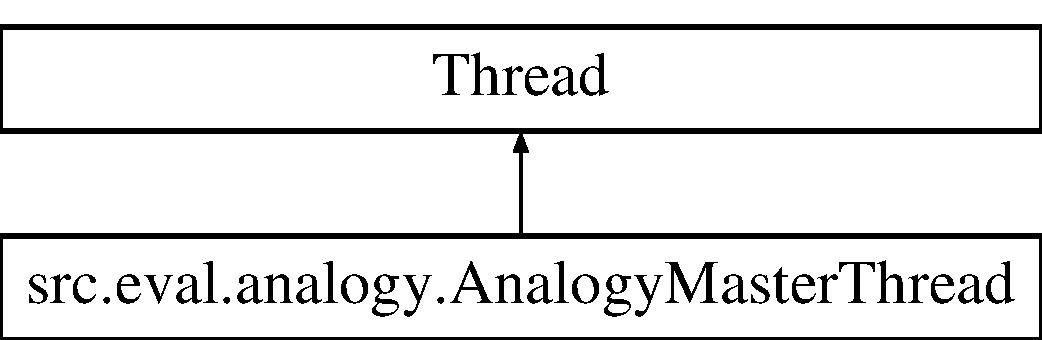
\includegraphics[height=2.000000cm]{classsrc_1_1eval_1_1analogy_1_1_analogy_master_thread}
\end{center}
\end{figure}
\subsection*{Public Member Functions}
\begin{DoxyCompactItemize}
\item 
def \hyperlink{classsrc_1_1eval_1_1analogy_1_1_analogy_master_thread_a5dcad4f45137fd4c5c5bfaf0874eb61b}{\+\_\+\+\_\+init\+\_\+\+\_\+} (self, \hyperlink{classsrc_1_1eval_1_1analogy_1_1_analogy_master_thread_a581000df6b13c7b2d3a06a56097972f0}{vector\+\_\+inpath}, \hyperlink{classsrc_1_1eval_1_1analogy_1_1_analogy_master_thread_aa76e56284b44372302314cbd82acedd0}{analogy\+\_\+path}, \hyperlink{classsrc_1_1eval_1_1analogy_1_1_analogy_master_thread_a32028e35b91d6f3b1338aed361a9b608}{per\+\_\+section}, \hyperlink{classsrc_1_1eval_1_1analogy_1_1_analogy_master_thread_a7ef0cbb224a26fc5ccd20887e0d039d4}{logpath}, \hyperlink{classsrc_1_1eval_1_1analogy_1_1_analogy_master_thread_a5a42ba2f5b1620a230e19597d3e2492b}{n})
\item 
def \hyperlink{classsrc_1_1eval_1_1analogy_1_1_analogy_master_thread_a594eee873738ea9191b686318cc8495f}{start\+\_\+threads} (self)
\item 
def \hyperlink{classsrc_1_1eval_1_1analogy_1_1_analogy_master_thread_a0d807197214f4dfc7ad77089acd220da}{prepare} (self)
\end{DoxyCompactItemize}
\subsection*{Public Attributes}
\begin{DoxyCompactItemize}
\item 
\hyperlink{classsrc_1_1eval_1_1analogy_1_1_analogy_master_thread_a581000df6b13c7b2d3a06a56097972f0}{vector\+\_\+inpath}
\item 
\hyperlink{classsrc_1_1eval_1_1analogy_1_1_analogy_master_thread_aa76e56284b44372302314cbd82acedd0}{analogy\+\_\+path}
\item 
\hyperlink{classsrc_1_1eval_1_1analogy_1_1_analogy_master_thread_a32028e35b91d6f3b1338aed361a9b608}{per\+\_\+section}
\item 
\hyperlink{classsrc_1_1eval_1_1analogy_1_1_analogy_master_thread_a7ef0cbb224a26fc5ccd20887e0d039d4}{logpath}
\item 
\hyperlink{classsrc_1_1eval_1_1analogy_1_1_analogy_master_thread_a5a42ba2f5b1620a230e19597d3e2492b}{n}
\item 
\hyperlink{classsrc_1_1eval_1_1analogy_1_1_analogy_master_thread_a093ad956946c45477e62df9e95460128}{threads}
\item 
\hyperlink{classsrc_1_1eval_1_1analogy_1_1_analogy_master_thread_a9d2e9c082fe78faf02948e0a0b357c21}{queues}
\item 
\hyperlink{classsrc_1_1eval_1_1analogy_1_1_analogy_master_thread_ac6084419ab7972b1ffc22a3756db3803}{model}
\end{DoxyCompactItemize}


\subsection{Constructor \& Destructor Documentation}
\index{src\+::eval\+::analogy\+::\+Analogy\+Master\+Thread@{src\+::eval\+::analogy\+::\+Analogy\+Master\+Thread}!\+\_\+\+\_\+init\+\_\+\+\_\+@{\+\_\+\+\_\+init\+\_\+\+\_\+}}
\index{\+\_\+\+\_\+init\+\_\+\+\_\+@{\+\_\+\+\_\+init\+\_\+\+\_\+}!src\+::eval\+::analogy\+::\+Analogy\+Master\+Thread@{src\+::eval\+::analogy\+::\+Analogy\+Master\+Thread}}
\subsubsection[{\texorpdfstring{\+\_\+\+\_\+init\+\_\+\+\_\+(self, vector\+\_\+inpath, analogy\+\_\+path, per\+\_\+section, logpath, n)}{\_\_init\_\_(self, vector\_inpath, analogy\_path, per\_section, logpath, n)}}]{\setlength{\rightskip}{0pt plus 5cm}def src.\+eval.\+analogy.\+Analogy\+Master\+Thread.\+\_\+\+\_\+init\+\_\+\+\_\+ (
\begin{DoxyParamCaption}
\item[{}]{self, }
\item[{}]{vector\+\_\+inpath, }
\item[{}]{analogy\+\_\+path, }
\item[{}]{per\+\_\+section, }
\item[{}]{logpath, }
\item[{}]{n}
\end{DoxyParamCaption}
)}\hypertarget{classsrc_1_1eval_1_1analogy_1_1_analogy_master_thread_a5dcad4f45137fd4c5c5bfaf0874eb61b}{}\label{classsrc_1_1eval_1_1analogy_1_1_analogy_master_thread_a5dcad4f45137fd4c5c5bfaf0874eb61b}


\subsection{Member Function Documentation}
\index{src\+::eval\+::analogy\+::\+Analogy\+Master\+Thread@{src\+::eval\+::analogy\+::\+Analogy\+Master\+Thread}!prepare@{prepare}}
\index{prepare@{prepare}!src\+::eval\+::analogy\+::\+Analogy\+Master\+Thread@{src\+::eval\+::analogy\+::\+Analogy\+Master\+Thread}}
\subsubsection[{\texorpdfstring{prepare(self)}{prepare(self)}}]{\setlength{\rightskip}{0pt plus 5cm}def src.\+eval.\+analogy.\+Analogy\+Master\+Thread.\+prepare (
\begin{DoxyParamCaption}
\item[{}]{self}
\end{DoxyParamCaption}
)}\hypertarget{classsrc_1_1eval_1_1analogy_1_1_analogy_master_thread_a0d807197214f4dfc7ad77089acd220da}{}\label{classsrc_1_1eval_1_1analogy_1_1_analogy_master_thread_a0d807197214f4dfc7ad77089acd220da}
\index{src\+::eval\+::analogy\+::\+Analogy\+Master\+Thread@{src\+::eval\+::analogy\+::\+Analogy\+Master\+Thread}!start\+\_\+threads@{start\+\_\+threads}}
\index{start\+\_\+threads@{start\+\_\+threads}!src\+::eval\+::analogy\+::\+Analogy\+Master\+Thread@{src\+::eval\+::analogy\+::\+Analogy\+Master\+Thread}}
\subsubsection[{\texorpdfstring{start\+\_\+threads(self)}{start\_threads(self)}}]{\setlength{\rightskip}{0pt plus 5cm}def src.\+eval.\+analogy.\+Analogy\+Master\+Thread.\+start\+\_\+threads (
\begin{DoxyParamCaption}
\item[{}]{self}
\end{DoxyParamCaption}
)}\hypertarget{classsrc_1_1eval_1_1analogy_1_1_analogy_master_thread_a594eee873738ea9191b686318cc8495f}{}\label{classsrc_1_1eval_1_1analogy_1_1_analogy_master_thread_a594eee873738ea9191b686318cc8495f}


\subsection{Member Data Documentation}
\index{src\+::eval\+::analogy\+::\+Analogy\+Master\+Thread@{src\+::eval\+::analogy\+::\+Analogy\+Master\+Thread}!analogy\+\_\+path@{analogy\+\_\+path}}
\index{analogy\+\_\+path@{analogy\+\_\+path}!src\+::eval\+::analogy\+::\+Analogy\+Master\+Thread@{src\+::eval\+::analogy\+::\+Analogy\+Master\+Thread}}
\subsubsection[{\texorpdfstring{analogy\+\_\+path}{analogy\_path}}]{\setlength{\rightskip}{0pt plus 5cm}src.\+eval.\+analogy.\+Analogy\+Master\+Thread.\+analogy\+\_\+path}\hypertarget{classsrc_1_1eval_1_1analogy_1_1_analogy_master_thread_aa76e56284b44372302314cbd82acedd0}{}\label{classsrc_1_1eval_1_1analogy_1_1_analogy_master_thread_aa76e56284b44372302314cbd82acedd0}
\index{src\+::eval\+::analogy\+::\+Analogy\+Master\+Thread@{src\+::eval\+::analogy\+::\+Analogy\+Master\+Thread}!logpath@{logpath}}
\index{logpath@{logpath}!src\+::eval\+::analogy\+::\+Analogy\+Master\+Thread@{src\+::eval\+::analogy\+::\+Analogy\+Master\+Thread}}
\subsubsection[{\texorpdfstring{logpath}{logpath}}]{\setlength{\rightskip}{0pt plus 5cm}src.\+eval.\+analogy.\+Analogy\+Master\+Thread.\+logpath}\hypertarget{classsrc_1_1eval_1_1analogy_1_1_analogy_master_thread_a7ef0cbb224a26fc5ccd20887e0d039d4}{}\label{classsrc_1_1eval_1_1analogy_1_1_analogy_master_thread_a7ef0cbb224a26fc5ccd20887e0d039d4}
\index{src\+::eval\+::analogy\+::\+Analogy\+Master\+Thread@{src\+::eval\+::analogy\+::\+Analogy\+Master\+Thread}!model@{model}}
\index{model@{model}!src\+::eval\+::analogy\+::\+Analogy\+Master\+Thread@{src\+::eval\+::analogy\+::\+Analogy\+Master\+Thread}}
\subsubsection[{\texorpdfstring{model}{model}}]{\setlength{\rightskip}{0pt plus 5cm}src.\+eval.\+analogy.\+Analogy\+Master\+Thread.\+model}\hypertarget{classsrc_1_1eval_1_1analogy_1_1_analogy_master_thread_ac6084419ab7972b1ffc22a3756db3803}{}\label{classsrc_1_1eval_1_1analogy_1_1_analogy_master_thread_ac6084419ab7972b1ffc22a3756db3803}
\index{src\+::eval\+::analogy\+::\+Analogy\+Master\+Thread@{src\+::eval\+::analogy\+::\+Analogy\+Master\+Thread}!n@{n}}
\index{n@{n}!src\+::eval\+::analogy\+::\+Analogy\+Master\+Thread@{src\+::eval\+::analogy\+::\+Analogy\+Master\+Thread}}
\subsubsection[{\texorpdfstring{n}{n}}]{\setlength{\rightskip}{0pt plus 5cm}src.\+eval.\+analogy.\+Analogy\+Master\+Thread.\+n}\hypertarget{classsrc_1_1eval_1_1analogy_1_1_analogy_master_thread_a5a42ba2f5b1620a230e19597d3e2492b}{}\label{classsrc_1_1eval_1_1analogy_1_1_analogy_master_thread_a5a42ba2f5b1620a230e19597d3e2492b}
\index{src\+::eval\+::analogy\+::\+Analogy\+Master\+Thread@{src\+::eval\+::analogy\+::\+Analogy\+Master\+Thread}!per\+\_\+section@{per\+\_\+section}}
\index{per\+\_\+section@{per\+\_\+section}!src\+::eval\+::analogy\+::\+Analogy\+Master\+Thread@{src\+::eval\+::analogy\+::\+Analogy\+Master\+Thread}}
\subsubsection[{\texorpdfstring{per\+\_\+section}{per\_section}}]{\setlength{\rightskip}{0pt plus 5cm}src.\+eval.\+analogy.\+Analogy\+Master\+Thread.\+per\+\_\+section}\hypertarget{classsrc_1_1eval_1_1analogy_1_1_analogy_master_thread_a32028e35b91d6f3b1338aed361a9b608}{}\label{classsrc_1_1eval_1_1analogy_1_1_analogy_master_thread_a32028e35b91d6f3b1338aed361a9b608}
\index{src\+::eval\+::analogy\+::\+Analogy\+Master\+Thread@{src\+::eval\+::analogy\+::\+Analogy\+Master\+Thread}!queues@{queues}}
\index{queues@{queues}!src\+::eval\+::analogy\+::\+Analogy\+Master\+Thread@{src\+::eval\+::analogy\+::\+Analogy\+Master\+Thread}}
\subsubsection[{\texorpdfstring{queues}{queues}}]{\setlength{\rightskip}{0pt plus 5cm}src.\+eval.\+analogy.\+Analogy\+Master\+Thread.\+queues}\hypertarget{classsrc_1_1eval_1_1analogy_1_1_analogy_master_thread_a9d2e9c082fe78faf02948e0a0b357c21}{}\label{classsrc_1_1eval_1_1analogy_1_1_analogy_master_thread_a9d2e9c082fe78faf02948e0a0b357c21}
\index{src\+::eval\+::analogy\+::\+Analogy\+Master\+Thread@{src\+::eval\+::analogy\+::\+Analogy\+Master\+Thread}!threads@{threads}}
\index{threads@{threads}!src\+::eval\+::analogy\+::\+Analogy\+Master\+Thread@{src\+::eval\+::analogy\+::\+Analogy\+Master\+Thread}}
\subsubsection[{\texorpdfstring{threads}{threads}}]{\setlength{\rightskip}{0pt plus 5cm}src.\+eval.\+analogy.\+Analogy\+Master\+Thread.\+threads}\hypertarget{classsrc_1_1eval_1_1analogy_1_1_analogy_master_thread_a093ad956946c45477e62df9e95460128}{}\label{classsrc_1_1eval_1_1analogy_1_1_analogy_master_thread_a093ad956946c45477e62df9e95460128}
\index{src\+::eval\+::analogy\+::\+Analogy\+Master\+Thread@{src\+::eval\+::analogy\+::\+Analogy\+Master\+Thread}!vector\+\_\+inpath@{vector\+\_\+inpath}}
\index{vector\+\_\+inpath@{vector\+\_\+inpath}!src\+::eval\+::analogy\+::\+Analogy\+Master\+Thread@{src\+::eval\+::analogy\+::\+Analogy\+Master\+Thread}}
\subsubsection[{\texorpdfstring{vector\+\_\+inpath}{vector\_inpath}}]{\setlength{\rightskip}{0pt plus 5cm}src.\+eval.\+analogy.\+Analogy\+Master\+Thread.\+vector\+\_\+inpath}\hypertarget{classsrc_1_1eval_1_1analogy_1_1_analogy_master_thread_a581000df6b13c7b2d3a06a56097972f0}{}\label{classsrc_1_1eval_1_1analogy_1_1_analogy_master_thread_a581000df6b13c7b2d3a06a56097972f0}


The documentation for this class was generated from the following file\+:\begin{DoxyCompactItemize}
\item 
/\+Users/dennisulmer/\+Documents/\+Studium/7. Semester/\+Computerlinguistik/\+Bachelorarbeit/src/eval/\hyperlink{analogy_8py}{analogy.\+py}\end{DoxyCompactItemize}

\hypertarget{classsrc_1_1eval_1_1analogy_1_1_analogy_worker_thread}{}\section{src.\+eval.\+analogy.\+Analogy\+Worker\+Thread Class Reference}
\label{classsrc_1_1eval_1_1analogy_1_1_analogy_worker_thread}\index{src.\+eval.\+analogy.\+Analogy\+Worker\+Thread@{src.\+eval.\+analogy.\+Analogy\+Worker\+Thread}}
Inheritance diagram for src.\+eval.\+analogy.\+Analogy\+Worker\+Thread\+:\begin{figure}[H]
\begin{center}
\leavevmode
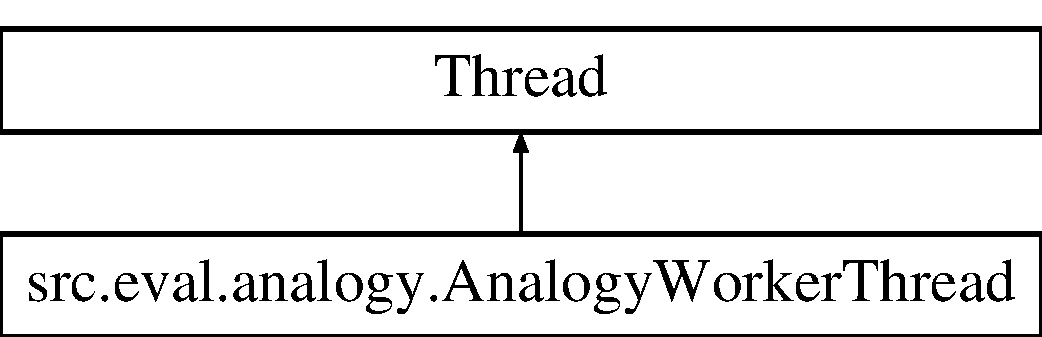
\includegraphics[height=2.000000cm]{classsrc_1_1eval_1_1analogy_1_1_analogy_worker_thread}
\end{center}
\end{figure}
\subsection*{Public Member Functions}
\begin{DoxyCompactItemize}
\item 
def \hyperlink{classsrc_1_1eval_1_1analogy_1_1_analogy_worker_thread_a8c02b7e5589b607622f4f2e69db5eec0}{\+\_\+\+\_\+init\+\_\+\+\_\+} (self, \hyperlink{classsrc_1_1eval_1_1analogy_1_1_analogy_worker_thread_a8b2c2720d9c294ddc0b020ad64174e6f}{worker\+\_\+id}, \hyperlink{classsrc_1_1eval_1_1analogy_1_1_analogy_worker_thread_aab57ebb5a41ee124300ac2125083bf3d}{model})
\item 
def \hyperlink{classsrc_1_1eval_1_1analogy_1_1_analogy_worker_thread_a4f959a591d5130eeb6a03ef2545c8756}{run} (self)
\item 
def \hyperlink{classsrc_1_1eval_1_1analogy_1_1_analogy_worker_thread_af2f9a01892a4dd4fa2ff8e87114b7b08}{find\+\_\+most\+\_\+similar\+\_\+cosmul} (self, a, a\+\_\+, b)
\end{DoxyCompactItemize}
\subsection*{Public Attributes}
\begin{DoxyCompactItemize}
\item 
\hyperlink{classsrc_1_1eval_1_1analogy_1_1_analogy_worker_thread_a8b2c2720d9c294ddc0b020ad64174e6f}{worker\+\_\+id}
\item 
\hyperlink{classsrc_1_1eval_1_1analogy_1_1_analogy_worker_thread_aab57ebb5a41ee124300ac2125083bf3d}{model}
\item 
\hyperlink{classsrc_1_1eval_1_1analogy_1_1_analogy_worker_thread_a9e2176d75b98d24be7b5d4c4c6022e29}{finished}
\item 
\hyperlink{classsrc_1_1eval_1_1analogy_1_1_analogy_worker_thread_a28cd46825684dfb20e0a56da7d5c469a}{current\+\_\+queue}
\item 
\hyperlink{classsrc_1_1eval_1_1analogy_1_1_analogy_worker_thread_a8d27081ea882e7a4ad24d760a16529d8}{n}
\item 
\hyperlink{classsrc_1_1eval_1_1analogy_1_1_analogy_worker_thread_a966ad902db2b4f57b40c77fc8582312b}{fail}
\item 
\hyperlink{classsrc_1_1eval_1_1analogy_1_1_analogy_worker_thread_af2ff7bed2042439b7d31aabaec568fc5}{errors}
\end{DoxyCompactItemize}


\subsection{Constructor \& Destructor Documentation}
\index{src\+::eval\+::analogy\+::\+Analogy\+Worker\+Thread@{src\+::eval\+::analogy\+::\+Analogy\+Worker\+Thread}!\+\_\+\+\_\+init\+\_\+\+\_\+@{\+\_\+\+\_\+init\+\_\+\+\_\+}}
\index{\+\_\+\+\_\+init\+\_\+\+\_\+@{\+\_\+\+\_\+init\+\_\+\+\_\+}!src\+::eval\+::analogy\+::\+Analogy\+Worker\+Thread@{src\+::eval\+::analogy\+::\+Analogy\+Worker\+Thread}}
\subsubsection[{\texorpdfstring{\+\_\+\+\_\+init\+\_\+\+\_\+(self, worker\+\_\+id, model)}{\_\_init\_\_(self, worker\_id, model)}}]{\setlength{\rightskip}{0pt plus 5cm}def src.\+eval.\+analogy.\+Analogy\+Worker\+Thread.\+\_\+\+\_\+init\+\_\+\+\_\+ (
\begin{DoxyParamCaption}
\item[{}]{self, }
\item[{}]{worker\+\_\+id, }
\item[{}]{model}
\end{DoxyParamCaption}
)}\hypertarget{classsrc_1_1eval_1_1analogy_1_1_analogy_worker_thread_a8c02b7e5589b607622f4f2e69db5eec0}{}\label{classsrc_1_1eval_1_1analogy_1_1_analogy_worker_thread_a8c02b7e5589b607622f4f2e69db5eec0}


\subsection{Member Function Documentation}
\index{src\+::eval\+::analogy\+::\+Analogy\+Worker\+Thread@{src\+::eval\+::analogy\+::\+Analogy\+Worker\+Thread}!find\+\_\+most\+\_\+similar\+\_\+cosmul@{find\+\_\+most\+\_\+similar\+\_\+cosmul}}
\index{find\+\_\+most\+\_\+similar\+\_\+cosmul@{find\+\_\+most\+\_\+similar\+\_\+cosmul}!src\+::eval\+::analogy\+::\+Analogy\+Worker\+Thread@{src\+::eval\+::analogy\+::\+Analogy\+Worker\+Thread}}
\subsubsection[{\texorpdfstring{find\+\_\+most\+\_\+similar\+\_\+cosmul(self, a, a\+\_\+, b)}{find\_most\_similar\_cosmul(self, a, a\_, b)}}]{\setlength{\rightskip}{0pt plus 5cm}def src.\+eval.\+analogy.\+Analogy\+Worker\+Thread.\+find\+\_\+most\+\_\+similar\+\_\+cosmul (
\begin{DoxyParamCaption}
\item[{}]{self, }
\item[{}]{a, }
\item[{}]{a\+\_\+, }
\item[{}]{b}
\end{DoxyParamCaption}
)}\hypertarget{classsrc_1_1eval_1_1analogy_1_1_analogy_worker_thread_af2f9a01892a4dd4fa2ff8e87114b7b08}{}\label{classsrc_1_1eval_1_1analogy_1_1_analogy_worker_thread_af2f9a01892a4dd4fa2ff8e87114b7b08}
\index{src\+::eval\+::analogy\+::\+Analogy\+Worker\+Thread@{src\+::eval\+::analogy\+::\+Analogy\+Worker\+Thread}!run@{run}}
\index{run@{run}!src\+::eval\+::analogy\+::\+Analogy\+Worker\+Thread@{src\+::eval\+::analogy\+::\+Analogy\+Worker\+Thread}}
\subsubsection[{\texorpdfstring{run(self)}{run(self)}}]{\setlength{\rightskip}{0pt plus 5cm}def src.\+eval.\+analogy.\+Analogy\+Worker\+Thread.\+run (
\begin{DoxyParamCaption}
\item[{}]{self}
\end{DoxyParamCaption}
)}\hypertarget{classsrc_1_1eval_1_1analogy_1_1_analogy_worker_thread_a4f959a591d5130eeb6a03ef2545c8756}{}\label{classsrc_1_1eval_1_1analogy_1_1_analogy_worker_thread_a4f959a591d5130eeb6a03ef2545c8756}


\subsection{Member Data Documentation}
\index{src\+::eval\+::analogy\+::\+Analogy\+Worker\+Thread@{src\+::eval\+::analogy\+::\+Analogy\+Worker\+Thread}!current\+\_\+queue@{current\+\_\+queue}}
\index{current\+\_\+queue@{current\+\_\+queue}!src\+::eval\+::analogy\+::\+Analogy\+Worker\+Thread@{src\+::eval\+::analogy\+::\+Analogy\+Worker\+Thread}}
\subsubsection[{\texorpdfstring{current\+\_\+queue}{current\_queue}}]{\setlength{\rightskip}{0pt plus 5cm}src.\+eval.\+analogy.\+Analogy\+Worker\+Thread.\+current\+\_\+queue}\hypertarget{classsrc_1_1eval_1_1analogy_1_1_analogy_worker_thread_a28cd46825684dfb20e0a56da7d5c469a}{}\label{classsrc_1_1eval_1_1analogy_1_1_analogy_worker_thread_a28cd46825684dfb20e0a56da7d5c469a}
\index{src\+::eval\+::analogy\+::\+Analogy\+Worker\+Thread@{src\+::eval\+::analogy\+::\+Analogy\+Worker\+Thread}!errors@{errors}}
\index{errors@{errors}!src\+::eval\+::analogy\+::\+Analogy\+Worker\+Thread@{src\+::eval\+::analogy\+::\+Analogy\+Worker\+Thread}}
\subsubsection[{\texorpdfstring{errors}{errors}}]{\setlength{\rightskip}{0pt plus 5cm}src.\+eval.\+analogy.\+Analogy\+Worker\+Thread.\+errors}\hypertarget{classsrc_1_1eval_1_1analogy_1_1_analogy_worker_thread_af2ff7bed2042439b7d31aabaec568fc5}{}\label{classsrc_1_1eval_1_1analogy_1_1_analogy_worker_thread_af2ff7bed2042439b7d31aabaec568fc5}
\index{src\+::eval\+::analogy\+::\+Analogy\+Worker\+Thread@{src\+::eval\+::analogy\+::\+Analogy\+Worker\+Thread}!fail@{fail}}
\index{fail@{fail}!src\+::eval\+::analogy\+::\+Analogy\+Worker\+Thread@{src\+::eval\+::analogy\+::\+Analogy\+Worker\+Thread}}
\subsubsection[{\texorpdfstring{fail}{fail}}]{\setlength{\rightskip}{0pt plus 5cm}src.\+eval.\+analogy.\+Analogy\+Worker\+Thread.\+fail}\hypertarget{classsrc_1_1eval_1_1analogy_1_1_analogy_worker_thread_a966ad902db2b4f57b40c77fc8582312b}{}\label{classsrc_1_1eval_1_1analogy_1_1_analogy_worker_thread_a966ad902db2b4f57b40c77fc8582312b}
\index{src\+::eval\+::analogy\+::\+Analogy\+Worker\+Thread@{src\+::eval\+::analogy\+::\+Analogy\+Worker\+Thread}!finished@{finished}}
\index{finished@{finished}!src\+::eval\+::analogy\+::\+Analogy\+Worker\+Thread@{src\+::eval\+::analogy\+::\+Analogy\+Worker\+Thread}}
\subsubsection[{\texorpdfstring{finished}{finished}}]{\setlength{\rightskip}{0pt plus 5cm}src.\+eval.\+analogy.\+Analogy\+Worker\+Thread.\+finished}\hypertarget{classsrc_1_1eval_1_1analogy_1_1_analogy_worker_thread_a9e2176d75b98d24be7b5d4c4c6022e29}{}\label{classsrc_1_1eval_1_1analogy_1_1_analogy_worker_thread_a9e2176d75b98d24be7b5d4c4c6022e29}
\index{src\+::eval\+::analogy\+::\+Analogy\+Worker\+Thread@{src\+::eval\+::analogy\+::\+Analogy\+Worker\+Thread}!model@{model}}
\index{model@{model}!src\+::eval\+::analogy\+::\+Analogy\+Worker\+Thread@{src\+::eval\+::analogy\+::\+Analogy\+Worker\+Thread}}
\subsubsection[{\texorpdfstring{model}{model}}]{\setlength{\rightskip}{0pt plus 5cm}src.\+eval.\+analogy.\+Analogy\+Worker\+Thread.\+model}\hypertarget{classsrc_1_1eval_1_1analogy_1_1_analogy_worker_thread_aab57ebb5a41ee124300ac2125083bf3d}{}\label{classsrc_1_1eval_1_1analogy_1_1_analogy_worker_thread_aab57ebb5a41ee124300ac2125083bf3d}
\index{src\+::eval\+::analogy\+::\+Analogy\+Worker\+Thread@{src\+::eval\+::analogy\+::\+Analogy\+Worker\+Thread}!n@{n}}
\index{n@{n}!src\+::eval\+::analogy\+::\+Analogy\+Worker\+Thread@{src\+::eval\+::analogy\+::\+Analogy\+Worker\+Thread}}
\subsubsection[{\texorpdfstring{n}{n}}]{\setlength{\rightskip}{0pt plus 5cm}src.\+eval.\+analogy.\+Analogy\+Worker\+Thread.\+n}\hypertarget{classsrc_1_1eval_1_1analogy_1_1_analogy_worker_thread_a8d27081ea882e7a4ad24d760a16529d8}{}\label{classsrc_1_1eval_1_1analogy_1_1_analogy_worker_thread_a8d27081ea882e7a4ad24d760a16529d8}
\index{src\+::eval\+::analogy\+::\+Analogy\+Worker\+Thread@{src\+::eval\+::analogy\+::\+Analogy\+Worker\+Thread}!worker\+\_\+id@{worker\+\_\+id}}
\index{worker\+\_\+id@{worker\+\_\+id}!src\+::eval\+::analogy\+::\+Analogy\+Worker\+Thread@{src\+::eval\+::analogy\+::\+Analogy\+Worker\+Thread}}
\subsubsection[{\texorpdfstring{worker\+\_\+id}{worker\_id}}]{\setlength{\rightskip}{0pt plus 5cm}src.\+eval.\+analogy.\+Analogy\+Worker\+Thread.\+worker\+\_\+id}\hypertarget{classsrc_1_1eval_1_1analogy_1_1_analogy_worker_thread_a8b2c2720d9c294ddc0b020ad64174e6f}{}\label{classsrc_1_1eval_1_1analogy_1_1_analogy_worker_thread_a8b2c2720d9c294ddc0b020ad64174e6f}


The documentation for this class was generated from the following file\+:\begin{DoxyCompactItemize}
\item 
/\+Users/dennisulmer/\+Documents/\+Studium/7. Semester/\+Computerlinguistik/\+Bachelorarbeit/src/eval/\hyperlink{analogy_8py}{analogy.\+py}\end{DoxyCompactItemize}

\hypertarget{classsrc_1_1mapping_1_1mapthreading_1_1_mapping_master_thread}{}\section{src.\+mapping.\+mapthreading.\+Mapping\+Master\+Thread Class Reference}
\label{classsrc_1_1mapping_1_1mapthreading_1_1_mapping_master_thread}\index{src.\+mapping.\+mapthreading.\+Mapping\+Master\+Thread@{src.\+mapping.\+mapthreading.\+Mapping\+Master\+Thread}}
Inheritance diagram for src.\+mapping.\+mapthreading.\+Mapping\+Master\+Thread\+:\begin{figure}[H]
\begin{center}
\leavevmode
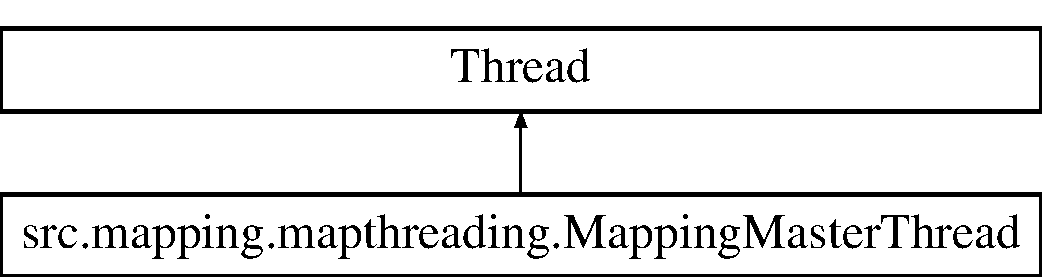
\includegraphics[height=2.000000cm]{classsrc_1_1mapping_1_1mapthreading_1_1_mapping_master_thread}
\end{center}
\end{figure}
\subsection*{Public Member Functions}
\begin{DoxyCompactItemize}
\item 
def \hyperlink{classsrc_1_1mapping_1_1mapthreading_1_1_mapping_master_thread_a71b5c2e61bf13cffdcc0801a7f5a7121}{\+\_\+\+\_\+init\+\_\+\+\_\+} (self, n, \hyperlink{classsrc_1_1mapping_1_1mapthreading_1_1_mapping_master_thread_ad28cd816fab3ea85e9b7f9c105d306a2}{vector\+\_\+inpath}, \hyperlink{classsrc_1_1mapping_1_1mapthreading_1_1_mapping_master_thread_a38c9150229ea50de973f9f4ce2e6569f}{vector\+\_\+outpath}, \hyperlink{classsrc_1_1mapping_1_1mapthreading_1_1_mapping_master_thread_a57fe84be32a92ff596ca24b0a7de2324}{features}, \hyperlink{classsrc_1_1mapping_1_1mapthreading_1_1_mapping_master_thread_ac2d586e34cbeeeb50f653ad0cd0596fa}{ids\+\_\+inpath}, \hyperlink{classsrc_1_1mapping_1_1mapthreading_1_1_mapping_master_thread_a88fb8c0056df70baf0f4c3fa20d8807e}{indices\+\_\+inpath})
\item 
def \hyperlink{classsrc_1_1mapping_1_1mapthreading_1_1_mapping_master_thread_adba41bbaf55d33182698846fffb1883c}{start\+\_\+threads} (self)
\item 
def \hyperlink{classsrc_1_1mapping_1_1mapthreading_1_1_mapping_master_thread_ab0dd772e890149f3a961e81d4b9bdb83}{prepare} (self)
\item 
def \hyperlink{classsrc_1_1mapping_1_1mapthreading_1_1_mapping_master_thread_ab95b1d8a372ec75738a5ac67a7c752d6}{read\+\_\+ids\+\_\+file} (self, \hyperlink{classsrc_1_1mapping_1_1mapthreading_1_1_mapping_master_thread_ac2d586e34cbeeeb50f653ad0cd0596fa}{ids\+\_\+inpath})
\end{DoxyCompactItemize}
\subsection*{Public Attributes}
\begin{DoxyCompactItemize}
\item 
\hyperlink{classsrc_1_1mapping_1_1mapthreading_1_1_mapping_master_thread_ad28cd816fab3ea85e9b7f9c105d306a2}{vector\+\_\+inpath}
\item 
\hyperlink{classsrc_1_1mapping_1_1mapthreading_1_1_mapping_master_thread_a38c9150229ea50de973f9f4ce2e6569f}{vector\+\_\+outpath}
\item 
\hyperlink{classsrc_1_1mapping_1_1mapthreading_1_1_mapping_master_thread_ac2d586e34cbeeeb50f653ad0cd0596fa}{ids\+\_\+inpath}
\item 
\hyperlink{classsrc_1_1mapping_1_1mapthreading_1_1_mapping_master_thread_a88fb8c0056df70baf0f4c3fa20d8807e}{indices\+\_\+inpath}
\item 
\hyperlink{classsrc_1_1mapping_1_1mapthreading_1_1_mapping_master_thread_ad7241d90991759aa3f991ac6b3c7262d}{vector\+\_\+queue}
\item 
\hyperlink{classsrc_1_1mapping_1_1mapthreading_1_1_mapping_master_thread_a96d361c570dffb2a12aa2438ea282ff4}{vector\+\_\+dict}
\item 
\hyperlink{classsrc_1_1mapping_1_1mapthreading_1_1_mapping_master_thread_a9590c2f02cc5fbb8b04cea323b9ae51b}{occurrences}
\item 
\hyperlink{classsrc_1_1mapping_1_1mapthreading_1_1_mapping_master_thread_aa2df8eb426374f62553139fee7b107f6}{indices}
\item 
\hyperlink{classsrc_1_1mapping_1_1mapthreading_1_1_mapping_master_thread_a57fe84be32a92ff596ca24b0a7de2324}{features}
\item 
\hyperlink{classsrc_1_1mapping_1_1mapthreading_1_1_mapping_master_thread_afffeaf170582fa3bb01f14ac4037a1f8}{coc}
\item 
\hyperlink{classsrc_1_1mapping_1_1mapthreading_1_1_mapping_master_thread_aec87bfdd4a2d97c8ac2370ca064b57b9}{ind}
\item 
\hyperlink{classsrc_1_1mapping_1_1mapthreading_1_1_mapping_master_thread_a0dc846ca67326784955baccaf10b96bd}{threads}
\end{DoxyCompactItemize}


\subsection{Constructor \& Destructor Documentation}
\index{src\+::mapping\+::mapthreading\+::\+Mapping\+Master\+Thread@{src\+::mapping\+::mapthreading\+::\+Mapping\+Master\+Thread}!\+\_\+\+\_\+init\+\_\+\+\_\+@{\+\_\+\+\_\+init\+\_\+\+\_\+}}
\index{\+\_\+\+\_\+init\+\_\+\+\_\+@{\+\_\+\+\_\+init\+\_\+\+\_\+}!src\+::mapping\+::mapthreading\+::\+Mapping\+Master\+Thread@{src\+::mapping\+::mapthreading\+::\+Mapping\+Master\+Thread}}
\subsubsection[{\texorpdfstring{\+\_\+\+\_\+init\+\_\+\+\_\+(self, n, vector\+\_\+inpath, vector\+\_\+outpath, features, ids\+\_\+inpath, indices\+\_\+inpath)}{\_\_init\_\_(self, n, vector\_inpath, vector\_outpath, features, ids\_inpath, indices\_inpath)}}]{\setlength{\rightskip}{0pt plus 5cm}def src.\+mapping.\+mapthreading.\+Mapping\+Master\+Thread.\+\_\+\+\_\+init\+\_\+\+\_\+ (
\begin{DoxyParamCaption}
\item[{}]{self, }
\item[{}]{n, }
\item[{}]{vector\+\_\+inpath, }
\item[{}]{vector\+\_\+outpath, }
\item[{}]{features, }
\item[{}]{ids\+\_\+inpath, }
\item[{}]{indices\+\_\+inpath}
\end{DoxyParamCaption}
)}\hypertarget{classsrc_1_1mapping_1_1mapthreading_1_1_mapping_master_thread_a71b5c2e61bf13cffdcc0801a7f5a7121}{}\label{classsrc_1_1mapping_1_1mapthreading_1_1_mapping_master_thread_a71b5c2e61bf13cffdcc0801a7f5a7121}


\subsection{Member Function Documentation}
\index{src\+::mapping\+::mapthreading\+::\+Mapping\+Master\+Thread@{src\+::mapping\+::mapthreading\+::\+Mapping\+Master\+Thread}!prepare@{prepare}}
\index{prepare@{prepare}!src\+::mapping\+::mapthreading\+::\+Mapping\+Master\+Thread@{src\+::mapping\+::mapthreading\+::\+Mapping\+Master\+Thread}}
\subsubsection[{\texorpdfstring{prepare(self)}{prepare(self)}}]{\setlength{\rightskip}{0pt plus 5cm}def src.\+mapping.\+mapthreading.\+Mapping\+Master\+Thread.\+prepare (
\begin{DoxyParamCaption}
\item[{}]{self}
\end{DoxyParamCaption}
)}\hypertarget{classsrc_1_1mapping_1_1mapthreading_1_1_mapping_master_thread_ab0dd772e890149f3a961e81d4b9bdb83}{}\label{classsrc_1_1mapping_1_1mapthreading_1_1_mapping_master_thread_ab0dd772e890149f3a961e81d4b9bdb83}
\index{src\+::mapping\+::mapthreading\+::\+Mapping\+Master\+Thread@{src\+::mapping\+::mapthreading\+::\+Mapping\+Master\+Thread}!read\+\_\+ids\+\_\+file@{read\+\_\+ids\+\_\+file}}
\index{read\+\_\+ids\+\_\+file@{read\+\_\+ids\+\_\+file}!src\+::mapping\+::mapthreading\+::\+Mapping\+Master\+Thread@{src\+::mapping\+::mapthreading\+::\+Mapping\+Master\+Thread}}
\subsubsection[{\texorpdfstring{read\+\_\+ids\+\_\+file(self, ids\+\_\+inpath)}{read\_ids\_file(self, ids\_inpath)}}]{\setlength{\rightskip}{0pt plus 5cm}def src.\+mapping.\+mapthreading.\+Mapping\+Master\+Thread.\+read\+\_\+ids\+\_\+file (
\begin{DoxyParamCaption}
\item[{}]{self, }
\item[{}]{ids\+\_\+inpath}
\end{DoxyParamCaption}
)}\hypertarget{classsrc_1_1mapping_1_1mapthreading_1_1_mapping_master_thread_ab95b1d8a372ec75738a5ac67a7c752d6}{}\label{classsrc_1_1mapping_1_1mapthreading_1_1_mapping_master_thread_ab95b1d8a372ec75738a5ac67a7c752d6}
\index{src\+::mapping\+::mapthreading\+::\+Mapping\+Master\+Thread@{src\+::mapping\+::mapthreading\+::\+Mapping\+Master\+Thread}!start\+\_\+threads@{start\+\_\+threads}}
\index{start\+\_\+threads@{start\+\_\+threads}!src\+::mapping\+::mapthreading\+::\+Mapping\+Master\+Thread@{src\+::mapping\+::mapthreading\+::\+Mapping\+Master\+Thread}}
\subsubsection[{\texorpdfstring{start\+\_\+threads(self)}{start\_threads(self)}}]{\setlength{\rightskip}{0pt plus 5cm}def src.\+mapping.\+mapthreading.\+Mapping\+Master\+Thread.\+start\+\_\+threads (
\begin{DoxyParamCaption}
\item[{}]{self}
\end{DoxyParamCaption}
)}\hypertarget{classsrc_1_1mapping_1_1mapthreading_1_1_mapping_master_thread_adba41bbaf55d33182698846fffb1883c}{}\label{classsrc_1_1mapping_1_1mapthreading_1_1_mapping_master_thread_adba41bbaf55d33182698846fffb1883c}


\subsection{Member Data Documentation}
\index{src\+::mapping\+::mapthreading\+::\+Mapping\+Master\+Thread@{src\+::mapping\+::mapthreading\+::\+Mapping\+Master\+Thread}!coc@{coc}}
\index{coc@{coc}!src\+::mapping\+::mapthreading\+::\+Mapping\+Master\+Thread@{src\+::mapping\+::mapthreading\+::\+Mapping\+Master\+Thread}}
\subsubsection[{\texorpdfstring{coc}{coc}}]{\setlength{\rightskip}{0pt plus 5cm}src.\+mapping.\+mapthreading.\+Mapping\+Master\+Thread.\+coc}\hypertarget{classsrc_1_1mapping_1_1mapthreading_1_1_mapping_master_thread_afffeaf170582fa3bb01f14ac4037a1f8}{}\label{classsrc_1_1mapping_1_1mapthreading_1_1_mapping_master_thread_afffeaf170582fa3bb01f14ac4037a1f8}
\index{src\+::mapping\+::mapthreading\+::\+Mapping\+Master\+Thread@{src\+::mapping\+::mapthreading\+::\+Mapping\+Master\+Thread}!features@{features}}
\index{features@{features}!src\+::mapping\+::mapthreading\+::\+Mapping\+Master\+Thread@{src\+::mapping\+::mapthreading\+::\+Mapping\+Master\+Thread}}
\subsubsection[{\texorpdfstring{features}{features}}]{\setlength{\rightskip}{0pt plus 5cm}src.\+mapping.\+mapthreading.\+Mapping\+Master\+Thread.\+features}\hypertarget{classsrc_1_1mapping_1_1mapthreading_1_1_mapping_master_thread_a57fe84be32a92ff596ca24b0a7de2324}{}\label{classsrc_1_1mapping_1_1mapthreading_1_1_mapping_master_thread_a57fe84be32a92ff596ca24b0a7de2324}
\index{src\+::mapping\+::mapthreading\+::\+Mapping\+Master\+Thread@{src\+::mapping\+::mapthreading\+::\+Mapping\+Master\+Thread}!ids\+\_\+inpath@{ids\+\_\+inpath}}
\index{ids\+\_\+inpath@{ids\+\_\+inpath}!src\+::mapping\+::mapthreading\+::\+Mapping\+Master\+Thread@{src\+::mapping\+::mapthreading\+::\+Mapping\+Master\+Thread}}
\subsubsection[{\texorpdfstring{ids\+\_\+inpath}{ids\_inpath}}]{\setlength{\rightskip}{0pt plus 5cm}src.\+mapping.\+mapthreading.\+Mapping\+Master\+Thread.\+ids\+\_\+inpath}\hypertarget{classsrc_1_1mapping_1_1mapthreading_1_1_mapping_master_thread_ac2d586e34cbeeeb50f653ad0cd0596fa}{}\label{classsrc_1_1mapping_1_1mapthreading_1_1_mapping_master_thread_ac2d586e34cbeeeb50f653ad0cd0596fa}
\index{src\+::mapping\+::mapthreading\+::\+Mapping\+Master\+Thread@{src\+::mapping\+::mapthreading\+::\+Mapping\+Master\+Thread}!ind@{ind}}
\index{ind@{ind}!src\+::mapping\+::mapthreading\+::\+Mapping\+Master\+Thread@{src\+::mapping\+::mapthreading\+::\+Mapping\+Master\+Thread}}
\subsubsection[{\texorpdfstring{ind}{ind}}]{\setlength{\rightskip}{0pt plus 5cm}src.\+mapping.\+mapthreading.\+Mapping\+Master\+Thread.\+ind}\hypertarget{classsrc_1_1mapping_1_1mapthreading_1_1_mapping_master_thread_aec87bfdd4a2d97c8ac2370ca064b57b9}{}\label{classsrc_1_1mapping_1_1mapthreading_1_1_mapping_master_thread_aec87bfdd4a2d97c8ac2370ca064b57b9}
\index{src\+::mapping\+::mapthreading\+::\+Mapping\+Master\+Thread@{src\+::mapping\+::mapthreading\+::\+Mapping\+Master\+Thread}!indices@{indices}}
\index{indices@{indices}!src\+::mapping\+::mapthreading\+::\+Mapping\+Master\+Thread@{src\+::mapping\+::mapthreading\+::\+Mapping\+Master\+Thread}}
\subsubsection[{\texorpdfstring{indices}{indices}}]{\setlength{\rightskip}{0pt plus 5cm}src.\+mapping.\+mapthreading.\+Mapping\+Master\+Thread.\+indices}\hypertarget{classsrc_1_1mapping_1_1mapthreading_1_1_mapping_master_thread_aa2df8eb426374f62553139fee7b107f6}{}\label{classsrc_1_1mapping_1_1mapthreading_1_1_mapping_master_thread_aa2df8eb426374f62553139fee7b107f6}
\index{src\+::mapping\+::mapthreading\+::\+Mapping\+Master\+Thread@{src\+::mapping\+::mapthreading\+::\+Mapping\+Master\+Thread}!indices\+\_\+inpath@{indices\+\_\+inpath}}
\index{indices\+\_\+inpath@{indices\+\_\+inpath}!src\+::mapping\+::mapthreading\+::\+Mapping\+Master\+Thread@{src\+::mapping\+::mapthreading\+::\+Mapping\+Master\+Thread}}
\subsubsection[{\texorpdfstring{indices\+\_\+inpath}{indices\_inpath}}]{\setlength{\rightskip}{0pt plus 5cm}src.\+mapping.\+mapthreading.\+Mapping\+Master\+Thread.\+indices\+\_\+inpath}\hypertarget{classsrc_1_1mapping_1_1mapthreading_1_1_mapping_master_thread_a88fb8c0056df70baf0f4c3fa20d8807e}{}\label{classsrc_1_1mapping_1_1mapthreading_1_1_mapping_master_thread_a88fb8c0056df70baf0f4c3fa20d8807e}
\index{src\+::mapping\+::mapthreading\+::\+Mapping\+Master\+Thread@{src\+::mapping\+::mapthreading\+::\+Mapping\+Master\+Thread}!occurrences@{occurrences}}
\index{occurrences@{occurrences}!src\+::mapping\+::mapthreading\+::\+Mapping\+Master\+Thread@{src\+::mapping\+::mapthreading\+::\+Mapping\+Master\+Thread}}
\subsubsection[{\texorpdfstring{occurrences}{occurrences}}]{\setlength{\rightskip}{0pt plus 5cm}src.\+mapping.\+mapthreading.\+Mapping\+Master\+Thread.\+occurrences}\hypertarget{classsrc_1_1mapping_1_1mapthreading_1_1_mapping_master_thread_a9590c2f02cc5fbb8b04cea323b9ae51b}{}\label{classsrc_1_1mapping_1_1mapthreading_1_1_mapping_master_thread_a9590c2f02cc5fbb8b04cea323b9ae51b}
\index{src\+::mapping\+::mapthreading\+::\+Mapping\+Master\+Thread@{src\+::mapping\+::mapthreading\+::\+Mapping\+Master\+Thread}!threads@{threads}}
\index{threads@{threads}!src\+::mapping\+::mapthreading\+::\+Mapping\+Master\+Thread@{src\+::mapping\+::mapthreading\+::\+Mapping\+Master\+Thread}}
\subsubsection[{\texorpdfstring{threads}{threads}}]{\setlength{\rightskip}{0pt plus 5cm}src.\+mapping.\+mapthreading.\+Mapping\+Master\+Thread.\+threads}\hypertarget{classsrc_1_1mapping_1_1mapthreading_1_1_mapping_master_thread_a0dc846ca67326784955baccaf10b96bd}{}\label{classsrc_1_1mapping_1_1mapthreading_1_1_mapping_master_thread_a0dc846ca67326784955baccaf10b96bd}
\index{src\+::mapping\+::mapthreading\+::\+Mapping\+Master\+Thread@{src\+::mapping\+::mapthreading\+::\+Mapping\+Master\+Thread}!vector\+\_\+dict@{vector\+\_\+dict}}
\index{vector\+\_\+dict@{vector\+\_\+dict}!src\+::mapping\+::mapthreading\+::\+Mapping\+Master\+Thread@{src\+::mapping\+::mapthreading\+::\+Mapping\+Master\+Thread}}
\subsubsection[{\texorpdfstring{vector\+\_\+dict}{vector\_dict}}]{\setlength{\rightskip}{0pt plus 5cm}src.\+mapping.\+mapthreading.\+Mapping\+Master\+Thread.\+vector\+\_\+dict}\hypertarget{classsrc_1_1mapping_1_1mapthreading_1_1_mapping_master_thread_a96d361c570dffb2a12aa2438ea282ff4}{}\label{classsrc_1_1mapping_1_1mapthreading_1_1_mapping_master_thread_a96d361c570dffb2a12aa2438ea282ff4}
\index{src\+::mapping\+::mapthreading\+::\+Mapping\+Master\+Thread@{src\+::mapping\+::mapthreading\+::\+Mapping\+Master\+Thread}!vector\+\_\+inpath@{vector\+\_\+inpath}}
\index{vector\+\_\+inpath@{vector\+\_\+inpath}!src\+::mapping\+::mapthreading\+::\+Mapping\+Master\+Thread@{src\+::mapping\+::mapthreading\+::\+Mapping\+Master\+Thread}}
\subsubsection[{\texorpdfstring{vector\+\_\+inpath}{vector\_inpath}}]{\setlength{\rightskip}{0pt plus 5cm}src.\+mapping.\+mapthreading.\+Mapping\+Master\+Thread.\+vector\+\_\+inpath}\hypertarget{classsrc_1_1mapping_1_1mapthreading_1_1_mapping_master_thread_ad28cd816fab3ea85e9b7f9c105d306a2}{}\label{classsrc_1_1mapping_1_1mapthreading_1_1_mapping_master_thread_ad28cd816fab3ea85e9b7f9c105d306a2}
\index{src\+::mapping\+::mapthreading\+::\+Mapping\+Master\+Thread@{src\+::mapping\+::mapthreading\+::\+Mapping\+Master\+Thread}!vector\+\_\+outpath@{vector\+\_\+outpath}}
\index{vector\+\_\+outpath@{vector\+\_\+outpath}!src\+::mapping\+::mapthreading\+::\+Mapping\+Master\+Thread@{src\+::mapping\+::mapthreading\+::\+Mapping\+Master\+Thread}}
\subsubsection[{\texorpdfstring{vector\+\_\+outpath}{vector\_outpath}}]{\setlength{\rightskip}{0pt plus 5cm}src.\+mapping.\+mapthreading.\+Mapping\+Master\+Thread.\+vector\+\_\+outpath}\hypertarget{classsrc_1_1mapping_1_1mapthreading_1_1_mapping_master_thread_a38c9150229ea50de973f9f4ce2e6569f}{}\label{classsrc_1_1mapping_1_1mapthreading_1_1_mapping_master_thread_a38c9150229ea50de973f9f4ce2e6569f}
\index{src\+::mapping\+::mapthreading\+::\+Mapping\+Master\+Thread@{src\+::mapping\+::mapthreading\+::\+Mapping\+Master\+Thread}!vector\+\_\+queue@{vector\+\_\+queue}}
\index{vector\+\_\+queue@{vector\+\_\+queue}!src\+::mapping\+::mapthreading\+::\+Mapping\+Master\+Thread@{src\+::mapping\+::mapthreading\+::\+Mapping\+Master\+Thread}}
\subsubsection[{\texorpdfstring{vector\+\_\+queue}{vector\_queue}}]{\setlength{\rightskip}{0pt plus 5cm}src.\+mapping.\+mapthreading.\+Mapping\+Master\+Thread.\+vector\+\_\+queue}\hypertarget{classsrc_1_1mapping_1_1mapthreading_1_1_mapping_master_thread_ad7241d90991759aa3f991ac6b3c7262d}{}\label{classsrc_1_1mapping_1_1mapthreading_1_1_mapping_master_thread_ad7241d90991759aa3f991ac6b3c7262d}


The documentation for this class was generated from the following file\+:\begin{DoxyCompactItemize}
\item 
/\+Users/dennisulmer/\+Documents/\+Studium/7. Semester/\+Computerlinguistik/\+Bachelorarbeit/src/mapping/\hyperlink{mapthreading_8py}{mapthreading.\+py}\end{DoxyCompactItemize}

\hypertarget{classsrc_1_1mapping_1_1mapthreading_1_1_mapping_worker_thread}{}\section{src.\+mapping.\+mapthreading.\+Mapping\+Worker\+Thread Class Reference}
\label{classsrc_1_1mapping_1_1mapthreading_1_1_mapping_worker_thread}\index{src.\+mapping.\+mapthreading.\+Mapping\+Worker\+Thread@{src.\+mapping.\+mapthreading.\+Mapping\+Worker\+Thread}}
Inheritance diagram for src.\+mapping.\+mapthreading.\+Mapping\+Worker\+Thread\+:\begin{figure}[H]
\begin{center}
\leavevmode
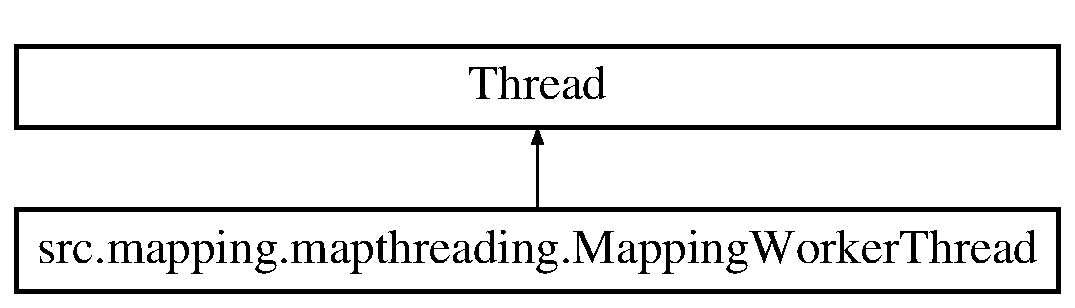
\includegraphics[height=2.000000cm]{classsrc_1_1mapping_1_1mapthreading_1_1_mapping_worker_thread}
\end{center}
\end{figure}
\subsection*{Public Member Functions}
\begin{DoxyCompactItemize}
\item 
def \hyperlink{classsrc_1_1mapping_1_1mapthreading_1_1_mapping_worker_thread_a369abd1822eee49c2a800bf80939ca63}{\+\_\+\+\_\+init\+\_\+\+\_\+} (self, \hyperlink{classsrc_1_1mapping_1_1mapthreading_1_1_mapping_worker_thread_a31a9d651719e7dc0c3c0655885b057f1}{worker\+\_\+id}, \hyperlink{classsrc_1_1mapping_1_1mapthreading_1_1_mapping_worker_thread_a3b681382a138a5eee92f956792f96445}{vector\+\_\+dict}, \hyperlink{classsrc_1_1mapping_1_1mapthreading_1_1_mapping_worker_thread_a64f7aadd3ef3abd74551927eaddad44c}{vector\+\_\+queue}, \hyperlink{classsrc_1_1mapping_1_1mapthreading_1_1_mapping_worker_thread_a9ee70fb431a73f6600fa8d9fcfbb1789}{vector\+\_\+outpath}, \hyperlink{classsrc_1_1mapping_1_1mapthreading_1_1_mapping_worker_thread_aef3a19d93efa561529cd8c119dd64e8d}{features}, \hyperlink{classsrc_1_1mapping_1_1mapthreading_1_1_mapping_worker_thread_a8d87ef19617f8a43ff093a075ddc6f57}{occurrences}, \hyperlink{classsrc_1_1mapping_1_1mapthreading_1_1_mapping_worker_thread_ae26274456128e01544339e9ec7c4eefb}{indices})
\item 
def \hyperlink{classsrc_1_1mapping_1_1mapthreading_1_1_mapping_worker_thread_a212107a8a9d636bb3a24d45fa4246d69}{run} (self)
\item 
def \hyperlink{classsrc_1_1mapping_1_1mapthreading_1_1_mapping_worker_thread_aa77a8323d55e45dcded08d8e685394fc}{distance} (self, v1, v2)
\item 
def \hyperlink{classsrc_1_1mapping_1_1mapthreading_1_1_mapping_worker_thread_a4fb8b9904cf52294558d42c1445e32a8}{euclidian\+\_\+distance1} (self, v1, v2)
\item 
def \hyperlink{classsrc_1_1mapping_1_1mapthreading_1_1_mapping_worker_thread_a66a6db871ae1b09af299153adfa800eb}{euclidian\+\_\+distance2} (self, v1, v2)
\item 
def \hyperlink{classsrc_1_1mapping_1_1mapthreading_1_1_mapping_worker_thread_a1a7bb52cba2f7bb5f498992e1bc0bef3}{manhattan\+\_\+distance} (self, v1, v2)
\item 
def \hyperlink{classsrc_1_1mapping_1_1mapthreading_1_1_mapping_worker_thread_a7dcb7d6ab0262ca2816d51653673e142}{cosine\+\_\+similarity} (self, v1, v2)
\item 
def \hyperlink{classsrc_1_1mapping_1_1mapthreading_1_1_mapping_worker_thread_a0c029daa0905f4a7741759a7ce50f2be}{concat} (self, v1, v2)
\item 
def \hyperlink{classsrc_1_1mapping_1_1mapthreading_1_1_mapping_worker_thread_ab15fd47a94c7a2ed04b3ad3213cf1d34}{spray} (self, v1, v2, cooc)
\item 
def \hyperlink{classsrc_1_1mapping_1_1mapthreading_1_1_mapping_worker_thread_a0fe2472fc7b1bf19687bb1c986419129}{hash\+\_\+indices} (self, i1, i2)
\end{DoxyCompactItemize}
\subsection*{Public Attributes}
\begin{DoxyCompactItemize}
\item 
\hyperlink{classsrc_1_1mapping_1_1mapthreading_1_1_mapping_worker_thread_a31a9d651719e7dc0c3c0655885b057f1}{worker\+\_\+id}
\item 
\hyperlink{classsrc_1_1mapping_1_1mapthreading_1_1_mapping_worker_thread_a3b681382a138a5eee92f956792f96445}{vector\+\_\+dict}
\item 
\hyperlink{classsrc_1_1mapping_1_1mapthreading_1_1_mapping_worker_thread_a8d87ef19617f8a43ff093a075ddc6f57}{occurrences}
\item 
\hyperlink{classsrc_1_1mapping_1_1mapthreading_1_1_mapping_worker_thread_ae26274456128e01544339e9ec7c4eefb}{indices}
\item 
\hyperlink{classsrc_1_1mapping_1_1mapthreading_1_1_mapping_worker_thread_a64f7aadd3ef3abd74551927eaddad44c}{vector\+\_\+queue}
\item 
\hyperlink{classsrc_1_1mapping_1_1mapthreading_1_1_mapping_worker_thread_a9ee70fb431a73f6600fa8d9fcfbb1789}{vector\+\_\+outpath}
\item 
\hyperlink{classsrc_1_1mapping_1_1mapthreading_1_1_mapping_worker_thread_aef3a19d93efa561529cd8c119dd64e8d}{features}
\item 
\hyperlink{classsrc_1_1mapping_1_1mapthreading_1_1_mapping_worker_thread_aef1aaaa9dcac3a85778d52927abfd640}{voperations}
\end{DoxyCompactItemize}


\subsection{Constructor \& Destructor Documentation}
\index{src\+::mapping\+::mapthreading\+::\+Mapping\+Worker\+Thread@{src\+::mapping\+::mapthreading\+::\+Mapping\+Worker\+Thread}!\+\_\+\+\_\+init\+\_\+\+\_\+@{\+\_\+\+\_\+init\+\_\+\+\_\+}}
\index{\+\_\+\+\_\+init\+\_\+\+\_\+@{\+\_\+\+\_\+init\+\_\+\+\_\+}!src\+::mapping\+::mapthreading\+::\+Mapping\+Worker\+Thread@{src\+::mapping\+::mapthreading\+::\+Mapping\+Worker\+Thread}}
\subsubsection[{\texorpdfstring{\+\_\+\+\_\+init\+\_\+\+\_\+(self, worker\+\_\+id, vector\+\_\+dict, vector\+\_\+queue, vector\+\_\+outpath, features, occurrences, indices)}{\_\_init\_\_(self, worker\_id, vector\_dict, vector\_queue, vector\_outpath, features, occurrences, indices)}}]{\setlength{\rightskip}{0pt plus 5cm}def src.\+mapping.\+mapthreading.\+Mapping\+Worker\+Thread.\+\_\+\+\_\+init\+\_\+\+\_\+ (
\begin{DoxyParamCaption}
\item[{}]{self, }
\item[{}]{worker\+\_\+id, }
\item[{}]{vector\+\_\+dict, }
\item[{}]{vector\+\_\+queue, }
\item[{}]{vector\+\_\+outpath, }
\item[{}]{features, }
\item[{}]{occurrences, }
\item[{}]{indices}
\end{DoxyParamCaption}
)}\hypertarget{classsrc_1_1mapping_1_1mapthreading_1_1_mapping_worker_thread_a369abd1822eee49c2a800bf80939ca63}{}\label{classsrc_1_1mapping_1_1mapthreading_1_1_mapping_worker_thread_a369abd1822eee49c2a800bf80939ca63}


\subsection{Member Function Documentation}
\index{src\+::mapping\+::mapthreading\+::\+Mapping\+Worker\+Thread@{src\+::mapping\+::mapthreading\+::\+Mapping\+Worker\+Thread}!concat@{concat}}
\index{concat@{concat}!src\+::mapping\+::mapthreading\+::\+Mapping\+Worker\+Thread@{src\+::mapping\+::mapthreading\+::\+Mapping\+Worker\+Thread}}
\subsubsection[{\texorpdfstring{concat(self, v1, v2)}{concat(self, v1, v2)}}]{\setlength{\rightskip}{0pt plus 5cm}def src.\+mapping.\+mapthreading.\+Mapping\+Worker\+Thread.\+concat (
\begin{DoxyParamCaption}
\item[{}]{self, }
\item[{}]{v1, }
\item[{}]{v2}
\end{DoxyParamCaption}
)}\hypertarget{classsrc_1_1mapping_1_1mapthreading_1_1_mapping_worker_thread_a0c029daa0905f4a7741759a7ce50f2be}{}\label{classsrc_1_1mapping_1_1mapthreading_1_1_mapping_worker_thread_a0c029daa0905f4a7741759a7ce50f2be}
\index{src\+::mapping\+::mapthreading\+::\+Mapping\+Worker\+Thread@{src\+::mapping\+::mapthreading\+::\+Mapping\+Worker\+Thread}!cosine\+\_\+similarity@{cosine\+\_\+similarity}}
\index{cosine\+\_\+similarity@{cosine\+\_\+similarity}!src\+::mapping\+::mapthreading\+::\+Mapping\+Worker\+Thread@{src\+::mapping\+::mapthreading\+::\+Mapping\+Worker\+Thread}}
\subsubsection[{\texorpdfstring{cosine\+\_\+similarity(self, v1, v2)}{cosine\_similarity(self, v1, v2)}}]{\setlength{\rightskip}{0pt plus 5cm}def src.\+mapping.\+mapthreading.\+Mapping\+Worker\+Thread.\+cosine\+\_\+similarity (
\begin{DoxyParamCaption}
\item[{}]{self, }
\item[{}]{v1, }
\item[{}]{v2}
\end{DoxyParamCaption}
)}\hypertarget{classsrc_1_1mapping_1_1mapthreading_1_1_mapping_worker_thread_a7dcb7d6ab0262ca2816d51653673e142}{}\label{classsrc_1_1mapping_1_1mapthreading_1_1_mapping_worker_thread_a7dcb7d6ab0262ca2816d51653673e142}
\index{src\+::mapping\+::mapthreading\+::\+Mapping\+Worker\+Thread@{src\+::mapping\+::mapthreading\+::\+Mapping\+Worker\+Thread}!distance@{distance}}
\index{distance@{distance}!src\+::mapping\+::mapthreading\+::\+Mapping\+Worker\+Thread@{src\+::mapping\+::mapthreading\+::\+Mapping\+Worker\+Thread}}
\subsubsection[{\texorpdfstring{distance(self, v1, v2)}{distance(self, v1, v2)}}]{\setlength{\rightskip}{0pt plus 5cm}def src.\+mapping.\+mapthreading.\+Mapping\+Worker\+Thread.\+distance (
\begin{DoxyParamCaption}
\item[{}]{self, }
\item[{}]{v1, }
\item[{}]{v2}
\end{DoxyParamCaption}
)}\hypertarget{classsrc_1_1mapping_1_1mapthreading_1_1_mapping_worker_thread_aa77a8323d55e45dcded08d8e685394fc}{}\label{classsrc_1_1mapping_1_1mapthreading_1_1_mapping_worker_thread_aa77a8323d55e45dcded08d8e685394fc}
\index{src\+::mapping\+::mapthreading\+::\+Mapping\+Worker\+Thread@{src\+::mapping\+::mapthreading\+::\+Mapping\+Worker\+Thread}!euclidian\+\_\+distance1@{euclidian\+\_\+distance1}}
\index{euclidian\+\_\+distance1@{euclidian\+\_\+distance1}!src\+::mapping\+::mapthreading\+::\+Mapping\+Worker\+Thread@{src\+::mapping\+::mapthreading\+::\+Mapping\+Worker\+Thread}}
\subsubsection[{\texorpdfstring{euclidian\+\_\+distance1(self, v1, v2)}{euclidian\_distance1(self, v1, v2)}}]{\setlength{\rightskip}{0pt plus 5cm}def src.\+mapping.\+mapthreading.\+Mapping\+Worker\+Thread.\+euclidian\+\_\+distance1 (
\begin{DoxyParamCaption}
\item[{}]{self, }
\item[{}]{v1, }
\item[{}]{v2}
\end{DoxyParamCaption}
)}\hypertarget{classsrc_1_1mapping_1_1mapthreading_1_1_mapping_worker_thread_a4fb8b9904cf52294558d42c1445e32a8}{}\label{classsrc_1_1mapping_1_1mapthreading_1_1_mapping_worker_thread_a4fb8b9904cf52294558d42c1445e32a8}
\index{src\+::mapping\+::mapthreading\+::\+Mapping\+Worker\+Thread@{src\+::mapping\+::mapthreading\+::\+Mapping\+Worker\+Thread}!euclidian\+\_\+distance2@{euclidian\+\_\+distance2}}
\index{euclidian\+\_\+distance2@{euclidian\+\_\+distance2}!src\+::mapping\+::mapthreading\+::\+Mapping\+Worker\+Thread@{src\+::mapping\+::mapthreading\+::\+Mapping\+Worker\+Thread}}
\subsubsection[{\texorpdfstring{euclidian\+\_\+distance2(self, v1, v2)}{euclidian\_distance2(self, v1, v2)}}]{\setlength{\rightskip}{0pt plus 5cm}def src.\+mapping.\+mapthreading.\+Mapping\+Worker\+Thread.\+euclidian\+\_\+distance2 (
\begin{DoxyParamCaption}
\item[{}]{self, }
\item[{}]{v1, }
\item[{}]{v2}
\end{DoxyParamCaption}
)}\hypertarget{classsrc_1_1mapping_1_1mapthreading_1_1_mapping_worker_thread_a66a6db871ae1b09af299153adfa800eb}{}\label{classsrc_1_1mapping_1_1mapthreading_1_1_mapping_worker_thread_a66a6db871ae1b09af299153adfa800eb}
\index{src\+::mapping\+::mapthreading\+::\+Mapping\+Worker\+Thread@{src\+::mapping\+::mapthreading\+::\+Mapping\+Worker\+Thread}!hash\+\_\+indices@{hash\+\_\+indices}}
\index{hash\+\_\+indices@{hash\+\_\+indices}!src\+::mapping\+::mapthreading\+::\+Mapping\+Worker\+Thread@{src\+::mapping\+::mapthreading\+::\+Mapping\+Worker\+Thread}}
\subsubsection[{\texorpdfstring{hash\+\_\+indices(self, i1, i2)}{hash\_indices(self, i1, i2)}}]{\setlength{\rightskip}{0pt plus 5cm}def src.\+mapping.\+mapthreading.\+Mapping\+Worker\+Thread.\+hash\+\_\+indices (
\begin{DoxyParamCaption}
\item[{}]{self, }
\item[{}]{i1, }
\item[{}]{i2}
\end{DoxyParamCaption}
)}\hypertarget{classsrc_1_1mapping_1_1mapthreading_1_1_mapping_worker_thread_a0fe2472fc7b1bf19687bb1c986419129}{}\label{classsrc_1_1mapping_1_1mapthreading_1_1_mapping_worker_thread_a0fe2472fc7b1bf19687bb1c986419129}
\index{src\+::mapping\+::mapthreading\+::\+Mapping\+Worker\+Thread@{src\+::mapping\+::mapthreading\+::\+Mapping\+Worker\+Thread}!manhattan\+\_\+distance@{manhattan\+\_\+distance}}
\index{manhattan\+\_\+distance@{manhattan\+\_\+distance}!src\+::mapping\+::mapthreading\+::\+Mapping\+Worker\+Thread@{src\+::mapping\+::mapthreading\+::\+Mapping\+Worker\+Thread}}
\subsubsection[{\texorpdfstring{manhattan\+\_\+distance(self, v1, v2)}{manhattan\_distance(self, v1, v2)}}]{\setlength{\rightskip}{0pt plus 5cm}def src.\+mapping.\+mapthreading.\+Mapping\+Worker\+Thread.\+manhattan\+\_\+distance (
\begin{DoxyParamCaption}
\item[{}]{self, }
\item[{}]{v1, }
\item[{}]{v2}
\end{DoxyParamCaption}
)}\hypertarget{classsrc_1_1mapping_1_1mapthreading_1_1_mapping_worker_thread_a1a7bb52cba2f7bb5f498992e1bc0bef3}{}\label{classsrc_1_1mapping_1_1mapthreading_1_1_mapping_worker_thread_a1a7bb52cba2f7bb5f498992e1bc0bef3}
\index{src\+::mapping\+::mapthreading\+::\+Mapping\+Worker\+Thread@{src\+::mapping\+::mapthreading\+::\+Mapping\+Worker\+Thread}!run@{run}}
\index{run@{run}!src\+::mapping\+::mapthreading\+::\+Mapping\+Worker\+Thread@{src\+::mapping\+::mapthreading\+::\+Mapping\+Worker\+Thread}}
\subsubsection[{\texorpdfstring{run(self)}{run(self)}}]{\setlength{\rightskip}{0pt plus 5cm}def src.\+mapping.\+mapthreading.\+Mapping\+Worker\+Thread.\+run (
\begin{DoxyParamCaption}
\item[{}]{self}
\end{DoxyParamCaption}
)}\hypertarget{classsrc_1_1mapping_1_1mapthreading_1_1_mapping_worker_thread_a212107a8a9d636bb3a24d45fa4246d69}{}\label{classsrc_1_1mapping_1_1mapthreading_1_1_mapping_worker_thread_a212107a8a9d636bb3a24d45fa4246d69}
\index{src\+::mapping\+::mapthreading\+::\+Mapping\+Worker\+Thread@{src\+::mapping\+::mapthreading\+::\+Mapping\+Worker\+Thread}!spray@{spray}}
\index{spray@{spray}!src\+::mapping\+::mapthreading\+::\+Mapping\+Worker\+Thread@{src\+::mapping\+::mapthreading\+::\+Mapping\+Worker\+Thread}}
\subsubsection[{\texorpdfstring{spray(self, v1, v2, cooc)}{spray(self, v1, v2, cooc)}}]{\setlength{\rightskip}{0pt plus 5cm}def src.\+mapping.\+mapthreading.\+Mapping\+Worker\+Thread.\+spray (
\begin{DoxyParamCaption}
\item[{}]{self, }
\item[{}]{v1, }
\item[{}]{v2, }
\item[{}]{cooc}
\end{DoxyParamCaption}
)}\hypertarget{classsrc_1_1mapping_1_1mapthreading_1_1_mapping_worker_thread_ab15fd47a94c7a2ed04b3ad3213cf1d34}{}\label{classsrc_1_1mapping_1_1mapthreading_1_1_mapping_worker_thread_ab15fd47a94c7a2ed04b3ad3213cf1d34}


\subsection{Member Data Documentation}
\index{src\+::mapping\+::mapthreading\+::\+Mapping\+Worker\+Thread@{src\+::mapping\+::mapthreading\+::\+Mapping\+Worker\+Thread}!features@{features}}
\index{features@{features}!src\+::mapping\+::mapthreading\+::\+Mapping\+Worker\+Thread@{src\+::mapping\+::mapthreading\+::\+Mapping\+Worker\+Thread}}
\subsubsection[{\texorpdfstring{features}{features}}]{\setlength{\rightskip}{0pt plus 5cm}src.\+mapping.\+mapthreading.\+Mapping\+Worker\+Thread.\+features}\hypertarget{classsrc_1_1mapping_1_1mapthreading_1_1_mapping_worker_thread_aef3a19d93efa561529cd8c119dd64e8d}{}\label{classsrc_1_1mapping_1_1mapthreading_1_1_mapping_worker_thread_aef3a19d93efa561529cd8c119dd64e8d}
\index{src\+::mapping\+::mapthreading\+::\+Mapping\+Worker\+Thread@{src\+::mapping\+::mapthreading\+::\+Mapping\+Worker\+Thread}!indices@{indices}}
\index{indices@{indices}!src\+::mapping\+::mapthreading\+::\+Mapping\+Worker\+Thread@{src\+::mapping\+::mapthreading\+::\+Mapping\+Worker\+Thread}}
\subsubsection[{\texorpdfstring{indices}{indices}}]{\setlength{\rightskip}{0pt plus 5cm}src.\+mapping.\+mapthreading.\+Mapping\+Worker\+Thread.\+indices}\hypertarget{classsrc_1_1mapping_1_1mapthreading_1_1_mapping_worker_thread_ae26274456128e01544339e9ec7c4eefb}{}\label{classsrc_1_1mapping_1_1mapthreading_1_1_mapping_worker_thread_ae26274456128e01544339e9ec7c4eefb}
\index{src\+::mapping\+::mapthreading\+::\+Mapping\+Worker\+Thread@{src\+::mapping\+::mapthreading\+::\+Mapping\+Worker\+Thread}!occurrences@{occurrences}}
\index{occurrences@{occurrences}!src\+::mapping\+::mapthreading\+::\+Mapping\+Worker\+Thread@{src\+::mapping\+::mapthreading\+::\+Mapping\+Worker\+Thread}}
\subsubsection[{\texorpdfstring{occurrences}{occurrences}}]{\setlength{\rightskip}{0pt plus 5cm}src.\+mapping.\+mapthreading.\+Mapping\+Worker\+Thread.\+occurrences}\hypertarget{classsrc_1_1mapping_1_1mapthreading_1_1_mapping_worker_thread_a8d87ef19617f8a43ff093a075ddc6f57}{}\label{classsrc_1_1mapping_1_1mapthreading_1_1_mapping_worker_thread_a8d87ef19617f8a43ff093a075ddc6f57}
\index{src\+::mapping\+::mapthreading\+::\+Mapping\+Worker\+Thread@{src\+::mapping\+::mapthreading\+::\+Mapping\+Worker\+Thread}!vector\+\_\+dict@{vector\+\_\+dict}}
\index{vector\+\_\+dict@{vector\+\_\+dict}!src\+::mapping\+::mapthreading\+::\+Mapping\+Worker\+Thread@{src\+::mapping\+::mapthreading\+::\+Mapping\+Worker\+Thread}}
\subsubsection[{\texorpdfstring{vector\+\_\+dict}{vector\_dict}}]{\setlength{\rightskip}{0pt plus 5cm}src.\+mapping.\+mapthreading.\+Mapping\+Worker\+Thread.\+vector\+\_\+dict}\hypertarget{classsrc_1_1mapping_1_1mapthreading_1_1_mapping_worker_thread_a3b681382a138a5eee92f956792f96445}{}\label{classsrc_1_1mapping_1_1mapthreading_1_1_mapping_worker_thread_a3b681382a138a5eee92f956792f96445}
\index{src\+::mapping\+::mapthreading\+::\+Mapping\+Worker\+Thread@{src\+::mapping\+::mapthreading\+::\+Mapping\+Worker\+Thread}!vector\+\_\+outpath@{vector\+\_\+outpath}}
\index{vector\+\_\+outpath@{vector\+\_\+outpath}!src\+::mapping\+::mapthreading\+::\+Mapping\+Worker\+Thread@{src\+::mapping\+::mapthreading\+::\+Mapping\+Worker\+Thread}}
\subsubsection[{\texorpdfstring{vector\+\_\+outpath}{vector\_outpath}}]{\setlength{\rightskip}{0pt plus 5cm}src.\+mapping.\+mapthreading.\+Mapping\+Worker\+Thread.\+vector\+\_\+outpath}\hypertarget{classsrc_1_1mapping_1_1mapthreading_1_1_mapping_worker_thread_a9ee70fb431a73f6600fa8d9fcfbb1789}{}\label{classsrc_1_1mapping_1_1mapthreading_1_1_mapping_worker_thread_a9ee70fb431a73f6600fa8d9fcfbb1789}
\index{src\+::mapping\+::mapthreading\+::\+Mapping\+Worker\+Thread@{src\+::mapping\+::mapthreading\+::\+Mapping\+Worker\+Thread}!vector\+\_\+queue@{vector\+\_\+queue}}
\index{vector\+\_\+queue@{vector\+\_\+queue}!src\+::mapping\+::mapthreading\+::\+Mapping\+Worker\+Thread@{src\+::mapping\+::mapthreading\+::\+Mapping\+Worker\+Thread}}
\subsubsection[{\texorpdfstring{vector\+\_\+queue}{vector\_queue}}]{\setlength{\rightskip}{0pt plus 5cm}src.\+mapping.\+mapthreading.\+Mapping\+Worker\+Thread.\+vector\+\_\+queue}\hypertarget{classsrc_1_1mapping_1_1mapthreading_1_1_mapping_worker_thread_a64f7aadd3ef3abd74551927eaddad44c}{}\label{classsrc_1_1mapping_1_1mapthreading_1_1_mapping_worker_thread_a64f7aadd3ef3abd74551927eaddad44c}
\index{src\+::mapping\+::mapthreading\+::\+Mapping\+Worker\+Thread@{src\+::mapping\+::mapthreading\+::\+Mapping\+Worker\+Thread}!voperations@{voperations}}
\index{voperations@{voperations}!src\+::mapping\+::mapthreading\+::\+Mapping\+Worker\+Thread@{src\+::mapping\+::mapthreading\+::\+Mapping\+Worker\+Thread}}
\subsubsection[{\texorpdfstring{voperations}{voperations}}]{\setlength{\rightskip}{0pt plus 5cm}src.\+mapping.\+mapthreading.\+Mapping\+Worker\+Thread.\+voperations}\hypertarget{classsrc_1_1mapping_1_1mapthreading_1_1_mapping_worker_thread_aef1aaaa9dcac3a85778d52927abfd640}{}\label{classsrc_1_1mapping_1_1mapthreading_1_1_mapping_worker_thread_aef1aaaa9dcac3a85778d52927abfd640}
\index{src\+::mapping\+::mapthreading\+::\+Mapping\+Worker\+Thread@{src\+::mapping\+::mapthreading\+::\+Mapping\+Worker\+Thread}!worker\+\_\+id@{worker\+\_\+id}}
\index{worker\+\_\+id@{worker\+\_\+id}!src\+::mapping\+::mapthreading\+::\+Mapping\+Worker\+Thread@{src\+::mapping\+::mapthreading\+::\+Mapping\+Worker\+Thread}}
\subsubsection[{\texorpdfstring{worker\+\_\+id}{worker\_id}}]{\setlength{\rightskip}{0pt plus 5cm}src.\+mapping.\+mapthreading.\+Mapping\+Worker\+Thread.\+worker\+\_\+id}\hypertarget{classsrc_1_1mapping_1_1mapthreading_1_1_mapping_worker_thread_a31a9d651719e7dc0c3c0655885b057f1}{}\label{classsrc_1_1mapping_1_1mapthreading_1_1_mapping_worker_thread_a31a9d651719e7dc0c3c0655885b057f1}


The documentation for this class was generated from the following file\+:\begin{DoxyCompactItemize}
\item 
/\+Users/dennisulmer/\+Documents/\+Studium/7. Semester/\+Computerlinguistik/\+Bachelorarbeit/src/mapping/\hyperlink{mapthreading_8py}{mapthreading.\+py}\end{DoxyCompactItemize}

\hypertarget{classsrc_1_1prep_1_1relations_1_1relations_1_1_missing_translation_exception}{}\section{src.\+prep.\+relations.\+relations.\+Missing\+Translation\+Exception Class Reference}
\label{classsrc_1_1prep_1_1relations_1_1relations_1_1_missing_translation_exception}\index{src.\+prep.\+relations.\+relations.\+Missing\+Translation\+Exception@{src.\+prep.\+relations.\+relations.\+Missing\+Translation\+Exception}}
Inheritance diagram for src.\+prep.\+relations.\+relations.\+Missing\+Translation\+Exception\+:\begin{figure}[H]
\begin{center}
\leavevmode
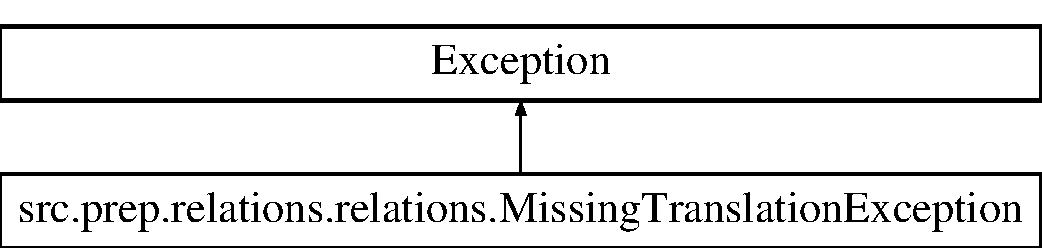
\includegraphics[height=2.000000cm]{classsrc_1_1prep_1_1relations_1_1relations_1_1_missing_translation_exception}
\end{center}
\end{figure}
\subsection*{Public Member Functions}
\begin{DoxyCompactItemize}
\item 
def \hyperlink{classsrc_1_1prep_1_1relations_1_1relations_1_1_missing_translation_exception_a8c209afdb46688cf5fe1da6a5f0bef02}{get\+\_\+id} (self)
\end{DoxyCompactItemize}


\subsection{Member Function Documentation}
\index{src\+::prep\+::relations\+::relations\+::\+Missing\+Translation\+Exception@{src\+::prep\+::relations\+::relations\+::\+Missing\+Translation\+Exception}!get\+\_\+id@{get\+\_\+id}}
\index{get\+\_\+id@{get\+\_\+id}!src\+::prep\+::relations\+::relations\+::\+Missing\+Translation\+Exception@{src\+::prep\+::relations\+::relations\+::\+Missing\+Translation\+Exception}}
\subsubsection[{\texorpdfstring{get\+\_\+id(self)}{get\_id(self)}}]{\setlength{\rightskip}{0pt plus 5cm}def src.\+prep.\+relations.\+relations.\+Missing\+Translation\+Exception.\+get\+\_\+id (
\begin{DoxyParamCaption}
\item[{}]{self}
\end{DoxyParamCaption}
)}\hypertarget{classsrc_1_1prep_1_1relations_1_1relations_1_1_missing_translation_exception_a8c209afdb46688cf5fe1da6a5f0bef02}{}\label{classsrc_1_1prep_1_1relations_1_1relations_1_1_missing_translation_exception_a8c209afdb46688cf5fe1da6a5f0bef02}


The documentation for this class was generated from the following file\+:\begin{DoxyCompactItemize}
\item 
/\+Users/dennisulmer/\+Documents/\+Studium/7. Semester/\+Computerlinguistik/\+Bachelorarbeit/src/prep/relations/\hyperlink{relations_8py}{relations.\+py}\end{DoxyCompactItemize}

\hypertarget{classsrc_1_1mapping_1_1mapthreading_1_1_vector_dict}{}\section{src.\+mapping.\+mapthreading.\+Vector\+Dict Class Reference}
\label{classsrc_1_1mapping_1_1mapthreading_1_1_vector_dict}\index{src.\+mapping.\+mapthreading.\+Vector\+Dict@{src.\+mapping.\+mapthreading.\+Vector\+Dict}}
Inheritance diagram for src.\+mapping.\+mapthreading.\+Vector\+Dict\+:\begin{figure}[H]
\begin{center}
\leavevmode
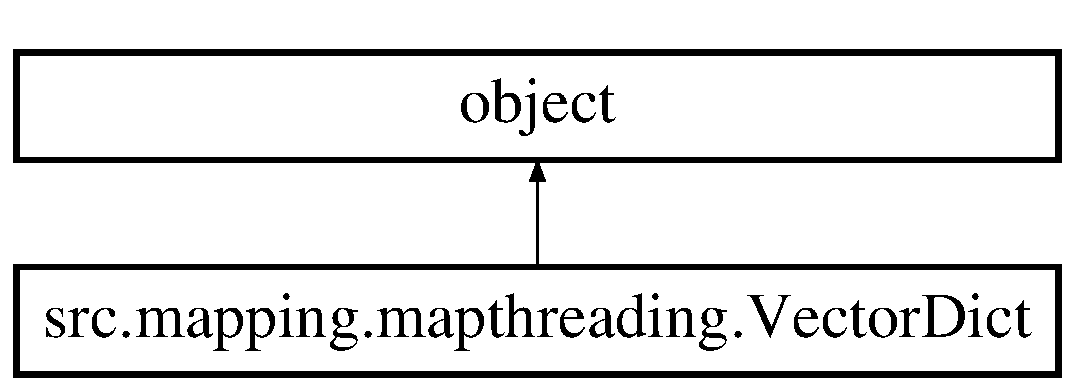
\includegraphics[height=2.000000cm]{classsrc_1_1mapping_1_1mapthreading_1_1_vector_dict}
\end{center}
\end{figure}
\subsection*{Public Member Functions}
\begin{DoxyCompactItemize}
\item 
def \hyperlink{classsrc_1_1mapping_1_1mapthreading_1_1_vector_dict_a327fffd77dee4ed0d26e912acf1c6ff1}{\+\_\+\+\_\+init\+\_\+\+\_\+} (self)
\item 
def \hyperlink{classsrc_1_1mapping_1_1mapthreading_1_1_vector_dict_a0deaf97f89e5be6de28191a387dd1fd3}{get\+\_\+vector} (self, index)
\item 
def \hyperlink{classsrc_1_1mapping_1_1mapthreading_1_1_vector_dict_a117a9d830431bdd71fe6fcb426f30f9d}{add\+\_\+vector} (self, index, vector)
\item 
def \hyperlink{classsrc_1_1mapping_1_1mapthreading_1_1_vector_dict_aebca32a6845dbfd9162e29e31bd7e506}{add\+\_\+skippable} (self, index)
\item 
def \hyperlink{classsrc_1_1mapping_1_1mapthreading_1_1_vector_dict_a3bab8d126803065aa768519341ab54e2}{get\+\_\+keys} (self)
\item 
def \hyperlink{classsrc_1_1mapping_1_1mapthreading_1_1_vector_dict_a2099b39b18452554de35416ea569ee2e}{skippable} (self, index\+\_\+hash)
\end{DoxyCompactItemize}
\subsection*{Public Attributes}
\begin{DoxyCompactItemize}
\item 
\hyperlink{classsrc_1_1mapping_1_1mapthreading_1_1_vector_dict_a3541d1410985f5b531d7f6c7f67cf2d1}{core\+\_\+dict}
\item 
\hyperlink{classsrc_1_1mapping_1_1mapthreading_1_1_vector_dict_a3ae6f68fd91c50673ace06d486234bfe}{lock}
\item 
\hyperlink{classsrc_1_1mapping_1_1mapthreading_1_1_vector_dict_a6f71fefdbf2c8c31e99190ddd408f558}{skippables}
\end{DoxyCompactItemize}


\subsection{Constructor \& Destructor Documentation}
\index{src\+::mapping\+::mapthreading\+::\+Vector\+Dict@{src\+::mapping\+::mapthreading\+::\+Vector\+Dict}!\+\_\+\+\_\+init\+\_\+\+\_\+@{\+\_\+\+\_\+init\+\_\+\+\_\+}}
\index{\+\_\+\+\_\+init\+\_\+\+\_\+@{\+\_\+\+\_\+init\+\_\+\+\_\+}!src\+::mapping\+::mapthreading\+::\+Vector\+Dict@{src\+::mapping\+::mapthreading\+::\+Vector\+Dict}}
\subsubsection[{\texorpdfstring{\+\_\+\+\_\+init\+\_\+\+\_\+(self)}{\_\_init\_\_(self)}}]{\setlength{\rightskip}{0pt plus 5cm}def src.\+mapping.\+mapthreading.\+Vector\+Dict.\+\_\+\+\_\+init\+\_\+\+\_\+ (
\begin{DoxyParamCaption}
\item[{}]{self}
\end{DoxyParamCaption}
)}\hypertarget{classsrc_1_1mapping_1_1mapthreading_1_1_vector_dict_a327fffd77dee4ed0d26e912acf1c6ff1}{}\label{classsrc_1_1mapping_1_1mapthreading_1_1_vector_dict_a327fffd77dee4ed0d26e912acf1c6ff1}


\subsection{Member Function Documentation}
\index{src\+::mapping\+::mapthreading\+::\+Vector\+Dict@{src\+::mapping\+::mapthreading\+::\+Vector\+Dict}!add\+\_\+skippable@{add\+\_\+skippable}}
\index{add\+\_\+skippable@{add\+\_\+skippable}!src\+::mapping\+::mapthreading\+::\+Vector\+Dict@{src\+::mapping\+::mapthreading\+::\+Vector\+Dict}}
\subsubsection[{\texorpdfstring{add\+\_\+skippable(self, index)}{add\_skippable(self, index)}}]{\setlength{\rightskip}{0pt plus 5cm}def src.\+mapping.\+mapthreading.\+Vector\+Dict.\+add\+\_\+skippable (
\begin{DoxyParamCaption}
\item[{}]{self, }
\item[{}]{index}
\end{DoxyParamCaption}
)}\hypertarget{classsrc_1_1mapping_1_1mapthreading_1_1_vector_dict_aebca32a6845dbfd9162e29e31bd7e506}{}\label{classsrc_1_1mapping_1_1mapthreading_1_1_vector_dict_aebca32a6845dbfd9162e29e31bd7e506}
\index{src\+::mapping\+::mapthreading\+::\+Vector\+Dict@{src\+::mapping\+::mapthreading\+::\+Vector\+Dict}!add\+\_\+vector@{add\+\_\+vector}}
\index{add\+\_\+vector@{add\+\_\+vector}!src\+::mapping\+::mapthreading\+::\+Vector\+Dict@{src\+::mapping\+::mapthreading\+::\+Vector\+Dict}}
\subsubsection[{\texorpdfstring{add\+\_\+vector(self, index, vector)}{add\_vector(self, index, vector)}}]{\setlength{\rightskip}{0pt plus 5cm}def src.\+mapping.\+mapthreading.\+Vector\+Dict.\+add\+\_\+vector (
\begin{DoxyParamCaption}
\item[{}]{self, }
\item[{}]{index, }
\item[{}]{vector}
\end{DoxyParamCaption}
)}\hypertarget{classsrc_1_1mapping_1_1mapthreading_1_1_vector_dict_a117a9d830431bdd71fe6fcb426f30f9d}{}\label{classsrc_1_1mapping_1_1mapthreading_1_1_vector_dict_a117a9d830431bdd71fe6fcb426f30f9d}
\index{src\+::mapping\+::mapthreading\+::\+Vector\+Dict@{src\+::mapping\+::mapthreading\+::\+Vector\+Dict}!get\+\_\+keys@{get\+\_\+keys}}
\index{get\+\_\+keys@{get\+\_\+keys}!src\+::mapping\+::mapthreading\+::\+Vector\+Dict@{src\+::mapping\+::mapthreading\+::\+Vector\+Dict}}
\subsubsection[{\texorpdfstring{get\+\_\+keys(self)}{get\_keys(self)}}]{\setlength{\rightskip}{0pt plus 5cm}def src.\+mapping.\+mapthreading.\+Vector\+Dict.\+get\+\_\+keys (
\begin{DoxyParamCaption}
\item[{}]{self}
\end{DoxyParamCaption}
)}\hypertarget{classsrc_1_1mapping_1_1mapthreading_1_1_vector_dict_a3bab8d126803065aa768519341ab54e2}{}\label{classsrc_1_1mapping_1_1mapthreading_1_1_vector_dict_a3bab8d126803065aa768519341ab54e2}
\index{src\+::mapping\+::mapthreading\+::\+Vector\+Dict@{src\+::mapping\+::mapthreading\+::\+Vector\+Dict}!get\+\_\+vector@{get\+\_\+vector}}
\index{get\+\_\+vector@{get\+\_\+vector}!src\+::mapping\+::mapthreading\+::\+Vector\+Dict@{src\+::mapping\+::mapthreading\+::\+Vector\+Dict}}
\subsubsection[{\texorpdfstring{get\+\_\+vector(self, index)}{get\_vector(self, index)}}]{\setlength{\rightskip}{0pt plus 5cm}def src.\+mapping.\+mapthreading.\+Vector\+Dict.\+get\+\_\+vector (
\begin{DoxyParamCaption}
\item[{}]{self, }
\item[{}]{index}
\end{DoxyParamCaption}
)}\hypertarget{classsrc_1_1mapping_1_1mapthreading_1_1_vector_dict_a0deaf97f89e5be6de28191a387dd1fd3}{}\label{classsrc_1_1mapping_1_1mapthreading_1_1_vector_dict_a0deaf97f89e5be6de28191a387dd1fd3}
\index{src\+::mapping\+::mapthreading\+::\+Vector\+Dict@{src\+::mapping\+::mapthreading\+::\+Vector\+Dict}!skippable@{skippable}}
\index{skippable@{skippable}!src\+::mapping\+::mapthreading\+::\+Vector\+Dict@{src\+::mapping\+::mapthreading\+::\+Vector\+Dict}}
\subsubsection[{\texorpdfstring{skippable(self, index\+\_\+hash)}{skippable(self, index\_hash)}}]{\setlength{\rightskip}{0pt plus 5cm}def src.\+mapping.\+mapthreading.\+Vector\+Dict.\+skippable (
\begin{DoxyParamCaption}
\item[{}]{self, }
\item[{}]{index\+\_\+hash}
\end{DoxyParamCaption}
)}\hypertarget{classsrc_1_1mapping_1_1mapthreading_1_1_vector_dict_a2099b39b18452554de35416ea569ee2e}{}\label{classsrc_1_1mapping_1_1mapthreading_1_1_vector_dict_a2099b39b18452554de35416ea569ee2e}


\subsection{Member Data Documentation}
\index{src\+::mapping\+::mapthreading\+::\+Vector\+Dict@{src\+::mapping\+::mapthreading\+::\+Vector\+Dict}!core\+\_\+dict@{core\+\_\+dict}}
\index{core\+\_\+dict@{core\+\_\+dict}!src\+::mapping\+::mapthreading\+::\+Vector\+Dict@{src\+::mapping\+::mapthreading\+::\+Vector\+Dict}}
\subsubsection[{\texorpdfstring{core\+\_\+dict}{core\_dict}}]{\setlength{\rightskip}{0pt plus 5cm}src.\+mapping.\+mapthreading.\+Vector\+Dict.\+core\+\_\+dict}\hypertarget{classsrc_1_1mapping_1_1mapthreading_1_1_vector_dict_a3541d1410985f5b531d7f6c7f67cf2d1}{}\label{classsrc_1_1mapping_1_1mapthreading_1_1_vector_dict_a3541d1410985f5b531d7f6c7f67cf2d1}
\index{src\+::mapping\+::mapthreading\+::\+Vector\+Dict@{src\+::mapping\+::mapthreading\+::\+Vector\+Dict}!lock@{lock}}
\index{lock@{lock}!src\+::mapping\+::mapthreading\+::\+Vector\+Dict@{src\+::mapping\+::mapthreading\+::\+Vector\+Dict}}
\subsubsection[{\texorpdfstring{lock}{lock}}]{\setlength{\rightskip}{0pt plus 5cm}src.\+mapping.\+mapthreading.\+Vector\+Dict.\+lock}\hypertarget{classsrc_1_1mapping_1_1mapthreading_1_1_vector_dict_a3ae6f68fd91c50673ace06d486234bfe}{}\label{classsrc_1_1mapping_1_1mapthreading_1_1_vector_dict_a3ae6f68fd91c50673ace06d486234bfe}
\index{src\+::mapping\+::mapthreading\+::\+Vector\+Dict@{src\+::mapping\+::mapthreading\+::\+Vector\+Dict}!skippables@{skippables}}
\index{skippables@{skippables}!src\+::mapping\+::mapthreading\+::\+Vector\+Dict@{src\+::mapping\+::mapthreading\+::\+Vector\+Dict}}
\subsubsection[{\texorpdfstring{skippables}{skippables}}]{\setlength{\rightskip}{0pt plus 5cm}src.\+mapping.\+mapthreading.\+Vector\+Dict.\+skippables}\hypertarget{classsrc_1_1mapping_1_1mapthreading_1_1_vector_dict_a6f71fefdbf2c8c31e99190ddd408f558}{}\label{classsrc_1_1mapping_1_1mapthreading_1_1_vector_dict_a6f71fefdbf2c8c31e99190ddd408f558}


The documentation for this class was generated from the following file\+:\begin{DoxyCompactItemize}
\item 
/\+Users/dennisulmer/\+Documents/\+Studium/7. Semester/\+Computerlinguistik/\+Bachelorarbeit/src/mapping/\hyperlink{mapthreading_8py}{mapthreading.\+py}\end{DoxyCompactItemize}

\hypertarget{classsrc_1_1eval_1_1word__similarity_1_1_word_sim_master_thread}{}\section{src.\+eval.\+word\+\_\+similarity.\+Word\+Sim\+Master\+Thread Class Reference}
\label{classsrc_1_1eval_1_1word__similarity_1_1_word_sim_master_thread}\index{src.\+eval.\+word\+\_\+similarity.\+Word\+Sim\+Master\+Thread@{src.\+eval.\+word\+\_\+similarity.\+Word\+Sim\+Master\+Thread}}
Inheritance diagram for src.\+eval.\+word\+\_\+similarity.\+Word\+Sim\+Master\+Thread\+:\begin{figure}[H]
\begin{center}
\leavevmode
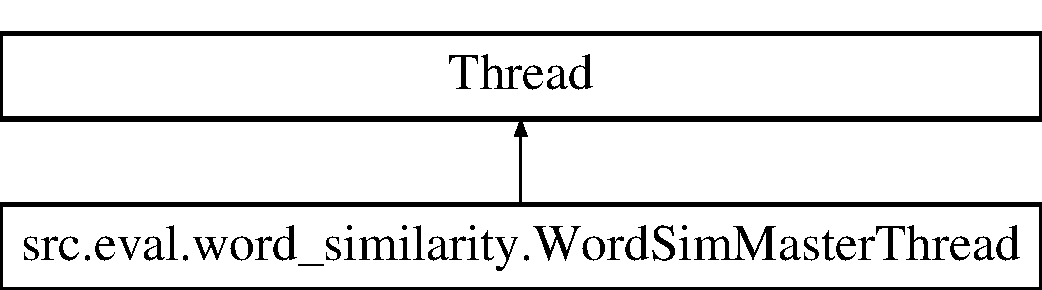
\includegraphics[height=2.000000cm]{classsrc_1_1eval_1_1word__similarity_1_1_word_sim_master_thread}
\end{center}
\end{figure}
\subsection*{Public Member Functions}
\begin{DoxyCompactItemize}
\item 
def \hyperlink{classsrc_1_1eval_1_1word__similarity_1_1_word_sim_master_thread_ab907f7108ed7e9eff1ba25d8381b03cf}{\+\_\+\+\_\+init\+\_\+\+\_\+} (self, \hyperlink{classsrc_1_1eval_1_1word__similarity_1_1_word_sim_master_thread_a2a61f1955df699b96e3d81dd5359d6f9}{n}, \hyperlink{classsrc_1_1eval_1_1word__similarity_1_1_word_sim_master_thread_ab8cddb103eb1085ebe7905ea6f1ef850}{vector\+\_\+inpath}, \hyperlink{classsrc_1_1eval_1_1word__similarity_1_1_word_sim_master_thread_a1322d5a0ef82c1b69d2cbf4b2f2bb9b0}{wordpair\+\_\+inpath}, \hyperlink{classsrc_1_1eval_1_1word__similarity_1_1_word_sim_master_thread_a3ea3cf72df7f131c3fdd3f55255a97ea}{logpath}, \hyperlink{classsrc_1_1eval_1_1word__similarity_1_1_word_sim_master_thread_a7b9dd6657a3b02d0b2e4e81491179721}{format})
\item 
def \hyperlink{classsrc_1_1eval_1_1word__similarity_1_1_word_sim_master_thread_ace5f55f9accb229fb3200b597e7ee942}{start\+\_\+threads} (self)
\item 
def \hyperlink{classsrc_1_1eval_1_1word__similarity_1_1_word_sim_master_thread_a2c133cae966059ffc9da2269111d310b}{prepare} (self)
\item 
def \hyperlink{classsrc_1_1eval_1_1word__similarity_1_1_word_sim_master_thread_ae6d2f50fc627c37fc7b386be592a258c}{remove\+\_\+unknowns} (self)
\end{DoxyCompactItemize}
\subsection*{Public Attributes}
\begin{DoxyCompactItemize}
\item 
\hyperlink{classsrc_1_1eval_1_1word__similarity_1_1_word_sim_master_thread_a2a61f1955df699b96e3d81dd5359d6f9}{n}
\item 
\hyperlink{classsrc_1_1eval_1_1word__similarity_1_1_word_sim_master_thread_ab8cddb103eb1085ebe7905ea6f1ef850}{vector\+\_\+inpath}
\item 
\hyperlink{classsrc_1_1eval_1_1word__similarity_1_1_word_sim_master_thread_a1322d5a0ef82c1b69d2cbf4b2f2bb9b0}{wordpair\+\_\+inpath}
\item 
\hyperlink{classsrc_1_1eval_1_1word__similarity_1_1_word_sim_master_thread_a3ea3cf72df7f131c3fdd3f55255a97ea}{logpath}
\item 
\hyperlink{classsrc_1_1eval_1_1word__similarity_1_1_word_sim_master_thread_a7b9dd6657a3b02d0b2e4e81491179721}{format}
\item 
\hyperlink{classsrc_1_1eval_1_1word__similarity_1_1_word_sim_master_thread_a59eac2f3cbe15c361e88cb64c6ee3296}{model}
\item 
\hyperlink{classsrc_1_1eval_1_1word__similarity_1_1_word_sim_master_thread_afbf0a3906f1ba3ffe6f545c968d3ae1b}{pairs}
\item 
\hyperlink{classsrc_1_1eval_1_1word__similarity_1_1_word_sim_master_thread_abfec0653260234f16e22e15c689a168f}{x}
\item 
\hyperlink{classsrc_1_1eval_1_1word__similarity_1_1_word_sim_master_thread_ae1722e9d60c02419eb0c493592761d10}{y}
\item 
\hyperlink{classsrc_1_1eval_1_1word__similarity_1_1_word_sim_master_thread_a3f91e4211ec9b99e2cbaa67389e9c098}{global\+\_\+error\+\_\+count}
\item 
\hyperlink{classsrc_1_1eval_1_1word__similarity_1_1_word_sim_master_thread_ad5e91c785be6ca4909c7a154afc1a031}{threads}
\item 
\hyperlink{classsrc_1_1eval_1_1word__similarity_1_1_word_sim_master_thread_a8539ca8727131e7d9b2707e8ed4bd03b}{pair\+\_\+queue}
\end{DoxyCompactItemize}


\subsection{Constructor \& Destructor Documentation}
\index{src\+::eval\+::word\+\_\+similarity\+::\+Word\+Sim\+Master\+Thread@{src\+::eval\+::word\+\_\+similarity\+::\+Word\+Sim\+Master\+Thread}!\+\_\+\+\_\+init\+\_\+\+\_\+@{\+\_\+\+\_\+init\+\_\+\+\_\+}}
\index{\+\_\+\+\_\+init\+\_\+\+\_\+@{\+\_\+\+\_\+init\+\_\+\+\_\+}!src\+::eval\+::word\+\_\+similarity\+::\+Word\+Sim\+Master\+Thread@{src\+::eval\+::word\+\_\+similarity\+::\+Word\+Sim\+Master\+Thread}}
\subsubsection[{\texorpdfstring{\+\_\+\+\_\+init\+\_\+\+\_\+(self, n, vector\+\_\+inpath, wordpair\+\_\+inpath, logpath, format)}{\_\_init\_\_(self, n, vector\_inpath, wordpair\_inpath, logpath, format)}}]{\setlength{\rightskip}{0pt plus 5cm}def src.\+eval.\+word\+\_\+similarity.\+Word\+Sim\+Master\+Thread.\+\_\+\+\_\+init\+\_\+\+\_\+ (
\begin{DoxyParamCaption}
\item[{}]{self, }
\item[{}]{n, }
\item[{}]{vector\+\_\+inpath, }
\item[{}]{wordpair\+\_\+inpath, }
\item[{}]{logpath, }
\item[{}]{format}
\end{DoxyParamCaption}
)}\hypertarget{classsrc_1_1eval_1_1word__similarity_1_1_word_sim_master_thread_ab907f7108ed7e9eff1ba25d8381b03cf}{}\label{classsrc_1_1eval_1_1word__similarity_1_1_word_sim_master_thread_ab907f7108ed7e9eff1ba25d8381b03cf}


\subsection{Member Function Documentation}
\index{src\+::eval\+::word\+\_\+similarity\+::\+Word\+Sim\+Master\+Thread@{src\+::eval\+::word\+\_\+similarity\+::\+Word\+Sim\+Master\+Thread}!prepare@{prepare}}
\index{prepare@{prepare}!src\+::eval\+::word\+\_\+similarity\+::\+Word\+Sim\+Master\+Thread@{src\+::eval\+::word\+\_\+similarity\+::\+Word\+Sim\+Master\+Thread}}
\subsubsection[{\texorpdfstring{prepare(self)}{prepare(self)}}]{\setlength{\rightskip}{0pt plus 5cm}def src.\+eval.\+word\+\_\+similarity.\+Word\+Sim\+Master\+Thread.\+prepare (
\begin{DoxyParamCaption}
\item[{}]{self}
\end{DoxyParamCaption}
)}\hypertarget{classsrc_1_1eval_1_1word__similarity_1_1_word_sim_master_thread_a2c133cae966059ffc9da2269111d310b}{}\label{classsrc_1_1eval_1_1word__similarity_1_1_word_sim_master_thread_a2c133cae966059ffc9da2269111d310b}
\index{src\+::eval\+::word\+\_\+similarity\+::\+Word\+Sim\+Master\+Thread@{src\+::eval\+::word\+\_\+similarity\+::\+Word\+Sim\+Master\+Thread}!remove\+\_\+unknowns@{remove\+\_\+unknowns}}
\index{remove\+\_\+unknowns@{remove\+\_\+unknowns}!src\+::eval\+::word\+\_\+similarity\+::\+Word\+Sim\+Master\+Thread@{src\+::eval\+::word\+\_\+similarity\+::\+Word\+Sim\+Master\+Thread}}
\subsubsection[{\texorpdfstring{remove\+\_\+unknowns(self)}{remove\_unknowns(self)}}]{\setlength{\rightskip}{0pt plus 5cm}def src.\+eval.\+word\+\_\+similarity.\+Word\+Sim\+Master\+Thread.\+remove\+\_\+unknowns (
\begin{DoxyParamCaption}
\item[{}]{self}
\end{DoxyParamCaption}
)}\hypertarget{classsrc_1_1eval_1_1word__similarity_1_1_word_sim_master_thread_ae6d2f50fc627c37fc7b386be592a258c}{}\label{classsrc_1_1eval_1_1word__similarity_1_1_word_sim_master_thread_ae6d2f50fc627c37fc7b386be592a258c}
\index{src\+::eval\+::word\+\_\+similarity\+::\+Word\+Sim\+Master\+Thread@{src\+::eval\+::word\+\_\+similarity\+::\+Word\+Sim\+Master\+Thread}!start\+\_\+threads@{start\+\_\+threads}}
\index{start\+\_\+threads@{start\+\_\+threads}!src\+::eval\+::word\+\_\+similarity\+::\+Word\+Sim\+Master\+Thread@{src\+::eval\+::word\+\_\+similarity\+::\+Word\+Sim\+Master\+Thread}}
\subsubsection[{\texorpdfstring{start\+\_\+threads(self)}{start\_threads(self)}}]{\setlength{\rightskip}{0pt plus 5cm}def src.\+eval.\+word\+\_\+similarity.\+Word\+Sim\+Master\+Thread.\+start\+\_\+threads (
\begin{DoxyParamCaption}
\item[{}]{self}
\end{DoxyParamCaption}
)}\hypertarget{classsrc_1_1eval_1_1word__similarity_1_1_word_sim_master_thread_ace5f55f9accb229fb3200b597e7ee942}{}\label{classsrc_1_1eval_1_1word__similarity_1_1_word_sim_master_thread_ace5f55f9accb229fb3200b597e7ee942}


\subsection{Member Data Documentation}
\index{src\+::eval\+::word\+\_\+similarity\+::\+Word\+Sim\+Master\+Thread@{src\+::eval\+::word\+\_\+similarity\+::\+Word\+Sim\+Master\+Thread}!format@{format}}
\index{format@{format}!src\+::eval\+::word\+\_\+similarity\+::\+Word\+Sim\+Master\+Thread@{src\+::eval\+::word\+\_\+similarity\+::\+Word\+Sim\+Master\+Thread}}
\subsubsection[{\texorpdfstring{format}{format}}]{\setlength{\rightskip}{0pt plus 5cm}src.\+eval.\+word\+\_\+similarity.\+Word\+Sim\+Master\+Thread.\+format}\hypertarget{classsrc_1_1eval_1_1word__similarity_1_1_word_sim_master_thread_a7b9dd6657a3b02d0b2e4e81491179721}{}\label{classsrc_1_1eval_1_1word__similarity_1_1_word_sim_master_thread_a7b9dd6657a3b02d0b2e4e81491179721}
\index{src\+::eval\+::word\+\_\+similarity\+::\+Word\+Sim\+Master\+Thread@{src\+::eval\+::word\+\_\+similarity\+::\+Word\+Sim\+Master\+Thread}!global\+\_\+error\+\_\+count@{global\+\_\+error\+\_\+count}}
\index{global\+\_\+error\+\_\+count@{global\+\_\+error\+\_\+count}!src\+::eval\+::word\+\_\+similarity\+::\+Word\+Sim\+Master\+Thread@{src\+::eval\+::word\+\_\+similarity\+::\+Word\+Sim\+Master\+Thread}}
\subsubsection[{\texorpdfstring{global\+\_\+error\+\_\+count}{global\_error\_count}}]{\setlength{\rightskip}{0pt plus 5cm}src.\+eval.\+word\+\_\+similarity.\+Word\+Sim\+Master\+Thread.\+global\+\_\+error\+\_\+count}\hypertarget{classsrc_1_1eval_1_1word__similarity_1_1_word_sim_master_thread_a3f91e4211ec9b99e2cbaa67389e9c098}{}\label{classsrc_1_1eval_1_1word__similarity_1_1_word_sim_master_thread_a3f91e4211ec9b99e2cbaa67389e9c098}
\index{src\+::eval\+::word\+\_\+similarity\+::\+Word\+Sim\+Master\+Thread@{src\+::eval\+::word\+\_\+similarity\+::\+Word\+Sim\+Master\+Thread}!logpath@{logpath}}
\index{logpath@{logpath}!src\+::eval\+::word\+\_\+similarity\+::\+Word\+Sim\+Master\+Thread@{src\+::eval\+::word\+\_\+similarity\+::\+Word\+Sim\+Master\+Thread}}
\subsubsection[{\texorpdfstring{logpath}{logpath}}]{\setlength{\rightskip}{0pt plus 5cm}src.\+eval.\+word\+\_\+similarity.\+Word\+Sim\+Master\+Thread.\+logpath}\hypertarget{classsrc_1_1eval_1_1word__similarity_1_1_word_sim_master_thread_a3ea3cf72df7f131c3fdd3f55255a97ea}{}\label{classsrc_1_1eval_1_1word__similarity_1_1_word_sim_master_thread_a3ea3cf72df7f131c3fdd3f55255a97ea}
\index{src\+::eval\+::word\+\_\+similarity\+::\+Word\+Sim\+Master\+Thread@{src\+::eval\+::word\+\_\+similarity\+::\+Word\+Sim\+Master\+Thread}!model@{model}}
\index{model@{model}!src\+::eval\+::word\+\_\+similarity\+::\+Word\+Sim\+Master\+Thread@{src\+::eval\+::word\+\_\+similarity\+::\+Word\+Sim\+Master\+Thread}}
\subsubsection[{\texorpdfstring{model}{model}}]{\setlength{\rightskip}{0pt plus 5cm}src.\+eval.\+word\+\_\+similarity.\+Word\+Sim\+Master\+Thread.\+model}\hypertarget{classsrc_1_1eval_1_1word__similarity_1_1_word_sim_master_thread_a59eac2f3cbe15c361e88cb64c6ee3296}{}\label{classsrc_1_1eval_1_1word__similarity_1_1_word_sim_master_thread_a59eac2f3cbe15c361e88cb64c6ee3296}
\index{src\+::eval\+::word\+\_\+similarity\+::\+Word\+Sim\+Master\+Thread@{src\+::eval\+::word\+\_\+similarity\+::\+Word\+Sim\+Master\+Thread}!n@{n}}
\index{n@{n}!src\+::eval\+::word\+\_\+similarity\+::\+Word\+Sim\+Master\+Thread@{src\+::eval\+::word\+\_\+similarity\+::\+Word\+Sim\+Master\+Thread}}
\subsubsection[{\texorpdfstring{n}{n}}]{\setlength{\rightskip}{0pt plus 5cm}src.\+eval.\+word\+\_\+similarity.\+Word\+Sim\+Master\+Thread.\+n}\hypertarget{classsrc_1_1eval_1_1word__similarity_1_1_word_sim_master_thread_a2a61f1955df699b96e3d81dd5359d6f9}{}\label{classsrc_1_1eval_1_1word__similarity_1_1_word_sim_master_thread_a2a61f1955df699b96e3d81dd5359d6f9}
\index{src\+::eval\+::word\+\_\+similarity\+::\+Word\+Sim\+Master\+Thread@{src\+::eval\+::word\+\_\+similarity\+::\+Word\+Sim\+Master\+Thread}!pair\+\_\+queue@{pair\+\_\+queue}}
\index{pair\+\_\+queue@{pair\+\_\+queue}!src\+::eval\+::word\+\_\+similarity\+::\+Word\+Sim\+Master\+Thread@{src\+::eval\+::word\+\_\+similarity\+::\+Word\+Sim\+Master\+Thread}}
\subsubsection[{\texorpdfstring{pair\+\_\+queue}{pair\_queue}}]{\setlength{\rightskip}{0pt plus 5cm}src.\+eval.\+word\+\_\+similarity.\+Word\+Sim\+Master\+Thread.\+pair\+\_\+queue}\hypertarget{classsrc_1_1eval_1_1word__similarity_1_1_word_sim_master_thread_a8539ca8727131e7d9b2707e8ed4bd03b}{}\label{classsrc_1_1eval_1_1word__similarity_1_1_word_sim_master_thread_a8539ca8727131e7d9b2707e8ed4bd03b}
\index{src\+::eval\+::word\+\_\+similarity\+::\+Word\+Sim\+Master\+Thread@{src\+::eval\+::word\+\_\+similarity\+::\+Word\+Sim\+Master\+Thread}!pairs@{pairs}}
\index{pairs@{pairs}!src\+::eval\+::word\+\_\+similarity\+::\+Word\+Sim\+Master\+Thread@{src\+::eval\+::word\+\_\+similarity\+::\+Word\+Sim\+Master\+Thread}}
\subsubsection[{\texorpdfstring{pairs}{pairs}}]{\setlength{\rightskip}{0pt plus 5cm}src.\+eval.\+word\+\_\+similarity.\+Word\+Sim\+Master\+Thread.\+pairs}\hypertarget{classsrc_1_1eval_1_1word__similarity_1_1_word_sim_master_thread_afbf0a3906f1ba3ffe6f545c968d3ae1b}{}\label{classsrc_1_1eval_1_1word__similarity_1_1_word_sim_master_thread_afbf0a3906f1ba3ffe6f545c968d3ae1b}
\index{src\+::eval\+::word\+\_\+similarity\+::\+Word\+Sim\+Master\+Thread@{src\+::eval\+::word\+\_\+similarity\+::\+Word\+Sim\+Master\+Thread}!threads@{threads}}
\index{threads@{threads}!src\+::eval\+::word\+\_\+similarity\+::\+Word\+Sim\+Master\+Thread@{src\+::eval\+::word\+\_\+similarity\+::\+Word\+Sim\+Master\+Thread}}
\subsubsection[{\texorpdfstring{threads}{threads}}]{\setlength{\rightskip}{0pt plus 5cm}src.\+eval.\+word\+\_\+similarity.\+Word\+Sim\+Master\+Thread.\+threads}\hypertarget{classsrc_1_1eval_1_1word__similarity_1_1_word_sim_master_thread_ad5e91c785be6ca4909c7a154afc1a031}{}\label{classsrc_1_1eval_1_1word__similarity_1_1_word_sim_master_thread_ad5e91c785be6ca4909c7a154afc1a031}
\index{src\+::eval\+::word\+\_\+similarity\+::\+Word\+Sim\+Master\+Thread@{src\+::eval\+::word\+\_\+similarity\+::\+Word\+Sim\+Master\+Thread}!vector\+\_\+inpath@{vector\+\_\+inpath}}
\index{vector\+\_\+inpath@{vector\+\_\+inpath}!src\+::eval\+::word\+\_\+similarity\+::\+Word\+Sim\+Master\+Thread@{src\+::eval\+::word\+\_\+similarity\+::\+Word\+Sim\+Master\+Thread}}
\subsubsection[{\texorpdfstring{vector\+\_\+inpath}{vector\_inpath}}]{\setlength{\rightskip}{0pt plus 5cm}src.\+eval.\+word\+\_\+similarity.\+Word\+Sim\+Master\+Thread.\+vector\+\_\+inpath}\hypertarget{classsrc_1_1eval_1_1word__similarity_1_1_word_sim_master_thread_ab8cddb103eb1085ebe7905ea6f1ef850}{}\label{classsrc_1_1eval_1_1word__similarity_1_1_word_sim_master_thread_ab8cddb103eb1085ebe7905ea6f1ef850}
\index{src\+::eval\+::word\+\_\+similarity\+::\+Word\+Sim\+Master\+Thread@{src\+::eval\+::word\+\_\+similarity\+::\+Word\+Sim\+Master\+Thread}!wordpair\+\_\+inpath@{wordpair\+\_\+inpath}}
\index{wordpair\+\_\+inpath@{wordpair\+\_\+inpath}!src\+::eval\+::word\+\_\+similarity\+::\+Word\+Sim\+Master\+Thread@{src\+::eval\+::word\+\_\+similarity\+::\+Word\+Sim\+Master\+Thread}}
\subsubsection[{\texorpdfstring{wordpair\+\_\+inpath}{wordpair\_inpath}}]{\setlength{\rightskip}{0pt plus 5cm}src.\+eval.\+word\+\_\+similarity.\+Word\+Sim\+Master\+Thread.\+wordpair\+\_\+inpath}\hypertarget{classsrc_1_1eval_1_1word__similarity_1_1_word_sim_master_thread_a1322d5a0ef82c1b69d2cbf4b2f2bb9b0}{}\label{classsrc_1_1eval_1_1word__similarity_1_1_word_sim_master_thread_a1322d5a0ef82c1b69d2cbf4b2f2bb9b0}
\index{src\+::eval\+::word\+\_\+similarity\+::\+Word\+Sim\+Master\+Thread@{src\+::eval\+::word\+\_\+similarity\+::\+Word\+Sim\+Master\+Thread}!x@{x}}
\index{x@{x}!src\+::eval\+::word\+\_\+similarity\+::\+Word\+Sim\+Master\+Thread@{src\+::eval\+::word\+\_\+similarity\+::\+Word\+Sim\+Master\+Thread}}
\subsubsection[{\texorpdfstring{x}{x}}]{\setlength{\rightskip}{0pt plus 5cm}src.\+eval.\+word\+\_\+similarity.\+Word\+Sim\+Master\+Thread.\+x}\hypertarget{classsrc_1_1eval_1_1word__similarity_1_1_word_sim_master_thread_abfec0653260234f16e22e15c689a168f}{}\label{classsrc_1_1eval_1_1word__similarity_1_1_word_sim_master_thread_abfec0653260234f16e22e15c689a168f}
\index{src\+::eval\+::word\+\_\+similarity\+::\+Word\+Sim\+Master\+Thread@{src\+::eval\+::word\+\_\+similarity\+::\+Word\+Sim\+Master\+Thread}!y@{y}}
\index{y@{y}!src\+::eval\+::word\+\_\+similarity\+::\+Word\+Sim\+Master\+Thread@{src\+::eval\+::word\+\_\+similarity\+::\+Word\+Sim\+Master\+Thread}}
\subsubsection[{\texorpdfstring{y}{y}}]{\setlength{\rightskip}{0pt plus 5cm}src.\+eval.\+word\+\_\+similarity.\+Word\+Sim\+Master\+Thread.\+y}\hypertarget{classsrc_1_1eval_1_1word__similarity_1_1_word_sim_master_thread_ae1722e9d60c02419eb0c493592761d10}{}\label{classsrc_1_1eval_1_1word__similarity_1_1_word_sim_master_thread_ae1722e9d60c02419eb0c493592761d10}


The documentation for this class was generated from the following file\+:\begin{DoxyCompactItemize}
\item 
/\+Users/dennisulmer/\+Documents/\+Studium/7. Semester/\+Computerlinguistik/\+Bachelorarbeit/src/eval/\hyperlink{word__similarity_8py}{word\+\_\+similarity.\+py}\end{DoxyCompactItemize}

\hypertarget{classsrc_1_1eval_1_1word__similarity_1_1_word_sim_worker_thread}{}\section{src.\+eval.\+word\+\_\+similarity.\+Word\+Sim\+Worker\+Thread Class Reference}
\label{classsrc_1_1eval_1_1word__similarity_1_1_word_sim_worker_thread}\index{src.\+eval.\+word\+\_\+similarity.\+Word\+Sim\+Worker\+Thread@{src.\+eval.\+word\+\_\+similarity.\+Word\+Sim\+Worker\+Thread}}
Inheritance diagram for src.\+eval.\+word\+\_\+similarity.\+Word\+Sim\+Worker\+Thread\+:\begin{figure}[H]
\begin{center}
\leavevmode
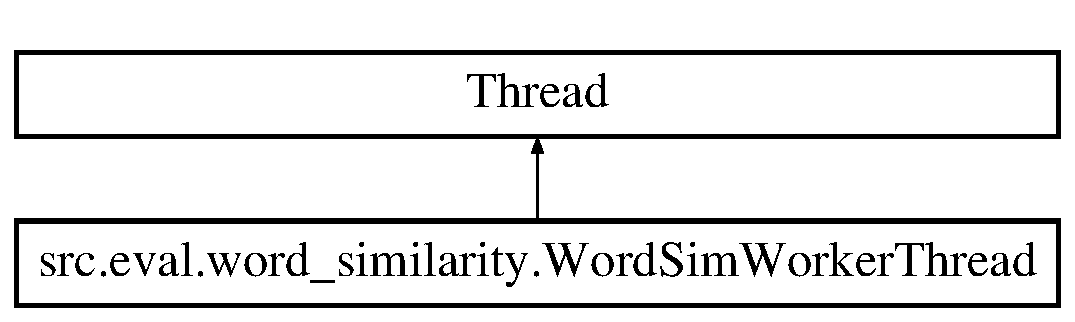
\includegraphics[height=2.000000cm]{classsrc_1_1eval_1_1word__similarity_1_1_word_sim_worker_thread}
\end{center}
\end{figure}
\subsection*{Public Member Functions}
\begin{DoxyCompactItemize}
\item 
def \hyperlink{classsrc_1_1eval_1_1word__similarity_1_1_word_sim_worker_thread_a3b3812382c5f42639526fb04e9cd669b}{\+\_\+\+\_\+init\+\_\+\+\_\+} (self, \hyperlink{classsrc_1_1eval_1_1word__similarity_1_1_word_sim_worker_thread_a37e8696ce9b04d6558d24f6f03852284}{worker\+\_\+id}, \hyperlink{classsrc_1_1eval_1_1word__similarity_1_1_word_sim_worker_thread_a22f86f1d8e6ba9b21656ae514bdcde05}{pair\+\_\+queue}, \hyperlink{classsrc_1_1eval_1_1word__similarity_1_1_word_sim_worker_thread_a71ee40a2cd50bb58d04300a80c27e73e}{model}, \hyperlink{classsrc_1_1eval_1_1word__similarity_1_1_word_sim_worker_thread_a0bd37d37430bab580530afb9c5769797}{y})
\item 
def \hyperlink{classsrc_1_1eval_1_1word__similarity_1_1_word_sim_worker_thread_a4d2dbdac00deb01c84b93fe4a65f6461}{run} (self)
\end{DoxyCompactItemize}
\subsection*{Public Attributes}
\begin{DoxyCompactItemize}
\item 
\hyperlink{classsrc_1_1eval_1_1word__similarity_1_1_word_sim_worker_thread_a37e8696ce9b04d6558d24f6f03852284}{worker\+\_\+id}
\item 
\hyperlink{classsrc_1_1eval_1_1word__similarity_1_1_word_sim_worker_thread_a22f86f1d8e6ba9b21656ae514bdcde05}{pair\+\_\+queue}
\item 
\hyperlink{classsrc_1_1eval_1_1word__similarity_1_1_word_sim_worker_thread_a71ee40a2cd50bb58d04300a80c27e73e}{model}
\item 
\hyperlink{classsrc_1_1eval_1_1word__similarity_1_1_word_sim_worker_thread_a0bd37d37430bab580530afb9c5769797}{y}
\item 
\hyperlink{classsrc_1_1eval_1_1word__similarity_1_1_word_sim_worker_thread_a7371b9cd48a94bb05db847e97d905038}{error\+\_\+count}
\end{DoxyCompactItemize}


\subsection{Constructor \& Destructor Documentation}
\index{src\+::eval\+::word\+\_\+similarity\+::\+Word\+Sim\+Worker\+Thread@{src\+::eval\+::word\+\_\+similarity\+::\+Word\+Sim\+Worker\+Thread}!\+\_\+\+\_\+init\+\_\+\+\_\+@{\+\_\+\+\_\+init\+\_\+\+\_\+}}
\index{\+\_\+\+\_\+init\+\_\+\+\_\+@{\+\_\+\+\_\+init\+\_\+\+\_\+}!src\+::eval\+::word\+\_\+similarity\+::\+Word\+Sim\+Worker\+Thread@{src\+::eval\+::word\+\_\+similarity\+::\+Word\+Sim\+Worker\+Thread}}
\subsubsection[{\texorpdfstring{\+\_\+\+\_\+init\+\_\+\+\_\+(self, worker\+\_\+id, pair\+\_\+queue, model, y)}{\_\_init\_\_(self, worker\_id, pair\_queue, model, y)}}]{\setlength{\rightskip}{0pt plus 5cm}def src.\+eval.\+word\+\_\+similarity.\+Word\+Sim\+Worker\+Thread.\+\_\+\+\_\+init\+\_\+\+\_\+ (
\begin{DoxyParamCaption}
\item[{}]{self, }
\item[{}]{worker\+\_\+id, }
\item[{}]{pair\+\_\+queue, }
\item[{}]{model, }
\item[{}]{y}
\end{DoxyParamCaption}
)}\hypertarget{classsrc_1_1eval_1_1word__similarity_1_1_word_sim_worker_thread_a3b3812382c5f42639526fb04e9cd669b}{}\label{classsrc_1_1eval_1_1word__similarity_1_1_word_sim_worker_thread_a3b3812382c5f42639526fb04e9cd669b}


\subsection{Member Function Documentation}
\index{src\+::eval\+::word\+\_\+similarity\+::\+Word\+Sim\+Worker\+Thread@{src\+::eval\+::word\+\_\+similarity\+::\+Word\+Sim\+Worker\+Thread}!run@{run}}
\index{run@{run}!src\+::eval\+::word\+\_\+similarity\+::\+Word\+Sim\+Worker\+Thread@{src\+::eval\+::word\+\_\+similarity\+::\+Word\+Sim\+Worker\+Thread}}
\subsubsection[{\texorpdfstring{run(self)}{run(self)}}]{\setlength{\rightskip}{0pt plus 5cm}def src.\+eval.\+word\+\_\+similarity.\+Word\+Sim\+Worker\+Thread.\+run (
\begin{DoxyParamCaption}
\item[{}]{self}
\end{DoxyParamCaption}
)}\hypertarget{classsrc_1_1eval_1_1word__similarity_1_1_word_sim_worker_thread_a4d2dbdac00deb01c84b93fe4a65f6461}{}\label{classsrc_1_1eval_1_1word__similarity_1_1_word_sim_worker_thread_a4d2dbdac00deb01c84b93fe4a65f6461}


\subsection{Member Data Documentation}
\index{src\+::eval\+::word\+\_\+similarity\+::\+Word\+Sim\+Worker\+Thread@{src\+::eval\+::word\+\_\+similarity\+::\+Word\+Sim\+Worker\+Thread}!error\+\_\+count@{error\+\_\+count}}
\index{error\+\_\+count@{error\+\_\+count}!src\+::eval\+::word\+\_\+similarity\+::\+Word\+Sim\+Worker\+Thread@{src\+::eval\+::word\+\_\+similarity\+::\+Word\+Sim\+Worker\+Thread}}
\subsubsection[{\texorpdfstring{error\+\_\+count}{error\_count}}]{\setlength{\rightskip}{0pt plus 5cm}src.\+eval.\+word\+\_\+similarity.\+Word\+Sim\+Worker\+Thread.\+error\+\_\+count}\hypertarget{classsrc_1_1eval_1_1word__similarity_1_1_word_sim_worker_thread_a7371b9cd48a94bb05db847e97d905038}{}\label{classsrc_1_1eval_1_1word__similarity_1_1_word_sim_worker_thread_a7371b9cd48a94bb05db847e97d905038}
\index{src\+::eval\+::word\+\_\+similarity\+::\+Word\+Sim\+Worker\+Thread@{src\+::eval\+::word\+\_\+similarity\+::\+Word\+Sim\+Worker\+Thread}!model@{model}}
\index{model@{model}!src\+::eval\+::word\+\_\+similarity\+::\+Word\+Sim\+Worker\+Thread@{src\+::eval\+::word\+\_\+similarity\+::\+Word\+Sim\+Worker\+Thread}}
\subsubsection[{\texorpdfstring{model}{model}}]{\setlength{\rightskip}{0pt plus 5cm}src.\+eval.\+word\+\_\+similarity.\+Word\+Sim\+Worker\+Thread.\+model}\hypertarget{classsrc_1_1eval_1_1word__similarity_1_1_word_sim_worker_thread_a71ee40a2cd50bb58d04300a80c27e73e}{}\label{classsrc_1_1eval_1_1word__similarity_1_1_word_sim_worker_thread_a71ee40a2cd50bb58d04300a80c27e73e}
\index{src\+::eval\+::word\+\_\+similarity\+::\+Word\+Sim\+Worker\+Thread@{src\+::eval\+::word\+\_\+similarity\+::\+Word\+Sim\+Worker\+Thread}!pair\+\_\+queue@{pair\+\_\+queue}}
\index{pair\+\_\+queue@{pair\+\_\+queue}!src\+::eval\+::word\+\_\+similarity\+::\+Word\+Sim\+Worker\+Thread@{src\+::eval\+::word\+\_\+similarity\+::\+Word\+Sim\+Worker\+Thread}}
\subsubsection[{\texorpdfstring{pair\+\_\+queue}{pair\_queue}}]{\setlength{\rightskip}{0pt plus 5cm}src.\+eval.\+word\+\_\+similarity.\+Word\+Sim\+Worker\+Thread.\+pair\+\_\+queue}\hypertarget{classsrc_1_1eval_1_1word__similarity_1_1_word_sim_worker_thread_a22f86f1d8e6ba9b21656ae514bdcde05}{}\label{classsrc_1_1eval_1_1word__similarity_1_1_word_sim_worker_thread_a22f86f1d8e6ba9b21656ae514bdcde05}
\index{src\+::eval\+::word\+\_\+similarity\+::\+Word\+Sim\+Worker\+Thread@{src\+::eval\+::word\+\_\+similarity\+::\+Word\+Sim\+Worker\+Thread}!worker\+\_\+id@{worker\+\_\+id}}
\index{worker\+\_\+id@{worker\+\_\+id}!src\+::eval\+::word\+\_\+similarity\+::\+Word\+Sim\+Worker\+Thread@{src\+::eval\+::word\+\_\+similarity\+::\+Word\+Sim\+Worker\+Thread}}
\subsubsection[{\texorpdfstring{worker\+\_\+id}{worker\_id}}]{\setlength{\rightskip}{0pt plus 5cm}src.\+eval.\+word\+\_\+similarity.\+Word\+Sim\+Worker\+Thread.\+worker\+\_\+id}\hypertarget{classsrc_1_1eval_1_1word__similarity_1_1_word_sim_worker_thread_a37e8696ce9b04d6558d24f6f03852284}{}\label{classsrc_1_1eval_1_1word__similarity_1_1_word_sim_worker_thread_a37e8696ce9b04d6558d24f6f03852284}
\index{src\+::eval\+::word\+\_\+similarity\+::\+Word\+Sim\+Worker\+Thread@{src\+::eval\+::word\+\_\+similarity\+::\+Word\+Sim\+Worker\+Thread}!y@{y}}
\index{y@{y}!src\+::eval\+::word\+\_\+similarity\+::\+Word\+Sim\+Worker\+Thread@{src\+::eval\+::word\+\_\+similarity\+::\+Word\+Sim\+Worker\+Thread}}
\subsubsection[{\texorpdfstring{y}{y}}]{\setlength{\rightskip}{0pt plus 5cm}src.\+eval.\+word\+\_\+similarity.\+Word\+Sim\+Worker\+Thread.\+y}\hypertarget{classsrc_1_1eval_1_1word__similarity_1_1_word_sim_worker_thread_a0bd37d37430bab580530afb9c5769797}{}\label{classsrc_1_1eval_1_1word__similarity_1_1_word_sim_worker_thread_a0bd37d37430bab580530afb9c5769797}


The documentation for this class was generated from the following file\+:\begin{DoxyCompactItemize}
\item 
/\+Users/dennisulmer/\+Documents/\+Studium/7. Semester/\+Computerlinguistik/\+Bachelorarbeit/src/eval/\hyperlink{word__similarity_8py}{word\+\_\+similarity.\+py}\end{DoxyCompactItemize}

\chapter{File Documentation}
\hypertarget{____init_____8py}{}\section{/\+Users/dennisulmer/\+Documents/\+Studium/7. Semester/\+Computerlinguistik/\+Bachelorarbeit/src/\+\_\+\+\_\+init\+\_\+\+\_\+.py File Reference}
\label{____init_____8py}\index{/\+Users/dennisulmer/\+Documents/\+Studium/7. Semester/\+Computerlinguistik/\+Bachelorarbeit/src/\+\_\+\+\_\+init\+\_\+\+\_\+.\+py@{/\+Users/dennisulmer/\+Documents/\+Studium/7. Semester/\+Computerlinguistik/\+Bachelorarbeit/src/\+\_\+\+\_\+init\+\_\+\+\_\+.\+py}}
\subsection*{Namespaces}
\begin{DoxyCompactItemize}
\item 
 \hyperlink{namespacesrc}{src}
\end{DoxyCompactItemize}

\hypertarget{clustering_2____init_____8py}{}\section{/\+Users/dennisulmer/\+Documents/\+Studium/7. Semester/\+Computerlinguistik/\+Bachelorarbeit/src/clustering/\+\_\+\+\_\+init\+\_\+\+\_\+.py File Reference}
\label{clustering_2____init_____8py}\index{/\+Users/dennisulmer/\+Documents/\+Studium/7. Semester/\+Computerlinguistik/\+Bachelorarbeit/src/clustering/\+\_\+\+\_\+init\+\_\+\+\_\+.\+py@{/\+Users/dennisulmer/\+Documents/\+Studium/7. Semester/\+Computerlinguistik/\+Bachelorarbeit/src/clustering/\+\_\+\+\_\+init\+\_\+\+\_\+.\+py}}
\subsection*{Namespaces}
\begin{DoxyCompactItemize}
\item 
 \hyperlink{namespacesrc_1_1clustering}{src.\+clustering}
\end{DoxyCompactItemize}

\hypertarget{eval_2____init_____8py}{}\section{/\+Users/dennisulmer/\+Documents/\+Studium/7. Semester/\+Computerlinguistik/\+Bachelorarbeit/src/eval/\+\_\+\+\_\+init\+\_\+\+\_\+.py File Reference}
\label{eval_2____init_____8py}\index{/\+Users/dennisulmer/\+Documents/\+Studium/7. Semester/\+Computerlinguistik/\+Bachelorarbeit/src/eval/\+\_\+\+\_\+init\+\_\+\+\_\+.\+py@{/\+Users/dennisulmer/\+Documents/\+Studium/7. Semester/\+Computerlinguistik/\+Bachelorarbeit/src/eval/\+\_\+\+\_\+init\+\_\+\+\_\+.\+py}}
\subsection*{Namespaces}
\begin{DoxyCompactItemize}
\item 
 \hyperlink{namespacesrc_1_1eval}{src.\+eval}
\end{DoxyCompactItemize}

\hypertarget{guesser_2____init_____8py}{}\section{/\+Users/dennisulmer/\+Documents/\+Studium/7. Semester/\+Computerlinguistik/\+Bachelorarbeit/src/guesser/\+\_\+\+\_\+init\+\_\+\+\_\+.py File Reference}
\label{guesser_2____init_____8py}\index{/\+Users/dennisulmer/\+Documents/\+Studium/7. Semester/\+Computerlinguistik/\+Bachelorarbeit/src/guesser/\+\_\+\+\_\+init\+\_\+\+\_\+.\+py@{/\+Users/dennisulmer/\+Documents/\+Studium/7. Semester/\+Computerlinguistik/\+Bachelorarbeit/src/guesser/\+\_\+\+\_\+init\+\_\+\+\_\+.\+py}}
\subsection*{Namespaces}
\begin{DoxyCompactItemize}
\item 
 \hyperlink{namespacesrc_1_1guesser}{src.\+guesser}
\end{DoxyCompactItemize}

\hypertarget{mapping_2____init_____8py}{}\section{/\+Users/dennisulmer/\+Documents/\+Studium/7. Semester/\+Computerlinguistik/\+Bachelorarbeit/src/mapping/\+\_\+\+\_\+init\+\_\+\+\_\+.py File Reference}
\label{mapping_2____init_____8py}\index{/\+Users/dennisulmer/\+Documents/\+Studium/7. Semester/\+Computerlinguistik/\+Bachelorarbeit/src/mapping/\+\_\+\+\_\+init\+\_\+\+\_\+.\+py@{/\+Users/dennisulmer/\+Documents/\+Studium/7. Semester/\+Computerlinguistik/\+Bachelorarbeit/src/mapping/\+\_\+\+\_\+init\+\_\+\+\_\+.\+py}}
\subsection*{Namespaces}
\begin{DoxyCompactItemize}
\item 
 \hyperlink{namespacesrc_1_1mapping}{src.\+mapping}
\end{DoxyCompactItemize}

\hypertarget{prep_2____init_____8py}{}\section{/\+Users/dennisulmer/\+Documents/\+Studium/7. Semester/\+Computerlinguistik/\+Bachelorarbeit/src/prep/\+\_\+\+\_\+init\+\_\+\+\_\+.py File Reference}
\label{prep_2____init_____8py}\index{/\+Users/dennisulmer/\+Documents/\+Studium/7. Semester/\+Computerlinguistik/\+Bachelorarbeit/src/prep/\+\_\+\+\_\+init\+\_\+\+\_\+.\+py@{/\+Users/dennisulmer/\+Documents/\+Studium/7. Semester/\+Computerlinguistik/\+Bachelorarbeit/src/prep/\+\_\+\+\_\+init\+\_\+\+\_\+.\+py}}
\subsection*{Namespaces}
\begin{DoxyCompactItemize}
\item 
 \hyperlink{namespacesrc_1_1prep}{src.\+prep}
\end{DoxyCompactItemize}

\hypertarget{prep_2corpus_2____init_____8py}{}\section{/\+Users/dennisulmer/\+Documents/\+Studium/7. Semester/\+Computerlinguistik/\+Bachelorarbeit/src/prep/corpus/\+\_\+\+\_\+init\+\_\+\+\_\+.py File Reference}
\label{prep_2corpus_2____init_____8py}\index{/\+Users/dennisulmer/\+Documents/\+Studium/7. Semester/\+Computerlinguistik/\+Bachelorarbeit/src/prep/corpus/\+\_\+\+\_\+init\+\_\+\+\_\+.\+py@{/\+Users/dennisulmer/\+Documents/\+Studium/7. Semester/\+Computerlinguistik/\+Bachelorarbeit/src/prep/corpus/\+\_\+\+\_\+init\+\_\+\+\_\+.\+py}}
\subsection*{Namespaces}
\begin{DoxyCompactItemize}
\item 
 \hyperlink{namespacesrc_1_1prep_1_1corpus}{src.\+prep.\+corpus}
\end{DoxyCompactItemize}

\hypertarget{prep_2dependencies_2____init_____8py}{}\section{/\+Users/dennisulmer/\+Documents/\+Studium/7. Semester/\+Computerlinguistik/\+Bachelorarbeit/src/prep/dependencies/\+\_\+\+\_\+init\+\_\+\+\_\+.py File Reference}
\label{prep_2dependencies_2____init_____8py}\index{/\+Users/dennisulmer/\+Documents/\+Studium/7. Semester/\+Computerlinguistik/\+Bachelorarbeit/src/prep/dependencies/\+\_\+\+\_\+init\+\_\+\+\_\+.\+py@{/\+Users/dennisulmer/\+Documents/\+Studium/7. Semester/\+Computerlinguistik/\+Bachelorarbeit/src/prep/dependencies/\+\_\+\+\_\+init\+\_\+\+\_\+.\+py}}
\subsection*{Namespaces}
\begin{DoxyCompactItemize}
\item 
 \hyperlink{namespacesrc_1_1prep_1_1dependencies}{src.\+prep.\+dependencies}
\end{DoxyCompactItemize}

\hypertarget{prep_2misc_2____init_____8py}{}\section{/\+Users/dennisulmer/\+Documents/\+Studium/7. Semester/\+Computerlinguistik/\+Bachelorarbeit/src/prep/misc/\+\_\+\+\_\+init\+\_\+\+\_\+.py File Reference}
\label{prep_2misc_2____init_____8py}\index{/\+Users/dennisulmer/\+Documents/\+Studium/7. Semester/\+Computerlinguistik/\+Bachelorarbeit/src/prep/misc/\+\_\+\+\_\+init\+\_\+\+\_\+.\+py@{/\+Users/dennisulmer/\+Documents/\+Studium/7. Semester/\+Computerlinguistik/\+Bachelorarbeit/src/prep/misc/\+\_\+\+\_\+init\+\_\+\+\_\+.\+py}}
\subsection*{Namespaces}
\begin{DoxyCompactItemize}
\item 
 \hyperlink{namespacesrc_1_1prep_1_1misc}{src.\+prep.\+misc}
\end{DoxyCompactItemize}

\hypertarget{prep_2nes_2____init_____8py}{}\section{/\+Users/dennisulmer/\+Documents/\+Studium/7. Semester/\+Computerlinguistik/\+Bachelorarbeit/src/prep/nes/\+\_\+\+\_\+init\+\_\+\+\_\+.py File Reference}
\label{prep_2nes_2____init_____8py}\index{/\+Users/dennisulmer/\+Documents/\+Studium/7. Semester/\+Computerlinguistik/\+Bachelorarbeit/src/prep/nes/\+\_\+\+\_\+init\+\_\+\+\_\+.\+py@{/\+Users/dennisulmer/\+Documents/\+Studium/7. Semester/\+Computerlinguistik/\+Bachelorarbeit/src/prep/nes/\+\_\+\+\_\+init\+\_\+\+\_\+.\+py}}
\subsection*{Namespaces}
\begin{DoxyCompactItemize}
\item 
 \hyperlink{namespacesrc_1_1prep_1_1nes}{src.\+prep.\+nes}
\end{DoxyCompactItemize}

\hypertarget{prep_2relations_2____init_____8py}{}\section{/\+Users/dennisulmer/\+Documents/\+Studium/7. Semester/\+Computerlinguistik/\+Bachelorarbeit/src/prep/relations/\+\_\+\+\_\+init\+\_\+\+\_\+.py File Reference}
\label{prep_2relations_2____init_____8py}\index{/\+Users/dennisulmer/\+Documents/\+Studium/7. Semester/\+Computerlinguistik/\+Bachelorarbeit/src/prep/relations/\+\_\+\+\_\+init\+\_\+\+\_\+.\+py@{/\+Users/dennisulmer/\+Documents/\+Studium/7. Semester/\+Computerlinguistik/\+Bachelorarbeit/src/prep/relations/\+\_\+\+\_\+init\+\_\+\+\_\+.\+py}}
\subsection*{Namespaces}
\begin{DoxyCompactItemize}
\item 
 \hyperlink{namespacesrc_1_1prep_1_1relations}{src.\+prep.\+relations}
\end{DoxyCompactItemize}

\hypertarget{trans__e_2____init_____8py}{}\section{/\+Users/dennisulmer/\+Documents/\+Studium/7. Semester/\+Computerlinguistik/\+Bachelorarbeit/src/trans\+\_\+e/\+\_\+\+\_\+init\+\_\+\+\_\+.py File Reference}
\label{trans__e_2____init_____8py}\index{/\+Users/dennisulmer/\+Documents/\+Studium/7. Semester/\+Computerlinguistik/\+Bachelorarbeit/src/trans\+\_\+e/\+\_\+\+\_\+init\+\_\+\+\_\+.\+py@{/\+Users/dennisulmer/\+Documents/\+Studium/7. Semester/\+Computerlinguistik/\+Bachelorarbeit/src/trans\+\_\+e/\+\_\+\+\_\+init\+\_\+\+\_\+.\+py}}
\subsection*{Namespaces}
\begin{DoxyCompactItemize}
\item 
 \hyperlink{namespacesrc_1_1trans__e}{src.\+trans\+\_\+e}
\end{DoxyCompactItemize}

\hypertarget{cluster__mappings_8py}{}\section{/\+Users/dennisulmer/\+Documents/\+Studium/7. Semester/\+Computerlinguistik/\+Bachelorarbeit/src/clustering/cluster\+\_\+mappings.py File Reference}
\label{cluster__mappings_8py}\index{/\+Users/dennisulmer/\+Documents/\+Studium/7. Semester/\+Computerlinguistik/\+Bachelorarbeit/src/clustering/cluster\+\_\+mappings.\+py@{/\+Users/dennisulmer/\+Documents/\+Studium/7. Semester/\+Computerlinguistik/\+Bachelorarbeit/src/clustering/cluster\+\_\+mappings.\+py}}
\subsection*{Namespaces}
\begin{DoxyCompactItemize}
\item 
 \hyperlink{namespacesrc_1_1clustering_1_1cluster__mappings}{src.\+clustering.\+cluster\+\_\+mappings}
\end{DoxyCompactItemize}
\subsection*{Functions}
\begin{DoxyCompactItemize}
\item 
def \hyperlink{namespacesrc_1_1clustering_1_1cluster__mappings_a88fac149a2f50ab788d49641e40eff26}{src.\+clustering.\+cluster\+\_\+mappings.\+main} ()
\item 
def \hyperlink{namespacesrc_1_1clustering_1_1cluster__mappings_abe09f35ebed7355349cb8e4d4449d352}{src.\+clustering.\+cluster\+\_\+mappings.\+train\+\_\+clustering\+\_\+parameters} (vector\+\_\+inpath)
\item 
def \hyperlink{namespacesrc_1_1clustering_1_1cluster__mappings_a20f212f41bf9a610ec0b8582054f0eae}{src.\+clustering.\+cluster\+\_\+mappings.\+cluster\+\_\+mappings} (vector\+\_\+inpath, do\+\_\+pca=False, target\+\_\+dim=100, indices\+\_\+inpath=None, epsilon=2.\+5, min\+\_\+s=20)
\item 
def \hyperlink{namespacesrc_1_1clustering_1_1cluster__mappings_aea338d4bf7a937a56ef575d1675c28d7}{src.\+clustering.\+cluster\+\_\+mappings.\+resolve\+\_\+indices} (points, labels, indices\+\_\+inpath, model)
\item 
def \hyperlink{namespacesrc_1_1clustering_1_1cluster__mappings_accdc0539121b7bd8d2368cccbfeef4a3}{src.\+clustering.\+cluster\+\_\+mappings.\+aggregate\+\_\+cluster} (points, labels)
\item 
def \hyperlink{namespacesrc_1_1clustering_1_1cluster__mappings_a58faafde39604ae8247b4946f8292541}{src.\+clustering.\+cluster\+\_\+mappings.\+load\+\_\+indices} (indices\+\_\+inpath)
\item 
def \hyperlink{namespacesrc_1_1clustering_1_1cluster__mappings_afc033e44dfb5c6953c53314f6f86e22e}{src.\+clustering.\+cluster\+\_\+mappings.\+get\+\_\+cluster\+\_\+size} (labels)
\item 
def \hyperlink{namespacesrc_1_1clustering_1_1cluster__mappings_a59e6668560bdac9085a9d6ab364a9d0d}{src.\+clustering.\+cluster\+\_\+mappings.\+load\+\_\+mappings\+\_\+from\+\_\+model} (mapping\+\_\+inpath)
\item 
def \hyperlink{namespacesrc_1_1clustering_1_1cluster__mappings_a69ce1b3be3ed909458b8f9dfe90d7585}{src.\+clustering.\+cluster\+\_\+mappings.\+alt} (func)
\item 
def \hyperlink{namespacesrc_1_1clustering_1_1cluster__mappings_ae22fbf49e267ac9c9640c33c0ee4f1f1}{src.\+clustering.\+cluster\+\_\+mappings.\+init\+\_\+argparser} ()
\end{DoxyCompactItemize}

\hypertarget{analogy_8py}{}\section{/\+Users/dennisulmer/\+Documents/\+Studium/7. Semester/\+Computerlinguistik/\+Bachelorarbeit/src/eval/analogy.py File Reference}
\label{analogy_8py}\index{/\+Users/dennisulmer/\+Documents/\+Studium/7. Semester/\+Computerlinguistik/\+Bachelorarbeit/src/eval/analogy.\+py@{/\+Users/dennisulmer/\+Documents/\+Studium/7. Semester/\+Computerlinguistik/\+Bachelorarbeit/src/eval/analogy.\+py}}
\subsection*{Classes}
\begin{DoxyCompactItemize}
\item 
class \hyperlink{classsrc_1_1eval_1_1analogy_1_1_analogy_master_thread}{src.\+eval.\+analogy.\+Analogy\+Master\+Thread}
\item 
class \hyperlink{classsrc_1_1eval_1_1analogy_1_1_analogy_worker_thread}{src.\+eval.\+analogy.\+Analogy\+Worker\+Thread}
\end{DoxyCompactItemize}
\subsection*{Namespaces}
\begin{DoxyCompactItemize}
\item 
 \hyperlink{namespacesrc_1_1eval_1_1analogy}{src.\+eval.\+analogy}
\end{DoxyCompactItemize}
\subsection*{Functions}
\begin{DoxyCompactItemize}
\item 
def \hyperlink{namespacesrc_1_1eval_1_1analogy_ab329d7279b400a1d3a8774dc86c94c8f}{src.\+eval.\+analogy.\+analogy\+\_\+eval\+\_\+parallel} (vector\+\_\+inpath, analogy\+\_\+path, per\+\_\+section=False, logpath=None, threads=1)
\item 
def \hyperlink{namespacesrc_1_1eval_1_1analogy_a50e9e7514b6687e8fdde2700363fc4d7}{src.\+eval.\+analogy.\+analogy\+\_\+eval} (vector\+\_\+inpath, analogy\+\_\+path, per\+\_\+section=False, logpath=None)
\item 
def \hyperlink{namespacesrc_1_1eval_1_1analogy_ade7b9f54c3edfb9a2d418c0b39d63e2f}{src.\+eval.\+analogy.\+read\+\_\+analogies} (analogy\+\_\+path, per\+\_\+section=False)
\item 
def \hyperlink{namespacesrc_1_1eval_1_1analogy_a90785f17ab2d275fc18216914fe79e60}{src.\+eval.\+analogy.\+read\+\_\+analogies\+\_\+for\+\_\+parallel} (analogy\+\_\+path, per\+\_\+section=False)
\item 
def \hyperlink{namespacesrc_1_1eval_1_1analogy_ae7d3794d8d951a6dd9652f163af5a19c}{src.\+eval.\+analogy.\+output} (message, logpath=None)
\item 
def \hyperlink{namespacesrc_1_1eval_1_1analogy_aaeab378b9b3988b8fa1c101c227a99d9}{src.\+eval.\+analogy.\+rreplace} (s, old, new, occurrence)
\end{DoxyCompactItemize}

\hypertarget{concentration_8py}{}\section{/\+Users/dennisulmer/\+Documents/\+Studium/7. Semester/\+Computerlinguistik/\+Bachelorarbeit/src/eval/concentration.py File Reference}
\label{concentration_8py}\index{/\+Users/dennisulmer/\+Documents/\+Studium/7. Semester/\+Computerlinguistik/\+Bachelorarbeit/src/eval/concentration.\+py@{/\+Users/dennisulmer/\+Documents/\+Studium/7. Semester/\+Computerlinguistik/\+Bachelorarbeit/src/eval/concentration.\+py}}
\subsection*{Namespaces}
\begin{DoxyCompactItemize}
\item 
 \hyperlink{namespacesrc_1_1eval_1_1concentration}{src.\+eval.\+concentration}
\end{DoxyCompactItemize}
\subsection*{Functions}
\begin{DoxyCompactItemize}
\item 
def \hyperlink{namespacesrc_1_1eval_1_1concentration_a39d2edb93fad1c1766b1107c9954c1f3}{src.\+eval.\+concentration.\+calculate\+\_\+loss\+\_\+of\+\_\+precision} (vector\+\_\+inpath, procs, sizes, logpath=None)
\item 
def \hyperlink{namespacesrc_1_1eval_1_1concentration_a2f99b5b9b58322935a7ca7bb766cbbb9}{src.\+eval.\+concentration.\+calculate\+\_\+concentrations} (vectors\+\_\+inpath, procs, max\+\_\+n\+\_\+vectors, logpath=None)
\item 
def \hyperlink{namespacesrc_1_1eval_1_1concentration_a33987fe9eae3decb05601e868dfad18d}{src.\+eval.\+concentration.\+calculate\+\_\+concentration} (model, procs, logpath=None, vector\+\_\+inpath=\char`\"{}\char`\"{})
\item 
def \hyperlink{namespacesrc_1_1eval_1_1concentration_ab24bba4b57c8a848405d5d9c31b31525}{src.\+eval.\+concentration.\+\_\+calculate\+\_\+all\+\_\+distances} (cargs)
\item 
def \hyperlink{namespacesrc_1_1eval_1_1concentration_ac5dd136b31204c794d232af89857bd7a}{src.\+eval.\+concentration.\+\_\+calculate\+\_\+deviance} (dargs)
\item 
def \hyperlink{namespacesrc_1_1eval_1_1concentration_a235768292b5e81872b7caba8f9f37e64}{src.\+eval.\+concentration.\+chunks} (l, n)
\item 
def \hyperlink{namespacesrc_1_1eval_1_1concentration_a55c484721d01a583be952ac6206e659b}{src.\+eval.\+concentration.\+chunks2} (lst, n)
\item 
def \hyperlink{namespacesrc_1_1eval_1_1concentration_a1ea43a2b9635093100411e9e2ec40bb0}{src.\+eval.\+concentration.\+init\+\_\+pool\+\_\+for\+\_\+distances} (pool\+\_\+args)
\item 
def \hyperlink{namespacesrc_1_1eval_1_1concentration_a916888eea5c2c3033aa8fcbcba31c200}{src.\+eval.\+concentration.\+init\+\_\+pool\+\_\+for\+\_\+deviances} (pool\+\_\+args)
\item 
def \hyperlink{namespacesrc_1_1eval_1_1concentration_aef7e62814401c5b3f733b09223cbea37}{src.\+eval.\+concentration.\+output} (message, logpath=None)
\item 
def \hyperlink{namespacesrc_1_1eval_1_1concentration_a10f9e4ef2f6118f682345ef3d1cdb013}{src.\+eval.\+concentration.\+alt} (func)
\item 
def \hyperlink{namespacesrc_1_1eval_1_1concentration_a499c9e8d16fea63bc32addf0cb2eabcc}{src.\+eval.\+concentration.\+load\+\_\+vectors\+\_\+from\+\_\+model} (vector\+\_\+inpath, max\+\_\+n=None, logpath=None, indices=False)
\item 
def \hyperlink{namespacesrc_1_1eval_1_1concentration_a6010f2ae026a691e03eae46b46c04f84}{src.\+eval.\+concentration.\+load\+\_\+vectors\+\_\+from\+\_\+model\+\_\+parallel} (vector\+\_\+inpath, procs, logpath=None)
\item 
def \hyperlink{namespacesrc_1_1eval_1_1concentration_a98ece19ecbb403b8aa83fccf577152fe}{src.\+eval.\+concentration.\+rreplace} (s, old, new, occurrence)
\end{DoxyCompactItemize}
\subsection*{Variables}
\begin{DoxyCompactItemize}
\item 
\hyperlink{namespacesrc_1_1eval_1_1concentration_a31fc2d0b98a6e58bf5930064d0ce250c}{src.\+eval.\+concentration.\+n}
\end{DoxyCompactItemize}

\hypertarget{concept__groups_8py}{}\section{/\+Users/dennisulmer/\+Documents/\+Studium/7. Semester/\+Computerlinguistik/\+Bachelorarbeit/src/eval/concept\+\_\+groups.py File Reference}
\label{concept__groups_8py}\index{/\+Users/dennisulmer/\+Documents/\+Studium/7. Semester/\+Computerlinguistik/\+Bachelorarbeit/src/eval/concept\+\_\+groups.\+py@{/\+Users/dennisulmer/\+Documents/\+Studium/7. Semester/\+Computerlinguistik/\+Bachelorarbeit/src/eval/concept\+\_\+groups.\+py}}
\subsection*{Namespaces}
\begin{DoxyCompactItemize}
\item 
 \hyperlink{namespacesrc_1_1eval_1_1concept__groups}{src.\+eval.\+concept\+\_\+groups}
\end{DoxyCompactItemize}
\subsection*{Functions}
\begin{DoxyCompactItemize}
\item 
def \hyperlink{namespacesrc_1_1eval_1_1concept__groups_a2c78e489c17fc8cf3f0e81cfd6268d9d}{src.\+eval.\+concept\+\_\+groups.\+main} ()
\item 
def \hyperlink{namespacesrc_1_1eval_1_1concept__groups_a51c1c326e30e374319dd90a08a91a979}{src.\+eval.\+concept\+\_\+groups.\+sample\+Relations} (inpath, outpath, n, sample\+\_\+size, freq\+\_\+constraint)
\item 
def \hyperlink{namespacesrc_1_1eval_1_1concept__groups_a4bf6c7ef4b109f0bb3a4241aa36b6ad3}{src.\+eval.\+concept\+\_\+groups.\+sample\+\_\+part} (relation\+\_\+pairs, coin\+\_\+flip, sample\+\_\+size)
\item 
def \hyperlink{namespacesrc_1_1eval_1_1concept__groups_a8930fd427aabc8e9e3f1c0fd3357171a}{src.\+eval.\+concept\+\_\+groups.\+take\+\_\+sample\+\_\+from\+\_\+list} (samplelist, n)
\end{DoxyCompactItemize}

\hypertarget{eval__vectors_8py}{}\section{/\+Users/dennisulmer/\+Documents/\+Studium/7. Semester/\+Computerlinguistik/\+Bachelorarbeit/src/eval/eval\+\_\+vectors.py File Reference}
\label{eval__vectors_8py}\index{/\+Users/dennisulmer/\+Documents/\+Studium/7. Semester/\+Computerlinguistik/\+Bachelorarbeit/src/eval/eval\+\_\+vectors.\+py@{/\+Users/dennisulmer/\+Documents/\+Studium/7. Semester/\+Computerlinguistik/\+Bachelorarbeit/src/eval/eval\+\_\+vectors.\+py}}
\subsection*{Namespaces}
\begin{DoxyCompactItemize}
\item 
 \hyperlink{namespacesrc_1_1eval_1_1eval__vectors}{src.\+eval.\+eval\+\_\+vectors}
\end{DoxyCompactItemize}
\subsection*{Functions}
\begin{DoxyCompactItemize}
\item 
def \hyperlink{namespacesrc_1_1eval_1_1eval__vectors_a3ccd3f48a0989935dc27045a598737df}{src.\+eval.\+eval\+\_\+vectors.\+main} ()
\item 
def \hyperlink{namespacesrc_1_1eval_1_1eval__vectors_a3cf87b490f0d115602b0511b02960c5a}{src.\+eval.\+eval\+\_\+vectors.\+find\+\_\+nearest\+\_\+neighbors} (vector\+\_\+inpath, max, wordlist)
\item 
def \hyperlink{namespacesrc_1_1eval_1_1eval__vectors_a6168d2cb3dff1d01ff10ed4127850dec}{src.\+eval.\+eval\+\_\+vectors.\+plot} (data, max, dimensions, show\+\_\+plot=False, display\+\_\+names=False)
\item 
def \hyperlink{namespacesrc_1_1eval_1_1eval__vectors_a279f181f952a4d6365293688afbb5355}{src.\+eval.\+eval\+\_\+vectors.\+plot\+\_\+distance\+\_\+distribution} (data, max, show\+\_\+plot=False)
\item 
def \hyperlink{namespacesrc_1_1eval_1_1eval__vectors_ad6d96a02ca305eccf4e2f45dae69ad58}{src.\+eval.\+eval\+\_\+vectors.\+opt\+\_\+callback} (option, opt, value, parser)
\item 
def \hyperlink{namespacesrc_1_1eval_1_1eval__vectors_aeec8ba68a1e7aef91b52c1ca32642ab8}{src.\+eval.\+eval\+\_\+vectors.\+apply\+\_\+on\+\_\+input} (func, sets, inpath, args)
\item 
def \hyperlink{namespacesrc_1_1eval_1_1eval__vectors_acbe16d31d9d730b59c114a528f4fb64d}{src.\+eval.\+eval\+\_\+vectors.\+output} (message, logpath=None)
\item 
def \hyperlink{namespacesrc_1_1eval_1_1eval__vectors_abed4618328dd07d5e688310742b194ae}{src.\+eval.\+eval\+\_\+vectors.\+rreplace} (s, old, new, occurrence)
\item 
def \hyperlink{namespacesrc_1_1eval_1_1eval__vectors_afc3aa8c78c129a423c6d8cc134d7d1f8}{src.\+eval.\+eval\+\_\+vectors.\+init\+\_\+argparser} ()
\end{DoxyCompactItemize}

\hypertarget{word__similarity_8py}{}\section{/\+Users/dennisulmer/\+Documents/\+Studium/7. Semester/\+Computerlinguistik/\+Bachelorarbeit/src/eval/word\+\_\+similarity.py File Reference}
\label{word__similarity_8py}\index{/\+Users/dennisulmer/\+Documents/\+Studium/7. Semester/\+Computerlinguistik/\+Bachelorarbeit/src/eval/word\+\_\+similarity.\+py@{/\+Users/dennisulmer/\+Documents/\+Studium/7. Semester/\+Computerlinguistik/\+Bachelorarbeit/src/eval/word\+\_\+similarity.\+py}}
\subsection*{Classes}
\begin{DoxyCompactItemize}
\item 
class \hyperlink{classsrc_1_1eval_1_1word__similarity_1_1_word_sim_master_thread}{src.\+eval.\+word\+\_\+similarity.\+Word\+Sim\+Master\+Thread}
\item 
class \hyperlink{classsrc_1_1eval_1_1word__similarity_1_1_word_sim_worker_thread}{src.\+eval.\+word\+\_\+similarity.\+Word\+Sim\+Worker\+Thread}
\end{DoxyCompactItemize}
\subsection*{Namespaces}
\begin{DoxyCompactItemize}
\item 
 \hyperlink{namespacesrc_1_1eval_1_1word__similarity}{src.\+eval.\+word\+\_\+similarity}
\end{DoxyCompactItemize}
\subsection*{Functions}
\begin{DoxyCompactItemize}
\item 
def \hyperlink{namespacesrc_1_1eval_1_1word__similarity_a1354f52478e8c8a08ab45fd57bc98900}{src.\+eval.\+word\+\_\+similarity.\+parallel\+\_\+word\+\_\+sim\+\_\+eval} (vector\+\_\+inpath, wordpair\+\_\+path, logpath, format=\char`\"{}google\char`\"{}, threads=1)
\item 
def \hyperlink{namespacesrc_1_1eval_1_1word__similarity_a625968df4faf09a29c29114eccfd1a25}{src.\+eval.\+word\+\_\+similarity.\+word\+\_\+sim\+\_\+eval} (vector\+\_\+inpath, wordpair\+\_\+path, logpath, format=\char`\"{}google\char`\"{})
\item 
def \hyperlink{namespacesrc_1_1eval_1_1word__similarity_a35413ae9492d04d2287dc9ef6b4a65fe}{src.\+eval.\+word\+\_\+similarity.\+remove\+\_\+unknowns} (x, y)
\item 
def \hyperlink{namespacesrc_1_1eval_1_1word__similarity_abea02377530269660e7b87bb6b587e90}{src.\+eval.\+word\+\_\+similarity.\+capitalize} (word)
\item 
def \hyperlink{namespacesrc_1_1eval_1_1word__similarity_a39c65ceec0a33401a8e87f56a8d1d71b}{src.\+eval.\+word\+\_\+similarity.\+evaluate\+\_\+wordpair\+\_\+sims} (x, y, number\+\_\+of\+\_\+pairs)
\item 
def \hyperlink{namespacesrc_1_1eval_1_1word__similarity_ae8cf8c4fbd45bc31c5487c5287343973}{src.\+eval.\+word\+\_\+similarity.\+read\+\_\+wordpairs} (wordpair\+\_\+path, format=\char`\"{}google\char`\"{})
\item 
def \hyperlink{namespacesrc_1_1eval_1_1word__similarity_a297370f72df98c0c9596594cfa741f70}{src.\+eval.\+word\+\_\+similarity.\+output} (message, logpath=None)
\item 
def \hyperlink{namespacesrc_1_1eval_1_1word__similarity_ab07a8c8006268073ec010c38d74b307e}{src.\+eval.\+word\+\_\+similarity.\+rreplace} (s, old, new, occurrence)
\end{DoxyCompactItemize}

\hypertarget{svm__guesser_8py}{}\section{/\+Users/dennisulmer/\+Documents/\+Studium/7. Semester/\+Computerlinguistik/\+Bachelorarbeit/src/guesser/svm\+\_\+guesser.py File Reference}
\label{svm__guesser_8py}\index{/\+Users/dennisulmer/\+Documents/\+Studium/7. Semester/\+Computerlinguistik/\+Bachelorarbeit/src/guesser/svm\+\_\+guesser.\+py@{/\+Users/dennisulmer/\+Documents/\+Studium/7. Semester/\+Computerlinguistik/\+Bachelorarbeit/src/guesser/svm\+\_\+guesser.\+py}}
\subsection*{Namespaces}
\begin{DoxyCompactItemize}
\item 
 \hyperlink{namespacesrc_1_1guesser_1_1svm__guesser}{src.\+guesser.\+svm\+\_\+guesser}
\end{DoxyCompactItemize}
\subsection*{Functions}
\begin{DoxyCompactItemize}
\item 
def \hyperlink{namespacesrc_1_1guesser_1_1svm__guesser_af0a15ec0f6bea29bc99fcce23bd3ebb0}{src.\+guesser.\+svm\+\_\+guesser.\+main} ()
\item 
def \hyperlink{namespacesrc_1_1guesser_1_1svm__guesser_a8c54c05a7a892e16fc90f7453498a04d}{src.\+guesser.\+svm\+\_\+guesser.\+prepare\+\_\+training} (sets\+\_\+path, vector\+\_\+inpath)
\item 
def \hyperlink{namespacesrc_1_1guesser_1_1svm__guesser_a864007265fbd9dcc2dbc2437499ff3f6}{src.\+guesser.\+svm\+\_\+guesser.\+train} (model, grouped\+\_\+train, grouped\+\_\+corrupted, lossf, relation\+\_\+types, epochs=1000, learning\+\_\+rate=0.\+01, margin=1)
\item 
def \hyperlink{namespacesrc_1_1guesser_1_1svm__guesser_ad86de62133a12499bf18fa8910bba858}{src.\+guesser.\+svm\+\_\+guesser.\+\_\+stupid\+\_\+train} (model, grouped\+\_\+train, relation\+\_\+types)
\item 
def \hyperlink{namespacesrc_1_1guesser_1_1svm__guesser_ad415894d44f4d9a422c31fb45f34ec89}{src.\+guesser.\+svm\+\_\+guesser.\+evaluate} (model, grouped\+\_\+test, relation\+\_\+vectors, entities)
\item 
def \hyperlink{namespacesrc_1_1guesser_1_1svm__guesser_a9b3dc374f8fe43fa22ab034de3c01cf4}{src.\+guesser.\+svm\+\_\+guesser.\+rank\+\_\+entities} (reference, solution, model, entities)
\item 
def \hyperlink{namespacesrc_1_1guesser_1_1svm__guesser_a5bdc93643767e3cb2eb120cf09983702}{src.\+guesser.\+svm\+\_\+guesser.\+get\+\_\+rank} (target, ranks)
\item 
def \hyperlink{namespacesrc_1_1guesser_1_1svm__guesser_a46c3bf2fd1c519e3014007828c33c64d}{src.\+guesser.\+svm\+\_\+guesser.\+create\+\_\+corrupt\+\_\+triples} (grouped\+\_\+pairs, entities)
\item 
def \hyperlink{namespacesrc_1_1guesser_1_1svm__guesser_a90e7986eb6b2f54ff825144cc31d5072}{src.\+guesser.\+svm\+\_\+guesser.\+transform\+\_\+triples} (triples, relation\+\_\+types, entities)
\item 
def \hyperlink{namespacesrc_1_1guesser_1_1svm__guesser_ab129201b9264ddfb4e334b40366aa4e6}{src.\+guesser.\+svm\+\_\+guesser.\+convert\+\_\+data} (sets\+\_\+path, tql\+\_\+inpath, vector\+\_\+inpath)
\item 
def \hyperlink{namespacesrc_1_1guesser_1_1svm__guesser_a60328a23b11cb5ea2fc6deef915b6b89}{src.\+guesser.\+svm\+\_\+guesser.\+write\+\_\+data} (triples, found\+\_\+entities, outpath)
\item 
def \hyperlink{namespacesrc_1_1guesser_1_1svm__guesser_a57c8a51581590ac0df4a7d07a27893a6}{src.\+guesser.\+svm\+\_\+guesser.\+read\+\_\+freebase\+\_\+data} (sets\+\_\+path)
\item 
def \hyperlink{namespacesrc_1_1guesser_1_1svm__guesser_aeb0faa67c606038dc3936ee21db34b03}{src.\+guesser.\+svm\+\_\+guesser.\+read\+\_\+freebase\+\_\+file} (fb\+\_\+inpath)
\item 
def \hyperlink{namespacesrc_1_1guesser_1_1svm__guesser_a07427a8ed0aa8653f8b8faa8fa6f65b5}{src.\+guesser.\+svm\+\_\+guesser.\+read\+\_\+tql\+\_\+file} (tql\+\_\+inpath)
\item 
def \hyperlink{namespacesrc_1_1guesser_1_1svm__guesser_ab43ef3856a80d03d726fc97c7eba5a5a}{src.\+guesser.\+svm\+\_\+guesser.\+dump\+\_\+relation\+\_\+vectors} (relation\+\_\+vectors, outpath)
\item 
def \hyperlink{namespacesrc_1_1guesser_1_1svm__guesser_aa586eda223e1a50888189e88ed336b3d}{src.\+guesser.\+svm\+\_\+guesser.\+load\+\_\+relation\+\_\+vectors} (inpath)
\item 
def \hyperlink{namespacesrc_1_1guesser_1_1svm__guesser_a5335bd9495e295ec86423beefbc2a68c}{src.\+guesser.\+svm\+\_\+guesser.\+extract\+\_\+data\+\_\+from\+\_\+uri} (uri)
\item 
def \hyperlink{namespacesrc_1_1guesser_1_1svm__guesser_a55c25b5867e19727ecb4c85dc9938b28}{src.\+guesser.\+svm\+\_\+guesser.\+load\+\_\+vectors} (vector\+\_\+inpath)
\item 
def \hyperlink{namespacesrc_1_1guesser_1_1svm__guesser_aefd5d7ca30dac6b94741b216cfbf1158}{src.\+guesser.\+svm\+\_\+guesser.\+test\+\_\+coverage} (triples, model)
\item 
def \hyperlink{namespacesrc_1_1guesser_1_1svm__guesser_a4f13054de0895427b58bc846df322d97}{src.\+guesser.\+svm\+\_\+guesser.\+init\+\_\+argparser} ()
\end{DoxyCompactItemize}

\hypertarget{map__vectors_8py}{}\section{/\+Users/dennisulmer/\+Documents/\+Studium/7. Semester/\+Computerlinguistik/\+Bachelorarbeit/src/mapping/map\+\_\+vectors.py File Reference}
\label{map__vectors_8py}\index{/\+Users/dennisulmer/\+Documents/\+Studium/7. Semester/\+Computerlinguistik/\+Bachelorarbeit/src/mapping/map\+\_\+vectors.\+py@{/\+Users/dennisulmer/\+Documents/\+Studium/7. Semester/\+Computerlinguistik/\+Bachelorarbeit/src/mapping/map\+\_\+vectors.\+py}}
\subsection*{Namespaces}
\begin{DoxyCompactItemize}
\item 
 \hyperlink{namespacesrc_1_1mapping_1_1map__vectors}{src.\+mapping.\+map\+\_\+vectors}
\end{DoxyCompactItemize}
\subsection*{Functions}
\begin{DoxyCompactItemize}
\item 
def \hyperlink{namespacesrc_1_1mapping_1_1map__vectors_a0161781441488ca465523d5a643ecaaf}{src.\+mapping.\+map\+\_\+vectors.\+main} ()
\item 
def \hyperlink{namespacesrc_1_1mapping_1_1map__vectors_a3545ae9cd5ed40949a82e014eacd1e4e}{src.\+mapping.\+map\+\_\+vectors.\+init\+\_\+argparse} ()
\item 
def \hyperlink{namespacesrc_1_1mapping_1_1map__vectors_ab13deda815179120c203a07ece02beec}{src.\+mapping.\+map\+\_\+vectors.\+filter\+\_\+duplicate\+\_\+vectors} (vectors\+\_\+indir, vector\+\_\+outpath)
\item 
def \hyperlink{namespacesrc_1_1mapping_1_1map__vectors_ae611c8e03be1c9588fd881fba3c013c1}{src.\+mapping.\+map\+\_\+vectors.\+filter\+\_\+duplicate\+\_\+vectors\+\_\+parallelized} (vectors\+\_\+indir, vector\+\_\+outpath, procs=1)
\item 
def \hyperlink{namespacesrc_1_1mapping_1_1map__vectors_a81dbd38a7ba06b138e44af1f5db25465}{src.\+mapping.\+map\+\_\+vectors.\+hash\+\_\+tuple} (t)
\item 
def \hyperlink{namespacesrc_1_1mapping_1_1map__vectors_ac5df7b9ead7f9e7e919801479599c565}{src.\+mapping.\+map\+\_\+vectors.\+init\+\_\+pool} (args)
\item 
def \hyperlink{namespacesrc_1_1mapping_1_1map__vectors_a0a0d770aaada54ea96973b437aa2e6b9}{src.\+mapping.\+map\+\_\+vectors.\+construct\+\_\+nearest\+\_\+neighbour\+\_\+graph} (vector\+\_\+inpath)
\item 
def \hyperlink{namespacesrc_1_1mapping_1_1map__vectors_a01745bfeafcac03ab1afda45f26b3b66}{src.\+mapping.\+map\+\_\+vectors.\+index\+\_\+vectors} (vector\+\_\+inpath, vector\+\_\+outpath, indexing\+\_\+outpath, subset)
\item 
def \hyperlink{namespacesrc_1_1mapping_1_1map__vectors_a95a6d3bbb8dc60a6a170514d3efb17d5}{src.\+mapping.\+map\+\_\+vectors.\+load\+\_\+vectors\+\_\+from\+\_\+model} (vector\+\_\+inpath, max\+\_\+n=None, logpath=None)
\item 
def \hyperlink{namespacesrc_1_1mapping_1_1map__vectors_a32f276c432a2badd251d43d6ee691fb8}{src.\+mapping.\+map\+\_\+vectors.\+output} (message, logpath=None)
\item 
def \hyperlink{namespacesrc_1_1mapping_1_1map__vectors_a8aeef1a4a8bf96afa53656ff6b5a88da}{src.\+mapping.\+map\+\_\+vectors.\+read\+\_\+subset} (subset\+\_\+inpath)
\item 
def \hyperlink{namespacesrc_1_1mapping_1_1map__vectors_aca6c61daa7c28d00db85456e44fb22ce}{src.\+mapping.\+map\+\_\+vectors.\+alt} (func)
\item 
def \hyperlink{namespacesrc_1_1mapping_1_1map__vectors_ab3ac7448824be19a1a01defda4cd9cc6}{src.\+mapping.\+map\+\_\+vectors.\+rreplace} (s, old, new, occurrence)
\item 
def \hyperlink{namespacesrc_1_1mapping_1_1map__vectors_acd9698413068b46fd1a4145702cfebac}{src.\+mapping.\+map\+\_\+vectors.\+dump\+\_\+vector\+\_\+defaultdict} (ddict, outpath, pickled=True)
\item 
def \hyperlink{namespacesrc_1_1mapping_1_1map__vectors_a08b3adfc33c107388c9e1dd013bc1582}{src.\+mapping.\+map\+\_\+vectors.\+dump\+\_\+defaultdict} (ddict, outpath, pickled=True)
\end{DoxyCompactItemize}

\hypertarget{mapping__operations_8py}{}\section{/\+Users/dennisulmer/\+Documents/\+Studium/7. Semester/\+Computerlinguistik/\+Bachelorarbeit/src/mapping/mapping\+\_\+operations.py File Reference}
\label{mapping__operations_8py}\index{/\+Users/dennisulmer/\+Documents/\+Studium/7. Semester/\+Computerlinguistik/\+Bachelorarbeit/src/mapping/mapping\+\_\+operations.\+py@{/\+Users/dennisulmer/\+Documents/\+Studium/7. Semester/\+Computerlinguistik/\+Bachelorarbeit/src/mapping/mapping\+\_\+operations.\+py}}
\subsection*{Namespaces}
\begin{DoxyCompactItemize}
\item 
 \hyperlink{namespacesrc_1_1mapping_1_1mapping__operations}{src.\+mapping.\+mapping\+\_\+operations}
\end{DoxyCompactItemize}
\subsection*{Functions}
\begin{DoxyCompactItemize}
\item 
def \hyperlink{namespacesrc_1_1mapping_1_1mapping__operations_ae40216939c2d32d76c1f4c4bb42189a4}{src.\+mapping.\+mapping\+\_\+operations.\+distance} (v1, v2)
\item 
def \hyperlink{namespacesrc_1_1mapping_1_1mapping__operations_a82f14858552ef1620e81c27b7c8afaf9}{src.\+mapping.\+mapping\+\_\+operations.\+euclidian\+\_\+distance1} (v1, v2)
\item 
def \hyperlink{namespacesrc_1_1mapping_1_1mapping__operations_a662e949123c62db4c43451ea28df8e6f}{src.\+mapping.\+mapping\+\_\+operations.\+euclidian\+\_\+distance2} (v1, v2)
\item 
def \hyperlink{namespacesrc_1_1mapping_1_1mapping__operations_acd0c7c1155d3437448e5b5af1bd2a15e}{src.\+mapping.\+mapping\+\_\+operations.\+manhattan\+\_\+distance} (v1, v2)
\item 
def \hyperlink{namespacesrc_1_1mapping_1_1mapping__operations_a3ccea53a07507344db84b0a076ca19a2}{src.\+mapping.\+mapping\+\_\+operations.\+cosine\+\_\+similarity} (v1, v2)
\item 
def \hyperlink{namespacesrc_1_1mapping_1_1mapping__operations_acfd4fa6e8b71da0624df6df03279aade}{src.\+mapping.\+mapping\+\_\+operations.\+soft\+\_\+cosine\+\_\+similarity} (v1, v2)
\end{DoxyCompactItemize}

\hypertarget{mapthreading_8py}{}\section{/\+Users/dennisulmer/\+Documents/\+Studium/7. Semester/\+Computerlinguistik/\+Bachelorarbeit/src/mapping/mapthreading.py File Reference}
\label{mapthreading_8py}\index{/\+Users/dennisulmer/\+Documents/\+Studium/7. Semester/\+Computerlinguistik/\+Bachelorarbeit/src/mapping/mapthreading.\+py@{/\+Users/dennisulmer/\+Documents/\+Studium/7. Semester/\+Computerlinguistik/\+Bachelorarbeit/src/mapping/mapthreading.\+py}}
\subsection*{Classes}
\begin{DoxyCompactItemize}
\item 
class \hyperlink{classsrc_1_1mapping_1_1mapthreading_1_1_mapping_master_thread}{src.\+mapping.\+mapthreading.\+Mapping\+Master\+Thread}
\item 
class \hyperlink{classsrc_1_1mapping_1_1mapthreading_1_1_mapping_worker_thread}{src.\+mapping.\+mapthreading.\+Mapping\+Worker\+Thread}
\item 
class \hyperlink{classsrc_1_1mapping_1_1mapthreading_1_1_vector_dict}{src.\+mapping.\+mapthreading.\+Vector\+Dict}
\end{DoxyCompactItemize}
\subsection*{Namespaces}
\begin{DoxyCompactItemize}
\item 
 \hyperlink{namespacesrc_1_1mapping_1_1mapthreading}{src.\+mapping.\+mapthreading}
\end{DoxyCompactItemize}
\subsection*{Functions}
\begin{DoxyCompactItemize}
\item 
def \hyperlink{namespacesrc_1_1mapping_1_1mapthreading_ae39692038215a417472ea8dbaaf62132}{src.\+mapping.\+mapthreading.\+main} ()
\item 
def \hyperlink{namespacesrc_1_1mapping_1_1mapthreading_a194dbaddde03327525333ea4a3e20164}{src.\+mapping.\+mapthreading.\+init\+\_\+argparse} ()
\item 
def \hyperlink{namespacesrc_1_1mapping_1_1mapthreading_ab8b3042d7e077326f13c526dc88912c6}{src.\+mapping.\+mapthreading.\+alt} (func)
\end{DoxyCompactItemize}

\hypertarget{convert__to__plain_8py}{}\section{/\+Users/dennisulmer/\+Documents/\+Studium/7. Semester/\+Computerlinguistik/\+Bachelorarbeit/src/prep/corpus/convert\+\_\+to\+\_\+plain.py File Reference}
\label{convert__to__plain_8py}\index{/\+Users/dennisulmer/\+Documents/\+Studium/7. Semester/\+Computerlinguistik/\+Bachelorarbeit/src/prep/corpus/convert\+\_\+to\+\_\+plain.\+py@{/\+Users/dennisulmer/\+Documents/\+Studium/7. Semester/\+Computerlinguistik/\+Bachelorarbeit/src/prep/corpus/convert\+\_\+to\+\_\+plain.\+py}}
\subsection*{Namespaces}
\begin{DoxyCompactItemize}
\item 
 \hyperlink{namespacesrc_1_1prep_1_1corpus_1_1convert__to__plain}{src.\+prep.\+corpus.\+convert\+\_\+to\+\_\+plain}
\end{DoxyCompactItemize}
\subsection*{Functions}
\begin{DoxyCompactItemize}
\item 
def \hyperlink{namespacesrc_1_1prep_1_1corpus_1_1convert__to__plain_a99ae7c969ae720b7e9f57179fd8e1ec4}{src.\+prep.\+corpus.\+convert\+\_\+to\+\_\+plain.\+main} ()
\item 
def \hyperlink{namespacesrc_1_1prep_1_1corpus_1_1convert__to__plain_a5c4557e99755aa707fe4f9e695730e1e}{src.\+prep.\+corpus.\+convert\+\_\+to\+\_\+plain.\+convert\+\_\+decow\+\_\+to\+\_\+plain} (decow\+\_\+dir, out\+\_\+dir, log\+\_\+path, merge\+\_\+nes, log\+\_\+interval)
\item 
def \hyperlink{namespacesrc_1_1prep_1_1corpus_1_1convert__to__plain_a92e59756766fa41c157b3e17ac937638}{src.\+prep.\+corpus.\+convert\+\_\+to\+\_\+plain.\+convert\+\_\+part} (argstuple)
\item 
def \hyperlink{namespacesrc_1_1prep_1_1corpus_1_1convert__to__plain_a6ca25a97378c6b72bb50992f78ceb746}{src.\+prep.\+corpus.\+convert\+\_\+to\+\_\+plain.\+convert\+\_\+part\+\_\+merging} (argstuple)
\item 
def \hyperlink{namespacesrc_1_1prep_1_1corpus_1_1convert__to__plain_ab97b9ebe84880d79df0095fd217d346d}{src.\+prep.\+corpus.\+convert\+\_\+to\+\_\+plain.\+get\+\_\+file\+\_\+number} (filename)
\item 
def \hyperlink{namespacesrc_1_1prep_1_1corpus_1_1convert__to__plain_a3e59673b0ebda3056f98253f642c4802}{src.\+prep.\+corpus.\+convert\+\_\+to\+\_\+plain.\+contains\+\_\+tag} (line)
\item 
def \hyperlink{namespacesrc_1_1prep_1_1corpus_1_1convert__to__plain_a565357b326044658e51670634910db6c}{src.\+prep.\+corpus.\+convert\+\_\+to\+\_\+plain.\+extract\+\_\+sentence\+\_\+id} (tag)
\item 
def \hyperlink{namespacesrc_1_1prep_1_1corpus_1_1convert__to__plain_a1f5a68f5115a67524fccea196f811d8b}{src.\+prep.\+corpus.\+convert\+\_\+to\+\_\+plain.\+extract\+\_\+named\+\_\+entity} (line)
\item 
def \hyperlink{namespacesrc_1_1prep_1_1corpus_1_1convert__to__plain_a7aee1051947862de9b9d270e0deca725}{src.\+prep.\+corpus.\+convert\+\_\+to\+\_\+plain.\+log\+\_\+time} (logpath=\char`\"{}log.\+txt\char`\"{}, interval=5)
\item 
def \hyperlink{namespacesrc_1_1prep_1_1corpus_1_1convert__to__plain_ac54572ac988eee3cb5795209152bd459}{src.\+prep.\+corpus.\+convert\+\_\+to\+\_\+plain.\+log\+\_\+time\+\_\+mp} (logpath=\char`\"{}log.\+txt\char`\"{}, interval=5)
\item 
def \hyperlink{namespacesrc_1_1prep_1_1corpus_1_1convert__to__plain_afc6015c0a617e215e0979a965327db76}{src.\+prep.\+corpus.\+convert\+\_\+to\+\_\+plain.\+alt} (func)
\end{DoxyCompactItemize}

\hypertarget{extract__conll_8py}{}\section{/\+Users/dennisulmer/\+Documents/\+Studium/7. Semester/\+Computerlinguistik/\+Bachelorarbeit/src/prep/corpus/extract\+\_\+conll.py File Reference}
\label{extract__conll_8py}\index{/\+Users/dennisulmer/\+Documents/\+Studium/7. Semester/\+Computerlinguistik/\+Bachelorarbeit/src/prep/corpus/extract\+\_\+conll.\+py@{/\+Users/dennisulmer/\+Documents/\+Studium/7. Semester/\+Computerlinguistik/\+Bachelorarbeit/src/prep/corpus/extract\+\_\+conll.\+py}}
\subsection*{Namespaces}
\begin{DoxyCompactItemize}
\item 
 \hyperlink{namespacesrc_1_1prep_1_1corpus_1_1extract__conll}{src.\+prep.\+corpus.\+extract\+\_\+conll}
\end{DoxyCompactItemize}
\subsection*{Functions}
\begin{DoxyCompactItemize}
\item 
def \hyperlink{namespacesrc_1_1prep_1_1corpus_1_1extract__conll_abfd3798393b861fae89f38b4871f9ef3}{src.\+prep.\+corpus.\+extract\+\_\+conll.\+main} ()
\item 
def \hyperlink{namespacesrc_1_1prep_1_1corpus_1_1extract__conll_a20c081a19d8ab8188c2f1d509877983a}{src.\+prep.\+corpus.\+extract\+\_\+conll.\+extract\+\_\+conll} (inpath, outpath, column)
\item 
def \hyperlink{namespacesrc_1_1prep_1_1corpus_1_1extract__conll_a710c9d277bfdf1fe4c23c01213d9f8c7}{src.\+prep.\+corpus.\+extract\+\_\+conll.\+init\+\_\+argparse} ()
\end{DoxyCompactItemize}

\hypertarget{mapper_8py}{}\section{/\+Users/dennisulmer/\+Documents/\+Studium/7. Semester/\+Computerlinguistik/\+Bachelorarbeit/src/prep/corpus/mapper.py File Reference}
\label{mapper_8py}\index{/\+Users/dennisulmer/\+Documents/\+Studium/7. Semester/\+Computerlinguistik/\+Bachelorarbeit/src/prep/corpus/mapper.\+py@{/\+Users/dennisulmer/\+Documents/\+Studium/7. Semester/\+Computerlinguistik/\+Bachelorarbeit/src/prep/corpus/mapper.\+py}}
\subsection*{Namespaces}
\begin{DoxyCompactItemize}
\item 
 \hyperlink{namespacesrc_1_1prep_1_1corpus_1_1mapper}{src.\+prep.\+corpus.\+mapper}
\end{DoxyCompactItemize}
\subsection*{Variables}
\begin{DoxyCompactItemize}
\item 
\hyperlink{namespacesrc_1_1prep_1_1corpus_1_1mapper_a5a7199ccde9127a52c3c46d0577defc7}{src.\+prep.\+corpus.\+mapper.\+stdout}
\item 
\hyperlink{namespacesrc_1_1prep_1_1corpus_1_1mapper_ae8cf416c60859acbba8299c43dfcb723}{src.\+prep.\+corpus.\+mapper.\+line} = line.\+strip().decode(\textquotesingle{}utf-\/8\textquotesingle{}, \textquotesingle{}replace\textquotesingle{})
\item 
\hyperlink{namespacesrc_1_1prep_1_1corpus_1_1mapper_ac543445e4d0fa314751ae2423b1b64f5}{src.\+prep.\+corpus.\+mapper.\+parts} = line.\+split(\textquotesingle{} \textquotesingle{})
\end{DoxyCompactItemize}

\hypertarget{prepare__corpus_8py}{}\section{/\+Users/dennisulmer/\+Documents/\+Studium/7. Semester/\+Computerlinguistik/\+Bachelorarbeit/src/prep/corpus/prepare\+\_\+corpus.py File Reference}
\label{prepare__corpus_8py}\index{/\+Users/dennisulmer/\+Documents/\+Studium/7. Semester/\+Computerlinguistik/\+Bachelorarbeit/src/prep/corpus/prepare\+\_\+corpus.\+py@{/\+Users/dennisulmer/\+Documents/\+Studium/7. Semester/\+Computerlinguistik/\+Bachelorarbeit/src/prep/corpus/prepare\+\_\+corpus.\+py}}
\subsection*{Namespaces}
\begin{DoxyCompactItemize}
\item 
 \hyperlink{namespacesrc_1_1prep_1_1corpus_1_1prepare__corpus}{src.\+prep.\+corpus.\+prepare\+\_\+corpus}
\end{DoxyCompactItemize}
\subsection*{Functions}
\begin{DoxyCompactItemize}
\item 
def \hyperlink{namespacesrc_1_1prep_1_1corpus_1_1prepare__corpus_a4eb546151d47799edbc7de2a8abff48a}{src.\+prep.\+corpus.\+prepare\+\_\+corpus.\+main} ()
\item 
def \hyperlink{namespacesrc_1_1prep_1_1corpus_1_1prepare__corpus_a956d94504adf6a560cd2ad3dd5572ff5}{src.\+prep.\+corpus.\+prepare\+\_\+corpus.\+construct\+\_\+yaml\+\_\+str} (self, node)
\item 
def \hyperlink{namespacesrc_1_1prep_1_1corpus_1_1prepare__corpus_a568330699d5f4fd98bd3ac1124902a01}{src.\+prep.\+corpus.\+prepare\+\_\+corpus.\+prepare} (ne\+\_\+inpath)
\item 
def \hyperlink{namespacesrc_1_1prep_1_1corpus_1_1prepare__corpus_ae449f9f0fac0dfb808519a64c9007fe9}{src.\+prep.\+corpus.\+prepare\+\_\+corpus.\+process\+\_\+corpora} (nesi, corpus\+\_\+dir, out\+\_\+dir, log\+\_\+dir, logging\+\_\+interval\+\_\+meta=10, logging\+\_\+interval\+\_\+processing=10)
\item 
def \hyperlink{namespacesrc_1_1prep_1_1corpus_1_1prepare__corpus_ac505c5273e307966fee76ab78d69d311}{src.\+prep.\+corpus.\+prepare\+\_\+corpus.\+process\+\_\+corpus} (argstuple)
\item 
def \hyperlink{namespacesrc_1_1prep_1_1corpus_1_1prepare__corpus_af575cf6adb35184992d08fcf2e97a98b}{src.\+prep.\+corpus.\+prepare\+\_\+corpus.\+get\+\_\+file\+\_\+number} (filename)
\item 
def \hyperlink{namespacesrc_1_1prep_1_1corpus_1_1prepare__corpus_a4ffa4f4b76ed87e43b33497aea2615c7}{src.\+prep.\+corpus.\+prepare\+\_\+corpus.\+init\+\_\+pool} (args)
\end{DoxyCompactItemize}

\hypertarget{quick__and__dirty_8py}{}\section{/\+Users/dennisulmer/\+Documents/\+Studium/7. Semester/\+Computerlinguistik/\+Bachelorarbeit/src/prep/corpus/quick\+\_\+and\+\_\+dirty.py File Reference}
\label{quick__and__dirty_8py}\index{/\+Users/dennisulmer/\+Documents/\+Studium/7. Semester/\+Computerlinguistik/\+Bachelorarbeit/src/prep/corpus/quick\+\_\+and\+\_\+dirty.\+py@{/\+Users/dennisulmer/\+Documents/\+Studium/7. Semester/\+Computerlinguistik/\+Bachelorarbeit/src/prep/corpus/quick\+\_\+and\+\_\+dirty.\+py}}
\subsection*{Namespaces}
\begin{DoxyCompactItemize}
\item 
 \hyperlink{namespacesrc_1_1prep_1_1corpus_1_1quick__and__dirty}{src.\+prep.\+corpus.\+quick\+\_\+and\+\_\+dirty}
\end{DoxyCompactItemize}
\subsection*{Functions}
\begin{DoxyCompactItemize}
\item 
def \hyperlink{namespacesrc_1_1prep_1_1corpus_1_1quick__and__dirty_a3c9e42f1383e9cb77eae951c7acf6bab}{src.\+prep.\+corpus.\+quick\+\_\+and\+\_\+dirty.\+clean\+\_\+file} (inpath, outpath)
\end{DoxyCompactItemize}

\hypertarget{reducer_8py}{}\section{/\+Users/dennisulmer/\+Documents/\+Studium/7. Semester/\+Computerlinguistik/\+Bachelorarbeit/src/prep/corpus/reducer.py File Reference}
\label{reducer_8py}\index{/\+Users/dennisulmer/\+Documents/\+Studium/7. Semester/\+Computerlinguistik/\+Bachelorarbeit/src/prep/corpus/reducer.\+py@{/\+Users/dennisulmer/\+Documents/\+Studium/7. Semester/\+Computerlinguistik/\+Bachelorarbeit/src/prep/corpus/reducer.\+py}}
\subsection*{Namespaces}
\begin{DoxyCompactItemize}
\item 
 \hyperlink{namespacesrc_1_1prep_1_1corpus_1_1reducer}{src.\+prep.\+corpus.\+reducer}
\end{DoxyCompactItemize}
\subsection*{Variables}
\begin{DoxyCompactItemize}
\item 
\hyperlink{namespacesrc_1_1prep_1_1corpus_1_1reducer_a263ef9a028ff54adf5571cc42e524c7e}{src.\+prep.\+corpus.\+reducer.\+stdout}
\item 
\hyperlink{namespacesrc_1_1prep_1_1corpus_1_1reducer_a2afc0a231d39d2b2153ef5d5c39474a5}{src.\+prep.\+corpus.\+reducer.\+stdin}
\item 
\hyperlink{namespacesrc_1_1prep_1_1corpus_1_1reducer_adbb66bc5e3d26608ec8fcdf0fd842191}{src.\+prep.\+corpus.\+reducer.\+mwes} = defaultdict(str)
\item 
\hyperlink{namespacesrc_1_1prep_1_1corpus_1_1reducer_aa48578a3607078fcafebbc5b9475a0e4}{src.\+prep.\+corpus.\+reducer.\+line} = line.\+strip()
\item 
\hyperlink{namespacesrc_1_1prep_1_1corpus_1_1reducer_a33fe1834d5b446888601827c172b4225}{src.\+prep.\+corpus.\+reducer.\+parts} = line.\+split(\textquotesingle{}\textbackslash{}t\textquotesingle{})
\item 
\hyperlink{namespacesrc_1_1prep_1_1corpus_1_1reducer_af9470a4740757b38e1ec5a5fd110742c}{src.\+prep.\+corpus.\+reducer.\+start}
\item 
\hyperlink{namespacesrc_1_1prep_1_1corpus_1_1reducer_ada692c8a642db5ce8faeacbb0a86c01d}{src.\+prep.\+corpus.\+reducer.\+mwe}
\end{DoxyCompactItemize}

\hypertarget{count__mapper_8py}{}\section{/\+Users/dennisulmer/\+Documents/\+Studium/7. Semester/\+Computerlinguistik/\+Bachelorarbeit/src/prep/dependencies/count\+\_\+mapper.py File Reference}
\label{count__mapper_8py}\index{/\+Users/dennisulmer/\+Documents/\+Studium/7. Semester/\+Computerlinguistik/\+Bachelorarbeit/src/prep/dependencies/count\+\_\+mapper.\+py@{/\+Users/dennisulmer/\+Documents/\+Studium/7. Semester/\+Computerlinguistik/\+Bachelorarbeit/src/prep/dependencies/count\+\_\+mapper.\+py}}
\subsection*{Namespaces}
\begin{DoxyCompactItemize}
\item 
 \hyperlink{namespacesrc_1_1prep_1_1dependencies_1_1count__mapper}{src.\+prep.\+dependencies.\+count\+\_\+mapper}
\end{DoxyCompactItemize}
\subsection*{Variables}
\begin{DoxyCompactItemize}
\item 
\hyperlink{namespacesrc_1_1prep_1_1dependencies_1_1count__mapper_aa972bb045e740fc143f3140143a9a19f}{src.\+prep.\+dependencies.\+count\+\_\+mapper.\+stdout}
\item 
\hyperlink{namespacesrc_1_1prep_1_1dependencies_1_1count__mapper_aff0f8d7765fbdf4da7fcc0f4bd248a7e}{src.\+prep.\+dependencies.\+count\+\_\+mapper.\+line} = line.\+strip().decode(\textquotesingle{}utf-\/8\textquotesingle{}, \textquotesingle{}replace\textquotesingle{})
\end{DoxyCompactItemize}

\hypertarget{count__reducer_8py}{}\section{/\+Users/dennisulmer/\+Documents/\+Studium/7. Semester/\+Computerlinguistik/\+Bachelorarbeit/src/prep/dependencies/count\+\_\+reducer.py File Reference}
\label{count__reducer_8py}\index{/\+Users/dennisulmer/\+Documents/\+Studium/7. Semester/\+Computerlinguistik/\+Bachelorarbeit/src/prep/dependencies/count\+\_\+reducer.\+py@{/\+Users/dennisulmer/\+Documents/\+Studium/7. Semester/\+Computerlinguistik/\+Bachelorarbeit/src/prep/dependencies/count\+\_\+reducer.\+py}}
\subsection*{Namespaces}
\begin{DoxyCompactItemize}
\item 
 \hyperlink{namespacesrc_1_1prep_1_1dependencies_1_1count__reducer}{src.\+prep.\+dependencies.\+count\+\_\+reducer}
\end{DoxyCompactItemize}
\subsection*{Variables}
\begin{DoxyCompactItemize}
\item 
\hyperlink{namespacesrc_1_1prep_1_1dependencies_1_1count__reducer_a1fa1419e06626ee5d8a2bb58c8882ea6}{src.\+prep.\+dependencies.\+count\+\_\+reducer.\+stdout}
\item 
\hyperlink{namespacesrc_1_1prep_1_1dependencies_1_1count__reducer_a516e1b362d84a65925e480fb5011e713}{src.\+prep.\+dependencies.\+count\+\_\+reducer.\+stdin}
\item 
\hyperlink{namespacesrc_1_1prep_1_1dependencies_1_1count__reducer_a8163addac064cd8cee504794f421b236}{src.\+prep.\+dependencies.\+count\+\_\+reducer.\+counts} = defaultdict(int)
\item 
\hyperlink{namespacesrc_1_1prep_1_1dependencies_1_1count__reducer_a456eabd5e7dc3307afe78d4096d96c96}{src.\+prep.\+dependencies.\+count\+\_\+reducer.\+line} = line.\+strip()
\item 
\hyperlink{namespacesrc_1_1prep_1_1dependencies_1_1count__reducer_a7943ccfc3c9edebe663b72d8476bc907}{src.\+prep.\+dependencies.\+count\+\_\+reducer.\+word}
\item 
\hyperlink{namespacesrc_1_1prep_1_1dependencies_1_1count__reducer_aa8b61197a7957bb990544efded214b04}{src.\+prep.\+dependencies.\+count\+\_\+reducer.\+count} = int(count)
\end{DoxyCompactItemize}

\hypertarget{remove__xml_8py}{}\section{/\+Users/dennisulmer/\+Documents/\+Studium/7. Semester/\+Computerlinguistik/\+Bachelorarbeit/src/prep/dependencies/remove\+\_\+xml.py File Reference}
\label{remove__xml_8py}\index{/\+Users/dennisulmer/\+Documents/\+Studium/7. Semester/\+Computerlinguistik/\+Bachelorarbeit/src/prep/dependencies/remove\+\_\+xml.\+py@{/\+Users/dennisulmer/\+Documents/\+Studium/7. Semester/\+Computerlinguistik/\+Bachelorarbeit/src/prep/dependencies/remove\+\_\+xml.\+py}}
\subsection*{Namespaces}
\begin{DoxyCompactItemize}
\item 
 \hyperlink{namespacesrc_1_1prep_1_1dependencies_1_1remove__xml}{src.\+prep.\+dependencies.\+remove\+\_\+xml}
\end{DoxyCompactItemize}
\subsection*{Variables}
\begin{DoxyCompactItemize}
\item 
\hyperlink{namespacesrc_1_1prep_1_1dependencies_1_1remove__xml_a89d8338166001c38a1adda7e83425148}{src.\+prep.\+dependencies.\+remove\+\_\+xml.\+line} = infile.\+readline()
\end{DoxyCompactItemize}

\hypertarget{tokenize__file_8py}{}\section{/\+Users/dennisulmer/\+Documents/\+Studium/7. Semester/\+Computerlinguistik/\+Bachelorarbeit/src/prep/dependencies/tokenize\+\_\+file.py File Reference}
\label{tokenize__file_8py}\index{/\+Users/dennisulmer/\+Documents/\+Studium/7. Semester/\+Computerlinguistik/\+Bachelorarbeit/src/prep/dependencies/tokenize\+\_\+file.\+py@{/\+Users/dennisulmer/\+Documents/\+Studium/7. Semester/\+Computerlinguistik/\+Bachelorarbeit/src/prep/dependencies/tokenize\+\_\+file.\+py}}
\subsection*{Namespaces}
\begin{DoxyCompactItemize}
\item 
 \hyperlink{namespacesrc_1_1prep_1_1dependencies_1_1tokenize__file}{src.\+prep.\+dependencies.\+tokenize\+\_\+file}
\end{DoxyCompactItemize}
\subsection*{Variables}
\begin{DoxyCompactItemize}
\item 
\hyperlink{namespacesrc_1_1prep_1_1dependencies_1_1tokenize__file_a2d4323c7f10b864ac231ea59f23bc285}{src.\+prep.\+dependencies.\+tokenize\+\_\+file.\+line} = infile.\+readline()
\end{DoxyCompactItemize}

\hypertarget{decorators_8py}{}\section{/\+Users/dennisulmer/\+Documents/\+Studium/7. Semester/\+Computerlinguistik/\+Bachelorarbeit/src/prep/misc/decorators.py File Reference}
\label{decorators_8py}\index{/\+Users/dennisulmer/\+Documents/\+Studium/7. Semester/\+Computerlinguistik/\+Bachelorarbeit/src/prep/misc/decorators.\+py@{/\+Users/dennisulmer/\+Documents/\+Studium/7. Semester/\+Computerlinguistik/\+Bachelorarbeit/src/prep/misc/decorators.\+py}}
\subsection*{Namespaces}
\begin{DoxyCompactItemize}
\item 
 \hyperlink{namespacesrc_1_1prep_1_1misc_1_1decorators}{src.\+prep.\+misc.\+decorators}
\end{DoxyCompactItemize}
\subsection*{Functions}
\begin{DoxyCompactItemize}
\item 
def \hyperlink{namespacesrc_1_1prep_1_1misc_1_1decorators_af18d68d4607815cd3578cb6e3c762758}{src.\+prep.\+misc.\+decorators.\+log\+\_\+time} (logpath=\char`\"{}log.\+txt\char`\"{}, interval=5)
\item 
def \hyperlink{namespacesrc_1_1prep_1_1misc_1_1decorators_ae48757d0e9d09a4da655d53ac4a1b838}{src.\+prep.\+misc.\+decorators.\+log\+\_\+time\+\_\+mp} (logpath=\char`\"{}log.\+txt\char`\"{}, interval=5)
\item 
def \hyperlink{namespacesrc_1_1prep_1_1misc_1_1decorators_a4d2e1c331a2a9b69a47cd036a5145089}{src.\+prep.\+misc.\+decorators.\+alt} (func)
\end{DoxyCompactItemize}

\hypertarget{extract_n_e_8py}{}\section{/\+Users/dennisulmer/\+Documents/\+Studium/7. Semester/\+Computerlinguistik/\+Bachelorarbeit/src/prep/nes/extract\+NE.py File Reference}
\label{extract_n_e_8py}\index{/\+Users/dennisulmer/\+Documents/\+Studium/7. Semester/\+Computerlinguistik/\+Bachelorarbeit/src/prep/nes/extract\+N\+E.\+py@{/\+Users/dennisulmer/\+Documents/\+Studium/7. Semester/\+Computerlinguistik/\+Bachelorarbeit/src/prep/nes/extract\+N\+E.\+py}}
\subsection*{Namespaces}
\begin{DoxyCompactItemize}
\item 
 \hyperlink{namespacesrc_1_1prep_1_1nes_1_1extract_n_e}{src.\+prep.\+nes.\+extract\+NE}
\end{DoxyCompactItemize}
\subsection*{Functions}
\begin{DoxyCompactItemize}
\item 
def \hyperlink{namespacesrc_1_1prep_1_1nes_1_1extract_n_e_a84412289c2c975f347ba64d3018559b1}{src.\+prep.\+nes.\+extract\+N\+E.\+main} ()
\item 
def \hyperlink{namespacesrc_1_1prep_1_1nes_1_1extract_n_e_aaa0298e3a3b9eb423a62d79d4a9e653c}{src.\+prep.\+nes.\+extract\+N\+E.\+process} (inpath, outpath, logpath)
\item 
def \hyperlink{namespacesrc_1_1prep_1_1nes_1_1extract_n_e_a6a6a278ba48e7ff64f9d1085c42476cd}{src.\+prep.\+nes.\+extract\+N\+E.\+contains\+\_\+tag} (line)
\item 
def \hyperlink{namespacesrc_1_1prep_1_1nes_1_1extract_n_e_abc6c1075c31bd0b19a60c1f4659fbd70}{src.\+prep.\+nes.\+extract\+N\+E.\+extract\+\_\+sentence\+\_\+id} (tag)
\item 
def \hyperlink{namespacesrc_1_1prep_1_1nes_1_1extract_n_e_a571fd2bd65f61b880e1646a15f6ba2f9}{src.\+prep.\+nes.\+extract\+N\+E.\+extract\+\_\+named\+\_\+entity} (line)
\item 
def \hyperlink{namespacesrc_1_1prep_1_1nes_1_1extract_n_e_ab3b2842e8b6fe53cf46b75e12624d2fb}{src.\+prep.\+nes.\+extract\+N\+E.\+print\+\_\+dict\+\_\+in\+\_\+file} (dictionary, out\+\_\+path)
\item 
def \hyperlink{namespacesrc_1_1prep_1_1nes_1_1extract_n_e_a1fd11033f26e5f417a39fe0b098a149a}{src.\+prep.\+nes.\+extract\+N\+E.\+print\+\_\+ids\+\_\+in\+\_\+file} (dictionary, out\+\_\+path)
\item 
def \hyperlink{namespacesrc_1_1prep_1_1nes_1_1extract_n_e_a10dbcb75faed1a45e833b1784ae003d7}{src.\+prep.\+nes.\+extract\+N\+E.\+print\+\_\+list\+\_\+in\+\_\+file} (ne\+\_\+list, out\+\_\+path)
\end{DoxyCompactItemize}

\hypertarget{merge_8py}{}\section{/\+Users/dennisulmer/\+Documents/\+Studium/7. Semester/\+Computerlinguistik/\+Bachelorarbeit/src/prep/nes/merge.py File Reference}
\label{merge_8py}\index{/\+Users/dennisulmer/\+Documents/\+Studium/7. Semester/\+Computerlinguistik/\+Bachelorarbeit/src/prep/nes/merge.\+py@{/\+Users/dennisulmer/\+Documents/\+Studium/7. Semester/\+Computerlinguistik/\+Bachelorarbeit/src/prep/nes/merge.\+py}}
\subsection*{Namespaces}
\begin{DoxyCompactItemize}
\item 
 \hyperlink{namespacesrc_1_1prep_1_1nes_1_1merge}{src.\+prep.\+nes.\+merge}
\end{DoxyCompactItemize}
\subsection*{Functions}
\begin{DoxyCompactItemize}
\item 
def \hyperlink{namespacesrc_1_1prep_1_1nes_1_1merge_a68c40688133a1ee26502f62e5adf63f4}{src.\+prep.\+nes.\+merge.\+main} ()
\item 
def \hyperlink{namespacesrc_1_1prep_1_1nes_1_1merge_acacb06f86e0ee54001e46830411a0c77}{src.\+prep.\+nes.\+merge.\+merge\+\_\+frequency\+\_\+files} (infiles\+\_\+path, outpath, logpath)
\item 
def \hyperlink{namespacesrc_1_1prep_1_1nes_1_1merge_a8f2d61eb7d2c13beb0dece499307e691}{src.\+prep.\+nes.\+merge.\+freq\+Worker} (inpath)
\item 
def \hyperlink{namespacesrc_1_1prep_1_1nes_1_1merge_ad4f045db166326be26cb6dbb31af141e}{src.\+prep.\+nes.\+merge.\+merge\+Dicts} (dicttuple)
\item 
def \hyperlink{namespacesrc_1_1prep_1_1nes_1_1merge_a456b7e95fdce9568b9b22ba7d1f72e2c}{src.\+prep.\+nes.\+merge.\+rl} (infile)
\item 
def \hyperlink{namespacesrc_1_1prep_1_1nes_1_1merge_a7120a251a914a22563054285b3b8d0ee}{src.\+prep.\+nes.\+merge.\+merge\+\_\+id\+\_\+files} (infiles\+\_\+path, outpath, logpath, yaml=False)
\item 
def \hyperlink{namespacesrc_1_1prep_1_1nes_1_1merge_a30e4b4a8bd7955e42ed9132eaedccfd7}{src.\+prep.\+nes.\+merge.\+id\+Worker} (inpath)
\item 
def \hyperlink{namespacesrc_1_1prep_1_1nes_1_1merge_ad76dd1d2e2a9b04755558a2e0200faa0}{src.\+prep.\+nes.\+merge.\+merge\+\_\+id\+\_\+dicts} (dicttuple)
\item 
def \hyperlink{namespacesrc_1_1prep_1_1nes_1_1merge_a8a362dff193eba70229279abe837b767}{src.\+prep.\+nes.\+merge.\+print\+\_\+key\+\_\+lengths} (dictionary)
\item 
def \hyperlink{namespacesrc_1_1prep_1_1nes_1_1merge_a601c297312ed78297492ef6495fe3a43}{src.\+prep.\+nes.\+merge.\+dump\+\_\+ids\+\_\+dict} (idsdict, outpath)
\item 
def \hyperlink{namespacesrc_1_1prep_1_1nes_1_1merge_a6ac66a09af894d0be48b89b198a9db19}{src.\+prep.\+nes.\+merge.\+load\+\_\+ids\+\_\+dict} (inpath)
\end{DoxyCompactItemize}

\hypertarget{mwe_8py}{}\section{/\+Users/dennisulmer/\+Documents/\+Studium/7. Semester/\+Computerlinguistik/\+Bachelorarbeit/src/prep/nes/mwe.py File Reference}
\label{mwe_8py}\index{/\+Users/dennisulmer/\+Documents/\+Studium/7. Semester/\+Computerlinguistik/\+Bachelorarbeit/src/prep/nes/mwe.\+py@{/\+Users/dennisulmer/\+Documents/\+Studium/7. Semester/\+Computerlinguistik/\+Bachelorarbeit/src/prep/nes/mwe.\+py}}
\subsection*{Namespaces}
\begin{DoxyCompactItemize}
\item 
 \hyperlink{namespacesrc_1_1prep_1_1nes_1_1mwe}{src.\+prep.\+nes.\+mwe}
\end{DoxyCompactItemize}
\subsection*{Functions}
\begin{DoxyCompactItemize}
\item 
def \hyperlink{namespacesrc_1_1prep_1_1nes_1_1mwe_ac7f9aee93bfa225fccd5bb00340cb347}{src.\+prep.\+nes.\+mwe.\+main} ()
\item 
def \hyperlink{namespacesrc_1_1prep_1_1nes_1_1mwe_a01901533abaa87624a51fc18ee89125d}{src.\+prep.\+nes.\+mwe.\+replace\+\_\+mwes} (mwe\+\_\+path, corpus\+\_\+path, out\+\_\+path)
\item 
def \hyperlink{namespacesrc_1_1prep_1_1nes_1_1mwe_a16e74326b27b51dfb850967ca418f878}{src.\+prep.\+nes.\+mwe.\+create\+\_\+mwe\+\_\+pickle} (inpath, outpath, logpath=\textquotesingle{}./mwes.\+log\textquotesingle{})
\item 
def \hyperlink{namespacesrc_1_1prep_1_1nes_1_1mwe_af2d0d3f334f0f2e303565b4b3c63d0d6}{src.\+prep.\+nes.\+mwe.\+create\+\_\+mwe\+\_\+pickle2} (inpath, outpath, logpath=\textquotesingle{}./mwes.\+log\textquotesingle{})
\item 
def \hyperlink{namespacesrc_1_1prep_1_1nes_1_1mwe_abdc0973a208dda3645bfccbd03e9328b}{src.\+prep.\+nes.\+mwe.\+dump\+\_\+dict\+\_\+pickle} (d, outpath)
\item 
def \hyperlink{namespacesrc_1_1prep_1_1nes_1_1mwe_a812a0a260adb99b2f341f6c1d6086966}{src.\+prep.\+nes.\+mwe.\+dump\+\_\+dict\+\_\+pickle2} (d, outpath)
\item 
def \hyperlink{namespacesrc_1_1prep_1_1nes_1_1mwe_a83ed4914c15adeb0d03b643d229a80b9}{src.\+prep.\+nes.\+mwe.\+load\+\_\+dict\+\_\+pickle} (inpath)
\item 
def \hyperlink{namespacesrc_1_1prep_1_1nes_1_1mwe_a3294ef392c03cdd2c493f22123d53ea3}{src.\+prep.\+nes.\+mwe.\+load\+\_\+dict\+\_\+pickle2} (inpath)
\end{DoxyCompactItemize}

\hypertarget{statistics_8py}{}\section{/\+Users/dennisulmer/\+Documents/\+Studium/7. Semester/\+Computerlinguistik/\+Bachelorarbeit/src/prep/nes/statistics.py File Reference}
\label{statistics_8py}\index{/\+Users/dennisulmer/\+Documents/\+Studium/7. Semester/\+Computerlinguistik/\+Bachelorarbeit/src/prep/nes/statistics.\+py@{/\+Users/dennisulmer/\+Documents/\+Studium/7. Semester/\+Computerlinguistik/\+Bachelorarbeit/src/prep/nes/statistics.\+py}}
\subsection*{Namespaces}
\begin{DoxyCompactItemize}
\item 
 \hyperlink{namespacesrc_1_1prep_1_1nes_1_1statistics}{src.\+prep.\+nes.\+statistics}
\end{DoxyCompactItemize}
\subsection*{Functions}
\begin{DoxyCompactItemize}
\item 
def \hyperlink{namespacesrc_1_1prep_1_1nes_1_1statistics_ae0dbcd13ce9d83656703190001f70065}{src.\+prep.\+nes.\+statistics.\+main} ()
\item 
def \hyperlink{namespacesrc_1_1prep_1_1nes_1_1statistics_a6ee23d9ae777c104e56b715d0f445d5f}{src.\+prep.\+nes.\+statistics.\+calculate\+\_\+occurrences} (freqpath, relations\+\_\+path)
\end{DoxyCompactItemize}

\hypertarget{relations_8py}{}\section{/\+Users/dennisulmer/\+Documents/\+Studium/7. Semester/\+Computerlinguistik/\+Bachelorarbeit/src/prep/relations/relations.py File Reference}
\label{relations_8py}\index{/\+Users/dennisulmer/\+Documents/\+Studium/7. Semester/\+Computerlinguistik/\+Bachelorarbeit/src/prep/relations/relations.\+py@{/\+Users/dennisulmer/\+Documents/\+Studium/7. Semester/\+Computerlinguistik/\+Bachelorarbeit/src/prep/relations/relations.\+py}}
\subsection*{Classes}
\begin{DoxyCompactItemize}
\item 
class \hyperlink{classsrc_1_1prep_1_1relations_1_1relations_1_1_missing_translation_exception}{src.\+prep.\+relations.\+relations.\+Missing\+Translation\+Exception}
\end{DoxyCompactItemize}
\subsection*{Namespaces}
\begin{DoxyCompactItemize}
\item 
 \hyperlink{namespacesrc_1_1prep_1_1relations_1_1relations}{src.\+prep.\+relations.\+relations}
\end{DoxyCompactItemize}
\subsection*{Functions}
\begin{DoxyCompactItemize}
\item 
def \hyperlink{namespacesrc_1_1prep_1_1relations_1_1relations_a92cf58bd0a3d202fe31142fe4fe8f492}{src.\+prep.\+relations.\+relations.\+main} ()
\item 
def \hyperlink{namespacesrc_1_1prep_1_1relations_1_1relations_a58196f7d8122877a7ba116e1792d9731}{src.\+prep.\+relations.\+relations.\+translate\+\_\+word2vec\+\_\+question\+\_\+phrases} (inpath, outpath, lang=\char`\"{}en\char`\"{})
\item 
def \hyperlink{namespacesrc_1_1prep_1_1relations_1_1relations_a1c981a2c3f9b0b27b4b4c696507f63fa}{src.\+prep.\+relations.\+relations.\+fetch\+\_\+relation\+\_\+triples\+\_\+of\+\_\+file} (inpath, outpath, logpath, lang=\char`\"{}en\char`\"{})
\item 
def \hyperlink{namespacesrc_1_1prep_1_1relations_1_1relations_ae509b3eac41b71740683a5a76b015de7}{src.\+prep.\+relations.\+relations.\+fetch\+\_\+relation\+\_\+triples} (relation)
\item 
def \hyperlink{namespacesrc_1_1prep_1_1relations_1_1relations_adda19af1b495da900604818a8aedc305}{src.\+prep.\+relations.\+relations.\+translate\+\_\+name} (name, lang=\char`\"{}en\char`\"{})
\item 
def \hyperlink{namespacesrc_1_1prep_1_1relations_1_1relations_a3b5a6ee7e016c4af9815724387690e06}{src.\+prep.\+relations.\+relations.\+fetch\+\_\+name} (id, lang=\textquotesingle{}en\textquotesingle{})
\item 
def \hyperlink{namespacesrc_1_1prep_1_1relations_1_1relations_a3d9c9155b30a5e777d42aa9b11e1df94}{src.\+prep.\+relations.\+relations.\+freebase\+\_\+request} (query, api\+\_\+key, service\+\_\+url)
\item 
def \hyperlink{namespacesrc_1_1prep_1_1relations_1_1relations_a6a8d9a4d742c497fb7c81c2a7c59f5ed}{src.\+prep.\+relations.\+relations.\+read\+\_\+credentials} ()
\item 
def \hyperlink{namespacesrc_1_1prep_1_1relations_1_1relations_aa0c0706cf46452b56803613372056491}{src.\+prep.\+relations.\+relations.\+format\+\_\+fbid} (id)
\item 
def \hyperlink{namespacesrc_1_1prep_1_1relations_1_1relations_a439911c66e23b6d5a8feaf16665efd85}{src.\+prep.\+relations.\+relations.\+rl} (infile)
\end{DoxyCompactItemize}

\hypertarget{add__inverse__relations_8py}{}\section{/\+Users/dennisulmer/\+Documents/\+Studium/7. Semester/\+Computerlinguistik/\+Bachelorarbeit/src/trans\+\_\+e/add\+\_\+inverse\+\_\+relations.py File Reference}
\label{add__inverse__relations_8py}\index{/\+Users/dennisulmer/\+Documents/\+Studium/7. Semester/\+Computerlinguistik/\+Bachelorarbeit/src/trans\+\_\+e/add\+\_\+inverse\+\_\+relations.\+py@{/\+Users/dennisulmer/\+Documents/\+Studium/7. Semester/\+Computerlinguistik/\+Bachelorarbeit/src/trans\+\_\+e/add\+\_\+inverse\+\_\+relations.\+py}}
\subsection*{Namespaces}
\begin{DoxyCompactItemize}
\item 
 \hyperlink{namespacesrc_1_1trans__e_1_1add__inverse__relations}{src.\+trans\+\_\+e.\+add\+\_\+inverse\+\_\+relations}
\end{DoxyCompactItemize}
\subsection*{Functions}
\begin{DoxyCompactItemize}
\item 
def \hyperlink{namespacesrc_1_1trans__e_1_1add__inverse__relations_ae2040de364f15c60a1a2c168367e337e}{src.\+trans\+\_\+e.\+add\+\_\+inverse\+\_\+relations.\+main} ()
\item 
def \hyperlink{namespacesrc_1_1trans__e_1_1add__inverse__relations_a03402ca950867cd5ca9c694f086f11b4}{src.\+trans\+\_\+e.\+add\+\_\+inverse\+\_\+relations.\+add\+\_\+inverse\+\_\+relations} (relations\+\_\+inpath, relations\+\_\+outpath, inverse\+\_\+relations, known\+\_\+relations)
\item 
def \hyperlink{namespacesrc_1_1trans__e_1_1add__inverse__relations_a7fcb1b15410f783f750d1d7307777712}{src.\+trans\+\_\+e.\+add\+\_\+inverse\+\_\+relations.\+read\+\_\+file\+\_\+with\+\_\+inverse\+\_\+relations} (inverse\+\_\+inpath)
\item 
def \hyperlink{namespacesrc_1_1trans__e_1_1add__inverse__relations_ada1392d9a29eff118cfae4e92ecef365}{src.\+trans\+\_\+e.\+add\+\_\+inverse\+\_\+relations.\+init\+\_\+argparse} ()
\end{DoxyCompactItemize}

\hypertarget{convert__relations_8py}{}\section{/\+Users/dennisulmer/\+Documents/\+Studium/7. Semester/\+Computerlinguistik/\+Bachelorarbeit/src/trans\+\_\+e/convert\+\_\+relations.py File Reference}
\label{convert__relations_8py}\index{/\+Users/dennisulmer/\+Documents/\+Studium/7. Semester/\+Computerlinguistik/\+Bachelorarbeit/src/trans\+\_\+e/convert\+\_\+relations.\+py@{/\+Users/dennisulmer/\+Documents/\+Studium/7. Semester/\+Computerlinguistik/\+Bachelorarbeit/src/trans\+\_\+e/convert\+\_\+relations.\+py}}
\subsection*{Namespaces}
\begin{DoxyCompactItemize}
\item 
 \hyperlink{namespacesrc_1_1trans__e_1_1convert__relations}{src.\+trans\+\_\+e.\+convert\+\_\+relations}
\end{DoxyCompactItemize}
\subsection*{Variables}
\begin{DoxyCompactItemize}
\item 
\hyperlink{namespacesrc_1_1trans__e_1_1convert__relations_adafb83fe9687e9e69ebb5320a3430c51}{src.\+trans\+\_\+e.\+convert\+\_\+relations.\+line} = infile.\+readline()
\item 
\hyperlink{namespacesrc_1_1trans__e_1_1convert__relations_a65d1c4e6d9fe59c3d8b11cd5e0399476}{src.\+trans\+\_\+e.\+convert\+\_\+relations.\+relation} = yaml.\+load(line)\mbox{[}0\mbox{]}
\end{DoxyCompactItemize}

\hypertarget{partition__data_8py}{}\section{/\+Users/dennisulmer/\+Documents/\+Studium/7. Semester/\+Computerlinguistik/\+Bachelorarbeit/src/trans\+\_\+e/partition\+\_\+data.py File Reference}
\label{partition__data_8py}\index{/\+Users/dennisulmer/\+Documents/\+Studium/7. Semester/\+Computerlinguistik/\+Bachelorarbeit/src/trans\+\_\+e/partition\+\_\+data.\+py@{/\+Users/dennisulmer/\+Documents/\+Studium/7. Semester/\+Computerlinguistik/\+Bachelorarbeit/src/trans\+\_\+e/partition\+\_\+data.\+py}}
\subsection*{Namespaces}
\begin{DoxyCompactItemize}
\item 
 \hyperlink{namespacesrc_1_1trans__e_1_1partition__data}{src.\+trans\+\_\+e.\+partition\+\_\+data}
\end{DoxyCompactItemize}
\subsection*{Functions}
\begin{DoxyCompactItemize}
\item 
def \hyperlink{namespacesrc_1_1trans__e_1_1partition__data_a06a7a10efd18fb71e5a9bb0c9d12f82b}{src.\+trans\+\_\+e.\+partition\+\_\+data.\+main} ()
\item 
def \hyperlink{namespacesrc_1_1trans__e_1_1partition__data_a1f8086c2c086b480a54493edc083eb27}{src.\+trans\+\_\+e.\+partition\+\_\+data.\+read\+\_\+relations} (inpath)
\item 
def \hyperlink{namespacesrc_1_1trans__e_1_1partition__data_aaf930ea3597efa5649b97002f88bb5e8}{src.\+trans\+\_\+e.\+partition\+\_\+data.\+get\+\_\+stats} (data)
\item 
def \hyperlink{namespacesrc_1_1trans__e_1_1partition__data_a63fcfe12d09145efb12b035aa6b69151}{src.\+trans\+\_\+e.\+partition\+\_\+data.\+write\+\_\+data\+\_\+in\+\_\+file} (data, outfile)
\item 
def \hyperlink{namespacesrc_1_1trans__e_1_1partition__data_a2d489ec60cdf9d3cace0e493abc7ff48}{src.\+trans\+\_\+e.\+partition\+\_\+data.\+partition\+\_\+relation\+\_\+wise} (data, prts)
\item 
def \hyperlink{namespacesrc_1_1trans__e_1_1partition__data_a779432e83ea4d1850f7a5dafff9fda85}{src.\+trans\+\_\+e.\+partition\+\_\+data.\+partition\+\_\+whole} (data, prts)
\item 
def \hyperlink{namespacesrc_1_1trans__e_1_1partition__data_ad6122af23ee0a23ae178acdbf627f097}{src.\+trans\+\_\+e.\+partition\+\_\+data.\+partition\+\_\+data} (data, prts, outdir, whole=True)
\item 
def \hyperlink{namespacesrc_1_1trans__e_1_1partition__data_ad05c475648ab97a01cd90bd891d68fdb}{src.\+trans\+\_\+e.\+partition\+\_\+data.\+partitions\+\_\+list} (l, prts)
\item 
def \hyperlink{namespacesrc_1_1trans__e_1_1partition__data_afd5fc93a56fcdf9137f36a161cd577b1}{src.\+trans\+\_\+e.\+partition\+\_\+data.\+check\+\_\+data\+\_\+integrity} (data\+\_\+inpath, remove\+\_\+clones, outpath)
\item 
def \hyperlink{namespacesrc_1_1trans__e_1_1partition__data_aa41d5ffc67334f347cd51a3ca02af48c}{src.\+trans\+\_\+e.\+partition\+\_\+data.\+read\+\_\+only\+\_\+relations\+\_\+into\+\_\+set} (inpath)
\item 
def \hyperlink{namespacesrc_1_1trans__e_1_1partition__data_a3d4c4c56815418556d14199e20f0da86}{src.\+trans\+\_\+e.\+partition\+\_\+data.\+check\+\_\+set\+\_\+integrity} (indir)
\item 
def \hyperlink{namespacesrc_1_1trans__e_1_1partition__data_aa73a49189afb75f55d27dc6301b88e95}{src.\+trans\+\_\+e.\+partition\+\_\+data.\+init\+\_\+argparse} ()
\end{DoxyCompactItemize}

%--- End generated contents ---

% Index
\backmatter
\newpage
\phantomsection
\clearemptydoublepage
\addcontentsline{toc}{chapter}{Index}
\printindex

\end{document}
